% Options for packages loaded elsewhere
\PassOptionsToPackage{unicode}{hyperref}
\PassOptionsToPackage{hyphens}{url}
\PassOptionsToPackage{dvipsnames,svgnames,x11names}{xcolor}
%
\documentclass[
  letterpaper,
  DIV=11,
  numbers=noendperiod]{scrartcl}

\usepackage{amsmath,amssymb}
\usepackage{iftex}
\ifPDFTeX
  \usepackage[T1]{fontenc}
  \usepackage[utf8]{inputenc}
  \usepackage{textcomp} % provide euro and other symbols
\else % if luatex or xetex
  \usepackage{unicode-math}
  \defaultfontfeatures{Scale=MatchLowercase}
  \defaultfontfeatures[\rmfamily]{Ligatures=TeX,Scale=1}
\fi
\usepackage{lmodern}
\ifPDFTeX\else  
    % xetex/luatex font selection
\fi
% Use upquote if available, for straight quotes in verbatim environments
\IfFileExists{upquote.sty}{\usepackage{upquote}}{}
\IfFileExists{microtype.sty}{% use microtype if available
  \usepackage[]{microtype}
  \UseMicrotypeSet[protrusion]{basicmath} % disable protrusion for tt fonts
}{}
\makeatletter
\@ifundefined{KOMAClassName}{% if non-KOMA class
  \IfFileExists{parskip.sty}{%
    \usepackage{parskip}
  }{% else
    \setlength{\parindent}{0pt}
    \setlength{\parskip}{6pt plus 2pt minus 1pt}}
}{% if KOMA class
  \KOMAoptions{parskip=half}}
\makeatother
\usepackage{xcolor}
\setlength{\emergencystretch}{3em} % prevent overfull lines
\setcounter{secnumdepth}{-\maxdimen} % remove section numbering
% Make \paragraph and \subparagraph free-standing
\makeatletter
\ifx\paragraph\undefined\else
  \let\oldparagraph\paragraph
  \renewcommand{\paragraph}{
    \@ifstar
      \xxxParagraphStar
      \xxxParagraphNoStar
  }
  \newcommand{\xxxParagraphStar}[1]{\oldparagraph*{#1}\mbox{}}
  \newcommand{\xxxParagraphNoStar}[1]{\oldparagraph{#1}\mbox{}}
\fi
\ifx\subparagraph\undefined\else
  \let\oldsubparagraph\subparagraph
  \renewcommand{\subparagraph}{
    \@ifstar
      \xxxSubParagraphStar
      \xxxSubParagraphNoStar
  }
  \newcommand{\xxxSubParagraphStar}[1]{\oldsubparagraph*{#1}\mbox{}}
  \newcommand{\xxxSubParagraphNoStar}[1]{\oldsubparagraph{#1}\mbox{}}
\fi
\makeatother

\usepackage{color}
\usepackage{fancyvrb}
\newcommand{\VerbBar}{|}
\newcommand{\VERB}{\Verb[commandchars=\\\{\}]}
\DefineVerbatimEnvironment{Highlighting}{Verbatim}{commandchars=\\\{\}}
% Add ',fontsize=\small' for more characters per line
\usepackage{framed}
\definecolor{shadecolor}{RGB}{241,243,245}
\newenvironment{Shaded}{\begin{snugshade}}{\end{snugshade}}
\newcommand{\AlertTok}[1]{\textcolor[rgb]{0.68,0.00,0.00}{#1}}
\newcommand{\AnnotationTok}[1]{\textcolor[rgb]{0.37,0.37,0.37}{#1}}
\newcommand{\AttributeTok}[1]{\textcolor[rgb]{0.40,0.45,0.13}{#1}}
\newcommand{\BaseNTok}[1]{\textcolor[rgb]{0.68,0.00,0.00}{#1}}
\newcommand{\BuiltInTok}[1]{\textcolor[rgb]{0.00,0.23,0.31}{#1}}
\newcommand{\CharTok}[1]{\textcolor[rgb]{0.13,0.47,0.30}{#1}}
\newcommand{\CommentTok}[1]{\textcolor[rgb]{0.37,0.37,0.37}{#1}}
\newcommand{\CommentVarTok}[1]{\textcolor[rgb]{0.37,0.37,0.37}{\textit{#1}}}
\newcommand{\ConstantTok}[1]{\textcolor[rgb]{0.56,0.35,0.01}{#1}}
\newcommand{\ControlFlowTok}[1]{\textcolor[rgb]{0.00,0.23,0.31}{\textbf{#1}}}
\newcommand{\DataTypeTok}[1]{\textcolor[rgb]{0.68,0.00,0.00}{#1}}
\newcommand{\DecValTok}[1]{\textcolor[rgb]{0.68,0.00,0.00}{#1}}
\newcommand{\DocumentationTok}[1]{\textcolor[rgb]{0.37,0.37,0.37}{\textit{#1}}}
\newcommand{\ErrorTok}[1]{\textcolor[rgb]{0.68,0.00,0.00}{#1}}
\newcommand{\ExtensionTok}[1]{\textcolor[rgb]{0.00,0.23,0.31}{#1}}
\newcommand{\FloatTok}[1]{\textcolor[rgb]{0.68,0.00,0.00}{#1}}
\newcommand{\FunctionTok}[1]{\textcolor[rgb]{0.28,0.35,0.67}{#1}}
\newcommand{\ImportTok}[1]{\textcolor[rgb]{0.00,0.46,0.62}{#1}}
\newcommand{\InformationTok}[1]{\textcolor[rgb]{0.37,0.37,0.37}{#1}}
\newcommand{\KeywordTok}[1]{\textcolor[rgb]{0.00,0.23,0.31}{\textbf{#1}}}
\newcommand{\NormalTok}[1]{\textcolor[rgb]{0.00,0.23,0.31}{#1}}
\newcommand{\OperatorTok}[1]{\textcolor[rgb]{0.37,0.37,0.37}{#1}}
\newcommand{\OtherTok}[1]{\textcolor[rgb]{0.00,0.23,0.31}{#1}}
\newcommand{\PreprocessorTok}[1]{\textcolor[rgb]{0.68,0.00,0.00}{#1}}
\newcommand{\RegionMarkerTok}[1]{\textcolor[rgb]{0.00,0.23,0.31}{#1}}
\newcommand{\SpecialCharTok}[1]{\textcolor[rgb]{0.37,0.37,0.37}{#1}}
\newcommand{\SpecialStringTok}[1]{\textcolor[rgb]{0.13,0.47,0.30}{#1}}
\newcommand{\StringTok}[1]{\textcolor[rgb]{0.13,0.47,0.30}{#1}}
\newcommand{\VariableTok}[1]{\textcolor[rgb]{0.07,0.07,0.07}{#1}}
\newcommand{\VerbatimStringTok}[1]{\textcolor[rgb]{0.13,0.47,0.30}{#1}}
\newcommand{\WarningTok}[1]{\textcolor[rgb]{0.37,0.37,0.37}{\textit{#1}}}

\providecommand{\tightlist}{%
  \setlength{\itemsep}{0pt}\setlength{\parskip}{0pt}}\usepackage{longtable,booktabs,array}
\usepackage{calc} % for calculating minipage widths
% Correct order of tables after \paragraph or \subparagraph
\usepackage{etoolbox}
\makeatletter
\patchcmd\longtable{\par}{\if@noskipsec\mbox{}\fi\par}{}{}
\makeatother
% Allow footnotes in longtable head/foot
\IfFileExists{footnotehyper.sty}{\usepackage{footnotehyper}}{\usepackage{footnote}}
\makesavenoteenv{longtable}
\usepackage{graphicx}
\makeatletter
\def\maxwidth{\ifdim\Gin@nat@width>\linewidth\linewidth\else\Gin@nat@width\fi}
\def\maxheight{\ifdim\Gin@nat@height>\textheight\textheight\else\Gin@nat@height\fi}
\makeatother
% Scale images if necessary, so that they will not overflow the page
% margins by default, and it is still possible to overwrite the defaults
% using explicit options in \includegraphics[width, height, ...]{}
\setkeys{Gin}{width=\maxwidth,height=\maxheight,keepaspectratio}
% Set default figure placement to htbp
\makeatletter
\def\fps@figure{htbp}
\makeatother

\KOMAoption{captions}{tableheading}
\makeatletter
\@ifpackageloaded{caption}{}{\usepackage{caption}}
\AtBeginDocument{%
\ifdefined\contentsname
  \renewcommand*\contentsname{Table of contents}
\else
  \newcommand\contentsname{Table of contents}
\fi
\ifdefined\listfigurename
  \renewcommand*\listfigurename{List of Figures}
\else
  \newcommand\listfigurename{List of Figures}
\fi
\ifdefined\listtablename
  \renewcommand*\listtablename{List of Tables}
\else
  \newcommand\listtablename{List of Tables}
\fi
\ifdefined\figurename
  \renewcommand*\figurename{Figure}
\else
  \newcommand\figurename{Figure}
\fi
\ifdefined\tablename
  \renewcommand*\tablename{Table}
\else
  \newcommand\tablename{Table}
\fi
}
\@ifpackageloaded{float}{}{\usepackage{float}}
\floatstyle{ruled}
\@ifundefined{c@chapter}{\newfloat{codelisting}{h}{lop}}{\newfloat{codelisting}{h}{lop}[chapter]}
\floatname{codelisting}{Listing}
\newcommand*\listoflistings{\listof{codelisting}{List of Listings}}
\makeatother
\makeatletter
\makeatother
\makeatletter
\@ifpackageloaded{caption}{}{\usepackage{caption}}
\@ifpackageloaded{subcaption}{}{\usepackage{subcaption}}
\makeatother
\ifLuaTeX
  \usepackage{selnolig}  % disable illegal ligatures
\fi
\usepackage{bookmark}

\IfFileExists{xurl.sty}{\usepackage{xurl}}{} % add URL line breaks if available
\urlstyle{same} % disable monospaced font for URLs
\hypersetup{
  pdftitle={P4DS Summative Assignment 2},
  colorlinks=true,
  linkcolor={blue},
  filecolor={Maroon},
  citecolor={Blue},
  urlcolor={Blue},
  pdfcreator={LaTeX via pandoc}}

\title{P4DS Summative Assignment 2}
\author{}
\date{}

\begin{document}
\maketitle

\section{Data Analysis Project}\label{data-analysis-project}

\section{Developing Education Equity: Analysing Positive Outlier
Schools' Performance at Keystage 4 for Disadvantaged Pupils in the UK -
2022/23}\label{developing-education-equity-analysing-positive-outlier-schools-performance-at-keystage-4-for-disadvantaged-pupils-in-the-uk---202223}

\paragraph{Student ID: 201901718}\label{student-id-201901718}

\paragraph{Name: Saqib Safdar}\label{name-saqib-safdar}

\section{Project Plan}\label{project-plan}

\#\#\# 1.1 Sources of the dataset

\#\#\#\# a) Department for Education (DfE)

The multiple datasets are sourced from the Department for Education's
(DfE) website {[}1{]}{[}2{]}. The academic year 2022-23 is the most
recent data and published on 1st February 2024. Five datasets from the
DfE website were used in this analysis. For each of the data sets a
separate file containing the metadata is also provided. The data sets
were merged based on the Unique Reference Number (URN) column for each
school. Progress 8 scores are used to evaluate school performance; this
is a measure of the value-added by each school based on the progress
made across 8 qualifications of each pupil, using their key stage 2
results from year 6 as a baseline. The attainment 8 score (total points
across 8 subjects) of each pupil is similar key stage 2 results, is
compared to the national average attainment 8; the difference indicates
a level of progress. A progress 8 score of 1, would indicate the student
has done better by 1 grade than the national average etc. Subjects
included in progress 8 include:

\begin{itemize}
\item
  English and Mathematics - both double weighted due to importance
\item
  EBacc Subjects - three slots from subjects such as sciences, computer
  science, history, geography and languages
\item
  Open Group - remaining three from other academic, arts of vocational
  subjects

  The DfE has data of the progress 8 score and funding for disadvantaged
  and non-disadvantaged students, which makes its very convenient to
  analyse.
\end{itemize}

{[}1{]} Department for Education. (n.d.). Explore education statistics:
Data tables. Retrieved November 1, 2024, from
https://explore-education-statistics.service.gov.uk/data-tables

{[}2{]} Department for Education. (n.d.). Compare the performance of
schools and colleges in England. Retrieved November 10, 2024, from
https://www.gov.uk/school-performance-tables

\paragraph{b) Index of Multiple Deprivation
(IMD)}\label{b-index-of-multiple-deprivation-imd}

In addition to the four data sets from the DfE, rather than use funding
for schools or number of disadvantaged pupils, the deprivation index for
each area in the UK was downloaded from the Ministry of Housing,
Communities and Local Government (MHCLG) website {[}3{]} and merged with
the school information data set using the school postcode. This allows
for a more detailed analysis of the relationship between school
performance and socioeconomic factors which may affect the performance
of disadvantaged students.

{[}3{]} Ministry of Housing, Communities \& Local Government. (2019).
English Indices of Deprivation 2019: Postcode Lookup. Retrieved from
https://imd-by-postcode.opendatacommunities.org/imd/2019

\subsubsection{1.2 Accuracy and Reliability of
Data}\label{accuracy-and-reliability-of-data}

The data is sourced from the Department for Education's (DfE) website
and the Ministry of Housing, Communities and Local Government website.
The data is accurate and reliable as it is sourced from official
government sources. For the DfE, provisional and final KS4 results are
provided. The key differences are the final results are quality assured
for:

\begin{enumerate}
\def\labelenumi{\alph{enumi})}
\item
  Completeness of data: results are verified
\item
  Accuracy of data: results are corrected for any errors or omissions
\item
  Usage: results are approved for use in official publications and are
  publicly available.
\end{enumerate}

The categorise each school's socioeconomic status, the Index of Multiple
Deprivation Decile (IMD) is used, which ranks each postcode in England
between 1 and 10. The IMD is a composite measure of deprivation based on
several other domains of deprivation including income, employment,
education and health. The data is from an official government source and
is therefore accurate and reliable.

\subsubsection{1.3 Data quality, usability, and
presentation}\label{data-quality-usability-and-presentation}

Considerations: 1. The IMD data is from 2019 and is the nearest year to
the academic year 2022-23 of school performance data. When evaluating
the relationship between school performance and socioeconomic factors,
the socioeconomic factors may have changed in some cases since 2019.
However, I will treat these are negligible changes as it the three-year
period between 2019 and 2022 is relatively short. 2. As the analysis in
based on school performance on a national level, including thousands of
schools, I will use `inner' joins to merge the datasets to ensure the
analysis is not affected by schools which are not recognised. I will
also drop any rows with missing values in key columns used for analysis.

\subsection{Project Aim and
Objectives}\label{project-aim-and-objectives}

\subsubsection{2.1 Context and motivation}\label{context-and-motivation}

\subsubsection{Context}\label{context}

I have been working in education for two decades now. More recently, I
have worked in MATs that are high performing and data-driven. The
efficiency of a school/MAT in using its funds, together with the impact
of its pedagogoical framework can be seen unsing progress 8 scores. It
has been shown that by five years of age, only 57\% of disadvantaged
pupils achieve a good level of development compared to 74\% from better
off households{[}4{]}. The gap continues throughout education; in 2022
-2023, 29\% of free-school mean (FSM) pupils went to university which
49.8\% of non FSM pupils progressed to university. {[}5{]}.

\subsubsection{Motivation}\label{motivation}

Several motivations underpin this analysis:

\begin{enumerate}
\def\labelenumi{\arabic{enumi}.}
\item
  In a recent letter from the secretary of state for education, five
  priuorities were set out for higher education proviers, to top of
  which is : ``Play a stronger role in expanding access and improving
  outcomes for disadvantaged students. The gap in outcomes from higher
  education between disadvantaged students and others is unacceptably
  large and is widening, with participation from disadvantaged students
  in decline for the first time in two decades.'' {[}6{]}
\item
  Enhancing Education Practice: Some secondary schools are able to close
  the gap and give students from disadvantaged backgrounds better
  opportunities to progress to university. This data science
  investigations aim to identify outlier schools who outperform what is
  expected from them.
\item
  Justifying School Funding: Given the various avenues of funding data
  available, e.g.~pupil premium for disadvantaged pupils, school-led
  tutoring funding, and the results for FSM and non FSM students,
  progress 8 and Eng - Maths, the efficiency of schools in using their
  funds can be evaluated. I can also examine if their is a correlation
  between progress 8 of disadvantaged and the level of funding schools
  receive to support them.
\item
  Understand demographic factos: Analysis of school demographics,
  e.g.~gender, school type, local authority, can help to undertand their
  influence on school performance.
\item
  Socioeconomic factors: The relationship between school performance and
  socioeconomic factors such as deprivation can be explored by merging
  the school performance data with the deprivation index for each area
  in the UK. Other factors such percentage of disadvantaged students,
  percentage of non-disadvantaged students, pupil premium funding,
  percentage of disadvantaged students achieving grades 9-5 in English
  and Maths, can also be explored.
\item
  Impact of MAT: Group level management, collaboration and performance,
  particularly on outlier schools, can be explored to determine if their
  is a correlation between school performance and the type of MAT they
  belong to.
\end{enumerate}

{[}4{]} Institute for Fiscal Studies. (2024, May). \emph{The past and
future of UK health spending}. Retrieved from
https://www.ifs.org.uk/publications/health-spending-report

{[}5{]} Busby, E. (2024, October 24). Gap between private and state
school pupils going to top universities widens. \emph{The Independent}.
Retrieved from
https://www.independent.co.uk/news/uk/gap-england-department-for-education-government-data-b2634966.html

{[}6{]}
\href{Letter\%20from\%20the\%20Education\%20Secretary\%204.11.24\%20(002).pdf}{Phillipson,
B. (2024, November 4). \emph{Letter from the Secretary of State for
Education}. Department for Education.}

\subsubsection{2.2 Specific Objective(s)}\label{specific-objectives}

\textbf{1. Evaluate National Disparities in Educational Performance
Between Advantaged and Disadvantaged Pupils}

Using comprehensive datasets from the Department for Education (DfE) and
the Ministry of Housing, Communities, and Local Government (MHCLG),
conduct a detailed national-level analysis of the performance gap in key
metrics, including Progress 8, Attainment 8, and English and Mathematics
scores. This objective will involve merging, cleaning and validating
data, before statistical analysis is conducted to determine the level of
gap between disadvantaged and advantaged pupils

\textbf{2. Identify and analyse outlier schools nationally for progress
8 scores for disadvantaged pupils and investigate contributing factors.}

This objective will conduct more in depth statistical analysis to
identify positive outlier schools with progress-8 scores for
disadvantaged pupils. Further analysis on quantitative and categorical
factors will be conducted to determine the influence of socio-economic
indicators, such as the Index of Multiple Deprivation and demographics
of the school.

\textbf{3. Identify and evaluate the top performing multi-academy trusts
in supporting disadvantaged pupils.}

This objective will conduct statistical analysis to identify top
performing multi-academy trusts and their success in closing the
disadvantage gap. Hypothesis testing and regression analysis will be
conducted to determine the level of impact of potential factors.

\subsection{System Design}\label{system-design}

\subsubsection{Architecture}\label{architecture}

\textbf{Key Components: Descriptions, Purpose and Challenges}

The following data sets will be downloaded and used from the DfE
website.

\textbf{1. DfE data set 1: KS4 school performance 2022-23} - Purpose:
This provides information on the academic performance of each school and
provides categories relating to advantage and disadvantage pupils in
progress 8, attainment-8 and in EBACC subjects English and Mathematics.
The description of each field is given below.

\begin{itemize}
\item
  Key fields used for analysis:

\begin{verbatim}
  • URN (Unique Reference Number)
  • Average Attainment 8 score
  • Average Progress 8 score 
  • Percentage of disadvantaged students
  • Percentage of non-disadvantaged students
  • Percentage of disadvantaged students achieving grades 9-5 in English and Maths
  • Percentage of non-disadvantaged students achieving grades 9-5 in English and Maths
  • Attainment 8 score for non-disadvantaged students
  • Progress 8 score for non-disadvantaged students
  • Attainment 8 score for disadvantaged students
  • Progress 8 score for disadvantaged students
  • Progress 8 score in Maths for disadvantaged students
  • Progress 8 score in English for disadvantaged students
  • Progress 8 score in Maths for non-disadvantaged students
  • Progress 8 score in English for non-disadvantaged students
\end{verbatim}
\end{itemize}

\textbf{2. Data set 2: School information - provides information on the
demographics of each school.}

Purpose: The purpose of this data set it to determine school
demographics such as gender, Ofsted rating etc, and other such
categorical columns which can be used to determine potential impact on
students' progress.

Key fields used in analysis:

\begin{verbatim}
    - URN - Unique Reference Number for the school
    - Local Authority Name (LANAME) - Name of the local authority the school belongs to
    - Local Authority Code (LA) - Numeric code identifying the local authority
    - School Type - Type of school (e.g. Academy, Community School, etc.)
    - Minor Group - More detailed classification of school type
    - Gender - Whether the school is mixed, boys only or girls only
    - Ofsted Rating - Latest Ofsted inspection rating for the school
\end{verbatim}

\textbf{3. Data set 3: School funding}

Purpose: Provides information on the various types of funding for each
school.

Key fields used in analysis:

\begin{verbatim}
    - School UKPRN: Unique ID number for each school provider
    - School URN: Another unique ID number for each school
    - Time Period: The academic year the funding is for
    - FSM Funding: Money given to schools for students eligible for free school meals
    - FSM6 Funding: Money given for students who were eligible for free school meals in the past 6 years
    - Pupil Premium: Extra funding given to help disadvantaged students
    - Pupil Premium Pupils: Number of students who qualify for pupil premium funding
    - School-led Tutoring Funding: Money given to schools to provide extra tutoring
    - Total Funding: The total amount of funding received by the school
\end{verbatim}

\textbf{4. DfE data set 4: Multi Academy Trust (MAT) performance}

Purpose: provides information of performance for each Multi-Academy
Trust (MAT)

Key fields used from MAT performance data:

\begin{verbatim}
    - Trust Name: Name of the Multi-Academy Trust
    - Trust UID: Unique identification number for the trust
    - Trust ID: Alternative ID code for the trust
    - Number of Institutions: Number of schools in the trust
    - Total Pupils: Total number of pupils across all schools in the trust
    - Average Attainment 8 Score: Average attainment score across 8 subjects for the trust
    - Average Progress 8 Score: Average progress score showing value added by trust
    - Time Period: Academic year the data is from
\end{verbatim}

\textbf{5. Data set 5: Academies membership}

Purpose: provides information on which MAT each school belongs to
allowing external data such as to be linked to schools through their
postcode and then to URN.

Key fields used in analysis:

\begin{verbatim}
    - URN - Unique Reference Number for the school
    - Group UID - Unique identifier for school group/trust
    - Group ID - Alternative identifier for school group/trust  
    - Establishment Name - Official name of the school
    - Group Name - Name of the school group/trust
    - Postcode - Postcode of the school
\end{verbatim}

\textbf{6. MHCLG Data - Index of Multiple Deprivation (IMD)}

Purpose: In addition to the five data sets from the DfE, the deprivation
index for each area in the UK will be downloaded from the Ministry of
Housing, Communities and Local Government (MHCLG) website and merged
with the school information data set using the school postcode. This
allows for a more detailed analysis of the relationship between school
performance and socioeconomic factors which may affect the performance
of disadvantaged students, as compared to say relying solely on funding
data or percentage of disadvantaged pupils.

Key columns used for analysis:

\begin{verbatim}
    - Postcode                                   
    - Index of Multiple Deprivation Decile    
\end{verbatim}

\textbf{7. Metadata}

Purpose: To identify the appropriate columns for analysis from the DfE
data sets, the metadata will be used. Each of the DfE data sets lists
above will have a corresponding meta-data file.

\textbf{8. Classes}

Purpose: To optimise the processes above, functions will be organised in
classes

\textbf{Challenges:} Key challenges will be selecting and identify the
appropriate columns from the DfE data sets as the data set a very large
number of fields. The meta data file will be needed to be used to
identify the code and description for each field. The code used would
then need to be re-written in most cases so it is clear to the
non-technical reader what the field stands for, while retaining a format
suitable for a data column in python. Another challenge will be ensuring
data types are in the correct format for quantitative analysis. Where
needed, feature engineering would need to be employed for new fields
which may be required such as pupil premium funding per pupil. Another
challenge will be in connecting the index of multiple deprivation IMD
with each school, as the MHCLG is independent to the DfE, and will not
include the school URN which is what will be used to combined the DfE
data.

\textbf{Pipeline and Workflow}

The pipline starts by setting up necessary functions and classes for
data loading, wrangling and cleaning.

\begin{itemize}
\item
  Determine necessary functions and classes needed for the project
\item
  Data Collection: Collect 2022-23 school and MAT performance data from
  the Department for Education (DfE); this includes the five data sets
  listed above and their meta files.
\item
  Data Collection: Collect data from the inistry of Housing, Communities
  and Local Government (MHCLG) website; Index of Multiple Deprivation
  Decile (IMD)
\item
  Meta Data: Read the metadata for each data set to understand the data
  and variables. Create a dictionary of code and description.
\item
  Using the meta-data fields extract the key columns for analysis from
  the data files.
\item
  Data Integration: Merge the data sets based on the Unique Reference
  Number (URN) column for each school.
\item
  Data Cleaning: Clean the data to remove any missing values and
  inconsistencies. Convert data to appropriate data types.
\item
  Nomenclature: Determine new naming convention using meta-data
  dictionary and assign this to the data files.
\item
  Feature Engineering: Create algorithms to define new features e.g
  pupil premium funding per pupil, key stage4\_maths\_gaps, keystage4
  English gap and progress 8 gap between advantaged and disadvantaged
  pupils.
\item
  Data Integration: Socioeconomic Indexing - incorporate the Index of
  Multiple Deprivation Decile (IMD) for each postcode to the school
  information data set.
\item
  Statistical Analysis and Modelling: Conduct statistical analysis to
  determine advantage - disadvantage gap, identify outlier schools and
  top 10 performing MATs. Evaluate the impact of socioeconomic and other
  factors on school performance
\item
  Visualisation: Create visualisations to present the findings.
\item
  Conclusion: Summarise the findings and relate them to the original
  objectives.
\end{itemize}

\begin{figure}[H]

{\centering 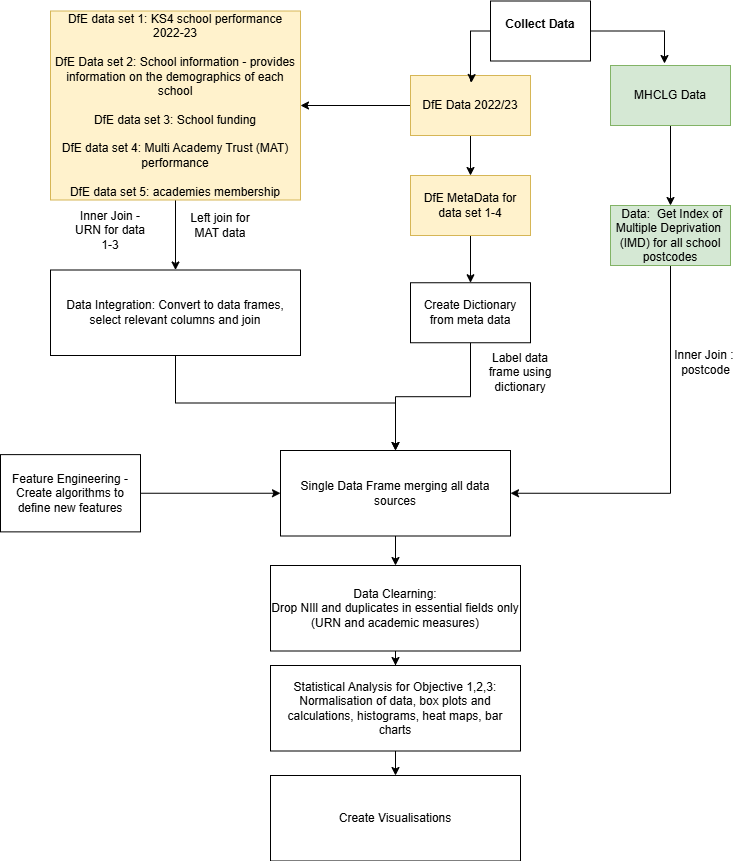
\includegraphics{P4DS_A2_Data_Analysis_Project_files/figure-pdf/cell-10-1-Pipeline.drawio.png}

}

\caption{Pipeline.drawio.png}

\end{figure}%

For a more dynamics view, workflow diagram can also be viewed
\href{https://padlet.com/saqib_safdar/saqib-safdar-pipleline-and-workflow-w1f0iib7imo5jrkg}{here}

\subsubsection{Processing Modules and
Algorithms}\label{processing-modules-and-algorithms}

The following modules and algrorithms will be required in a number of
instances and therefore defined and written within a class:

\begin{itemize}
\tightlist
\item
  \textbf{Class: DataWrangler} - load data from CSV, Excel file or
  existing pands data frame
\end{itemize}

Methods: - Load a csv file into a pandas dataframe using load\_csv
method - Load an excel file into a pandas dataframe using load\_excel
method - Create a dictionary from a dataframe using make\_dictionary
method - Rename columns in a dataframe using a dictionary using
column\_rename method - substitute original column names with
descriptive names in a dictionary or list - Convert percentage strings
in specified columns to float values using convert\_percentage\_columns
method - Retrieve specific columns from a given dataframe using a set of
URNs using get\_school\_details method

\begin{itemize}
\tightlist
\item
  Plot boxplots, histograms, heatmaps and scatter plots to visualise the
  data
\item
  Write code to generate summary statistics of the boxplots
\end{itemize}

\section{Program Code}\label{program-code}

\subsection{Libraries}\label{libraries}

I will begin by by importing the needed libraries for converting data to
dataframes, conducting calculations and visualisations

\begin{Shaded}
\begin{Highlighting}[]
\ImportTok{import}\NormalTok{ pandas }\ImportTok{as}\NormalTok{ pd}
\ImportTok{import}\NormalTok{ numpy }\ImportTok{as}\NormalTok{ np}
\ImportTok{import}\NormalTok{ statsmodels.api }\ImportTok{as}\NormalTok{ sm }
\ImportTok{import}\NormalTok{ matplotlib.pyplot }\ImportTok{as}\NormalTok{ plt}
\ImportTok{import}\NormalTok{ seaborn }\ImportTok{as}\NormalTok{ sns}
\ImportTok{from}\NormalTok{ scipy }\ImportTok{import}\NormalTok{ stats}
\ImportTok{import}\NormalTok{ os}
\ImportTok{from}\NormalTok{ sklearn.preprocessing }\ImportTok{import}\NormalTok{ StandardScaler }
\end{Highlighting}
\end{Shaded}

\subsection{Classes}\label{classes}

A class called Dataloader will be created to manage all core functions
related to data loading and wrangling. This includes:

\begin{itemize}
\tightlist
\item
  load\_csv
\item
  load\_excel
\item
  make\_dictionary
\item
  column\_rename
\item
  convert\_percentages\_column
\end{itemize}

Details of the functions purpose, paramters and return value can be read
in the doctrings below the function defintion

\begin{Shaded}
\begin{Highlighting}[]
\KeywordTok{class}\NormalTok{ DataWrangler: }
    \KeywordTok{def} \FunctionTok{\_\_init\_\_}\NormalTok{(}\VariableTok{self}\NormalTok{, file\_path}\OperatorTok{=}\VariableTok{None}\NormalTok{, dataframe}\OperatorTok{=}\VariableTok{None}\NormalTok{):}
        \CommentTok{"""}
\CommentTok{        Initialise the DataWrangler with a file path or an existing DataFrame.}

\CommentTok{        Parameters:}
\CommentTok{        {-} file\_path (str): The path to the data file (CSV or Excel).}
\CommentTok{        {-} dataframe (pd.DataFrame): An existing DataFrame to work with.}
\CommentTok{        """}
        \ControlFlowTok{if}\NormalTok{ dataframe }\KeywordTok{is} \KeywordTok{not} \VariableTok{None}\NormalTok{:}
            \VariableTok{self}\NormalTok{.df }\OperatorTok{=}\NormalTok{ dataframe.copy()}
            \BuiltInTok{print}\NormalTok{(}\StringTok{"DataWrangler initialised with the provided DataFrame."}\NormalTok{)}
        \ControlFlowTok{elif}\NormalTok{ file\_path }\KeywordTok{is} \KeywordTok{not} \VariableTok{None}\NormalTok{:}
            \VariableTok{self}\NormalTok{.file\_path }\OperatorTok{=}\NormalTok{ file\_path}
            \VariableTok{self}\NormalTok{.df }\OperatorTok{=} \VariableTok{None}

            \ControlFlowTok{if} \VariableTok{self}\NormalTok{.file\_path.endswith(}\StringTok{"csv"}\NormalTok{):}
                \VariableTok{self}\NormalTok{.load\_csv()}
            \ControlFlowTok{elif} \VariableTok{self}\NormalTok{.file\_path.endswith(}\StringTok{".xlsx"}\NormalTok{):}
                \VariableTok{self}\NormalTok{.load\_excel()}
            \ControlFlowTok{else}\NormalTok{:}
                \ControlFlowTok{raise} \PreprocessorTok{ValueError}\NormalTok{(}\StringTok{"Unsupported file format. Please provide a CSV or Excel file."}\NormalTok{)}
        \ControlFlowTok{else}\NormalTok{:}
            \ControlFlowTok{raise} \PreprocessorTok{ValueError}\NormalTok{(}\StringTok{"Either file\_path or dataframe must be provided."}\NormalTok{)}

   
    \KeywordTok{def}\NormalTok{ load\_csv(}\VariableTok{self}\NormalTok{):}
        \CommentTok{"""}
\CommentTok{        Load a CSV file into a pandas DataFrame.}
\CommentTok{        """}
        \ControlFlowTok{try}\NormalTok{:}
            \VariableTok{self}\NormalTok{.df }\OperatorTok{=}\NormalTok{ pd.read\_csv(}\VariableTok{self}\NormalTok{.file\_path, encoding}\OperatorTok{=}\StringTok{\textquotesingle{}latin1\textquotesingle{}}\NormalTok{)}
            \BuiltInTok{print}\NormalTok{(}\SpecialStringTok{f"CSV file loaded successfully from }\SpecialCharTok{\{}\VariableTok{self}\SpecialCharTok{.}\NormalTok{file\_path}\SpecialCharTok{\}}\SpecialStringTok{"}\NormalTok{)}
        \ControlFlowTok{except} \PreprocessorTok{FileNotFoundError} \ImportTok{as}\NormalTok{ e:}
            \BuiltInTok{print}\NormalTok{(}\SpecialStringTok{f"Error loading CSV file: }\SpecialCharTok{\{}\NormalTok{e}\SpecialCharTok{\}}\SpecialStringTok{"}\NormalTok{)}

    
    \KeywordTok{def}\NormalTok{ load\_excel(}\VariableTok{self}\NormalTok{):}
        \CommentTok{"""}
\CommentTok{        Load an Excel file into a pandas DataFrame.}
\CommentTok{        """}
        \ControlFlowTok{try}\NormalTok{:}
            \VariableTok{self}\NormalTok{.df }\OperatorTok{=}\NormalTok{ pd.read\_excel(}\VariableTok{self}\NormalTok{.file\_path)}
            \BuiltInTok{print}\NormalTok{(}\SpecialStringTok{f"Excel file loaded successfully from }\SpecialCharTok{\{}\VariableTok{self}\SpecialCharTok{.}\NormalTok{file\_path}\SpecialCharTok{\}}\SpecialStringTok{"}\NormalTok{)}
        \ControlFlowTok{except} \PreprocessorTok{FileNotFoundError} \ImportTok{as}\NormalTok{ e:}
            \BuiltInTok{print}\NormalTok{(}\SpecialStringTok{f"Error loading Excel file: }\SpecialCharTok{\{}\NormalTok{e}\SpecialCharTok{\}}\SpecialStringTok{"}\NormalTok{)}
            \VariableTok{self}\NormalTok{.df }\OperatorTok{=} \VariableTok{None}


    \KeywordTok{def}\NormalTok{ make\_dictionary(}\VariableTok{self}\NormalTok{, key\_column: }\BuiltInTok{str}\NormalTok{, value\_column: }\BuiltInTok{str}\NormalTok{):}
        \CommentTok{"""}
\CommentTok{        Create a dictionary from two columns of the DataFrame.}

\CommentTok{        Parameters:}
\CommentTok{        {-} key\_column (str): The column to use as the dictionary key.}
\CommentTok{        {-} value\_column (str): The column to use as the dictionary value.}

\CommentTok{        Returns:}
\CommentTok{        {-} dict: A dictionary mapping keys to values.}
\CommentTok{        """}
        \ControlFlowTok{try}\NormalTok{:}
            \ControlFlowTok{return} \BuiltInTok{dict}\NormalTok{(}\BuiltInTok{zip}\NormalTok{(}\VariableTok{self}\NormalTok{.df[key\_column], }\VariableTok{self}\NormalTok{.df[value\_column])) }
        \ControlFlowTok{except} \PreprocessorTok{KeyError} \ImportTok{as}\NormalTok{ e:}
            \BuiltInTok{print}\NormalTok{(}\SpecialStringTok{f"Error: Key column not found in DataFrame: }\SpecialCharTok{\{}\NormalTok{e}\SpecialCharTok{\}}\SpecialStringTok{"}\NormalTok{)}
            \ControlFlowTok{return} \VariableTok{None}

    \KeywordTok{def}\NormalTok{ column\_rename(}\VariableTok{self}\NormalTok{, column\_dict: }\BuiltInTok{dict}\NormalTok{):}
        \CommentTok{"""}
\CommentTok{        Rename columns in the DataFrame using a provided dictionary.}

\CommentTok{        Parameters:}
\CommentTok{        {-} column\_dict (dict): A dictionary mapping original column names to new names.}

\CommentTok{        Returns:}
\CommentTok{        {-} pd.DataFrame: The DataFrame with renamed columns.}
\CommentTok{        """}
        \VariableTok{self}\NormalTok{.df }\OperatorTok{=} \VariableTok{self}\NormalTok{.df.rename(columns}\OperatorTok{=}\NormalTok{column\_dict)}
        \BuiltInTok{print}\NormalTok{(}\StringTok{"Columns renamed successfully."}\NormalTok{)}
        \ControlFlowTok{return} \VariableTok{self}\NormalTok{.df}

    
    \KeywordTok{def}\NormalTok{ convert\_percentage\_columns(}\VariableTok{self}\NormalTok{, columns):}
        \CommentTok{"""}
\CommentTok{        Remove \% sign form colums .}

\CommentTok{        Parameters:}
\CommentTok{        {-} columns (list): List of column names to convert.}

\CommentTok{        Returns:}
\CommentTok{        {-} pd.DataFrame: The DataFrame with converted columns.}
\CommentTok{        """}
        \ControlFlowTok{for}\NormalTok{ col }\KeywordTok{in}\NormalTok{ columns:}
            \CommentTok{\# Remove \textquotesingle{}\%\textquotesingle{} and convert to float}
            \VariableTok{self}\NormalTok{.df[col] }\OperatorTok{=} \VariableTok{self}\NormalTok{.df[col].astype(}\BuiltInTok{str}\NormalTok{).}\BuiltInTok{str}\NormalTok{.replace(}\StringTok{\textquotesingle{}\%\textquotesingle{}}\NormalTok{, }\StringTok{\textquotesingle{}\textquotesingle{}}\NormalTok{)}
            \BuiltInTok{print}\NormalTok{(}\SpecialStringTok{f"Column \textquotesingle{}}\SpecialCharTok{\{}\NormalTok{col}\SpecialCharTok{\}}\SpecialStringTok{\textquotesingle{} converted"}\NormalTok{)}
        \ControlFlowTok{return} \VariableTok{self}\NormalTok{.df}

  
    \KeywordTok{def}\NormalTok{ get\_school\_details(}\VariableTok{self}\NormalTok{, urn\_set, columns):}
        \CommentTok{""" }
\CommentTok{        Retrieve essential school details for specified URNs and columns.}

\CommentTok{        Parameters:}
\CommentTok{        {-} urn\_set (set): A set of URNs (Unique Reference Numbers) for schools.}
\CommentTok{        {-} columns (list): List of columns to include in the output.}

\CommentTok{        Returns:}
\CommentTok{        {-} pd.DataFrame: A DataFrame containing the specified details.}
\CommentTok{        """}
        \ControlFlowTok{return} \VariableTok{self}\NormalTok{.df[}\VariableTok{self}\NormalTok{.df[}\StringTok{\textquotesingle{}URN\textquotesingle{}}\NormalTok{].isin(urn\_set)][columns]}
\end{Highlighting}
\end{Shaded}

\subsection{Load Data}\label{load-data}

I will now load and examine the five data files from the DfE as pandas
data frames and do a quick inspection using .head(),info(), describe().
To avoid repetition, I will do a more thorough analyse of data types and
missing values later, once all the data is combined.

\begin{Shaded}
\begin{Highlighting}[]
\CommentTok{\# Beginning with MAT data:}
\NormalTok{ks4\_mat\_performance }\OperatorTok{=}\NormalTok{ DataWrangler(}\StringTok{\textquotesingle{}data/2022{-}2023\_england\_ks4{-}mats{-}performance.csv\textquotesingle{}}\NormalTok{)}
\NormalTok{ks4\_mat\_performance.df.head()}
\end{Highlighting}
\end{Shaded}

\begin{verbatim}
CSV file loaded successfully from data/2022-2023_england_ks4-mats-performance.csv
\end{verbatim}

\begin{longtable}[]{@{}llllllllllllllllllllll@{}}
\toprule\noalign{}
& TIME\_PERIOD & TIME\_IDENTIFIER & TRUST\_GROUP\_TYPE & TRUST\_NAME &
TRUST\_UID & TRUST\_ID & TRUST\_COMPANIES\_HOUSE\_NUMBER & TRUST\_UKPRN
& TRUST\_LEADREGION & INSTITUTIONS\_MATPTINC & ... & INSTITUTIONS\_INMAT
& NUMINST\_INMAT & NUMINST\_CONVERTER\_INMAT & NUMINST\_SPONSOR\_INMAT &
NUMINST\_FREE\_INMAT & NUMINST\_STUDIO\_INMAT & NUMINST\_UTC\_INMAT &
TPUP\_INMAT & PFSM6CLA1A\_INMAT & PNOTFSM6CLA1A\_INMAT \\
\midrule\noalign{}
\endhead
\bottomrule\noalign{}
\endlastfoot
0 & 202223 & AcademicYear & Multi-academy trusts & ACTIVATE LEARNING
EDUCATION TRUST & 15710 & TR02786 & 8707909 & 10060613 & South East &
139268;141111;142024;145155;145945;146375 & ... &
139268;141111;142024;145155;145945;146375 & 6 & 0 & 2 & 0 & 0 & 4 & 647
& 21\% & 79\% \\
1 & 202223 & AcademicYear & Multi-academy trusts & ACER TRUST & 15720 &
TR01414 & 9591931 & 10060976 & South East & 142104;143984;144008 & ... &
142104;143984;144008 & 3 & 3 & 0 & 0 & 0 & 0 & 548 & 14\% & 86\% \\
2 & 202223 & AcademicYear & Multi-academy trusts & RED KITE LEARNING
TRUST & 15727 & TR00969 & 7523507 & 10054307 & Yorkshire and the Humber
& 136497;138304;141883;146247 & ... & 136497;138304;141883;146247 & 4 &
2 & 1 & 1 & 0 & 0 & 810 & 22\% & 78\% \\
3 & 202223 & AcademicYear & Multi-academy trusts & CONSILIUM ACADEMIES &
15728 & TR00082 & 9495671 & 10061209 & North East &
138314;143059;143845;144199;144200;144937;1449... & ... &
138314;143059;143845;144199;144200;144937;1449... & 8 & 5 & 3 & 0 & 0 &
0 & 1150 & 40\% & 60\% \\
4 & 202223 & AcademicYear & Multi-academy trusts & BATLEY MULTI ACADEMY
TRUST & 15729 & TR00147 & 7732537 & 10059240 & Yorkshire and the Humber
& 137424;137487;142406 & ... & 137424;137487;142406 & 3 & 1 & 1 & 1 & 0
& 0 & 520 & 32\% & 68\% \\
\end{longtable}

\begin{Shaded}
\begin{Highlighting}[]
\CommentTok{\# Keystage 4 school performance data:}
\NormalTok{ks4\_school\_performance }\OperatorTok{=}\NormalTok{ DataWrangler(}\StringTok{\textquotesingle{}data/2022{-}2023\_england\_ks4final.csv\textquotesingle{}}\NormalTok{)}
\NormalTok{ks4\_school\_performance.df.head()}
\end{Highlighting}
\end{Shaded}

\begin{verbatim}
CSV file loaded successfully from data/2022-2023_england_ks4final.csv
\end{verbatim}

\begin{verbatim}
C:\Users\saqib\AppData\Local\Temp\ipykernel_37860\3754428246.py:32: DtypeWarning: Columns (52,54,56,109,110,323,324,325,326,327,328,329,330,331,332,497,498,507,508) have mixed types. Specify dtype option on import or set low_memory=False.
  self.df = pd.read_csv(self.file_path, encoding='latin1')
\end{verbatim}

\begin{longtable}[]{@{}llllllllllllllllllllll@{}}
\toprule\noalign{}
& RECTYPE & LEA & ESTAB & URN & SCHNAME & SCHNAME\_AC & ADDRESS1 &
ADDRESS2 & ADDRESS3 & TOWN & ... & TAVENT\_GFSM6CLA1A\_PTQ\_EE &
TAVENT\_GNFSM6CLA1A\_PTQ\_EE & TAVENT\_GFSM6CLA1A\_21\_PTQ\_EE &
TAVENT\_GNFSM6CLA1A\_21\_PTQ\_EE & TAVENT\_GFSM6CLA1A\_22\_PTQ\_EE &
TAVENT\_GNFSM6CLA1A\_22\_PTQ\_EE & TTOTENT\_E\_TOTAL\_PTQ\_EE &
TTOTENT\_E\_COVID\_IMPACTED\_PTQ\_EE &
PTOTENT\_E\_COVID\_IMPACTED\_PTQ\_EE & P8\_BANDING \\
\midrule\noalign{}
\endhead
\bottomrule\noalign{}
\endlastfoot
0 & 1 & 201.0 & 6007.0 & 100003.0 & City of London School & NaN & 107
Queen Victoria Street & NaN & NaN & London & ... & NP & NP & NaN & NaN &
NP & NP & 569.0 & 3.0 & 1\% & NaN \\
1 & 1 & 201.0 & 6005.0 & 100001.0 & City of London School for Girls &
NaN & St Giles\textquotesingle{} Terrace & Barbican & NaN & London & ...
& NP & NP & NaN & NaN & NP & NP & 606.0 & 5.0 & 1\% & NaN \\
2 & 1 & 201.0 & 6000.0 & 100544.0 & David Game College & NaN & 31 Jewry
Street & London & NaN & NaN & ... & NP & NP & NaN & NaN & NP & NP & 53.0
& 1.0 & 2\% & NaN \\
3 & 4 & 201.0 & NaN & NaN & NaN & NaN & NaN & NaN & NaN & NaN & ... &
NaN & NaN & NaN & NaN & NaN & NaN & NaN & NaN & NaN & NaN \\
4 & 1 & 202.0 & 4285.0 & 100053.0 & Acland Burghley School & NaN &
Burghley Road & NaN & NaN & London & ... & 7.0 & 8.1 & NaN & NaN & 7 &
8.2 & 1397.0 & 0.0 & 0\% & Average \\
\end{longtable}

\begin{Shaded}
\begin{Highlighting}[]
\CommentTok{\#School demographics data:}
\NormalTok{school\_demographics }\OperatorTok{=}\NormalTok{ DataWrangler(}\StringTok{\textquotesingle{}data/2022{-}2023\_england\_school\_information.csv\textquotesingle{}}\NormalTok{)}
\NormalTok{school\_demographics.df.rename(columns}\OperatorTok{=}\NormalTok{\{}\StringTok{\textquotesingle{}URN\textquotesingle{}}\NormalTok{: }\StringTok{\textquotesingle{}URN\textquotesingle{}}\NormalTok{\}, inplace}\OperatorTok{=}\VariableTok{True}\NormalTok{) }\CommentTok{\#correction to URN column name}
\NormalTok{school\_demographics.df.head()}
\end{Highlighting}
\end{Shaded}

\begin{verbatim}
CSV file loaded successfully from data/2022-2023_england_school_information.csv
\end{verbatim}

\begin{longtable}[]{@{}llllllllllllllllllllll@{}}
\toprule\noalign{}
& URN & LANAME & LA & ESTAB & LAESTAB & SCHNAME & STREET & LOCALITY &
ADDRESS3 & TOWN & ... & ISPRIMARY & ISSECONDARY & ISPOST16 & AGELOW &
AGEHIGH & GENDER & RELCHAR & ADMPOL & OFSTEDRATING & OFSTEDLASTINSP \\
\midrule\noalign{}
\endhead
\bottomrule\noalign{}
\endlastfoot
0 & 100000 & City of London & 201 & 3614 & 2013614 & The Aldgate School
& St James\textquotesingle s Passage & Duke\textquotesingle s Place &
NaN & London & ... & 1 & 0 & 0 & 3.0 & 11.0 & Mixed & Church of England
& Not applicable & Outstanding & 13-06-2024 \\
1 & 100001 & City of London & 201 & 6005 & 2016005 & City of London
School for Girls & St Giles\textquotesingle{} Terrace & Barbican & NaN &
London & ... & 1 & 1 & 1 & 7.0 & 18.0 & Girls & NaN & Selective & NaN &
NaN \\
2 & 100002 & City of London & 201 & 6006 & 2016006 & St
Paul\textquotesingle s Cathedral School & 2 New Change & NaN & NaN &
London & ... & 1 & 1 & 0 & 4.0 & 13.0 & Mixed & Church of England & Not
applicable & NaN & NaN \\
3 & 100003 & City of London & 201 & 6007 & 2016007 & City of London
School & 107 Queen Victoria Street & NaN & NaN & London & ... & 1 & 1 &
1 & 10.0 & 18.0 & Boys & NaN & Not applicable & NaN & NaN \\
4 & 100008 & Camden & 202 & 2019 & 2022019 & Argyle Primary School &
Tonbridge Street & NaN & NaN & London & ... & 1 & 0 & 0 & 3.0 & 11.0 &
Mixed & Does not apply & Not applicable & Good & 05-10-2022 \\
\end{longtable}

\begin{Shaded}
\begin{Highlighting}[]
\CommentTok{\# School funding data:}
\NormalTok{school\_funding }\OperatorTok{=}\NormalTok{ DataWrangler(}\StringTok{\textquotesingle{}data/20230126\_school\_level\_data\_csv.csv\textquotesingle{}}\NormalTok{)}
\NormalTok{school\_funding.df.rename(columns}\OperatorTok{=}\NormalTok{\{}\StringTok{\textquotesingle{}time\_period\textquotesingle{}}\NormalTok{: }\StringTok{\textquotesingle{}time\_period\textquotesingle{}}\NormalTok{\}, inplace}\OperatorTok{=}\VariableTok{True}\NormalTok{) }\CommentTok{\#correction to time period column}
\NormalTok{school\_funding.df.head()}
\end{Highlighting}
\end{Shaded}

\begin{verbatim}
CSV file loaded successfully from data/20230126_school_level_data_csv.csv
\end{verbatim}

\begin{longtable}[]{@{}llllllllllllllllllllll@{}}
\toprule\noalign{}
& time\_period & time\_identifier & geographic\_level & country\_code &
country\_name & old\_la\_code & new\_la\_code & la\_name & school\_ukprn
& school\_urn & ... & allocation\_per\_pupil & pupil\_premium &
pupil\_premium\_pupils & universal\_infant\_free\_school\_meals\_grant &
pe\_\&\_sport\_premium & pe\_\&\_sport\_premium\_pupils &
coronavirus\_recovery\_premium\_funding & School\_led\_tutoring\_funding
& schools\_supplementary\_grant & total\_funding \\
\midrule\noalign{}
\endhead
\bottomrule\noalign{}
\endlastfoot
0 & 202223 & Financial year & School & E92000001 & England & 301 &
E09000002 & Barking and Dagenham & 10000222 & 101247 & ... & 6658.346870
& 291560 & 296 & x & x & x & 81972 & 49248 & 249881 & 8542828.0 \\
1 & 202223 & Financial year & School & E92000001 & England & 301 &
E09000002 & Barking and Dagenham & 10000527 & 101241 & ... & 6817.784488
& 492993 & 501 & x & x & x & 148598 & 84024 & 389143 & 13420859.0 \\
2 & 202223 & Financial year & School & E92000001 & England & 301 &
E09000002 & Barking and Dagenham & 10071309 & 101202 & ... & 5524.276364
& 209135 & 151 & 44741 & 20720 & 472 & 21895 & 24138 & 80619 &
3439599.0 \\
3 & 202223 & Financial year & School & E92000001 & England & 301 &
E09000002 & Barking and Dagenham & 10071301 & 101231 & ... & 5542.356295
& 153735 & 111 & 29116 & 19540 & 354 & 17927 & 18117 & 62142 &
2633909.0 \\
4 & 202223 & Financial year & School & E92000001 & England & 301 &
E09000002 & Barking and Dagenham & 10029207 & 136028 & ... & 7127.415584
& 511215 & 519 & x & x & x & 164595 & 91017 & 288410 & 9836214.0 \\
\end{longtable}

\begin{Shaded}
\begin{Highlighting}[]
\CommentTok{\#Academies data which connect URN code to postcode}
\NormalTok{academies\_membership }\OperatorTok{=}\NormalTok{ DataWrangler(}\StringTok{\textquotesingle{}data/academiesmatmembership20220901.csv\textquotesingle{}}\NormalTok{)}
\NormalTok{academies\_membership.df.head()}
\end{Highlighting}
\end{Shaded}

\begin{verbatim}
CSV file loaded successfully from data/academiesmatmembership20220901.csv
\end{verbatim}

\begin{longtable}[]{@{}llllllllllllllllllllll@{}}
\toprule\noalign{}
& URN & DfE Number & EstablishmentNumber & Establishment UKPRN & LA
(code) & LA (name) & Group UID & Group ID & TypeOfEstablishment (code) &
TypeOfEstablishment (name) & ... & Group Town & Group County & Group
Postcode & HeadTitle (name) & HeadFirstName & HeadLastName & Ofsted Last
Inspection Date & OfstedRating (name) & Predecessor Establishment &
Successor Establishment \\
\midrule\noalign{}
\endhead
\bottomrule\noalign{}
\endlastfoot
0 & 136683.0 & 840/4054 & 4054.0 & 10033436.0 & 840.0 & County Durham &
1128.0 & TR02582 & 34.0 & Academy converter & ... & Harrow & 99.0 & HA2
9DS & Not recorded & Felicity Jane & Smith & 2018-10-31 & NaN & YES &
YES \\
1 & 140594.0 & 936/2341 & 2341.0 & 10044809.0 & 936.0 & Surrey & 1128.0
& TR02582 & 34.0 & Academy converter & ... & Harrow & 99.0 & HA2 9DS &
Mrs & Clare & Spires & 2019-02-27 & NaN & YES & NO \\
2 & 136354.0 & 925/3510 & 3510.0 & 10032221.0 & 925.0 & Lincolnshire &
2044.0 & TR00261 & 34.0 & Academy converter & ... & Bourne & 99.0 & PE10
9EP & Mrs & Sarah & Moore & 2021-07-08 & NaN & YES & NO \\
3 & 137036.0 & 381/5404 & 5404.0 & 10034739.0 & 381.0 & Calderdale &
2044.0 & TR00261 & 28.0 & Academy sponsor led & ... & Bourne & 99.0 &
PE10 9EP & Mrs & Rosalinda & Wood-Ives & 2022-03-17 & NaN & YES & NO \\
4 & 140214.0 & 925/2016 & 2016.0 & 10043499.0 & 925.0 & Lincolnshire &
2044.0 & TR00261 & 28.0 & Academy sponsor led & ... & Bourne & 99.0 &
PE10 9EP & Mrs & Sarah & Moore & 2017-04-27 & NaN & NO & NO \\
\end{longtable}

\subsection{Load Metadata and Make
Dictionaries}\label{load-metadata-and-make-dictionaries}

I will now load the meta-data for each data file. To determine what each
column in the data files means, I will create a dictionary using the
make\_dictionary function defined as part of the DataWrangler class. The
meta data is labeled after each associated data file with the addition
of `meta' at the end.

\begin{Shaded}
\begin{Highlighting}[]

\NormalTok{ks4\_mat\_performance\_meta }\OperatorTok{=}\NormalTok{ DataWrangler(}\StringTok{\textquotesingle{}data/ks4{-}mats{-}performance\_meta.csv\textquotesingle{}}\NormalTok{)}
\NormalTok{ks4\_mat\_performance\_dict }\OperatorTok{=}\NormalTok{ DataWrangler.make\_dictionary(ks4\_mat\_performance\_meta, }\StringTok{\textquotesingle{}Metafile heading\textquotesingle{}}\NormalTok{,}\StringTok{\textquotesingle{}Metafile description\textquotesingle{}}\NormalTok{)}

\NormalTok{ks4\_mat\_performance\_dict}
\end{Highlighting}
\end{Shaded}

\begin{verbatim}
CSV file loaded successfully from data/ks4-mats-performance_meta.csv
\end{verbatim}

\begin{verbatim}
{'TIME_PERIOD': nan,
 'TIME_IDENTIFIER': nan,
 'TRUST_GROUP_TYPE': 'Trust type',
 'TRUST_NAME': 'Trust name',
 'TRUST_UID': 'Trust Unique identifier',
 'TRUST_ID': 'Trust Identifier',
 'TRUST_COMPANIES_HOUSE_NUMBER': 'Trust companies house number',
 'TRUST_UKPRN': 'Trust UK provider reference number',
 'TRUST_LEADREGION': 'Trust lead region',
 'INSTITUTIONS_MATPTINC': 'URNs, included in performance measures',
 'NUMINST_MATPTINC': 'Number of academies in the trust, included in performance measures',
 'NUMINST_CONVERTER_MATPTINC': 'Number of converter academies, included in performance measures',
 'NUMINST_SPONSOR_MATPTINC': 'Number of sponsor-led academies, included in performance measures',
 'NUMINST_FREE_MATPTINC': 'Number of free school - mainstream academies, included in performance measures',
 'NUMINST_STUDIO_MATPTINC': 'Number of free school - studio schools, included in performance measures',
 'NUMINST_UTC_MATPTINC': 'Number of free school - UTCs, included in performance measures',
 'NUMINST_FSM6CLA1A_MATPTINC': 'Number of academies with disadvantaged pupils, included in performance measures',
 'NUMINST_3_MATPTINC': 'Number of academies that have been in the trust for 3 years, included in performance measures',
 'NUMINST_4_MATPTINC': 'Number of academies that have been in the trust for 4 years, included in performance measures',
 'NUMINST_5PLUS_MATPTINC': 'Number of academies that have been in the trust for 5 years or more, included in performance measures',
 'TPUP_MATPTINC': 'Number of pupils at the end of ks4, included in performance measures',
 'KS2ASS_MATPTINC': 'KS4 cohort average KS2 Scaled Score (average of English reading and maths), included in performance measures',
 'PFSM6CLA1A_MATPTINC': '% of pupils at the end of ks4 who are disadvantaged, included in performance measures',
 'PNOTFSM6CLA1A_MATPTINC': '% of pupils at the end of ks4 who are not disadvantaged, included in performance measures',
 'PEALGRP2_MATPTINC': '% of pupils at the end of ks4 with English as additional language (EAL), included in performance measures',
 'PSEN_ALL4_MATPTINC': '% of pupils at the end of ks4 with special educational needs (SEN) including those with or without an Education, health and care (EHC) plan, included in performance measures',
 'ATT8SCR_WGTAVG': 'Average Attainment 8 score per pupil at the end of KS4, weighted average',
 'P8MEACOV': '% of pupils at the end of ks4 included in Progress 8 measure',
 'P8MEA_WGTAVG': 'Progress 8 measure after adjustment for extreme scores, weighted average',
 'P8CILOW': 'Progress 8 lower 95% confidence interval for adjusted average',
 'P8CIUPP': 'Progress 8 upper 95% confidence interval for adjusted average',
 'PTL2BASICS_95_WGTAVG': '% of pupils at the end of KS4 achieving strong 9-5 passes in both English and mathematics GCSEs , weighted average',
 'EBACCAPS_WGTAVG': 'Average EBacc APS score per pupil at the end of KS4, weighted average',
 'PTEBACC_95_WGTAVG': '% of pupils at the end of KS4 achieving the English Baccalaureate with 9-5 passes, weighted average',
 'PTEBACC_94_WGTAVG': '% of pupils at the end of KS4 achieving the English Baccalaureate with 9-4 passes, weighted average',
 'PTEBACC_E_PTQ_EE_WGTAVG': '% of pupils at the end of KS4 with entries in all English Baccalaureate subject areas, weighted average',
 'ATT8SCR_WGTAVG_FSM6CLA1A': 'Average Attainment 8 score per disadvantaged pupil at the end of KS4, weighted average',
 'P8MEACOV_FSM6CLA1A': '% of disadvantaged pupils at the end of ks4 included in Progress 8 measure',
 'P8MEA_WGTAVG_FSM6CLA1A': 'Progress 8 measure after adjustment for extreme scores for disadvantaged pupils, weighted average',
 'P8CILOW_FSM6CLA1A': 'Progress 8 lower 95% confidence interval for adjusted average for disadvantaged pupils',
 'P8CIUPP_FSM6CLA1A': 'Progress 8 upper 95% confidence interval for adjusted average for disadvantaged pupils',
 'PTL2BASICS_95_WGTAVG_FSM6CLA1A': '% of disadvantaged pupils at the end of KS4 achieving strong 9-5 passes in both English and mathematics GCSEs , weighted average',
 'EBACCAPS_WGTAVG_FSM6CLA1A': 'Average EBacc APS score per disadvantaged pupil at the end of KS4, weighted average',
 'PTEBACC_95_WGTAVG_FSM6CLA1A': '% of disadvantaged pupils at the end of KS4 achieving the English Baccalaureate with 9-5 passes, weighted average',
 'PTEBACC_94_WGTAVG_FSM6CLA1A': '% of disadvantaged pupils at the end of KS4 achieving the English Baccalaureate with 9-4 passes, weighted average',
 'PTEBACC_E_PTQ_EE_WGTAVG_FSM6CLA1A': '% of disadvantaged pupils at the end of KS4 with entries in all English Baccalaureate subject areas, weighted average',
 'ATT8SCR_WGTAVG_NFSM6CLA1A': 'Average Attainment 8 score per non-disadvantaged pupil at the end of KS4, weighted average',
 'P8MEACOV_NFSM6CLA1A': '% of non-disadvantaged pupils at the end of ks4 included in Progress 8 measure',
 'P8MEA_WGTAVG_NFSM6CLA1A': 'Progress 8 measure after adjustment for extreme scores for non-disadvantaged pupils, weighted average',
 'P8CILOW_NFSM6CLA1A': 'Progress 8 lower 95% confidence interval for adjusted average for non-disadvantaged pupils',
 'P8CIUPP_NFSM6CLA1A': 'Progress 8 upper 95% confidence interval for adjusted average for non-disadvantaged pupils',
 'PTL2BASICS_95_WGTAVG_NFSM6CLA1A': '% of non-disadvantaged pupils at the end of KS4 achieving strong 9-5 passes in both English and mathematics GCSEs , weighted average',
 'EBACCAPS_WGTAVG_NFSM6CLA1A': 'Average EBacc APS score per non-disadvantaged pupil at the end of KS4, weighted average',
 'PTEBACC_95_WGTAVG_NFSM6CLA1A': '% of non-disadvantaged pupils at the end of KS4 achieving the English Baccalaureate with 9-5 passes, weighted average',
 'PTEBACC_94_WGTAVG_NFSM6CLA1A': '% of non-disadvantaged pupils at the end of KS4 achieving the English Baccalaureate with 9-4 passes, weighted average',
 'PTEBACC_E_PTQ_EE_WGTAVG_NFSM6CLA1A': '% of non-disadvantaged pupils at the end of KS4 with entries in all English Baccalaureate subject areas, weighted average',
 'P8_BANDING': 'Progress 8 banding shown on performance tables website',
 'INSTITUTIONS_INMAT': 'URNs, including mainstream academies not in performance measures',
 'NUMINST_INMAT': 'Number of academies in the trust, including those not in performance measures',
 'NUMINST_CONVERTER_INMAT': 'Number of converter academies, including those not in performance measures',
 'NUMINST_SPONSOR_INMAT': 'Number of sponsor-led academies, including those not in performance measures',
 'NUMINST_FREE_INMAT': 'Number of free school - mainstream academies, including those not in performance measures',
 'NUMINST_STUDIO_INMAT': 'Number of free school - studio schools, including those not in performance measures',
 'NUMINST_UTC_INMAT': 'Number of free school - UTCs, including those not in performance measures',
 'TPUP_INMAT': 'Number of pupils at the end of KS4, including those not in performance measures',
 'PFSM6CLA1A_INMAT': '% of pupils at the end of KS4 who are disadvantaged, including those not in performance measures',
 'PNOTFSM6CLA1A_INMAT': '% of pupils at the end of KS4 who are not disadvantaged, including those not in performance measures'}
\end{verbatim}

\begin{Shaded}
\begin{Highlighting}[]
\NormalTok{school\_demographics\_meta }\OperatorTok{=}\NormalTok{ DataWrangler(}\StringTok{\textquotesingle{}data\textbackslash{}school\_information\_meta.csv\textquotesingle{}}\NormalTok{)}
\NormalTok{school\_demographics\_dict }\OperatorTok{=}\NormalTok{  DataWrangler.make\_dictionary(school\_demographics\_meta,}\StringTok{\textquotesingle{}Field Name\textquotesingle{}}\NormalTok{, }\StringTok{\textquotesingle{}Description\textquotesingle{}}\NormalTok{)}
\NormalTok{school\_demographics\_dict}
\end{Highlighting}
\end{Shaded}

\begin{verbatim}
CSV file loaded successfully from data\school_information_meta.csv
\end{verbatim}

\begin{verbatim}
<>:1: SyntaxWarning: invalid escape sequence '\s'
<>:1: SyntaxWarning: invalid escape sequence '\s'
C:\Users\saqib\AppData\Local\Temp\ipykernel_37860\3609157132.py:1: SyntaxWarning: invalid escape sequence '\s'
  school_demographics_meta = DataWrangler('data\school_information_meta.csv')
\end{verbatim}

\begin{verbatim}
{'URN': 'School unique reference number',
 'LANAME': 'Local authority name',
 'LA': 'Local authority number',
 'ESTAB': 'Establishment number',
 'LAESTAB': 'DfE number',
 'SCHNAME': 'School name',
 'STREET': 'School address (1)',
 'LOCALITY': 'School address (2)',
 'ADDRESS3': 'School address (3)',
 'TOWN': 'School town',
 'POSTCODE': 'School postcode',
 'SCHSTATUS': 'School open / closed status',
 'OPENDATE': 'Open date of school (if opened on or after 1st September 2022)',
 'CLOSEDATE': 'Date the school closed',
 'MINORGROUP': 'Type of school / college eg maintained school',
 'SCHOOLTYPE': 'School Type eg Voluntary Aided school',
 'ISPRIMARY': 'Does the school provide primary education? ( 0 = No, 1 = Yes)',
 'ISSECONDARY': 'Does the school provide secondary education? ( 0 = No, 1 = Yes)',
 'ISPOST16': 'Does the school provide post 16 education? (  0 = No, 1 = Yes)',
 'AGELOW': 'Lowest age of entry',
 'AGEHIGH': 'Highest age of entry',
 'GENDER': "Indicates whether it's a mixed or single sex school",
 'RELCHAR': 'Religious character',
 'ADMPOL': 'Admissions Policy',
 'OFSTEDRATING': 'Ofsted rating',
 'OFSTEDLASTINSP': 'Ofsted last inspection date'}
\end{verbatim}

\begin{Shaded}
\begin{Highlighting}[]
\NormalTok{ks4\_school\_performance\_meta }\OperatorTok{=}\NormalTok{ DataWrangler(}\StringTok{\textquotesingle{}data/ks4\_meta.xlsx\textquotesingle{}}\NormalTok{) }\CommentTok{\# this is originally in .xlsx format}
\NormalTok{school\_performance\_dict }\OperatorTok{=}\NormalTok{ DataWrangler.make\_dictionary(ks4\_school\_performance\_meta, }\StringTok{\textquotesingle{}Metafile heading\textquotesingle{}}\NormalTok{,}\StringTok{\textquotesingle{}Metafile description\textquotesingle{}}\NormalTok{)}
\CommentTok{\#school\_performance\_dict[\textquotesingle{}URN\textquotesingle{}] = \textquotesingle{}URN\textquotesingle{}  \# keep the URN column as it is as this will be used to merge the dataframes}
\NormalTok{school\_performance\_dict}
\end{Highlighting}
\end{Shaded}

\begin{verbatim}
Excel file loaded successfully from data/ks4_meta.xlsx
\end{verbatim}

\begin{verbatim}
{'RECTYPE': 'Record type (1=mainstream school; 2=special school; 4=local authority; 5=National (all schools); 7=National (maintained schools))',
 'LEA': 'Local authority code (see separate list of local authorities and their codes)',
 'ESTAB': 'Establishment number',
 'URN': 'School Unique Reference Number',
 'SCHNAME': 'School name',
 'SCHNAME_AC': 'School now known as (used if the school has converted to an academy on or after 12 Sept 2022)',
 'ADDRESS1': 'School address (1)',
 'ADDRESS2': 'School address (2)',
 'ADDRESS3': 'School address (3)',
 'TOWN': 'School town',
 'PCODE': 'School postcode',
 'TELNUM': 'School telephone number',
 'PCON_CODE': 'Parliamentary constituency code',
 'PCON_NAME': 'Parliamentary constituency name',
 'CONTFLAG': "Contingency flag - school results 'significantly affected'. This field is zero for all schools.",
 'ICLOSE': 'Closed school flag (0=open; 1=closed; 2=pending closure)',
 'NFTYPE': 'School type (see separate list of abbreviations used in the tables)',
 'RELDENOM': 'School religious character',
 'ADMPOL': 'School admissions policy (self-declared by schools on Edubase)',
 'ADMPOL_PT': 'School admissions policy - new definition from 2019',
 'EGENDER': 'School gender of entry',
 'FEEDER': 'Indicates whether school is a feeder school for sixth form centre/consortia (0=No; 1=Yes)',
 'TABKS2': 'Indicates whether school is published in the primary school (key stage 2) performance tables (0=No; 1=Yes)',
 'TAB1618': 'Indicates whether school is published in the school and college (16-18) performance tables (0=No; 1=Yes)',
 'AGERANGE': 'Age range',
 'TOTPUPS': 'Number of pupils on roll (all ages)',
 'NUMBOYS': 'Total boys on roll (including part-time pupils)',
 'NUMGIRLS': 'Total girls on roll (including part-time pupils)',
 'TPUP': 'Number of pupils at the end of key stage 4',
 'BPUP': 'Number of boys at the end of key stage 4',
 'PBPUP': '% of pupils at the end of key stage 4 who are boys',
 'GPUP': 'Number of girls at the end of key stage 4',
 'PGPUP': '% of pupils at the end key stage 4 who are girls',
 'KS2ASS': 'KS4 cohort average KS2 Scaled Score (average of English reading and maths)',
 'TPRIORLO': 'Number of pupils at the end of key stage 4 with low prior attainment at the end of key stage 2',
 'PTPRIORLO': '% of pupils at the end of key stage 4 with low prior attainment at the end of key stage 2',
 'TPRIORAV': 'Number of pupils at the end of key stage 4 with middle prior attainment at the end of key stage 2',
 'PTPRIORAV': '% of pupils at the end of key stage 4 with middle prior attainment at the end of key stage 2',
 'TPRIORHI': 'Number of pupils at the end of key stage 4 with high prior attainment at the end of key stage 2',
 'PTPRIORHI': '% of pupils at the end of key stage 4 with high prior attainment at the end of key stage 2',
 'TFSM6CLA1A': 'Number of disadvantaged pupils at the end of key stage 4',
 'PTFSM6CLA1A': '% of pupils at the end of key stage 4 who are disadvantaged',
 'TNOTFSM6CLA1A': 'Number of non-disadvantaged pupils at the end of key stage 4',
 'PTNOTFSM6CLA1A': '% of pupils at the end of key stage 4 who are not disadvantaged',
 'TEALGRP2': 'Number of pupils at the end of key stage 4 with English as additional language (EAL)',
 'PTEALGRP2': '% of pupils at the end of key stage 4 with English as additional language (EAL)',
 'TEALGRP1': 'Number of pupils at the end of key stage 4 with English as their first language',
 'PTEALGRP1': '% of pupils at the end of key stage 4 with English as their first language',
 'TEALGRP3': 'Number of pupils at the end of key stage 4 whose first language is unclassified',
 'PTEALGRP3': '% of pupils at the end of key stage 4 whose first language is unclassified',
 'TNMOB': 'Number of pupils at the end of key stage 4 who are non-mobile',
 'PTNMOB': '% of pupils at the end of key stage 4 who are non-mobile',
 'SENE4': 'Number of pupils at the end of key stage 4 with special educational needs (SEN) with an Education, health and care (EHC) plan',
 'PSENE4': '% of pupils at the end of key stage 4 with special educational needs (SEN) with an Education, health and care (EHC) plan',
 'SEN_ALL4': 'Number of pupils at the end of key stage 4 with special educational needs (SEN) including those with or without an Education, health and care (EHC) plan',
 'PSEN_ALL4': '% of pupils at the end of key stage 4 with special educational needs (SEN) including those with or without an Education, health and care (EHC) plan',
 'SENK4': 'Number of pupils at the end of key stage 4 with special educational needs (SEN) without an Education, health and care (EHC) plan',
 'PSENK4': '% of pupils at the end of key stage 4 with special educational needs (SEN) without an Education, health and care (EHC) plan',
 'TOTATT8': 'Total sum of Attainment 8 scores',
 'ATT8SCR': 'Average Attainment 8 score per pupil',
 'TOTATT8ENG': 'Total sum of Attainment 8 scores for English element',
 'ATT8SCRENG': 'Average Attainment 8 score per pupil for English element',
 'TOTATT8MAT': 'Total sum of Attainment 8 scores for mathematics element',
 'ATT8SCRMAT': 'Average Attainment 8 score per pupil for mathematics element',
 'TOTATT8EBAC': 'Total sum of Attainment 8 scores for EBacc element',
 'ATT8SCREBAC': 'Average Attainment 8 score per pupil for EBacc element',
 'TOTATT8OPEN': 'Total sum of Attainment 8 scores for open element',
 'ATT8SCROPEN': 'Average Attainment 8 score per pupil for open element',
 'TOTATT8OPENG': 'Total sum of Attainment 8 scores for open element - GCSE only',
 'ATT8SCROPENG': 'Average Attainment 8 score per pupil for open element - GCSE only',
 'TOTATT8OPENNG': 'Total sum of Attainment 8 scores for open element - non-GCSE only',
 'ATT8SCROPENNG': 'Average Attainment 8 score per pupil for open element - non-GCSE only',
 'AVGEBACFILL': 'Average number of EBacc slots filled in Attainment 8 per pupil',
 'AVGOPENFILL': 'Average number of Open slots filled in Attainment 8 per pupil',
 'P8PUP': 'Number of pupils included in Progress 8 measure',
 'TP8ADJ': 'Number of pupils who have had P8 score adjusted in average',
 'P8MEACOV': '% of pupils at the end of key stage 4 included in Progress 8 measure',
 'P8MEA': 'Progress 8 measure after adjustment for extreme scores',
 'P8CILOW': 'Progress 8 lower 95% confidence interval for adjusted average',
 'P8CIUPP': 'Progress 8 upper 95% confidence interval for adjusted average',
 'P8MEA_ORIG': 'Progress 8 measure based on unadjusted pupil scores',
 'P8CILOW_ORIG': 'Progress 8 lower 95% confidence interval for unadjusted average',
 'P8CIUPP_ORIG': 'Progress 8 upper 95% confidence interval for unadjusted average',
 'P8MEAENG': 'Progress 8 measure for English element',
 'P8MEAENG_CILOW': 'Lower 95% confidence interval for Progress 8 English element',
 'P8MEAENG_CIUPP': 'Upper 95% confidence interval for Progress 8 English element',
 'P8MEAMAT': 'Progress 8 measure for mathematics element',
 'P8MEAMAT_CILOW': 'Lower 95% confidence interval for Progress 8 maths element',
 'P8MEAMAT_CIUPP': 'Upper 95% confidence interval for Progress 8 maths element',
 'P8MEAEBAC': 'Progress 8 measure for EBacc element',
 'P8MEAEBAC_CILOW': 'Lower 95% confidence interval for Progress 8 EBacc element',
 'P8MEAEBAC_CIUPP': 'Upper 95% confidence interval for Progress 8 EBacc element',
 'P8MEAOPEN': 'Progress 8 measure for open element',
 'P8MEAOPEN_CILOW': 'Lower 95% confidence interval for Progress 8 open element',
 'P8MEAOPEN_CIUPP': 'Upper 95% confidence interval for Progress 8 open element',
 'PTL2BASICS_94': '% of pupils achieving standard 9-4 passes in both English and mathematics GCSEs ',
 'PTL2BASICS_95': '% of pupils achieving strong 9-5 passes in both English and mathematics GCSEs ',
 'TOTEBACCAPS': 'Total EBacc APS score per pupil',
 'EBACCAPS': 'Average EBacc APS score per pupil',
 'EBACCAPS_FSM6CLA1A': 'Average EBacc APS score per disadvantaged pupil',
 'EBACCAPS_NFSM6CLA1A': 'Average EBacc APS score per non-disadvantaged pupil',
 'EBACCAPS_LO': 'Average EBacc APS score per pupil with low prior attainment',
 'EBACCAPS_MID': 'Average EBacc APS score per pupil with middle prior attainment',
 'EBACCAPS_HI': 'Average EBacc APS score per pupil with high prior attainment',
 'EBACCAPS_EAL': 'Average EBacc APS score per pupil for whom English is an additional language',
 'EBACCAPS_GIRLS': 'Average EBacc APS score per girl',
 'EBACCAPS_BOYS': 'Average EBacc APS score per boy',
 'EBACCAPS_NMOB': 'Average EBacc APS score per non-mobile pupil',
 'EBACCAPS_21': 'Average EBacc APS score per pupil in 2021',
 'EBACCAPS_FSM6CLA1A_21': 'Average EBacc APS score per disadvantaged pupil in 2021',
 'EBACCAPS_NFSM6CLA1A_21': 'Average EBacc APS score per non-disadvantaged pupil in 2021',
 'EBACCAPS_22': 'Average EBacc APS score per pupil in 2022',
 'EBACCAPS_FSM6CLA1A_22': 'Average EBacc APS score per disadvantaged pupil in 2022',
 'EBACCAPS_NFSM6CLA1A_22': 'Average EBacc APS score per non-disadvantaged pupil in 2022',
 'TEBACC_E_PTQ_EE': 'Number of key stage 4 pupils with entries in all English Baccalaureate subject areas',
 'PTEBACC_E_PTQ_EE': '% of key stage 4 pupils with entries in all English Baccalaureate subject areas',
 'PTEBACC_94': '% of pupils achieving the English Baccalaureate with 9-4 passes',
 'PTEBACC_95': '% of pupils achieving the English Baccalaureate with 9-5 passes',
 'TEBACENG_E_PTQ_EE': 'Number of pupils entering the English Baccalaureate English subject area',
 'PTEBACENG_E_PTQ_EE': '% of pupils entering the English Baccalaureate English subject area',
 'TEBACMAT_E_PTQ_EE': 'Number of pupils entering the English Baccalaureate Maths subject area',
 'PTEBACMAT_E_PTQ_EE': '% of pupils entering the English Baccalaureate Maths subject area',
 'TEBAC2SCI_E_PTQ_EE': 'Number of pupils entering the English Baccalaureate Science subject area',
 'PTEBAC2SCI_E_PTQ_EE': '%  of pupils entering the English Baccalaureate Science subject area',
 'TEBACHUM_E_PTQ_EE': 'Number of pupils entering the English Baccalaureate Humanities subject area',
 'PTEBACHUM_E_PTQ_EE': '%  of pupils entering the English Baccalaureate Humanities subject area',
 'TEBACLAN_E_PTQ_EE': 'Number of pupils entering the English Baccalaureate Language subject area',
 'PTEBACLAN_E_PTQ_EE': '%  of pupils entering the English Baccalaureate Language subject area',
 'PTEBACENG_94': '% of pupils achieving the EBacc English subject area with a standard 9-4 pass',
 'PTEBACENG_95': '% of pupils achieving the EBacc English subject area with a strong 9-5 pass ',
 'PTEBACMAT_94': ' % of pupils achieving the EBacc Maths subject area with a standard 9-4 pass ',
 'PTEBACMAT_95': ' % of pupils achieving the EBacc Maths subject area with a strong 9-5 pass ',
 'PTEBAC2SCI_94': ' % of entered pupils achieving the EBacc Science subject area with a 9-4 pass',
 'PTEBAC2SCI_95': ' % of entered pupils achieving the EBacc Science subject area with a 9-5 pass',
 'PTEBACHUM_94': ' % of entered pupils achieving the EBacc Humanities subject area with a 9-4 pass',
 'PTEBACHUM_95': ' % of entered pupils achieving the EBacc Humanities subject area with a 9-5 pass',
 'PTEBACLAN_94': ' % of entered pupils achieving the EBacc Language subject area with a 9-4 pass',
 'PTEBACLAN_95': ' % of entered pupils achieving the EBacc Language subject area with a 9-5 pass',
 'SCIVAPUP_PTQ_EE': 'Number of pupils included in English Baccalaureate Science Value Added measure ',
 'SCIVACOV_PTQ_EE': 'Coverage of the English Baccalaureate Science Value Added indicators of those who entered for science',
 'HUMVAPUP_PTQ_EE': 'Number of pupils included in English Baccalaureate Humanities Value Added measure ',
 'HUMVACOV_PTQ_EE': 'Coverage of the English Baccalaureate Humanities Value Added indicators of those who entered for humanities',
 'LANVAPUP_PTQ_EE': 'Number of pupils included in English Baccalaureate Language Value Added measure ',
 'LANVACOV_PTQ_EE': 'Coverage of the English Baccalaureate Language Value Added indicators of those who entered for languages',
 'SCIVAMEA_PTQ_EE': 'English Baccalaureate Science Value Added measure',
 'SCIVALOW_PTQ_EE': 'English Baccalaureate Science Value Added lower 95% confidence limit',
 'SCIVAUPP_PTQ_EE': 'English Baccalaureate Science Value Added upper 95% confidence limit',
 'HUMVAMEA_PTQ_EE': 'EBacc Humanities VA measure',
 'HUMVALOW_PTQ_EE': 'English Baccalaureate Humanities Value Added lower 95% confidence limit',
 'HUMVAUPP_PTQ_EE': 'English Baccalaureate Humanities Value Added upper 95% confidence limit',
 'LANVAMEA_PTQ_EE': 'English Baccalaureate Languages Value Added measure',
 'LANVALOW_PTQ_EE': 'English Baccalaureate Languages Value Added lower 95% confidence limit',
 'LANVAUPP_PTQ_EE': 'English Baccalaureate Languages Value Added upper 95% confidence limit',
 'TEBACENG_94': 'Number of pupils achieving EBacc English subject area with a standard 9-4 pass ',
 'TEBACENG_95': 'Number of pupils achieving EBacc English subject area with a strong 9-5 pass ',
 'TEBACMAT_94': 'Number of pupils achieving EBacc Maths subject area with a standard 9-4 pass ',
 'TEBACMAT_95': 'Number of pupils achieving EBacc Maths subject area with a strong 9-5 pass ',
 'TEBAC2SCI_94': 'Number of pupils achieving EBacc Science subject area with a 9-4 pass',
 'TEBAC2SCI_95': 'Number of pupils achieving EBacc Science subject area with a 9-5 pass',
 'TEBACHUM_94': 'Number of pupils achieving EBacc Humanities subject area with a 9-4 pass',
 'TEBACHUM_95': 'Number of pupils achieving EBacc Humanities subject area with a 9-5 pass',
 'TEBACLAN_94': 'Number of pupils achieving EBacc Language subject area with a 9-4 pass',
 'TEBACLAN_95': 'Number of pupils achieving EBacc Language subject area with a 9-5 pass',
 'TEBACC91': 'Number of pupils achieving the English Baccalaureate at grades 9-1',
 'PTEBACC91': ' % of pupils achieving the English Baccalaureate at grades 9-1 ',
 'TEBACENG91': 'Number of pupils achieving EBacc English subject area at grade 9-1',
 'PTEBACENG91': '% of pupils achieving the EBacc English subject area at grade 9-1',
 'TEBACMAT91': 'Number of pupils achieving EBacc Maths subject area at grade 9-1',
 'PTEBACMAT91': ' % of pupils achieving the EBacc Maths subject area at grade 9-1',
 'TEBAC2SCI91': 'Number of pupils achieving EBacc Science subject area with grades 9-1',
 'PTEBAC2SCI91': ' % entered pupils achieving the EBacc Science subject area with grades 9-1',
 'TEBACHUM91': 'Number of pupils achieving EBacc Humanities subject area with grades 9-1',
 'PTEBACHUM91': ' % entered pupils achieving the EBacc Humanities subject area with grades 9-1',
 'TEBACLAN91': 'Number of pupils achieving EBacc Language subject area with grades 9-1',
 'PTEBACLAN91': ' % of entered pupils achieving the EBacc Language subject area with grades 9-1',
 'ATT8SCR_FSM6CLA1A': 'Average Attainment 8 score per disadvantaged pupil',
 'P8PUP_FSM6CLA1A': 'Number of disadvantaged pupils in Progress 8 measure',
 'TP8ADJ_FSM6CLA1A': 'Number of disadvantaged pupils in progress measure with adjusted scores',
 'P8MEA_FSM6CLA1A': 'Adjusted Progress 8 measure - disadvantaged pupils',
 'P8CILOW_FSM6CLA1A': 'Adjusted Progress 8 lower 95% confidence interval - disadvantaged pupils',
 'P8CIUPP_FSM6CLA1A': 'Adjusted Progress 8 upper 95% confidence interval - disadvantaged pupils',
 'P8MEA_FSM6CLA1A_ORIG': 'Unadjusted Progress 8 measure - disadvantaged pupils',
 'P8CILOW_FSM6CLA1A_ORIG': 'Unadjusted Progress 8 lower 95% confidence interval - disadvantaged pupils',
 'P8CIUPP_FSM6CLA1A_ORIG': 'Unadjusted Progress 8 upper 95% confidence interval - disadvantaged pupils',
 'ATT8SCR_NFSM6CLA1A': 'Average Attainment 8 score per non-disadvantaged pupil',
 'P8PUP_NFSM6CLA1A': 'Number of non-disadvantaged pupils in Progress 8 measure',
 'TP8ADJ_NFSM6CLA1A': 'Number of non-disadvantaged pupils in progress measure with adjusted scores',
 'P8MEA_NFSM6CLA1A': 'Adjusted Progress 8 measure - non-disadvantaged pupils',
 'P8CILOW_NFSM6CLA1A': 'Progress 8 lower 95% confidence interval - non-disadvantaged pupils',
 'P8CIUPP_NFSM6CLA1A': 'Progress 8 upper 95% confidence interval - non-disadvantaged pupils',
 'P8MEA_NFSM6CLA1A_ORIG': 'Unadjusted Progress 8 measure - non-disadvantaged pupils',
 'P8CILOW_NFSM6CLA1A_ORIG': 'Unadjusted Progress 8 lower 95% confidence interval - non-disadvantaged pupils',
 'P8CIUPP_NFSM6CLA1A_ORIG': 'Unadjusted Progress 8 upper 95% confidence interval - non-disadvantaged pupils',
 'ATT8SCRENG_FSM6CLA1A': 'Average Attainment 8 score per disadvantaged pupil for English element',
 'P8MEAENG_FSM6CLA1A': 'Progress 8 measure for English element - disadvantaged pupils',
 'P8MEAENG_CILOW_FSM6CLA1A': 'Lower 95% confidence interval for Progress 8 English element for disadvantaged pupils',
 'P8MEAENG_CIUPP_FSM6CLA1A': 'Upper 95% confidence interval for Progress 8 English element for disadvantaged pupils',
 'ATT8SCRMAT_FSM6CLA1A': 'Average Attainment 8 score per disadvantaged pupil for mathematics element',
 'P8MEAMAT_FSM6CLA1A': 'Progress 8 measure for maths element - disadvantaged pupils',
 'P8MEAMAT_CILOW_FSM6CLA1A': 'Lower 95% confidence interval for Progress 8 maths element for disadvantaged pupils',
 'P8MEAMAT_CIUPP_FSM6CLA1A': 'Upper 95% confidence interval for Progress 8 maths element for disadvantaged pupils',
 'ATT8SCREBAC_FSM6CLA1A': 'Average Attainment 8 score per disadvantaged pupil for EBacc element',
 'P8MEAEBAC_FSM6CLA1A': 'Progress 8 measure for EBacc element - disadvantaged pupils',
 'P8MEAEBAC_CILOW_FSM6CLA1A': 'Lower 95% confidence interval for Progress 8 EBacc element for disadvantaged pupils',
 'P8MEAEBAC_CIUPP_FSM6CLA1A': 'Upper 95% confidence interval for Progress 8 EBacc element for disadvantaged pupils',
 'ATT8SCROPEN_FSM6CLA1A': 'Average Attainment 8 score per disadvantaged pupil for open element',
 'P8MEAOPEN_FSM6CLA1A': 'Progress 8 measure for open element - disadvantaged pupils',
 'P8MEAOPEN_CILOW_FSM6CLA1A': 'Lower 95% confidence interval for Progress 8 open element for disadvantaged pupils',
 'P8MEAOPEN_CIUPP_FSM6CLA1A': 'Upper 95% confidence interval for Progress 8 open element for disadvantaged pupils',
 'ATT8SCRENG_NFSM6CLA1A': 'Average Attainment 8 score per non-disadvantaged pupil for English element',
 'P8MEAENG_NFSM6CLA1A': 'Progress 8 measure for English element - non-disadvantaged pupils',
 'P8MEAENG_CILOW_NFSM6CLA1A': 'Lower 95% confidence interval for Progress 8 English element for non-disadvantaged pupils',
 'P8MEAENG_CIUPP_NFSM6CLA1A': 'Upper 95% confidence interval for Progress 8 English element for non-disadvantaged pupils',
 'ATT8SCRMAT_NFSM6CLA1A': 'Average Attainment 8 score per non-disadvantaged pupil for mathematics element',
 'P8MEAMAT_NFSM6CLA1A': 'Progress 8 measure for maths element - non-disadvantaged pupils',
 'P8MEAMAT_CILOW_NFSM6CLA1A': 'Lower 95% confidence interval for Progress 8 maths element for non-disadvantaged pupils',
 'P8MEAMAT_CIUPP_NFSM6CLA1A': 'Upper 95% confidence interval for Progress 8 maths element for non-disadvantaged pupils',
 'ATT8SCREBAC_NFSM6CLA1A': 'Average Attainment 8 score per non-disadvantaged pupil for EBacc element',
 'P8MEAEBAC_NFSM6CLA1A': 'Progress 8 measure for EBacc element - non-disadvantaged pupils',
 'P8MEAEBAC_CILOW_NFSM6CLA1A': 'Lower 95% confidence interval for Progress 8 EBacc element for non-disadvantaged pupils',
 'P8MEAEBAC_CIUPP_NFSM6CLA1A': 'Upper 95% confidence interval for Progress 8 EBacc element for non-disadvantaged pupils',
 'ATT8SCROPEN_NFSM6CLA1A': 'Average Attainment 8 score per non-disadvantaged pupil for open element',
 'P8MEAOPEN_NFSM6CLA1A': 'Progress 8 measure for open element - non-disadvantaged pupils',
 'P8MEAOPEN_CILOW_NFSM6CLA1A': 'Lower 95% confidence interval for Progress 8 open element for non-disadvantaged pupils',
 'P8MEAOPEN_CIUPP_NFSM6CLA1A': 'Upper 95% confidence interval for Progress 8 open element for non-disadvantaged pupils',
 'ATT8SCROPENG_FSM6CLA1A': 'Average Attainment 8 score per disadvantaged pupil for open element - GCSE only',
 'ATT8SCROPENNG_FSM6CLA1A': 'Average Attainment 8 score per disadvantaged pupil for open element - non-GCSE only',
 'ATT8SCROPENG_NFSM6CLA1A': 'Average Attainment 8 score per non-disadvantaged pupil for open element - GCSE only',
 'ATT8SCROPENNG_NFSM6CLA1A': 'Average Attainment 8 score per non-disadvantaged pupil for open element - non-GCSE only',
 'DIFFN_ATT8': 'Difference between Attainment 8 for disadvantaged pupils in school/LA and non-disadvantaged pupils nationally',
 'DIFFN_P8MEA': 'Difference between Progress 8 measure for disadvantaged pupils in school/LA and non-disadvantaged pupils nationally',
 'ATT8SCR_LO': 'Average Attainment 8 score per pupil with low prior attainment',
 'P8PUP_LO': 'Number of pupils with low prior attainment included in Progress 8 measure',
 'TP8ADJ_LO': 'Number of pupils with low prior attainments in progress measure with adjusted scores',
 'P8MEA_LO': 'Adjusted Progress 8 measure - pupils with low prior attainments',
 'P8CILOW_LO': 'Adjusted Progress 8 lower 95% confidence interval - pupils with low prior attainments',
 'P8CIUPP_LO': 'Adjusted Progress 8 upper 95% confidence interval - pupils with low prior attainments',
 'P8MEA_LO_ORIG': 'Unadjusted Progress 8 measure - pupils with low prior attainments',
 'P8CILOW_LO_ORIG': 'Unadjusted Progress 8 lower 95% confidence interval - pupils with low prior attainments',
 'P8CIUPP_LO_ORIG': 'Unadjusted Progress 8 upper 95% confidence interval - pupils with low prior attainments',
 'ATT8SCR_MID': 'Average Attainment 8 score per pupil with middle prior attainment',
 'P8PUP_MID': 'Number of pupils with middle prior attainment included in Progress 8 measure',
 'TP8ADJ_MID': 'Number of pupils with middle prior attainments in progress measure with adjusted scores',
 'P8MEA_MID': 'Adjusted Progress 8 measure - pupils with middle prior attainment',
 'P8CILOW_MID': 'Progress 8 lower 95% confidence interval - pupils with middle prior attainment',
 'P8CIUPP_MID': 'Progress 8 upper 95% confidence interval - pupils with middle prior attainment',
 'P8MEA_MID_ORIG': 'Unadjusted Progress 8 measure - pupils with middle prior attainments',
 'P8CILOW_MID_ORIG': 'Unadjusted Progress 8 lower 95% confidence interval - pupils with middle prior attainments',
 'P8CIUPP_MID_ORIG': 'Unadjusted Progress 8 upper 95% confidence interval - pupils with middle prior attainments',
 'ATT8SCR_HI': 'Average Attainment 8 score per pupil with high prior attainment',
 'P8PUP_HI': 'Number of pupils with high prior attainment included in Progress 8 measure',
 'TP8ADJ_HI': 'Number of pupils with high prior attainments in progress measure with adjusted scores',
 'P8MEA_HI': 'Adjusted Progress 8 measure - pupils with high prior attainment',
 'P8CILOW_HI': 'Progress 8 lower 95% confidence interval - pupils with high prior attainment',
 'P8CIUPP_HI': 'Progress 8 upper 95% confidence interval - pupils with high prior attainment',
 'P8MEA_HI_ORIG': 'Unadjusted Progress 8 measure - pupils with high prior attainments',
 'P8CILOW_HI_ORIG': 'Unadjusted Progress 8 lower 95% confidence interval - pupils with high prior attainments',
 'P8CIUPP_HI_ORIG': 'Unadjusted Progress 8 upper 95% confidence interval - pupils with high prior attainments',
 'ATT8SCR_EAL': 'Average Attainment 8 score per pupil for whom English is an additional language',
 'ATT8SCRENG_EAL': 'Average Attainment 8 score per pupil for whom English is an additional language for English element',
 'ATT8SCRMAT_EAL': 'Average Attainment 8 score per pupil for whom English is an additional language for mathematics element',
 'ATT8SCREBAC_EAL': 'Average Attainment 8 score per pupil for whom English is an additional language for EBacc element',
 'ATT8SCROPEN_EAL': 'Average Attainment 8 score per pupil for whom English is an additional language for open element',
 'ATT8SCROPENG_EAL': 'Average Attainment 8 score per pupil for whom English is an additional language - GCSE only',
 'ATT8SCROPENNG_EAL': 'Average Attainment 8 score per pupil for whom English is an additional language - non-GCSE only',
 'P8PUP_EAL': 'Number of pupils for whom English is an additional language included in Progress 8 measure',
 'TP8ADJ_EAL': 'Number of pupils for whom English is an additional language in progress measure with adjusted scores',
 'P8MEA_EAL': 'Adjusted Progress 8 measure - pupils for whom English is an additional language',
 'P8CILOW_EAL': 'Adjusted Progress 8 lower 95% confidence interval - pupils for whom English is an additional language',
 'P8CIUPP_EAL': 'Adjusted Progress 8 upper 95% confidence interval - pupils for whom English is an additional language',
 'P8MEA_EAL_ORIG': 'Unadjusted Progress 8 measure - pupils for whom English is an additional language',
 'P8CILOW_EAL_ORIG': 'Unadjusted Progress 8 lower 95% confidence interval - pupils for whom English is an additional language',
 'P8CIUPP_EAL_ORIG': 'Unadjusted Progress 8 upper 95% confidence interval - pupils for whom English is an additional language',
 'ATT8SCR_GIRLS': 'Average Attainment 8 score per girl',
 'ATT8SCRENG_GIRLS': 'Average Attainment 8 score per girl for English element',
 'ATT8SCRMAT_GIRLS': 'Average Attainment 8 score per girl for mathematics element',
 'ATT8SCREBAC_GIRLS': 'Average Attainment 8 score per girl for EBacc element',
 'ATT8SCROPEN_GIRLS': 'Average Attainment 8 score per girl for open element',
 'ATT8SCROPENG_GIRLS': 'Average Attainment 8 score per girl - GCSE only',
 'ATT8SCROPENNG_GIRLS': 'Average Attainment 8 score per girl - non-GCSE only',
 'P8PUP_GIRLS': 'Number of girls included in Progress 8 measure',
 'TP8ADJ_GIRLS': 'Number of girls in progress measure with adjusted scores',
 'P8MEA_GIRLS': 'Adjusted Progress 8 measure - girls',
 'P8CILOW_GIRLS': 'Adjusted Progress 8 lower 95% confidence interval - girls',
 'P8CIUPP_GIRLS': 'Adjusted Progress 8 upper 95% confidence interval - girls',
 'P8MEA_GIRLS_ORIG': 'Unadjusted Progress 8 measure - girls',
 'P8CILOW_GIRLS_ORIG': 'Unadjusted Progress 8 lower 95% confidence interval - girls',
 'P8CIUPP_GIRLS_ORIG': 'Unadjusted Progress 8 upper 95% confidence interval - girls',
 'ATT8SCR_BOYS': 'Average Attainment 8 score per boy',
 'ATT8SCRENG_BOYS': 'Average Attainment 8 score per boy for English element',
 'ATT8SCRMAT_BOYS': 'Average Attainment 8 score per boy for mathematics element',
 'ATT8SCREBAC_BOYS': 'Average Attainment 8 score per boy for EBacc element',
 'ATT8SCROPEN_BOYS': 'Average Attainment 8 score per boy for open element',
 'ATT8SCROPENG_BOYS': 'Average Attainment 8 score per boy - GCSE only',
 'ATT8SCROPENNG_BOYS': 'Average Attainment 8 score per boy - non-GCSE only',
 'P8PUP_BOYS': 'Number of boys included in Progress 8 measure',
 'TP8ADJ_BOYS': 'Number of boys in progress measure with adjusted scores',
 'P8MEA_BOYS': 'Adjusted Progress 8 measure - boys',
 'P8CILOW_BOYS': 'Adjusted Progress 8 lower 95% confidence interval - boys',
 'P8CIUPP_BOYS': 'Adjusted Progress 8 upper 95% confidence interval - boys',
 'P8MEA_BOYS_ORIG': 'Unadjusted Progress 8 measure - boys',
 'P8CILOW_BOYS_ORIG': 'Unadjusted Progress 8 lower 95% confidence interval - boys',
 'P8CIUPP_BOYS_ORIG': 'Unadjusted Progress 8 upper 95% confidence interval - boys',
 'ATT8SCR_NMOB': 'Average Attainment 8 score per non-mobile pupil',
 'ATT8SCRENG_NMOB': 'Average Attainment 8 score per non-mobile pupil for English element',
 'ATT8SCRMAT_NMOB': 'Average Attainment 8 score per non-mobile pupil for mathematics element',
 'ATT8SCREBAC_NMOB': 'Average Attainment 8 score per non-mobile pupil for EBacc element',
 'ATT8SCROPEN_NMOB': 'Average Attainment 8 score per non-mobile pupil for open element',
 'ATT8SCROPENG_NMOB': 'Average Attainment 8 score per non-mobile pupil - GCSE only',
 'ATT8SCROPENNG_NMOB': 'Average Attainment 8 score per non-mobile pupil - non-GCSE only',
 'P8PUP_NMOB': 'Number of non-mobile pupils included in Progress 8 measure',
 'TP8ADJ_NMOB': 'Number of non-mobile pupils in progress measure with adjusted scores',
 'P8MEA_NMOB': 'Adjusted Progress 8 measure - non-mobile pupils',
 'P8CILOW_NMOB': 'Adjusted Progress 8 lower 95% confidence interval - non-mobile pupils',
 'P8CIUPP_NMOB': 'Adjusted Progress 8 upper 95% confidence interval - non-mobile pupils',
 'P8MEA_NMOB_ORIG': 'Unadjusted Progress 8 measure - non-mobile pupils',
 'P8CILOW_NMOB_ORIG': 'Unadjusted Progress 8 lower 95% confidence interval - non-mobile pupils',
 'P8CIUPP_NMOB_ORIG': 'Unadjusted Progress 8 upper 95% confidence interval - non-mobile pupils',
 'ATT8SCR_21': 'Average Attainment 8 score per pupil  - 2021',
 'P8PUP_21': 'Number of pupils in progress measure  - 2021',
 'P8MEA_21': 'Progress 8 measure  - 2021',
 'P8CILOW_21': 'Progress 8 lower 95% confidence interval  - 2021',
 'P8CIUPP_21': 'Progress 8 upper 95% confidence interval - 2021',
 'ATT8SCR_FSM6CLA1A_21': 'Average Attainment 8 score per disadvantaged pupil - 2021',
 'P8PUP_FSM6CLA1A_21': 'Number of disadvantaged pupils in progress measure - 2021',
 'P8MEA_FSM6CLA1A_21': 'Progress 8 measure - disadvantaged pupils - 2021',
 'P8CILOW_FSM6CLA1A_21': 'Progress 8 lower 95% confidence interval - disadvantaged pupils - 2021',
 'P8CIUPP_FSM6CLA1A_21': 'Progress 8 upper 95% confidence interval - disadvantaged pupils - 2021',
 'ATT8SCR_NFSM6CLA1A_21': 'Average Attainment 8 score per non-disadvantaged pupil - 2021',
 'P8PUP_NFSM6CLA1A_21': 'Number of non-disadvantaged pupils in progress measure - 2021',
 'P8MEA_NFSM6CLA1A_21': 'Progress 8 measure - non-disadvantaged pupils - 2021',
 'P8CILOW_NFSM6CLA1A_21': 'Progress 8 lower 95% confidence interval - non-disadvantaged pupils - 2021',
 'P8CIUPP_NFSM6CLA1A_21': 'Progress 8 upper 95% confidence interval - non-disadvantaged pupils - 2021',
 'ATT8SCR_22': 'Average Attainment 8 score per pupil - 2022',
 'P8PUP_22': 'Number of pupils in progress measure - 2022',
 'P8MEA_22': 'Progress 8 measure - 2022',
 'P8CILOW_22': 'Progress 8 lower 95% confidence interval - 2022',
 'P8CIUPP_22': 'Progress 8 upper 95% confidence interva - 2022',
 'ATT8SCR_FSM6CLA1A_22': 'Average Attainment 8 score per disadvantaged pupil - 2022',
 'P8PUP_FSM6CLA1A_22': 'Number of disadvantaged pupils in progress measure - 2022',
 'P8MEA_FSM6CLA1A_22': 'Progress 8 measure - disadvantaged pupils - 2022',
 'P8CILOW_FSM6CLA1A_22': 'Progress 8 lower 95% confidence interval - disadvantaged pupils - 2022',
 'P8CIUPP_FSM6CLA1A_22': 'Progress 8 upper 95% confidence interval - disadvantaged pupils - 2022',
 'ATT8SCR_NFSM6CLA1A_22': 'Average Attainment 8 score per non-disadvantaged pupil  - 2022',
 'P8PUP_NFSM6CLA1A_22': 'Number of non-disadvantaged pupils in progress measure - 2022',
 'P8MEA_NFSM6CLA1A_22': 'Progress 8 measure - non-disadvantaged pupils - 2022',
 'P8CILOW_NFSM6CLA1A_22': 'Progress 8 lower 95% confidence interval - non-disadvantaged pupils - 2022',
 'P8CIUPP_NFSM6CLA1A_22': 'Progress 8 upper 95% confidence interval - non-disadvantaged pupils - 2022',
 'TEBACC_ELO_PTQ_EE': 'Number of pupils in low prior attainment band with entries in all EBacc subject areas ',
 'PTEBACC_ELO_PTQ_EE': 'EBacc entered % by low prior attainment',
 'PTEBACCLO_94': 'EBacc achieved % by low prior attainment - with standard 9-4 passes in English and maths ',
 'PTEBACCLO_95': 'EBacc achieved % by low prior attainment - with 9-5 passes',
 'TEBACC_EAV_PTQ_EE': 'Number of pupils in middle prior attainment band with entries in all EBacc subject areas ',
 'PTEBACC_EAV_PTQ_EE': 'EBacc entered % by middle prior attainment',
 'PTEBACCAV_94': 'EBacc achieved % by middle prior attainment - with 9-4 passes',
 'PTEBACCAV_95': 'EBacc achieved % by middle prior attainment - with 9-5 passes',
 'TEBACC_EHI_PTQ_EE': 'Number of pupils in high prior attainment band with entries in all EBacc subject areas ',
 'PTEBACC_EHI_PTQ_EE': 'EBacc entered % by high prior attainment',
 'PTEBACCHI_94': 'EBacc achieved % by high prior attainment - with 9-4 passes',
 'PTEBACCHI_95': 'EBacc achieved % by high prior attainment - with 9-5 passes',
 'PTEBACC_EFSM6CLA1A_PTQ_EE': '% of disadvantaged pupils entering all English Baccalaureate subject areas',
 'PTEBACC_ENFSM6CLA1A_PTQ_EE': ' % of non-disadvantaged pupils entering all English Baccalaureate subject areas',
 'PTEBACC_94_FSM6CLA1A': ' % of disadvantaged pupils achieving the English Baccalaureate - with 9-4 passes',
 'PTEBACC_95_FSM6CLA1A': ' % of disadvantaged pupils achieving the English Baccalaureate - with 9-5 passes',
 'PTEBACC_94_NFSM6CLA1A': ' % of non-disadvantaged pupils achieving the English Baccalaureate - with 9-4 passes',
 'PTEBACC_95_NFSM6CLA1A': ' % of non-disadvantaged pupils achieving the English Baccalaureate - with 9-5 passes',
 'SCIVAMEA_LO_PTQ_EE': 'English Baccalaureate Science Value Added measure for pupils with low prior attainment',
 'SCIVAMEA_MID_PTQ_EE': 'English Baccalaureate Science Value Added measure for pupils with middle prior attainment',
 'SCIVAMEA_HI_PTQ_EE': 'English Baccalaureate Science Value Added measure for pupils with high prior attainment',
 'SCIVAMEA_FSM6CLA1A_PTQ_EE': 'English Baccalaureate Science Value Added measure for disadvantaged pupils',
 'SCIVAMEA_NFSM6CLA1A_PTQ_EE': 'English Baccalaureate Science Value Added measure for non-disadvantaged pupils',
 'HUMVAMEA_LO_PTQ_EE': 'English Baccalaureate Humanities Value Added measure for pupils with low prior attainment',
 'HUMVAMEA_MID_PTQ_EE': 'English Baccalaureate Humanities Value Added measure for pupils with middle prior attainment',
 'HUMVAMEA_HI_PTQ_EE': 'English Baccalaureate Humanities Value Added measure for pupils with high prior attainment',
 'HUMVAMEA_FSM6CLA1A_PTQ_EE': 'English Baccalaureate Humanities Value Added measure for disadvantaged pupils',
 'HUMVAMEA_NFSM6CLA1A_PTQ_EE': 'English Baccalaureate Humanities Value Added measure for non-disadvantaged pupils',
 'LANVAMEA_LO_PTQ_EE': 'English Baccalaureate Languages Value Added measure for pupils with low prior attainment',
 'LANVAMEA_MID_PTQ_EE': 'English Baccalaureate Languages Value Added measure for pupils with middle prior attainment',
 'LANVAMEA_HI_PTQ_EE': 'English Baccalaureate Languages Value Added measure for pupils with high prior attainment',
 'LANVAMEA_FSM6CLA1A_PTQ_EE': 'English Baccalaureate Languages Value Added measure for disadvantaged pupils',
 'LANVAMEA_NFSM6CLA1A_PTQ_EE': 'English Baccalaureate Languages Value Added measure for non-disadvantaged pupils',
 'SCIVAUPP_FSM6CLA1A_PTQ_EE': 'Upper 95% confidence limit for English Baccalaureate Science Value Added measure for disadvantaged pupils',
 'SCIVALOW_FSM6CLA1A_PTQ_EE': 'Lower 95% confidence limit for English Baccalaureate Science Value Added measure for disadvantaged pupils',
 'SCIVAUPP_NFSM6CLA1A_PTQ_EE': 'Upper 95% confidence limit for English Baccalaureate Science Value Added measure for non-disadvantaged pupils',
 'SCIVALOW_NFSM6CLA1A_PTQ_EE': 'Lower 95% confidence limit for English Baccalaureate Science Value Added measure for non-disadvantaged pupils',
 'SCIVAUPP_LO_PTQ_EE': 'Upper 95% confidence limit for English Baccalaureate Science Value Added measure for pupils with low prior attainment',
 'SCIVALOW_LO_PTQ_EE': 'Lower 95% confidence limit for English Baccalaureate Science Value Added measure for pupils with low prior attainment',
 'SCIVAUPP_MID_PTQ_EE': 'Upper 95% confidence limit for English Baccalaureate Science Value Added measure for pupils with middle prior attainment',
 'SCIVALOW_MID_PTQ_EE': 'Lower 95% confidence limit for English Baccalaureate Science Value Added measure for pupils with middle prior attainment',
 'SCIVAUPP_HI_PTQ_EE': 'Upper 95% confidence limit for English Baccalaureate Science Value Added measure for pupils with high prior attainment',
 'SCIVALOW_HI_PTQ_EE': 'Lower 95% confidence limit for English Baccalaureate Science Value Added measure for pupils with high prior attainment',
 'HUMVAUPP_FSM6CLA1A_PTQ_EE': 'Upper 95% confidence limit for English Baccalaureate Humanities Value Added measure for disadvantaged pupils',
 'HUMVALOW_FSM6CLA1A_PTQ_EE': 'Lower 95% confidence limit for English Baccalaureate Humanities Value Added measure for disadvantaged pupils',
 'HUMVAUPP_NFSM6CLA1A_PTQ_EE': 'Upper 95% confidence limit for English Baccalaureate Humanities Value Added measure for non-disadvantaged pupils',
 'HUMVALOW_NFSM6CLA1A_PTQ_EE': 'Lower 95% confidence limit for English Baccalaureate Humanities Value Added measure for non-disadvantaged pupils',
 'HUMVAUPP_LO_PTQ_EE': 'Upper 95% confidence limit for English Baccalaureate Humanities Value Added measure for pupils with low prior attainment',
 'HUMVALOW_LO_PTQ_EE': 'Lower 95% confidence limit for English Baccalaureate Humanities Value Added measure for pupils with low prior attainment',
 'HUMVAUPP_MID_PTQ_EE': 'Upper 95% confidence limit for English Baccalaureate Humanities Value Added measure for pupils with middle prior attainment',
 'HUMVALOW_MID_PTQ_EE': 'Lower 95% confidence limit for English Baccalaureate Humanities Value Added measure for pupils with middle prior attainment',
 'HUMVAUPP_HI_PTQ_EE': 'Upper 95% confidence limit for English Baccalaureate Humanities Value Added measure for pupils with high prior attainment',
 'HUMVALOW_HI_PTQ_EE': 'Lower 95% confidence limit for English Baccalaureate Humanities Value Added measure for pupils with high prior attainment',
 'LANVAUPP_FSM6CLA1A_PTQ_EE': 'Upper 95% confidence limit for English Baccalaureate Languages Value Added measure for disadvantaged pupils',
 'LANVALOW_FSM6CLA1A_PTQ_EE': 'Lower 95% confidence limit for English Baccalaureate Languages Value Added measure for disadvantaged pupils',
 'LANVAUPP_NFSM6CLA1A_PTQ_EE': 'Upper 95% confidence limit for English Baccalaureate Languages Value Added measure for non-disadvantaged pupils',
 'LANVALOW_NFSM6CLA1A_PTQ_EE': 'Lower 95% confidence limit for English Baccalaureate Languages Value Added measure for non-disadvantaged pupils',
 'LANVAUPP_LO_PTQ_EE': 'Upper 95% confidence limit for English Baccalaureate Languages Value Added measure for pupils with low prior attainment',
 'LANVALOW_LO_PTQ_EE': 'Lower 95% confidence limit for English Baccalaureate Languages Value Added measure for pupils with low prior attainment',
 'LANVAUPP_MID_PTQ_EE': 'Upper 95% confidence limit for English Baccalaureate Languages Value Added measure for pupils with middle prior attainment',
 'LANVALOW_MID_PTQ_EE': 'Lower 95% confidence limit for English Baccalaureate Languages Value Added measure for pupils with middle prior attainment',
 'LANVAUPP_HI_PTQ_EE': 'Upper 95% confidence limit for English Baccalaureate Languages Value Added measure for pupils with high prior attainment',
 'LANVALOW_HI_PTQ_EE': 'Lower 95% confidence limit for English Baccalaureate Languages Value Added measure for pupils with high prior attainment',
 'PTEBACC_E_21_PTQ_EE': '% of pupils entering all English Baccalaureate subject areas in 2021',
 'PTEBACC_94_21': '% of KS4 pupils achieving the Ebacc - with standard 9-4 passes in English and maths in 2021',
 'PTEBACC_95_21': '% of KS4 pupils achieving the Ebacc - with strong 9-5 passes in English and maths in 2021',
 'PTEBACC_E_22_PTQ_EE': '% of  pupils entering all English Baccalaureate subject areas in 2022',
 'PTEBACC_94_22': '% of KS4 pupils achieving the Ebacc - with standard 9-4 passes in English and maths in 2022',
 'PTEBACC_95_22': '% of KS4 pupils achieving the Ebacc - with strong 9-5 passes in English and maths in 2022',
 'PBEBACC_E_PTQ_EE': '% of boys with entries in all English Baccalaureate subject areas',
 'PBEBACC_94': '% of KS4 boys achieving the Ebacc - with 9-4 passes',
 'PBEBACC_95': '% of KS4 boys achieving the Ebacc - with 9-5 passes',
 'PGEBACC_E_PTQ_EE': '% of girls with entries in all English Baccalaureate subject areas',
 'PGEBACC_94': '% of KS4 girls achieving the Ebacc - with 9-4 passes',
 'PGEBACC_95': '% of KS4 girls achieving the Ebacc - with 9-5 passes',
 'PTEBACC_ENMOB_PTQ_EE': '% of non-mobile pupils with entries in all English Baccalaureate subject areas',
 'PTEBACCNMOB_94': '% of non-mobile pupils achieving the English Baccalaureate with 9-4 passes',
 'PTEBACCNMOB_95': '% of non-mobile pupils achieving the English Baccalaureate with 9-5 passes',
 'PTEBACC_EEAL_PTQ_EE': '% of pupils for whom English is an additional language with entries in all English Baccalaureate subject areas',
 'PTEBACCEAL_94': '% of pupils for whom English as an additional language achieving the English Baccalaureate with 9-4 passes',
 'PTEBACCEAL_95': '% of pupils for whom English as an additional language achieving the English Baccalaureate with 9-5 passes',
 'PTEBACC_EFSM6CLA1A_21': '% of disadvantaged pupils entering all English Baccalaureate subject areas in 2021',
 'PTEBACC_94_FSM6CLA1A_21': '% of disadvantaged pupils achieving the English Baccalaureate at grades 9-4 in 2021',
 'PTEBACC_95_FSM6CLA1A_21': '% of disadvantaged pupils achieving the English Baccalaureate at grades 9-5 in 2021',
 'PTEBACC_ENFSM6CLA1A_21': '% of non-disadvantaged pupils entering all English Baccalaureate subject areas in 2021',
 'PTEBACC_94_NFSM6CLA1A_21': '% of non-disadvantaged pupils achieving the English Baccalaureate at grade 9-4 in 2021',
 'PTEBACC_95_NFSM6CLA1A_21': '% of non-disadvantaged pupils achieving the English Baccalaureate at grade 9-5 in 2021',
 'PTEBACC_EFSM6CLA1A_22': '% of disadvantaged pupils entering all English Baccalaureate subject areas in 2022',
 'PTEBACC_94_FSM6CLA1A_22': '% of disadvantaged pupils achieving the English Baccalaureate including 9-4 passes in English and maths in 2022',
 'PTEBACC_95_FSM6CLA1A_22': '% of disadvantaged pupils achieving the English Baccalaureate including 9-5 passes in English and maths in 2022',
 'PTEBACC_ENFSM6CLA1A_22': '% of non-disadvantaged pupils entering all English Baccalaureate subject areas in 2022',
 'PTEBACC_94_NFSM6CLA1A_22': '% of non-disadvantaged pupils achieving the English Baccalaureate including 9-4 passes in English and maths in 2022',
 'PTEBACC_95_NFSM6CLA1A_22': '% of non-disadvantaged pupils achieving the English Baccalaureate including 9-5 passes in English and maths in 2022',
 'PT5EM_94': '% of pupils achieving Level 2 threshold including standard passes 9-4 in both English and Maths GCSEs',
 'PT5EM_94_21': '% of pupils achieving Level 2 threshold including standard passes 9-4 in both English and Maths GCSEs in 2021',
 'PT5EM_94_22': '% of pupils achieving Level 2 threshold including standard passes 9-4 in both English and Maths GCSEs in 2022',
 'PTANYQ_PTQ_EE': '% of pupils achieving any qualifications',
 'PTL2BASICS_94_21': '% of pupils achieving 9-4 passes in GCSE English and maths in 2021',
 'PTL2BASICS_95_21': '% of pupils achieving 9-5 passes in GCSE English and maths in 2021',
 'PTL2BASICS_94_22': '% of pupils achieving 9-4 passes in GCSE English and maths in 2022',
 'PTL2BASICS_95_22': '% of pupils achieving 9-5 passes in GCSE English and maths in 2022',
 'PTFSM6CLA1ABASICS_94': '% of disadvantaged pupils achieving standard 9-4 passes in GCSE English and maths',
 'PTNOTFSM6CLA1ABASICS_94': '% of non-disadvantaged pupils achieving standard 9-4 passes in GCSE English and maths',
 'TBASICSLO_94': 'Number of pupils in low prior attainment band who achieved standard 9-4 passes in English and maths',
 'PTBASICSLO_94': '% of pupils in low prior attainment band who achieved standard 9-4 passes in English and maths',
 'TBASICSAV_94': 'Number of pupils in middle prior attainment band who achieved standard 9-4 passes in English and maths',
 'PTBASICSAV_94': '% pupils in middle prior attainment band who achieved standard 9-4 passes in English and maths',
 'TBASICSHI_94': 'Number of pupils in high prior attainment band who achieved standard 9-4 passes in English and maths',
 'PTBASICSHI_94': '% pupils in high prior attainment band who achieved standard 9-4 passes in English and maths',
 'PBL2BASICS_94': '% of boys achieving standard 9-4 passes in both English and mathematics GCSEs ',
 'PGL2BASICS_94': '% of girls achieving standard 9-4 passes in both English and mathematics GCSEs ',
 'PTL2BASICSEAL_94': '% of pupils achieving standard 9-4 passes in both English and mathematics GCSEs and for whom English is an additional language',
 'PTL2BASICSNMOB_94': '% of non-mobile pupils achieving standard 9-4 passes in both English and mathematics GCSEs',
 'PTFSM6CLA1ABASICS_95': '% of disadvantaged pupils achieving strong 9-5 passes in GCSE English and maths',
 'PTNOTFSM6CLA1ABASICS_95': '% of non-disadvantaged pupils achieving strong 9-5 passes in GCSE English and maths',
 'TBASICSLO_95': 'Number of pupils in low prior attainment band who achieved strong 9-5 passes in English and maths',
 'PTBASICSLO_95': '% of pupils in low prior attainment band who achieved strong 9-5 passes in English and maths',
 'TBASICSAV_95': 'Number of pupils in middle prior attainment band who achieved strong 9-5 passes in English and maths',
 'PTBASICSAV_95': '% pupils in middle prior attainment band who achieved strong 9-5 passes in English and maths',
 'TBASICSHI_95': 'Number of pupils in high prior attainment band who achieved strong 9-5 passes in English and maths',
 'PTBASICSHI_95': '% pupils in high prior attainment band who achieved strong 9-5 passes in English and maths',
 'PBL2BASICS_95': '% of boys achieving strong 9-5 passes in both English and mathematics GCSEs ',
 'PGL2BASICS_95': '% of girls achieving strong 9-5 passes in both English and mathematics GCSEs ',
 'PTL2BASICSEAL_95': '% of pupils achieving strong 9-5 passes in both English and mathematics GCSEs and for whom English is an additional language',
 'PTL2BASICSNMOB_95': '% of non-mobile pupils achieving strong 9-5 passes in both English and mathematics GCSEs',
 'PTFSM6CLA1ABASICS_94_21': '% of disadvantaged pupils achieving 9-4 in GCSE English and maths in 2021',
 'PTFSM6CLA1ABASICS_95_21': '% of disadvantaged pupils achieving 9-4 passes in GCSE English and maths in 2021',
 'PTNOTFSM6CLA1ABASICS_94_21': '% of non-disadvantaged pupils achieving 9-4 passes in GCSE English and maths in 2021',
 'PTNOTFSM6CLA1ABASICS_95_21': '% of non-disadvantaged pupils achieving 9-5 passes in GCSE English and maths in 2021',
 'PTFSM6CLA1ABASICS_94_22': '% of disadvantaged pupils achieving 9-4 passes in GCSE English and maths in 2022',
 'PTFSM6CLA1ABASICS_95_22': '% of disadvantaged pupils achieving 9-5 passes in GCSE English and maths in 2022',
 'PTNOTFSM6CLA1ABASICS_94_22': '% of non-disadvantaged pupils achieving 9-4 passes in GCSE English and maths in 2022',
 'PTNOTFSM6CLA1ABASICS_95_22': '% of non-disadvantaged pupils achieving 9-5 passes in GCSE English and maths in 2022',
 'PTmultiLan_E': '% of pupils entering more than one language',
 'PTtripleSci_E': '% of pupils entering biology, chemistry and physics',
 'TFSM6CLA1A_21': 'Number of disadvantaged pupils at the end of key stage 4 in 2021',
 'PTFSM6CLA1A_21': '% of pupils at the end of key stage 4 who were disadvantaged in 2021',
 'TNOTFSM6CLA1A_21': 'Number of non-disadvantaged pupils at the end of key stage 4 in 2021',
 'PTNOTFSM6CLA1A_21': '% of pupils at the end of key stage 4 who were not disadvantaged in 2021',
 'TFSM6CLA1A_22': 'Number of disadvantaged pupils in 2022',
 'PTFSM6CLA1A_22': '% of pupils who were disadvantaged in 2022',
 'TNOTFSM6CLA1A_22': 'Number of non-disadvantaged pupils in 2022',
 'PTNOTFSM6CLA1A_22': '% of pupils who were not disadvantaged in 2022',
 'TAVENT_E_3NG_PTQ_EE': 'Average number of KS4 entries per pupil',
 'TAVENT_E_3NG_LO_PTQ_EE': 'Average number of KS4 entries per pupil with low prior attainment',
 'TAVENT_E_3NG_MID_PTQ_EE': 'Average number of KS4 entries per pupil with middle prior attainment',
 'TAVENT_E_3NG_HI_PTQ_EE': 'Average number of KS4 entries per pupil with high prior attainment',
 'TAVENT_E_3NG_FSM6CLA1A_PTQ_EE': 'Average number of KS4 entries per disadvantaged pupil',
 'TAVENT_E_3NG_NFSM6CLA1A_PTQ_EE': 'Average number of KS4 entries per non-disadvantaged pupil',
 'TAVENT_EFSM6CLA1A_21_PTQ_EE': 'Average number of KS4 entries per disadvantaged pupil in 2021',
 'TAVENT_ENFSM6CLA1A_21_PTQ_EE': 'Average number of KS4 entries per non-disadvantaged pupil in 2021',
 'TAVENT_EFSM6CLA1A_22_PTQ_EE': 'Average number of KS4 entries per disadvantaged pupil in 2022',
 'TAVENT_ENFSM6CLA1A_22_PTQ_EE': 'Average number of KS4 entries per non-disadvantaged pupil in 2022',
 'TAVENT_G_PTQ_EE': 'Average number of GCSE entries per pupil',
 'TAVENT_GLO_PTQ_EE': 'Average number of GCSE entries per pupil with low prior attainment',
 'TAVENT_GAV_PTQ_EE': 'Average number of GCSE entries per pupil with middle prior attainment',
 'TAVENT_GHI_PTQ_EE': 'Average number of GCSE entries per pupil with high prior attainment',
 'TAVENT_GFSM6CLA1A_PTQ_EE': 'Average number of GCSE entries per disadvantaged pupil',
 'TAVENT_GNFSM6CLA1A_PTQ_EE': 'Average number of GCSE entries per non-disadvantaged pupil',
 'TAVENT_GFSM6CLA1A_21_PTQ_EE': 'Average number of GCSE entries per disadvantaged pupil in 2021',
 'TAVENT_GNFSM6CLA1A_21_PTQ_EE': 'Average number of GCSE entries per non-disadvantaged pupil in 2021',
 'TAVENT_GFSM6CLA1A_22_PTQ_EE': 'Average number of GCSE entries per disadvantaged pupil in 2022',
 'TAVENT_GNFSM6CLA1A_22_PTQ_EE': 'Average number of GCSE entries per non-disadvantaged pupil in 2022',
 'TTOTENT_E_TOTAL_PTQ_EE': 'Total volume of entries without discounting',
 'TTOTENT_E_COVID_IMPACTED_PTQ_EE': 'Total volume of covid-impacted entries without discounting',
 'PTOTENT_E_COVID_IMPACTED_PTQ_EE': '% of covid-impacted entries out of total number of entries',
 'P8_BANDING': 'Progress 8 banding shown on school performance tables website'}
\end{verbatim}

\begin{Shaded}
\begin{Highlighting}[]
\NormalTok{school\_funding\_meta }\OperatorTok{=}\NormalTok{ DataWrangler(}\StringTok{\textquotesingle{}data/funding\_meta.csv\textquotesingle{}}\NormalTok{) }\CommentTok{\# this is originally in .xlsx format}
\NormalTok{school\_funding\_dict }\OperatorTok{=}\NormalTok{ DataWrangler.make\_dictionary(school\_funding\_meta, }\StringTok{\textquotesingle{}Variable name\textquotesingle{}}\NormalTok{,}\StringTok{\textquotesingle{}Variable description\textquotesingle{}}\NormalTok{)}
\NormalTok{school\_funding\_dict}
\end{Highlighting}
\end{Shaded}

\begin{verbatim}
CSV file loaded successfully from data/funding_meta.csv
\end{verbatim}

\begin{verbatim}
{'academy': 'Academy?',
 'allocation_per_pupil': 'Allocation per Pupil',
 'basic_entitlement_ks3': 'Basic Entitlement KS3',
 'basic_entitlement_ks4': 'Basic Entitlement KS4',
 'basic_entitlement_primary': 'Basic Entitlement Primary',
 'basic_entitlement_total_funding': 'Basic Entitlement Total Funding',
 'coronavirus_recovery_premium_funding': 'Coronavirus (COVID-19) recovery premium funding',
 'deprivation_total_funding': 'Deprivation Total Funding',
 'eal_total_funding': 'EAL Total Funding',
 'exceptional_factors_total_funding': 'Exceptional Factors Total Funding',
 'fsm_funding': 'FSM Funding',
 'fsm6_funding': 'FSM6 Funding',
 'idaci_band_a': 'IDACI Band A',
 'idaci_band_b': 'IDACI Band B',
 'idaci_band_c': 'IDACI Band C',
 'idaci_band_d': 'IDACI Band D',
 'idaci_band_e': 'IDACI Band E',
 'idaci_band_f': 'IDACI Band F',
 'idaci_funding': 'IDACI Funding',
 'lac_total_funding': 'LAC Total Funding',
 'london_fringe': 'London Fringe',
 'lump_sum_total_funding': 'Lump Sum Total Funding',
 'mfg_protection_or_capping_scaling': 'MFG protection (+ve) or capping/scaling (-ve)',
 'minimum_per_pupil_funding': 'Minimum per pupil funding',
 'mobility_total_funding': 'Mobility Total Funding',
 'national_non_domestic_rates_funding': 'National Non Domestic Rates Funding',
 'notional_sen': 'Notional SEN',
 'pe_&_sport_premium': 'PE & Sport Premium funding',
 'pe_&_sport_premium_pupils': 'PE & Sport Premium pupils',
 'pfi_total_funding': 'PFI Total Funding',
 'prior_attainment_total_funding': 'Prior Attainment Total Funding',
 'pupil_premium': 'Pupil Premium funding',
 'pupil_premium_pupils': 'Pupil Premium pupils',
 'School_led_tutoring_funding': 'School-led tutoring funding',
 'school_phase': 'Phase',
 'school_type': 'School type',
 'school_ukprn': 'UKPRN',
 'schools_supplementary_grant': 'Schools Supplementary Grant funding',
 'sparsity_total_funding': 'Sparsity Total Funding',
 'split_site_total_funding': 'Split Site Total Funding',
 'total_funding': 'Total funding',
 'total_number_of_pupils': 'Total Number of Pupils (rounded)',
 'total_schools_block_allocation_(post_mfg)': 'Total Schools Block Allocation (Post MFG)',
 'total_schools_block_allocation_(pre_mfg)': 'Total Schools Block Allocation (Pre MFG)',
 'trust': 'Trust',
 'universal_infant_free_school_meals_grant': 'Universal Infant Free School Meals Grant funding'}
\end{verbatim}

\subsection{Select Columns from Data}\label{select-columns-from-data}

Before re-labeling the columns using the defintions in the dictionaries,
it will be more efficient to select the columns needed in each data
file. I shall therefor re-define each dataframe according to the
selected columns needed.

MAT Performance Data:

\begin{Shaded}
\begin{Highlighting}[]
\CommentTok{\#only the following columns are needed}

\NormalTok{ks4\_mat\_performance\_df }\OperatorTok{=}\NormalTok{ ks4\_mat\_performance.df[[}\StringTok{\textquotesingle{}TRUST\_NAME\textquotesingle{}}\NormalTok{,}\StringTok{\textquotesingle{}TRUST\_UID\textquotesingle{}}\NormalTok{, }\StringTok{\textquotesingle{}TRUST\_ID\textquotesingle{}}\NormalTok{, }\StringTok{\textquotesingle{}NUMINST\_MATPTINC\textquotesingle{}}\NormalTok{,}\StringTok{\textquotesingle{}TPUP\_MATPTINC\textquotesingle{}}\NormalTok{,}\StringTok{\textquotesingle{}ATT8SCR\_WGTAVG\textquotesingle{}}\NormalTok{, }\StringTok{\textquotesingle{}P8MEA\_WGTAVG\textquotesingle{}}\NormalTok{, }\StringTok{\textquotesingle{}TIME\_PERIOD\textquotesingle{}}\NormalTok{]]}
\NormalTok{ks4\_mat\_performance\_df.head()}
\end{Highlighting}
\end{Shaded}

\begin{longtable}[]{@{}lllllllll@{}}
\toprule\noalign{}
& TRUST\_NAME & TRUST\_UID & TRUST\_ID & NUMINST\_MATPTINC &
TPUP\_MATPTINC & ATT8SCR\_WGTAVG & P8MEA\_WGTAVG & TIME\_PERIOD \\
\midrule\noalign{}
\endhead
\bottomrule\noalign{}
\endlastfoot
0 & ACTIVATE LEARNING EDUCATION TRUST & 15710 & TR02786 & 6 & 647 & 40.4
& -0.68 & 202223 \\
1 & ACER TRUST & 15720 & TR01414 & 3 & 548 & 49.4 & 0.08 & 202223 \\
2 & RED KITE LEARNING TRUST & 15727 & TR00969 & 4 & 810 & 46.9 & 0.00 &
202223 \\
3 & CONSILIUM ACADEMIES & 15728 & TR00082 & 8 & 1150 & 37.5 & -0.86 &
202223 \\
4 & BATLEY MULTI ACADEMY TRUST & 15729 & TR00147 & 3 & 520 & 45.7 & 0.16
& 202223 \\
\end{longtable}

Keystage 4 School Performance Data:

\begin{Shaded}
\begin{Highlighting}[]
\CommentTok{\#following columns are key measures for school performance}
\NormalTok{ks4\_school\_performance\_df }\OperatorTok{=}\NormalTok{ ks4\_school\_performance.df[[}\StringTok{\textquotesingle{}URN\textquotesingle{}}\NormalTok{,}
    \StringTok{\textquotesingle{}ATT8SCR\textquotesingle{}}\NormalTok{,}
    \StringTok{\textquotesingle{}P8MEA\textquotesingle{}}\NormalTok{,}
    \StringTok{\textquotesingle{}PTFSM6CLA1A\_22\textquotesingle{}}\NormalTok{,}
    \StringTok{\textquotesingle{}PTNOTFSM6CLA1A\_22\textquotesingle{}}\NormalTok{, }
    \StringTok{\textquotesingle{}PTFSM6CLA1ABASICS\_95\textquotesingle{}}\NormalTok{, }\CommentTok{\#462}
    \StringTok{\textquotesingle{}PTNOTFSM6CLA1ABASICS\_95\textquotesingle{}}\NormalTok{,}
    \StringTok{\textquotesingle{}ATT8SCR\_NFSM6CLA1A\_22\textquotesingle{}}\NormalTok{,}
    \StringTok{\textquotesingle{}P8MEA\_NFSM6CLA1A\_22\textquotesingle{}}\NormalTok{,}
\StringTok{\textquotesingle{}ATT8SCR\_FSM6CLA1A\_22\textquotesingle{}}\NormalTok{,}
    \StringTok{\textquotesingle{}P8MEA\_FSM6CLA1A\_22\textquotesingle{}}\NormalTok{,}
    \StringTok{\textquotesingle{}P8MEAMAT\_FSM6CLA1A\textquotesingle{}}\NormalTok{,}
    \StringTok{\textquotesingle{}P8MEAENG\_FSM6CLA1A\textquotesingle{}}\NormalTok{,}
    \StringTok{\textquotesingle{}P8MEAMAT\_NFSM6CLA1A\textquotesingle{}}\NormalTok{,}
    \StringTok{\textquotesingle{}P8MEAENG\_NFSM6CLA1A\textquotesingle{}}
\NormalTok{    ]]}


\NormalTok{ks4\_school\_performance\_df.head()}
\end{Highlighting}
\end{Shaded}

\begin{longtable}[]{@{}llllllllllllllll@{}}
\toprule\noalign{}
& URN & ATT8SCR & P8MEA & PTFSM6CLA1A\_22 & PTNOTFSM6CLA1A\_22 &
PTFSM6CLA1ABASICS\_95 & PTNOTFSM6CLA1ABASICS\_95 &
ATT8SCR\_NFSM6CLA1A\_22 & P8MEA\_NFSM6CLA1A\_22 & ATT8SCR\_FSM6CLA1A\_22
& P8MEA\_FSM6CLA1A\_22 & P8MEAMAT\_FSM6CLA1A & P8MEAENG\_FSM6CLA1A &
P8MEAMAT\_NFSM6CLA1A & P8MEAENG\_NFSM6CLA1A \\
\midrule\noalign{}
\endhead
\bottomrule\noalign{}
\endlastfoot
0 & 100003.0 & 36.8 & NP & NP & NP & NP & NP & NP & NP & NP & NP & NP &
NP & NP & NP \\
1 & 100001.0 & 29.4 & NP & NP & NP & NP & NP & NP & NP & NP & NP & NP &
NP & NP & NP \\
2 & 100544.0 & 6.8 & NP & NP & NP & NP & NP & NP & NP & NP & NP & NP &
NP & NP & NP \\
3 & NaN & NaN & NaN & NaN & NaN & NaN & NaN & NaN & NaN & NaN & NaN &
NaN & NaN & NaN & NaN \\
4 & 100053.0 & 50.3 & -0.16 & 42\% & 58\% & 28\% & 74\% & 59.7 & 0.26 &
38 & -0.99 & -0.82 & -0.79 & 0.39 & 0.35 \\
\end{longtable}

School Demographics:

\begin{Shaded}
\begin{Highlighting}[]
\NormalTok{school\_demographics\_df }\OperatorTok{=}\NormalTok{ school\_demographics.df[[}\StringTok{\textquotesingle{}URN\textquotesingle{}}\NormalTok{,}\StringTok{\textquotesingle{}LANAME\textquotesingle{}}\NormalTok{,}\StringTok{\textquotesingle{}LA\textquotesingle{}}\NormalTok{,}\StringTok{\textquotesingle{}SCHOOLTYPE\textquotesingle{}}\NormalTok{,}\StringTok{\textquotesingle{}MINORGROUP\textquotesingle{}}\NormalTok{,}\StringTok{\textquotesingle{}RELCHAR\textquotesingle{}}\NormalTok{,}\StringTok{\textquotesingle{}ADMPOL\textquotesingle{}}\NormalTok{,}\StringTok{\textquotesingle{}GENDER\textquotesingle{}}\NormalTok{,}\StringTok{\textquotesingle{}OFSTEDRATING\textquotesingle{}}\NormalTok{, }\StringTok{\textquotesingle{}POSTCODE\textquotesingle{}}\NormalTok{]]}
\NormalTok{school\_demographics\_df.head()}
\end{Highlighting}
\end{Shaded}

\begin{longtable}[]{@{}lllllllllll@{}}
\toprule\noalign{}
& URN & LANAME & LA & SCHOOLTYPE & MINORGROUP & RELCHAR & ADMPOL &
GENDER & OFSTEDRATING & POSTCODE \\
\midrule\noalign{}
\endhead
\bottomrule\noalign{}
\endlastfoot
0 & 100000 & City of London & 201 & Voluntary aided school & Maintained
school & Church of England & Not applicable & Mixed & Outstanding & EC3A
5DE \\
1 & 100001 & City of London & 201 & Other independent school &
Independent school & NaN & Selective & Girls & NaN & EC2Y 8BB \\
2 & 100002 & City of London & 201 & Other independent school &
Independent school & Church of England & Not applicable & Mixed & NaN &
EC4M 9AD \\
3 & 100003 & City of London & 201 & Other independent school &
Independent school & NaN & Not applicable & Boys & NaN & EC4V 3AL \\
4 & 100008 & Camden & 202 & Community school & Maintained school & Does
not apply & Not applicable & Mixed & Good & WC1H 9EG \\
\end{longtable}

School Funding:

\begin{Shaded}
\begin{Highlighting}[]
\NormalTok{school\_funding\_df }\OperatorTok{=}\NormalTok{ school\_funding.df[[}\StringTok{\textquotesingle{}school\_urn\textquotesingle{}}\NormalTok{,}\StringTok{\textquotesingle{}fsm\_funding\textquotesingle{}}\NormalTok{,}\StringTok{\textquotesingle{}pupil\_premium\textquotesingle{}}\NormalTok{,}\StringTok{\textquotesingle{}pupil\_premium\_pupils\textquotesingle{}}\NormalTok{,}\StringTok{\textquotesingle{}School\_led\_tutoring\_funding\textquotesingle{}}\NormalTok{,}\StringTok{\textquotesingle{}total\_funding\textquotesingle{}}\NormalTok{]]}

\NormalTok{school\_funding\_df.head()}

\end{Highlighting}
\end{Shaded}

\begin{longtable}[]{@{}lllllll@{}}
\toprule\noalign{}
& school\_urn & fsm\_funding & pupil\_premium & pupil\_premium\_pupils &
School\_led\_tutoring\_funding & total\_funding \\
\midrule\noalign{}
\endhead
\bottomrule\noalign{}
\endlastfoot
0 & 101247 & 118662 & 291560 & 296 & 49248 & 8542828.0 \\
1 & 101241 & 198479 & 492993 & 501 & 84024 & 13420859.0 \\
2 & 101202 & 75028 & 209135 & 151 & 24138 & 3439599.0 \\
3 & 101231 & 55872 & 153735 & 111 & 18117 & 2633909.0 \\
4 & 136028 & 211782 & 511215 & 519 & 91017 & 9836214.0 \\
\end{longtable}

\begin{Shaded}
\begin{Highlighting}[]
\CommentTok{\#change column name}
\NormalTok{school\_funding\_df.rename(columns}\OperatorTok{=}\NormalTok{\{}\StringTok{\textquotesingle{}school\_urn\textquotesingle{}}\NormalTok{:}\StringTok{\textquotesingle{}URN\textquotesingle{}}\NormalTok{\}, inplace}\OperatorTok{=}\VariableTok{True}\NormalTok{) }\CommentTok{\# change column name to match the school demographics dataframe  to allow ease of merging }
\NormalTok{school\_funding\_df.head()}
\end{Highlighting}
\end{Shaded}

\begin{verbatim}
C:\Users\saqib\AppData\Local\Temp\ipykernel_37860\65584972.py:2: SettingWithCopyWarning: 
A value is trying to be set on a copy of a slice from a DataFrame

See the caveats in the documentation: https://pandas.pydata.org/pandas-docs/stable/user_guide/indexing.html#returning-a-view-versus-a-copy
  school_funding_df.rename(columns={'school_urn':'URN'}, inplace=True) # change column name to match the school demographics dataframe  to allow ease of merging
\end{verbatim}

\begin{longtable}[]{@{}lllllll@{}}
\toprule\noalign{}
& URN & fsm\_funding & pupil\_premium & pupil\_premium\_pupils &
School\_led\_tutoring\_funding & total\_funding \\
\midrule\noalign{}
\endhead
\bottomrule\noalign{}
\endlastfoot
0 & 101247 & 118662 & 291560 & 296 & 49248 & 8542828.0 \\
1 & 101241 & 198479 & 492993 & 501 & 84024 & 13420859.0 \\
2 & 101202 & 75028 & 209135 & 151 & 24138 & 3439599.0 \\
3 & 101231 & 55872 & 153735 & 111 & 18117 & 2633909.0 \\
4 & 136028 & 211782 & 511215 & 519 & 91017 & 9836214.0 \\
\end{longtable}

Academies Membership

\begin{itemize}
\tightlist
\item
  Only URN, Trust ID, School Name and Trust Name are needed
\end{itemize}

\begin{Shaded}
\begin{Highlighting}[]
\NormalTok{academies\_membership\_df }\OperatorTok{=}\NormalTok{ academies\_membership.df[[}\StringTok{\textquotesingle{}URN\textquotesingle{}}\NormalTok{,}\StringTok{\textquotesingle{}Group UID\textquotesingle{}}\NormalTok{,}\StringTok{\textquotesingle{}Group ID\textquotesingle{}}\NormalTok{,}\StringTok{\textquotesingle{}EstablishmentName\textquotesingle{}}\NormalTok{,}\StringTok{\textquotesingle{}Group Name\textquotesingle{}}\NormalTok{]]}
\NormalTok{academies\_membership\_df.info()}
\end{Highlighting}
\end{Shaded}

\begin{verbatim}
<class 'pandas.core.frame.DataFrame'>
RangeIndex: 12637 entries, 0 to 12636
Data columns (total 5 columns):
 #   Column             Non-Null Count  Dtype  
---  ------             --------------  -----  
 0   URN                12618 non-null  float64
 1   Group UID          12463 non-null  float64
 2   Group ID           12463 non-null  object 
 3   EstablishmentName  12618 non-null  object 
 4   Group Name         12463 non-null  object 
dtypes: float64(2), object(3)
memory usage: 493.8+ KB
\end{verbatim}

\subsection{Merging DfE Data}\label{merging-dfe-data}

I can now begin merging the various DfE data based on school URN

\subsubsection{Merge: school demographics and school
funding}\label{merge-school-demographics-and-school-funding}

\begin{Shaded}
\begin{Highlighting}[]
\NormalTok{school\_funding\_df.columns}
\NormalTok{school\_funding\_df.rename(columns}\OperatorTok{=}\NormalTok{\{}\StringTok{\textquotesingle{}school\_urn\textquotesingle{}}\NormalTok{: }\StringTok{\textquotesingle{}URN\textquotesingle{}}\NormalTok{\}, inplace}\OperatorTok{=}\VariableTok{True}\NormalTok{) }\CommentTok{\# change name of URN column}
\NormalTok{school\_funding\_df.columns}
\end{Highlighting}
\end{Shaded}

\begin{verbatim}
C:\Users\saqib\AppData\Local\Temp\ipykernel_37860\2541994176.py:2: SettingWithCopyWarning: 
A value is trying to be set on a copy of a slice from a DataFrame

See the caveats in the documentation: https://pandas.pydata.org/pandas-docs/stable/user_guide/indexing.html#returning-a-view-versus-a-copy
  school_funding_df.rename(columns={'school_urn': 'URN'}, inplace=True) # change name of URN column
\end{verbatim}

\begin{verbatim}
Index(['URN', 'fsm_funding', 'pupil_premium', 'pupil_premium_pupils',
       'School_led_tutoring_funding', 'total_funding'],
      dtype='object')
\end{verbatim}

\begin{Shaded}
\begin{Highlighting}[]

\CommentTok{\# Merge School Information with Funding Data}
\NormalTok{merged\_df }\OperatorTok{=}\NormalTok{ pd.merge(school\_demographics\_df, school\_funding\_df, on}\OperatorTok{=}\StringTok{\textquotesingle{}URN\textquotesingle{}}\NormalTok{, how}\OperatorTok{=}\StringTok{\textquotesingle{}inner\textquotesingle{}}\NormalTok{) }
\CommentTok{\#chosen an inner join, as having incomplete left or right fields will not be of use}
\BuiltInTok{print}\NormalTok{(}\StringTok{"School Demographics and Funding data merged."}\NormalTok{)}

\NormalTok{merged\_df.shape}
\end{Highlighting}
\end{Shaded}

\begin{verbatim}
School Demographics and Funding data merged.
\end{verbatim}

\begin{verbatim}
(19973, 15)
\end{verbatim}

\begin{Shaded}
\begin{Highlighting}[]
\NormalTok{merged\_df.columns}
\end{Highlighting}
\end{Shaded}

\begin{verbatim}
Index(['URN', 'LANAME', 'LA', 'SCHOOLTYPE', 'MINORGROUP', 'RELCHAR', 'ADMPOL',
       'GENDER', 'OFSTEDRATING', 'POSTCODE', 'fsm_funding', 'pupil_premium',
       'pupil_premium_pupils', 'School_led_tutoring_funding', 'total_funding'],
      dtype='object')
\end{verbatim}

\subsubsection{Merge MAT info}\label{merge-mat-info}

\begin{Shaded}
\begin{Highlighting}[]
 \CommentTok{\# Merge with MAT Performance}
\NormalTok{merged\_df }\OperatorTok{=}\NormalTok{ pd.merge(merged\_df, academies\_membership\_df, on}\OperatorTok{=}\NormalTok{ [}\StringTok{\textquotesingle{}URN\textquotesingle{}}\NormalTok{], how}\OperatorTok{=}\StringTok{\textquotesingle{}left\textquotesingle{}}\NormalTok{) }
\CommentTok{\# some schools may not have an academy therefore a left join}
\BuiltInTok{print}\NormalTok{(}\StringTok{"Merged with MAT Performance data."}\NormalTok{)}
\end{Highlighting}
\end{Shaded}

\begin{verbatim}
Merged with MAT Performance data.
\end{verbatim}

\begin{Shaded}
\begin{Highlighting}[]
\NormalTok{merged\_df[}\StringTok{\textquotesingle{}URN\textquotesingle{}}\NormalTok{].nunique() }\CommentTok{\# count how many unique schools exist and therefore if some are duplicated}
\end{Highlighting}
\end{Shaded}

\begin{verbatim}
19973
\end{verbatim}

Some of the URNs may be duplicates and will need to be dropped later on
when I conduct data cleaning.

\subsubsection{merge school performance}\label{merge-school-performance}

\begin{Shaded}
\begin{Highlighting}[]
\NormalTok{merged\_df }\OperatorTok{=}\NormalTok{ pd.merge(merged\_df, ks4\_school\_performance\_df, on}\OperatorTok{=}\StringTok{\textquotesingle{}URN\textquotesingle{}}\NormalTok{, how}\OperatorTok{=}\StringTok{\textquotesingle{}inner\textquotesingle{}}\NormalTok{)}
\CommentTok{\# inner join essential as having only \textquotesingle{}right\textquotesingle{} or \textquotesingle{}left\textquotesingle{} data wouldnt be of much use}
\BuiltInTok{print}\NormalTok{(}\StringTok{"School KS4 performance data merged."}\NormalTok{)}
\NormalTok{merged\_df.head()}
\end{Highlighting}
\end{Shaded}

\begin{verbatim}
School KS4 performance data merged.
\end{verbatim}

\begin{longtable}[]{@{}llllllllllllllllllllll@{}}
\toprule\noalign{}
& URN & LANAME & LA & SCHOOLTYPE & MINORGROUP & RELCHAR & ADMPOL &
GENDER & OFSTEDRATING & POSTCODE & ... & PTFSM6CLA1ABASICS\_95 &
PTNOTFSM6CLA1ABASICS\_95 & ATT8SCR\_NFSM6CLA1A\_22 &
P8MEA\_NFSM6CLA1A\_22 & ATT8SCR\_FSM6CLA1A\_22 & P8MEA\_FSM6CLA1A\_22 &
P8MEAMAT\_FSM6CLA1A & P8MEAENG\_FSM6CLA1A & P8MEAMAT\_NFSM6CLA1A &
P8MEAENG\_NFSM6CLA1A \\
\midrule\noalign{}
\endhead
\bottomrule\noalign{}
\endlastfoot
0 & 100049 & Camden & 202 & Community school & Maintained school & Does
not apply & Non-selective & Mixed & Good & NW3 2BQ & ... & 40\% & 48\% &
54.9 & 0.15 & 47 & -0.12 & -0.16 & -0.57 & 0.30 & 0.01 \\
1 & 100050 & Camden & 202 & Community school & Maintained school & Does
not apply & Non-selective & Girls & Outstanding & NW5 1RL & ... & 53\% &
76\% & 71.9 & 1.28 & 52.3 & 0.36 & -0.09 & 0.12 & 0.74 & 0.93 \\
2 & 100051 & Camden & 202 & Community school & Maintained school & Does
not apply & Non-selective & Mixed & Good & NW1 1RX & ... & 35\% & 48\% &
54.5 & 0.66 & 49.4 & 0.29 & -0.01 & -0.20 & 0.77 & 0.10 \\
3 & 100052 & Camden & 202 & Community school & Maintained school & Does
not apply & Non-selective & Mixed & Good & NW2 3RT & ... & 31\% & 53\% &
50.2 & 0.22 & 43.2 & 0.05 & -0.05 & -0.01 & 0.38 & 0.19 \\
4 & 100053 & Camden & 202 & Community school & Maintained school & Does
not apply & Non-selective & Mixed & Good & NW5 1UJ & ... & 28\% & 74\% &
59.7 & 0.26 & 38 & -0.99 & -0.82 & -0.79 & 0.39 & 0.35 \\
\end{longtable}

\begin{Shaded}
\begin{Highlighting}[]
\NormalTok{merged\_df[}\StringTok{\textquotesingle{}URN\textquotesingle{}}\NormalTok{].nunique()}
\end{Highlighting}
\end{Shaded}

\begin{verbatim}
3281
\end{verbatim}

Observation: The number of unique schools has dropped from 19k to 3k,
when the keystage 4 data was merged on an inner join. This is expected
as reportedly 3444 state-funded secondary schools in England, with
private schools included it is approximately 4175 {[}7{]}. Of these a
number by newly opened and not have delivered GCSE in 2022/23

{[}7{]} Tes. (2024, January 17). How many schools are there in the UK?
Retrieved from
https://www.tes.com/magazine/analysis/general/how-many-schools-in-the-uk

\subsubsection{merged MAT performance
data}\label{merged-mat-performance-data}

\begin{Shaded}
\begin{Highlighting}[]
\NormalTok{merged\_df }\OperatorTok{=}\NormalTok{ pd.merge(merged\_df, ks4\_mat\_performance\_df, left\_on}\OperatorTok{=}\NormalTok{[}\StringTok{\textquotesingle{}Group ID\textquotesingle{}}\NormalTok{], right\_on}\OperatorTok{=}\NormalTok{[}\StringTok{\textquotesingle{}TRUST\_ID\textquotesingle{}}\NormalTok{], how}\OperatorTok{=}\StringTok{\textquotesingle{}left\textquotesingle{}}\NormalTok{)}
\BuiltInTok{print}\NormalTok{(}\StringTok{"Merged with MAT Performance data."}\NormalTok{)}
\end{Highlighting}
\end{Shaded}

\begin{verbatim}
Merged with MAT Performance data.
\end{verbatim}

\begin{Shaded}
\begin{Highlighting}[]
\NormalTok{merged\_df.info()}
\end{Highlighting}
\end{Shaded}

\begin{verbatim}
<class 'pandas.core.frame.DataFrame'>
RangeIndex: 3866 entries, 0 to 3865
Data columns (total 41 columns):
 #   Column                       Non-Null Count  Dtype  
---  ------                       --------------  -----  
 0   URN                          3866 non-null   int64  
 1   LANAME                       3866 non-null   object 
 2   LA                           3866 non-null   int64  
 3   SCHOOLTYPE                   3866 non-null   object 
 4   MINORGROUP                   3866 non-null   object 
 5   RELCHAR                      2399 non-null   object 
 6   ADMPOL                       3601 non-null   object 
 7   GENDER                       3866 non-null   object 
 8   OFSTEDRATING                 3822 non-null   object 
 9   POSTCODE                     3866 non-null   object 
 10  fsm_funding                  3866 non-null   int64  
 11  pupil_premium                3866 non-null   object 
 12  pupil_premium_pupils         3866 non-null   object 
 13  School_led_tutoring_funding  3866 non-null   object 
 14  total_funding                3866 non-null   float64
 15  Group UID                    3214 non-null   float64
 16  Group ID                     3214 non-null   object 
 17  EstablishmentName            3214 non-null   object 
 18  Group Name                   3214 non-null   object 
 19  ATT8SCR                      3807 non-null   object 
 20  P8MEA                        3807 non-null   object 
 21  PTFSM6CLA1A_22               3770 non-null   object 
 22  PTNOTFSM6CLA1A_22            3770 non-null   object 
 23  PTFSM6CLA1ABASICS_95         3807 non-null   object 
 24  PTNOTFSM6CLA1ABASICS_95      3807 non-null   object 
 25  ATT8SCR_NFSM6CLA1A_22        3770 non-null   object 
 26  P8MEA_NFSM6CLA1A_22          3770 non-null   object 
 27  ATT8SCR_FSM6CLA1A_22         3770 non-null   object 
 28  P8MEA_FSM6CLA1A_22           3770 non-null   object 
 29  P8MEAMAT_FSM6CLA1A           3807 non-null   object 
 30  P8MEAENG_FSM6CLA1A           3807 non-null   object 
 31  P8MEAMAT_NFSM6CLA1A          3807 non-null   object 
 32  P8MEAENG_NFSM6CLA1A          3807 non-null   object 
 33  TRUST_NAME                   1346 non-null   object 
 34  TRUST_UID                    1346 non-null   float64
 35  TRUST_ID                     1346 non-null   object 
 36  NUMINST_MATPTINC             1346 non-null   float64
 37  TPUP_MATPTINC                1346 non-null   float64
 38  ATT8SCR_WGTAVG               1346 non-null   float64
 39  P8MEA_WGTAVG                 1346 non-null   float64
 40  TIME_PERIOD                  1346 non-null   float64
dtypes: float64(8), int64(3), object(30)
memory usage: 1.2+ MB
\end{verbatim}

\subsection{Data Cleaning}\label{data-cleaning}

Now that the merging is complete, I can now remove rows which are note
needed

\subsubsection{Remove NaN values}\label{remove-nan-values}

\begin{Shaded}
\begin{Highlighting}[]
\NormalTok{merged\_df.isna().}\BuiltInTok{sum}\NormalTok{()}
\end{Highlighting}
\end{Shaded}

\begin{verbatim}
URN                               0
LANAME                            0
LA                                0
SCHOOLTYPE                        0
MINORGROUP                        0
RELCHAR                        1467
ADMPOL                          265
GENDER                            0
OFSTEDRATING                     44
POSTCODE                          0
fsm_funding                       0
pupil_premium                     0
pupil_premium_pupils              0
School_led_tutoring_funding       0
total_funding                     0
Group UID                       652
Group ID                        652
EstablishmentName               652
Group Name                      652
ATT8SCR                          59
P8MEA                            59
PTFSM6CLA1A_22                   96
PTNOTFSM6CLA1A_22                96
PTFSM6CLA1ABASICS_95             59
PTNOTFSM6CLA1ABASICS_95          59
ATT8SCR_NFSM6CLA1A_22            96
P8MEA_NFSM6CLA1A_22              96
ATT8SCR_FSM6CLA1A_22             96
P8MEA_FSM6CLA1A_22               96
P8MEAMAT_FSM6CLA1A               59
P8MEAENG_FSM6CLA1A               59
P8MEAMAT_NFSM6CLA1A              59
P8MEAENG_NFSM6CLA1A              59
TRUST_NAME                     2520
TRUST_UID                      2520
TRUST_ID                       2520
NUMINST_MATPTINC               2520
TPUP_MATPTINC                  2520
ATT8SCR_WGTAVG                 2520
P8MEA_WGTAVG                   2520
TIME_PERIOD                    2520
dtype: int64
\end{verbatim}

There may not be a need to drop all NaN values in every variable, as
some schools may not have an OFSTED rating nor be part of a Trust in
2022/23, and I wouldnt want to discard the rest of their data from
analysis

\begin{Shaded}
\begin{Highlighting}[]
\NormalTok{merged\_df }\OperatorTok{=}\NormalTok{ merged\_df.dropna(subset}\OperatorTok{=}\NormalTok{[}\StringTok{\textquotesingle{}P8MEA\_FSM6CLA1A\_22\textquotesingle{}}\NormalTok{]) }
\CommentTok{\# Im not dropping all NaN values, as some schools may not have an OFSTED rating nor be part of a Trust in 2022/23}
\NormalTok{merged\_df.isna().}\BuiltInTok{sum}\NormalTok{()}
\end{Highlighting}
\end{Shaded}

\begin{verbatim}
URN                               0
LANAME                            0
LA                                0
SCHOOLTYPE                        0
MINORGROUP                        0
RELCHAR                        1403
ADMPOL                          248
GENDER                            0
OFSTEDRATING                     33
POSTCODE                          0
fsm_funding                       0
pupil_premium                     0
pupil_premium_pupils              0
School_led_tutoring_funding       0
total_funding                     0
Group UID                       650
Group ID                        650
EstablishmentName               650
Group Name                      650
ATT8SCR                           0
P8MEA                             0
PTFSM6CLA1A_22                    0
PTNOTFSM6CLA1A_22                 0
PTFSM6CLA1ABASICS_95              0
PTNOTFSM6CLA1ABASICS_95           0
ATT8SCR_NFSM6CLA1A_22             0
P8MEA_NFSM6CLA1A_22               0
ATT8SCR_FSM6CLA1A_22              0
P8MEA_FSM6CLA1A_22                0
P8MEAMAT_FSM6CLA1A                0
P8MEAENG_FSM6CLA1A                0
P8MEAMAT_NFSM6CLA1A               0
P8MEAENG_NFSM6CLA1A               0
TRUST_NAME                     2474
TRUST_UID                      2474
TRUST_ID                       2474
NUMINST_MATPTINC               2474
TPUP_MATPTINC                  2474
ATT8SCR_WGTAVG                 2474
P8MEA_WGTAVG                   2474
TIME_PERIOD                    2474
dtype: int64
\end{verbatim}

\subsubsection{Remove Duplicates}\label{remove-duplicates}

We can now check for duplicates and remove them

\begin{Shaded}
\begin{Highlighting}[]
\NormalTok{duplicate\_urns }\OperatorTok{=}\NormalTok{ merged\_df[merged\_df.duplicated(}\StringTok{\textquotesingle{}URN\textquotesingle{}}\NormalTok{, keep}\OperatorTok{=}\VariableTok{False}\NormalTok{)] }
\CommentTok{\#keep= False will mark all duplicates as True regardless of position}
\NormalTok{duplicate\_urns.info()}
\end{Highlighting}
\end{Shaded}

\begin{verbatim}
<class 'pandas.core.frame.DataFrame'>
Index: 1114 entries, 600 to 3819
Data columns (total 41 columns):
 #   Column                       Non-Null Count  Dtype  
---  ------                       --------------  -----  
 0   URN                          1114 non-null   int64  
 1   LANAME                       1114 non-null   object 
 2   LA                           1114 non-null   int64  
 3   SCHOOLTYPE                   1114 non-null   object 
 4   MINORGROUP                   1114 non-null   object 
 5   RELCHAR                      654 non-null    object 
 6   ADMPOL                       1031 non-null   object 
 7   GENDER                       1114 non-null   object 
 8   OFSTEDRATING                 1106 non-null   object 
 9   POSTCODE                     1114 non-null   object 
 10  fsm_funding                  1114 non-null   int64  
 11  pupil_premium                1114 non-null   object 
 12  pupil_premium_pupils         1114 non-null   object 
 13  School_led_tutoring_funding  1114 non-null   object 
 14  total_funding                1114 non-null   float64
 15  Group UID                    1114 non-null   float64
 16  Group ID                     1114 non-null   object 
 17  EstablishmentName            1114 non-null   object 
 18  Group Name                   1114 non-null   object 
 19  ATT8SCR                      1114 non-null   object 
 20  P8MEA                        1114 non-null   object 
 21  PTFSM6CLA1A_22               1114 non-null   object 
 22  PTNOTFSM6CLA1A_22            1114 non-null   object 
 23  PTFSM6CLA1ABASICS_95         1114 non-null   object 
 24  PTNOTFSM6CLA1ABASICS_95      1114 non-null   object 
 25  ATT8SCR_NFSM6CLA1A_22        1114 non-null   object 
 26  P8MEA_NFSM6CLA1A_22          1114 non-null   object 
 27  ATT8SCR_FSM6CLA1A_22         1114 non-null   object 
 28  P8MEA_FSM6CLA1A_22           1114 non-null   object 
 29  P8MEAMAT_FSM6CLA1A           1114 non-null   object 
 30  P8MEAENG_FSM6CLA1A           1114 non-null   object 
 31  P8MEAMAT_NFSM6CLA1A          1114 non-null   object 
 32  P8MEAENG_NFSM6CLA1A          1114 non-null   object 
 33  TRUST_NAME                   386 non-null    object 
 34  TRUST_UID                    386 non-null    float64
 35  TRUST_ID                     386 non-null    object 
 36  NUMINST_MATPTINC             386 non-null    float64
 37  TPUP_MATPTINC                386 non-null    float64
 38  ATT8SCR_WGTAVG               386 non-null    float64
 39  P8MEA_WGTAVG                 386 non-null    float64
 40  TIME_PERIOD                  386 non-null    float64
dtypes: float64(8), int64(3), object(30)
memory usage: 365.5+ KB
\end{verbatim}

\begin{Shaded}
\begin{Highlighting}[]
\CommentTok{\#drop duplicates}
\NormalTok{merged\_df }\OperatorTok{=}\NormalTok{ merged\_df.drop\_duplicates(subset}\OperatorTok{=}\StringTok{\textquotesingle{}URN\textquotesingle{}}\NormalTok{)}
\CommentTok{\#confirm duplicates are removed }
\NormalTok{duplicate\_urns }\OperatorTok{=}\NormalTok{ merged\_df[merged\_df.duplicated(}\StringTok{\textquotesingle{}URN\textquotesingle{}}\NormalTok{, keep}\OperatorTok{=}\VariableTok{False}\NormalTok{)] }
\NormalTok{duplicate\_urns.info()}
\end{Highlighting}
\end{Shaded}

\begin{verbatim}
<class 'pandas.core.frame.DataFrame'>
Index: 0 entries
Data columns (total 41 columns):
 #   Column                       Non-Null Count  Dtype  
---  ------                       --------------  -----  
 0   URN                          0 non-null      int64  
 1   LANAME                       0 non-null      object 
 2   LA                           0 non-null      int64  
 3   SCHOOLTYPE                   0 non-null      object 
 4   MINORGROUP                   0 non-null      object 
 5   RELCHAR                      0 non-null      object 
 6   ADMPOL                       0 non-null      object 
 7   GENDER                       0 non-null      object 
 8   OFSTEDRATING                 0 non-null      object 
 9   POSTCODE                     0 non-null      object 
 10  fsm_funding                  0 non-null      int64  
 11  pupil_premium                0 non-null      object 
 12  pupil_premium_pupils         0 non-null      object 
 13  School_led_tutoring_funding  0 non-null      object 
 14  total_funding                0 non-null      float64
 15  Group UID                    0 non-null      float64
 16  Group ID                     0 non-null      object 
 17  EstablishmentName            0 non-null      object 
 18  Group Name                   0 non-null      object 
 19  ATT8SCR                      0 non-null      object 
 20  P8MEA                        0 non-null      object 
 21  PTFSM6CLA1A_22               0 non-null      object 
 22  PTNOTFSM6CLA1A_22            0 non-null      object 
 23  PTFSM6CLA1ABASICS_95         0 non-null      object 
 24  PTNOTFSM6CLA1ABASICS_95      0 non-null      object 
 25  ATT8SCR_NFSM6CLA1A_22        0 non-null      object 
 26  P8MEA_NFSM6CLA1A_22          0 non-null      object 
 27  ATT8SCR_FSM6CLA1A_22         0 non-null      object 
 28  P8MEA_FSM6CLA1A_22           0 non-null      object 
 29  P8MEAMAT_FSM6CLA1A           0 non-null      object 
 30  P8MEAENG_FSM6CLA1A           0 non-null      object 
 31  P8MEAMAT_NFSM6CLA1A          0 non-null      object 
 32  P8MEAENG_NFSM6CLA1A          0 non-null      object 
 33  TRUST_NAME                   0 non-null      object 
 34  TRUST_UID                    0 non-null      float64
 35  TRUST_ID                     0 non-null      object 
 36  NUMINST_MATPTINC             0 non-null      float64
 37  TPUP_MATPTINC                0 non-null      float64
 38  ATT8SCR_WGTAVG               0 non-null      float64
 39  P8MEA_WGTAVG                 0 non-null      float64
 40  TIME_PERIOD                  0 non-null      float64
dtypes: float64(8), int64(3), object(30)
memory usage: 0.0+ bytes
\end{verbatim}

\subsubsection{Correct Data Types}\label{correct-data-types}

I will not proceed to check the data is in the format needed,
particularly for numerical analysis.

\begin{Shaded}
\begin{Highlighting}[]
\NormalTok{merged\_df.dtypes}
\end{Highlighting}
\end{Shaded}

\begin{verbatim}
URN                              int64
LANAME                          object
LA                               int64
SCHOOLTYPE                      object
MINORGROUP                      object
RELCHAR                         object
ADMPOL                          object
GENDER                          object
OFSTEDRATING                    object
POSTCODE                        object
fsm_funding                      int64
pupil_premium                   object
pupil_premium_pupils            object
School_led_tutoring_funding     object
total_funding                  float64
Group UID                      float64
Group ID                        object
EstablishmentName               object
Group Name                      object
ATT8SCR                         object
P8MEA                           object
PTFSM6CLA1A_22                  object
PTNOTFSM6CLA1A_22               object
PTFSM6CLA1ABASICS_95            object
PTNOTFSM6CLA1ABASICS_95         object
ATT8SCR_NFSM6CLA1A_22           object
P8MEA_NFSM6CLA1A_22             object
ATT8SCR_FSM6CLA1A_22            object
P8MEA_FSM6CLA1A_22              object
P8MEAMAT_FSM6CLA1A              object
P8MEAENG_FSM6CLA1A              object
P8MEAMAT_NFSM6CLA1A             object
P8MEAENG_NFSM6CLA1A             object
TRUST_NAME                      object
TRUST_UID                      float64
TRUST_ID                        object
NUMINST_MATPTINC               float64
TPUP_MATPTINC                  float64
ATT8SCR_WGTAVG                 float64
P8MEA_WGTAVG                   float64
TIME_PERIOD                    float64
dtype: object
\end{verbatim}

A number of the numerical columns are listed as objects and will need to
be changed to a numerical type (integer or float). However, before that,
we would need to identify and remove any signs in the data e.g.~£ or \%

Identified columns which have a \% in their data and would need removing

\begin{Shaded}
\begin{Highlighting}[]
\NormalTok{percentage\_columns }\OperatorTok{=}\NormalTok{ [}
    \StringTok{\textquotesingle{}PTFSM6CLA1A\_22\textquotesingle{}}\NormalTok{,}
    \StringTok{\textquotesingle{}PTNOTFSM6CLA1A\_22\textquotesingle{}}\NormalTok{,}
    \StringTok{\textquotesingle{}PTFSM6CLA1ABASICS\_95\textquotesingle{}}\NormalTok{,}
    \StringTok{\textquotesingle{}PTNOTFSM6CLA1ABASICS\_95\textquotesingle{}}
\NormalTok{]}

\NormalTok{merged\_df[percentage\_columns].head()}
\end{Highlighting}
\end{Shaded}

\begin{longtable}[]{@{}lllll@{}}
\toprule\noalign{}
& PTFSM6CLA1A\_22 & PTNOTFSM6CLA1A\_22 & PTFSM6CLA1ABASICS\_95 &
PTNOTFSM6CLA1ABASICS\_95 \\
\midrule\noalign{}
\endhead
\bottomrule\noalign{}
\endlastfoot
0 & 63\% & 38\% & 40\% & 48\% \\
1 & 39\% & 61\% & 53\% & 76\% \\
2 & 72\% & 28\% & 35\% & 48\% \\
3 & 45\% & 55\% & 31\% & 53\% \\
4 & 42\% & 58\% & 28\% & 74\% \\
\end{longtable}

\begin{Shaded}
\begin{Highlighting}[]

\NormalTok{data\_loader }\OperatorTok{=}\NormalTok{ DataWrangler(dataframe}\OperatorTok{=}\NormalTok{merged\_df)}

\CommentTok{\# Convert percentage columns}
\NormalTok{merged\_df }\OperatorTok{=}\NormalTok{ data\_loader.convert\_percentage\_columns(percentage\_columns)}


\BuiltInTok{print}\NormalTok{(}\StringTok{"}\CharTok{\textbackslash{}n}\StringTok{After removing \textquotesingle{}\%\textquotesingle{} signs and converting to float:"}\NormalTok{)}
\NormalTok{merged\_df[percentage\_columns].head()}
\end{Highlighting}
\end{Shaded}

\begin{verbatim}
DataWrangler initialised with the provided DataFrame.
Column 'PTFSM6CLA1A_22' converted
Column 'PTNOTFSM6CLA1A_22' converted
Column 'PTFSM6CLA1ABASICS_95' converted
Column 'PTNOTFSM6CLA1ABASICS_95' converted

After removing '%' signs and converting to float:
\end{verbatim}

\begin{longtable}[]{@{}lllll@{}}
\toprule\noalign{}
& PTFSM6CLA1A\_22 & PTNOTFSM6CLA1A\_22 & PTFSM6CLA1ABASICS\_95 &
PTNOTFSM6CLA1ABASICS\_95 \\
\midrule\noalign{}
\endhead
\bottomrule\noalign{}
\endlastfoot
0 & 63 & 38 & 40 & 48 \\
1 & 39 & 61 & 53 & 76 \\
2 & 72 & 28 & 35 & 48 \\
3 & 45 & 55 & 31 & 53 \\
4 & 42 & 58 & 28 & 74 \\
\end{longtable}

I can now convert all `numerical columns' to their correct data type

\begin{Shaded}
\begin{Highlighting}[]
\NormalTok{columns\_to\_convert\_numeric }\OperatorTok{=}\NormalTok{ [}
    \StringTok{\textquotesingle{}fsm\_funding\textquotesingle{}}\NormalTok{,}
    \StringTok{\textquotesingle{}pupil\_premium\textquotesingle{}}\NormalTok{,}
    \StringTok{\textquotesingle{}pupil\_premium\_pupils\textquotesingle{}}\NormalTok{,}
    \StringTok{\textquotesingle{}School\_led\_tutoring\_funding\textquotesingle{}}\NormalTok{,}
    \StringTok{\textquotesingle{}ATT8SCR\textquotesingle{}}\NormalTok{,}
    \StringTok{\textquotesingle{}P8MEA\textquotesingle{}}\NormalTok{,}
    \StringTok{\textquotesingle{}PTFSM6CLA1A\_22\textquotesingle{}}\NormalTok{,}
    \StringTok{\textquotesingle{}PTNOTFSM6CLA1A\_22\textquotesingle{}}\NormalTok{,}
    \StringTok{\textquotesingle{}PTFSM6CLA1ABASICS\_95\textquotesingle{}}\NormalTok{,}
    \StringTok{\textquotesingle{}PTNOTFSM6CLA1ABASICS\_95\textquotesingle{}}\NormalTok{,}
    \StringTok{\textquotesingle{}ATT8SCR\_NFSM6CLA1A\_22\textquotesingle{}}\NormalTok{,}
    \StringTok{\textquotesingle{}P8MEA\_NFSM6CLA1A\_22\textquotesingle{}}\NormalTok{,}
    \StringTok{\textquotesingle{}ATT8SCR\_FSM6CLA1A\_22\textquotesingle{}}\NormalTok{,}
    \StringTok{\textquotesingle{}P8MEA\_FSM6CLA1A\_22\textquotesingle{}}\NormalTok{,}
    \StringTok{\textquotesingle{}P8MEAMAT\_FSM6CLA1A\textquotesingle{}}\NormalTok{,}
    \StringTok{\textquotesingle{}P8MEAENG\_FSM6CLA1A\textquotesingle{}}\NormalTok{,}
    \StringTok{\textquotesingle{}P8MEAMAT\_NFSM6CLA1A\textquotesingle{}}\NormalTok{,}
    \StringTok{\textquotesingle{}P8MEAENG\_NFSM6CLA1A\textquotesingle{}}\NormalTok{,}
\NormalTok{]}

\CommentTok{\# Convert specified columns to numeric, coercing errors to NaN}
\NormalTok{merged\_df[columns\_to\_convert\_numeric] }\OperatorTok{=}\NormalTok{ merged\_df[columns\_to\_convert\_numeric].}\BuiltInTok{apply}\NormalTok{(pd.to\_numeric, errors}\OperatorTok{=}\StringTok{\textquotesingle{}coerce\textquotesingle{}}\NormalTok{)}

\BuiltInTok{print}\NormalTok{(}\StringTok{"Data types after conversion:"}\NormalTok{)}
\NormalTok{merged\_df.dtypes}
\end{Highlighting}
\end{Shaded}

\begin{verbatim}
Data types after conversion:
\end{verbatim}

\begin{verbatim}
URN                              int64
LANAME                          object
LA                               int64
SCHOOLTYPE                      object
MINORGROUP                      object
RELCHAR                         object
ADMPOL                          object
GENDER                          object
OFSTEDRATING                    object
POSTCODE                        object
fsm_funding                      int64
pupil_premium                    int64
pupil_premium_pupils             int64
School_led_tutoring_funding    float64
total_funding                  float64
Group UID                      float64
Group ID                        object
EstablishmentName               object
Group Name                      object
ATT8SCR                        float64
P8MEA                          float64
PTFSM6CLA1A_22                   int64
PTNOTFSM6CLA1A_22                int64
PTFSM6CLA1ABASICS_95           float64
PTNOTFSM6CLA1ABASICS_95        float64
ATT8SCR_NFSM6CLA1A_22          float64
P8MEA_NFSM6CLA1A_22            float64
ATT8SCR_FSM6CLA1A_22           float64
P8MEA_FSM6CLA1A_22             float64
P8MEAMAT_FSM6CLA1A             float64
P8MEAENG_FSM6CLA1A             float64
P8MEAMAT_NFSM6CLA1A            float64
P8MEAENG_NFSM6CLA1A            float64
TRUST_NAME                      object
TRUST_UID                      float64
TRUST_ID                        object
NUMINST_MATPTINC               float64
TPUP_MATPTINC                  float64
ATT8SCR_WGTAVG                 float64
P8MEA_WGTAVG                   float64
TIME_PERIOD                    float64
dtype: object
\end{verbatim}

\subsection{Nomenclature}\label{nomenclature}

Using the dictionaries created earlier from the meta data, I can run the
column rename function to only rename the columns available in
merged\_df

\begin{Shaded}
\begin{Highlighting}[]

\NormalTok{data\_loader }\OperatorTok{=}\NormalTok{ DataWrangler(dataframe}\OperatorTok{=}\NormalTok{merged\_df)}

\CommentTok{\#rename columns based on dictionary}
\NormalTok{merged\_df }\OperatorTok{=}\NormalTok{ data\_loader.column\_rename(school\_performance\_dict)}
\NormalTok{merged\_df }\OperatorTok{=}\NormalTok{ data\_loader.column\_rename(ks4\_mat\_performance\_dict)}
\NormalTok{merged\_df }\OperatorTok{=}\NormalTok{ data\_loader.column\_rename(school\_demographics\_dict)}
\NormalTok{merged\_df }\OperatorTok{=}\NormalTok{ data\_loader.column\_rename(school\_funding\_dict)}
\NormalTok{merged\_df.info()}
\end{Highlighting}
\end{Shaded}

\begin{verbatim}
DataWrangler initialised with the provided DataFrame.
Columns renamed successfully.
Columns renamed successfully.
Columns renamed successfully.
Columns renamed successfully.
<class 'pandas.core.frame.DataFrame'>
Index: 3190 entries, 0 to 3862
Data columns (total 41 columns):
 #   Column                                                                               Non-Null Count  Dtype  
---  ------                                                                               --------------  -----  
 0   School Unique Reference Number                                                       3190 non-null   int64  
 1   Local authority name                                                                 3190 non-null   object 
 2   Local authority number                                                               3190 non-null   int64  
 3   School Type eg Voluntary Aided school                                                3190 non-null   object 
 4   Type of school / college eg maintained school                                        3190 non-null   object 
 5   Religious character                                                                  2028 non-null   object 
 6   School admissions policy (self-declared by schools on Edubase)                       2985 non-null   object 
 7   Indicates whether it's a mixed or single sex school                                  3190 non-null   object 
 8   Ofsted rating                                                                        3161 non-null   object 
 9   School postcode                                                                      3190 non-null   object 
 10  FSM Funding                                                                          3190 non-null   int64  
 11  Pupil Premium funding                                                                3190 non-null   int64  
 12  Pupil Premium pupils                                                                 3190 non-null   int64  
 13  School-led tutoring funding                                                          3188 non-null   float64
 14  Total funding                                                                        3190 non-null   float64
 15  Group UID                                                                            2540 non-null   float64
 16  Group ID                                                                             2540 non-null   object 
 17  EstablishmentName                                                                    2540 non-null   object 
 18  Group Name                                                                           2540 non-null   object 
 19  Average Attainment 8 score per pupil                                                 3190 non-null   float64
 20  Progress 8 measure after adjustment for extreme scores                               3187 non-null   float64
 21  % of pupils who were disadvantaged in 2022                                           3190 non-null   int64  
 22  % of pupils who were not disadvantaged in 2022                                       3190 non-null   int64  
 23  % of disadvantaged pupils achieving strong 9-5 passes in GCSE English and maths      3145 non-null   float64
 24  % of non-disadvantaged pupils achieving strong 9-5 passes in GCSE English and maths  3147 non-null   float64
 25  Average Attainment 8 score per non-disadvantaged pupil  - 2022                       3149 non-null   float64
 26  Progress 8 measure - non-disadvantaged pupils - 2022                                 3147 non-null   float64
 27  Average Attainment 8 score per disadvantaged pupil - 2022                            3147 non-null   float64
 28  Progress 8 measure - disadvantaged pupils - 2022                                     3139 non-null   float64
 29  Progress 8 measure for maths element - disadvantaged pupils                          3134 non-null   float64
 30  Progress 8 measure for English element - disadvantaged pupils                        3134 non-null   float64
 31  Progress 8 measure for maths element - non-disadvantaged pupils                      3142 non-null   float64
 32  Progress 8 measure for English element - non-disadvantaged pupils                    3142 non-null   float64
 33  Trust name                                                                           1077 non-null   object 
 34  Trust Unique identifier                                                              1077 non-null   float64
 35  Trust Identifier                                                                     1077 non-null   object 
 36  Number of academies in the trust, included in performance measures                   1077 non-null   float64
 37  Number of pupils at the end of ks4, included in performance measures                 1077 non-null   float64
 38  Average Attainment 8 score per pupil at the end of KS4, weighted average             1077 non-null   float64
 39  Progress 8 measure after adjustment for extreme scores, weighted average             1077 non-null   float64
 40  nan                                                                                  1077 non-null   float64
dtypes: float64(21), int64(7), object(13)
memory usage: 1.0+ MB
\end{verbatim}

The columns have a new name based on a description. This can now be
changed to a more column friendly format using a new dectionary:

\begin{Shaded}
\begin{Highlighting}[]
\CommentTok{\# A dictionary mapping old column names to new column names}
\NormalTok{column\_rename\_dict }\OperatorTok{=}\NormalTok{ \{}
    \StringTok{\textquotesingle{}School Unique Reference Number\textquotesingle{}}\NormalTok{: }\StringTok{\textquotesingle{}URN\textquotesingle{}}\NormalTok{,}
    \StringTok{\textquotesingle{}Local authority name\textquotesingle{}}\NormalTok{: }\StringTok{\textquotesingle{}Local\_Authority\_Name\textquotesingle{}}\NormalTok{,}
    \StringTok{\textquotesingle{}Local authority number\textquotesingle{}}\NormalTok{: }\StringTok{\textquotesingle{}Local\_Authority\_Number\textquotesingle{}}\NormalTok{,}
    \StringTok{\textquotesingle{}School Type eg Voluntary Aided school\textquotesingle{}}\NormalTok{: }\StringTok{\textquotesingle{}School\_Type\textquotesingle{}}\NormalTok{,}
    \StringTok{\textquotesingle{}Type of school / college eg maintained school\textquotesingle{}}\NormalTok{: }\StringTok{\textquotesingle{}School\_College\_Type\textquotesingle{}}\NormalTok{,}
    \StringTok{\textquotesingle{}Religious character\textquotesingle{}}\NormalTok{: }\StringTok{\textquotesingle{}Religious\_Character\textquotesingle{}}\NormalTok{,}
    \StringTok{\textquotesingle{}School admissions policy (self{-}declared by schools on Edubase)\textquotesingle{}}\NormalTok{: }\StringTok{\textquotesingle{}Admissions\_Policy\textquotesingle{}}\NormalTok{,}
    \StringTok{\textquotesingle{}Indicates whether it}\CharTok{\textbackslash{}\textquotesingle{}}\StringTok{s a mixed or single sex school\textquotesingle{}}\NormalTok{: }\StringTok{\textquotesingle{}School\_Gender\textquotesingle{}}\NormalTok{,}
    \StringTok{\textquotesingle{}Ofsted rating\textquotesingle{}}\NormalTok{: }\StringTok{\textquotesingle{}Ofsted\_Rating\textquotesingle{}}\NormalTok{,}
    \StringTok{\textquotesingle{}FSM Funding\textquotesingle{}}\NormalTok{: }\StringTok{\textquotesingle{}FSM\_Funding\textquotesingle{}}\NormalTok{,}
    \StringTok{\textquotesingle{}Pupil Premium funding\textquotesingle{}}\NormalTok{: }\StringTok{\textquotesingle{}Pupil\_Premium\_Funding\textquotesingle{}}\NormalTok{,}
    \StringTok{\textquotesingle{}Pupil Premium pupils\textquotesingle{}}\NormalTok{: }\StringTok{\textquotesingle{}Pupil\_Premium\_Pupils\textquotesingle{}}\NormalTok{,}
    \StringTok{\textquotesingle{}School{-}led tutoring funding\textquotesingle{}}\NormalTok{: }\StringTok{\textquotesingle{}School\_Led\_Tutoring\_Funding\textquotesingle{}}\NormalTok{,}
    \StringTok{\textquotesingle{}Total funding\textquotesingle{}}\NormalTok{: }\StringTok{\textquotesingle{}Total\_Funding\textquotesingle{}}\NormalTok{,}
    \StringTok{\textquotesingle{}Group UID\textquotesingle{}}\NormalTok{: }\StringTok{\textquotesingle{}Group\_UID\textquotesingle{}}\NormalTok{,}
    \StringTok{\textquotesingle{}Group ID\textquotesingle{}}\NormalTok{: }\StringTok{\textquotesingle{}Group\_ID\textquotesingle{}}\NormalTok{,}
    \StringTok{\textquotesingle{}EstablishmentName\textquotesingle{}}\NormalTok{: }\StringTok{\textquotesingle{}School\_Name\textquotesingle{}}\NormalTok{,}
    \StringTok{\textquotesingle{}Group Name\textquotesingle{}}\NormalTok{: }\StringTok{\textquotesingle{}Trust\_Name\textquotesingle{}}\NormalTok{, }\CommentTok{\#first option for Trust Name}
    \StringTok{\textquotesingle{}Average Attainment 8 score per pupil\textquotesingle{}}\NormalTok{: }\StringTok{\textquotesingle{}Attainment8\textquotesingle{}}\NormalTok{,}
    \StringTok{\textquotesingle{}Progress 8 measure after adjustment for extreme scores\textquotesingle{}}\NormalTok{: }\StringTok{\textquotesingle{}Progress8\textquotesingle{}}\NormalTok{,}
    \StringTok{\textquotesingle{}}\SpecialCharTok{\% o}\StringTok{f pupils who were disadvantaged in 2022\textquotesingle{}}\NormalTok{: }\StringTok{\textquotesingle{}Percent\_Disadvantaged\_2022\textquotesingle{}}\NormalTok{,}
    \StringTok{\textquotesingle{}}\SpecialCharTok{\% o}\StringTok{f pupils who were not disadvantaged in 2022\textquotesingle{}}\NormalTok{: }\StringTok{\textquotesingle{}Percent\_Not\_Disadvantaged\_2022\textquotesingle{}}\NormalTok{,}
    \StringTok{\textquotesingle{}}\SpecialCharTok{\% o}\StringTok{f disadvantaged pupils achieving strong 9{-}5 passes in GCSE English and maths\textquotesingle{}}\NormalTok{: }\StringTok{\textquotesingle{}Percent\_Disadvantaged\_Strong\_Passes\textquotesingle{}}\NormalTok{,}
    \StringTok{\textquotesingle{}}\SpecialCharTok{\% o}\StringTok{f non{-}disadvantaged pupils achieving strong 9{-}5 passes in GCSE English and maths\textquotesingle{}}\NormalTok{: }\StringTok{\textquotesingle{}Percent\_Not\_Disadvantaged\_Strong\_Passes\textquotesingle{}}\NormalTok{,}
    \StringTok{\textquotesingle{}Average Attainment 8 score per non{-}disadvantaged pupil {-} 2022\textquotesingle{}}\NormalTok{: }\StringTok{\textquotesingle{}Attainment8\_NonDisadvantaged\_2022\textquotesingle{}}\NormalTok{,}
    \StringTok{\textquotesingle{}Progress 8 measure {-} non{-}disadvantaged pupils {-} 2022\textquotesingle{}}\NormalTok{: }\StringTok{\textquotesingle{}Progress8\_NonDisadvantaged\_2022\textquotesingle{}}\NormalTok{,}
    \StringTok{\textquotesingle{}Average Attainment 8 score per disadvantaged pupil {-} 2022\textquotesingle{}}\NormalTok{: }\StringTok{\textquotesingle{}Attainment8\_Disadvantaged\_2022\textquotesingle{}}\NormalTok{,}
    \StringTok{\textquotesingle{}Progress 8 measure {-} disadvantaged pupils {-} 2022\textquotesingle{}}\NormalTok{: }\StringTok{\textquotesingle{}Progress8\_Disadvantaged\_2022\textquotesingle{}}\NormalTok{,}
    \StringTok{\textquotesingle{}Progress 8 measure for maths element {-} disadvantaged pupils\textquotesingle{}}\NormalTok{: }\StringTok{\textquotesingle{}Progress8\_Maths\_Disadvantaged\textquotesingle{}}\NormalTok{,}
    \StringTok{\textquotesingle{}Progress 8 measure for English element {-} disadvantaged pupils\textquotesingle{}}\NormalTok{: }\StringTok{\textquotesingle{}Progress8\_English\_Disadvantaged\textquotesingle{}}\NormalTok{,}
    \StringTok{\textquotesingle{}Progress 8 measure for maths element {-} non{-}disadvantaged pupils\textquotesingle{}}\NormalTok{: }\StringTok{\textquotesingle{}Progress8\_Maths\_NonDisadvantaged\textquotesingle{}}\NormalTok{,}
    \StringTok{\textquotesingle{}Progress 8 measure for English element {-} non{-}disadvantaged pupils\textquotesingle{}}\NormalTok{: }\StringTok{\textquotesingle{}Progress8\_English\_NonDisadvantaged\textquotesingle{}}\NormalTok{,}
    \StringTok{\textquotesingle{}Trust name\textquotesingle{}}\NormalTok{: }\StringTok{\textquotesingle{}trust\_name\textquotesingle{}}\NormalTok{, }\CommentTok{\# second option to match Trust and quality assure data}
    \StringTok{\textquotesingle{}Trust Unique identifier\textquotesingle{}}\NormalTok{: }\StringTok{\textquotesingle{}Trust\_UID\textquotesingle{}}\NormalTok{,}
    \StringTok{\textquotesingle{}Trust Identifier\textquotesingle{}}\NormalTok{: }\StringTok{\textquotesingle{}Trust\_ID\textquotesingle{}}\NormalTok{,}
    \StringTok{\textquotesingle{}Number of academies in the trust, included in performance measures\textquotesingle{}}\NormalTok{: }\StringTok{\textquotesingle{}Num\_Academies\_Performance\textquotesingle{}}\NormalTok{,}
    \StringTok{\textquotesingle{}Number of pupils at the end of ks4, included in performance measures\textquotesingle{}}\NormalTok{: }\StringTok{\textquotesingle{}Num\_Pupils\_KS4\_Performance\textquotesingle{}}\NormalTok{,}
    \StringTok{\textquotesingle{}Average Attainment 8 score per pupil at the end of KS4, weighted average\textquotesingle{}}\NormalTok{: }\StringTok{\textquotesingle{}Avg\_Attainment8\_KS4\_Weighted\textquotesingle{}}\NormalTok{,}
    \StringTok{\textquotesingle{}Progress 8 measure after adjustment for extreme scores, weighted average\textquotesingle{}}\NormalTok{: }\StringTok{\textquotesingle{}Progress8\_Adjusted\_Weighted\textquotesingle{}}\NormalTok{,}
    \StringTok{\textquotesingle{}nan\textquotesingle{}}\NormalTok{: }\StringTok{\textquotesingle{}Time\_Period\textquotesingle{}}  \CommentTok{\# I can remove if not needed and time analysis isnt conducted}
\NormalTok{\}}

\end{Highlighting}
\end{Shaded}

This new dictionary will now be used to rename the columns to a more
userfriendly format

\begin{Shaded}
\begin{Highlighting}[]
\CommentTok{\# Rename the columns in the DataFrame using new dictionary}
\NormalTok{merged\_df.rename(columns}\OperatorTok{=}\NormalTok{column\_rename\_dict, inplace}\OperatorTok{=}\VariableTok{True}\NormalTok{)}

\NormalTok{merged\_df.info()}
\end{Highlighting}
\end{Shaded}

\begin{verbatim}
<class 'pandas.core.frame.DataFrame'>
Index: 3190 entries, 0 to 3862
Data columns (total 41 columns):
 #   Column                                                          Non-Null Count  Dtype  
---  ------                                                          --------------  -----  
 0   URN                                                             3190 non-null   int64  
 1   Local_Authority_Name                                            3190 non-null   object 
 2   Local_Authority_Number                                          3190 non-null   int64  
 3   School_Type                                                     3190 non-null   object 
 4   School_College_Type                                             3190 non-null   object 
 5   Religious_Character                                             2028 non-null   object 
 6   Admissions_Policy                                               2985 non-null   object 
 7   School_Gender                                                   3190 non-null   object 
 8   Ofsted_Rating                                                   3161 non-null   object 
 9   School postcode                                                 3190 non-null   object 
 10  FSM_Funding                                                     3190 non-null   int64  
 11  Pupil_Premium_Funding                                           3190 non-null   int64  
 12  Pupil_Premium_Pupils                                            3190 non-null   int64  
 13  School_Led_Tutoring_Funding                                     3188 non-null   float64
 14  Total_Funding                                                   3190 non-null   float64
 15  Group_UID                                                       2540 non-null   float64
 16  Group_ID                                                        2540 non-null   object 
 17  School_Name                                                     2540 non-null   object 
 18  Trust_Name                                                      2540 non-null   object 
 19  Attainment8                                                     3190 non-null   float64
 20  Progress8                                                       3187 non-null   float64
 21  Percent_Disadvantaged_2022                                      3190 non-null   int64  
 22  Percent_Not_Disadvantaged_2022                                  3190 non-null   int64  
 23  Percent_Disadvantaged_Strong_Passes                             3145 non-null   float64
 24  Percent_Not_Disadvantaged_Strong_Passes                         3147 non-null   float64
 25  Average Attainment 8 score per non-disadvantaged pupil  - 2022  3149 non-null   float64
 26  Progress8_NonDisadvantaged_2022                                 3147 non-null   float64
 27  Attainment8_Disadvantaged_2022                                  3147 non-null   float64
 28  Progress8_Disadvantaged_2022                                    3139 non-null   float64
 29  Progress8_Maths_Disadvantaged                                   3134 non-null   float64
 30  Progress8_English_Disadvantaged                                 3134 non-null   float64
 31  Progress8_Maths_NonDisadvantaged                                3142 non-null   float64
 32  Progress8_English_NonDisadvantaged                              3142 non-null   float64
 33  trust_name                                                      1077 non-null   object 
 34  Trust_UID                                                       1077 non-null   float64
 35  Trust_ID                                                        1077 non-null   object 
 36  Num_Academies_Performance                                       1077 non-null   float64
 37  Num_Pupils_KS4_Performance                                      1077 non-null   float64
 38  Avg_Attainment8_KS4_Weighted                                    1077 non-null   float64
 39  Progress8_Adjusted_Weighted                                     1077 non-null   float64
 40  nan                                                             1077 non-null   float64
dtypes: float64(21), int64(7), object(13)
memory usage: 1.0+ MB
\end{verbatim}

\begin{Shaded}
\begin{Highlighting}[]
\NormalTok{merged\_df.head()}
\end{Highlighting}
\end{Shaded}

\begin{longtable}[]{@{}llllllllllllllllllllll@{}}
\toprule\noalign{}
& URN & Local\_Authority\_Name & Local\_Authority\_Number & School\_Type
& School\_College\_Type & Religious\_Character & Admissions\_Policy &
School\_Gender & Ofsted\_Rating & School postcode & ... &
Progress8\_Maths\_NonDisadvantaged &
Progress8\_English\_NonDisadvantaged & trust\_name & Trust\_UID &
Trust\_ID & Num\_Academies\_Performance & Num\_Pupils\_KS4\_Performance
& Avg\_Attainment8\_KS4\_Weighted & Progress8\_Adjusted\_Weighted &
NaN \\
\midrule\noalign{}
\endhead
\bottomrule\noalign{}
\endlastfoot
0 & 100049 & Camden & 202 & Community school & Maintained school & Does
not apply & Non-selective & Mixed & Good & NW3 2BQ & ... & 0.30 & 0.01 &
NaN & NaN & NaN & NaN & NaN & NaN & NaN & NaN \\
1 & 100050 & Camden & 202 & Community school & Maintained school & Does
not apply & Non-selective & Girls & Outstanding & NW5 1RL & ... & 0.74 &
0.93 & NaN & NaN & NaN & NaN & NaN & NaN & NaN & NaN \\
2 & 100051 & Camden & 202 & Community school & Maintained school & Does
not apply & Non-selective & Mixed & Good & NW1 1RX & ... & 0.77 & 0.10 &
NaN & NaN & NaN & NaN & NaN & NaN & NaN & NaN \\
3 & 100052 & Camden & 202 & Community school & Maintained school & Does
not apply & Non-selective & Mixed & Good & NW2 3RT & ... & 0.38 & 0.19 &
NaN & NaN & NaN & NaN & NaN & NaN & NaN & NaN \\
4 & 100053 & Camden & 202 & Community school & Maintained school & Does
not apply & Non-selective & Mixed & Good & NW5 1UJ & ... & 0.39 & 0.35 &
NaN & NaN & NaN & NaN & NaN & NaN & NaN & NaN \\
\end{longtable}

\subsection{Add Deprivation Index}\label{add-deprivation-index}

I will now add the deprivation information from the Ministry of Housing,
Communities and Local Government. The website return deprivation
information based on a postcode. However before that, I will create a
variable from the school demographics, which has a postcode for each
school's URN

\begin{Shaded}
\begin{Highlighting}[]
\NormalTok{school\_demographics\_df.columns}
\end{Highlighting}
\end{Shaded}

\begin{verbatim}
Index(['URN', 'LANAME', 'LA', 'SCHOOLTYPE', 'MINORGROUP', 'RELCHAR', 'ADMPOL',
       'GENDER', 'OFSTEDRATING', 'POSTCODE'],
      dtype='object')
\end{verbatim}

\begin{Shaded}
\begin{Highlighting}[]
\NormalTok{urn\_postcode }\OperatorTok{=}\NormalTok{ school\_demographics\_df[[}\StringTok{\textquotesingle{}URN\textquotesingle{}}\NormalTok{,}\StringTok{\textquotesingle{}POSTCODE\textquotesingle{}}\NormalTok{]]}
\NormalTok{urn\_postcode.dropna(inplace}\OperatorTok{=}\VariableTok{True}\NormalTok{)}
\end{Highlighting}
\end{Shaded}

\begin{verbatim}
C:\Users\saqib\AppData\Local\Temp\ipykernel_37860\3856292752.py:2: SettingWithCopyWarning: 
A value is trying to be set on a copy of a slice from a DataFrame

See the caveats in the documentation: https://pandas.pydata.org/pandas-docs/stable/user_guide/indexing.html#returning-a-view-versus-a-copy
  urn_postcode.dropna(inplace=True)
\end{verbatim}

\begin{Shaded}
\begin{Highlighting}[]
\NormalTok{urn\_postcode.drop\_duplicates(subset}\OperatorTok{=}\StringTok{\textquotesingle{}URN\textquotesingle{}}\NormalTok{, inplace}\OperatorTok{=}\VariableTok{True}\NormalTok{) }\CommentTok{\# drop duplicates}
\NormalTok{total\_postcodes }\OperatorTok{=} \BuiltInTok{len}\NormalTok{(urn\_postcode)}
\NormalTok{total\_postcodes}
\end{Highlighting}
\end{Shaded}

\begin{verbatim}
C:\Users\saqib\AppData\Local\Temp\ipykernel_37860\3769423262.py:1: SettingWithCopyWarning: 
A value is trying to be set on a copy of a slice from a DataFrame

See the caveats in the documentation: https://pandas.pydata.org/pandas-docs/stable/user_guide/indexing.html#returning-a-view-versus-a-copy
  urn_postcode.drop_duplicates(subset='URN', inplace=True) # drop duplicates
\end{verbatim}

\begin{verbatim}
25112
\end{verbatim}

As the MHCLG website only allows for 10,000 postcodes to be uploaded at
a time, I will need to split the urn\_postcode into smaller groups, to
upload to the website

\begin{Shaded}
\begin{Highlighting}[]
\NormalTok{total\_postcode\_1 }\OperatorTok{=}\NormalTok{ urn\_postcode.iloc[}\DecValTok{0}\NormalTok{:}\DecValTok{9000}\NormalTok{]}
\NormalTok{total\_postcode\_2 }\OperatorTok{=}\NormalTok{ urn\_postcode.iloc[}\DecValTok{9001}\NormalTok{:}\DecValTok{18000}\NormalTok{]}
\NormalTok{total\_postcode\_3}\OperatorTok{=}\NormalTok{ urn\_postcode.iloc[}\DecValTok{18001}\NormalTok{:}\DecValTok{25135}\NormalTok{]}

\NormalTok{output\_path1 }\OperatorTok{=} \StringTok{\textquotesingle{}data/urn\_postcode\_list1.csv\textquotesingle{}}
\NormalTok{output\_path2 }\OperatorTok{=} \StringTok{\textquotesingle{}data/urn\_postcode\_list2.csv\textquotesingle{}}
\NormalTok{output\_path3 }\OperatorTok{=} \StringTok{\textquotesingle{}data/urn\_postcode\_list3.csv\textquotesingle{}}
\NormalTok{total\_postcode\_1[}\StringTok{\textquotesingle{}POSTCODE\textquotesingle{}}\NormalTok{].to\_csv(output\_path1, index}\OperatorTok{=}\VariableTok{False}\NormalTok{)}
\NormalTok{total\_postcode\_2[}\StringTok{\textquotesingle{}POSTCODE\textquotesingle{}}\NormalTok{].to\_csv(output\_path2, index}\OperatorTok{=}\VariableTok{False}\NormalTok{)}
\NormalTok{total\_postcode\_3[}\StringTok{\textquotesingle{}POSTCODE\textquotesingle{}}\NormalTok{].to\_csv(output\_path3, index}\OperatorTok{=}\VariableTok{False}\NormalTok{)}
\end{Highlighting}
\end{Shaded}

Read and convertthe deprivation data download from the MHCLG website
into data frames

\begin{Shaded}
\begin{Highlighting}[]
\NormalTok{deprivation\_by\_index1 }\OperatorTok{=}\NormalTok{ pd.read\_csv(}\VerbatimStringTok{r\textquotesingle{}data\textbackslash{}deprivation{-}by{-}postcode (1).csv\textquotesingle{}}\NormalTok{)}
\NormalTok{deprivation\_by\_index2 }\OperatorTok{=}\NormalTok{ pd.read\_csv(}\VerbatimStringTok{r\textquotesingle{}data\textbackslash{}deprivation{-}by{-}postcode (2).csv\textquotesingle{}}\NormalTok{)}
\NormalTok{deprivation\_by\_index3 }\OperatorTok{=}\NormalTok{ pd.read\_csv(}\VerbatimStringTok{r\textquotesingle{}data\textbackslash{}deprivation{-}by{-}postcode (3).csv\textquotesingle{}}\NormalTok{)}
\end{Highlighting}
\end{Shaded}

Check on the shape of the data

\begin{Shaded}
\begin{Highlighting}[]
\NormalTok{deprivation\_by\_index1.shape, deprivation\_by\_index2.shape, deprivation\_by\_index3.shape}
\end{Highlighting}
\end{Shaded}

\begin{verbatim}
((9001, 28), (9000, 28), (7135, 28))
\end{verbatim}

Combine the three data frames together

\begin{Shaded}
\begin{Highlighting}[]
\NormalTok{combined\_deprivation }\OperatorTok{=}\NormalTok{ pd.concat([deprivation\_by\_index1, deprivation\_by\_index2, deprivation\_by\_index3], ignore\_index}\OperatorTok{=}\VariableTok{True}\NormalTok{)}

\NormalTok{combined\_deprivation.shape}
\end{Highlighting}
\end{Shaded}

\begin{verbatim}
(25136, 28)
\end{verbatim}

Check columns and data types

\begin{Shaded}
\begin{Highlighting}[]
\NormalTok{combined\_deprivation.dtypes}
\end{Highlighting}
\end{Shaded}

\begin{verbatim}
Postcode                                    object
Postcode Status                             object
LSOA code                                   object
LSOA Name                                   object
Index of Multiple Deprivation Rank         float64
Index of Multiple Deprivation Decile       float64
Income Rank                                float64
Income Decile                              float64
Income Score                               float64
Employment Rank                            float64
Employment Decile                          float64
Employment Score                           float64
Education and Skills Rank                  float64
Education and Skills Decile                float64
Health and Disability Rank                 float64
Health and Disability Decile               float64
Crime Rank                                 float64
Crime Decile                               float64
Barriers to Housing and Services Rank      float64
Barriers to Housing and Services Decile    float64
Living Environment Rank                    float64
Living Environment Decile                  float64
IDACI Rank                                 float64
IDACI Decile                               float64
IDACI Score                                float64
IDAOPI Rank                                float64
IDAOPI Decile                              float64
IDAOPI Score                               float64
dtype: object
\end{verbatim}

\begin{Shaded}
\begin{Highlighting}[]
\NormalTok{urn\_postcode.dtypes}
\end{Highlighting}
\end{Shaded}

\begin{verbatim}
URN          int64
POSTCODE    object
dtype: object
\end{verbatim}

\begin{Shaded}
\begin{Highlighting}[]
\CommentTok{\#rename postcode to match}
\NormalTok{combined\_deprivation.rename(columns}\OperatorTok{=}\NormalTok{\{}\StringTok{\textquotesingle{}Postcode\textquotesingle{}}\NormalTok{:}\StringTok{\textquotesingle{}POSTCODE\textquotesingle{}}\NormalTok{\}, inplace}\OperatorTok{=}\VariableTok{True}\NormalTok{)}
\end{Highlighting}
\end{Shaded}

I can now combine deptivation with school URN fields

\begin{Shaded}
\begin{Highlighting}[]
\NormalTok{deprivation\_urn }\OperatorTok{=}\NormalTok{ combined\_deprivation.merge(urn\_postcode, on}\OperatorTok{=}\StringTok{\textquotesingle{}POSTCODE\textquotesingle{}}\NormalTok{, how}\OperatorTok{=}\StringTok{\textquotesingle{}inner\textquotesingle{}}\NormalTok{)}
\CommentTok{\#I selected an inner join as I am only interested in deprivation data that can be linked to a postcode and URN}
\NormalTok{deprivation\_urn.shape}
\NormalTok{deprivation\_urn.head()}
\end{Highlighting}
\end{Shaded}

\begin{longtable}[]{@{}llllllllllllllllllllll@{}}
\toprule\noalign{}
& POSTCODE & Postcode Status & LSOA code & LSOA Name & Index of Multiple
Deprivation Rank & Index of Multiple Deprivation Decile & Income Rank &
Income Decile & Income Score & Employment Rank & ... & Barriers to
Housing and Services Decile & Living Environment Rank & Living
Environment Decile & IDACI Rank & IDACI Decile & IDACI Score & IDAOPI
Rank & IDAOPI Decile & IDAOPI Score & URN \\
\midrule\noalign{}
\endhead
\bottomrule\noalign{}
\endlastfoot
0 & EC3A 5DE & Live & E01032739 & City of London 001F E01032739 &
20391.0 & 7.0 & 32638.0 & 10.0 & 0.014 & 32727.0 & ... & 1.0 & 2040.0 &
1.0 & 32644.0 & 10.0 & 0.010 & 31389.0 & 10.0 & 0.035 & 100000 \\
1 & EC2Y 8BB & Live & E01000002 & City of London 001B E01000002 &
30379.0 & 10.0 & 29901.0 & 10.0 & 0.034 & 31190.0 & ... & 4.0 & 13070.0
& 4.0 & 29682.0 & 10.0 & 0.037 & 31938.0 & 10.0 & 0.030 & 100001 \\
2 & EC4M 9AD & Live & E01032739 & City of London 001F E01032739 &
20391.0 & 7.0 & 32638.0 & 10.0 & 0.014 & 32727.0 & ... & 1.0 & 2040.0 &
1.0 & 32644.0 & 10.0 & 0.010 & 31389.0 & 10.0 & 0.035 & 100002 \\
3 & EC4V 3AL & Live & E01032739 & City of London 001F E01032739 &
20391.0 & 7.0 & 32638.0 & 10.0 & 0.014 & 32727.0 & ... & 1.0 & 2040.0 &
1.0 & 32644.0 & 10.0 & 0.010 & 31389.0 & 10.0 & 0.035 & 100003 \\
4 & WC1H 9EG & Live & E01000941 & Camden 025C E01000941 & 4860.0 & 2.0 &
3178.0 & 1.0 & 0.271 & 4445.0 & ... & 5.0 & 6394.0 & 2.0 & 5293.0 & 2.0
& 0.281 & 1139.0 & 1.0 & 0.446 & 100008 \\
\end{longtable}

Of the various columns available from the MHCLG, I will use Index of
Multiple Deprivation Decile as this gives a values between 1-10 for each
postcode or small geographic areas know as LSOA (lower-layer super
output areas); with decile 1 represting the most 10\% of deprived areas
and a decile of 10 representing the least deprived areas. The multiple
deprivation index is calculated from several domains including income,
employment, education, health, crime, barriers to housing and services
and living environment. The LSOA Name is also selected to verify against
merged\_df columns when combined later, as a data integrity measure.

\begin{Shaded}
\begin{Highlighting}[]
\NormalTok{deprivation\_urn}\OperatorTok{=}\NormalTok{ deprivation\_urn[[}\StringTok{\textquotesingle{}Index of Multiple Deprivation Decile\textquotesingle{}}\NormalTok{,}\StringTok{\textquotesingle{}LSOA Name\textquotesingle{}}\NormalTok{,}\StringTok{\textquotesingle{}POSTCODE\textquotesingle{}}\NormalTok{, }\StringTok{\textquotesingle{}URN\textquotesingle{}}\NormalTok{]}
\NormalTok{]}
\end{Highlighting}
\end{Shaded}

\begin{Shaded}
\begin{Highlighting}[]
\NormalTok{merged\_df }\OperatorTok{=}\NormalTok{ merged\_df.merge(deprivation\_urn, on}\OperatorTok{=} \StringTok{\textquotesingle{}URN\textquotesingle{}}\NormalTok{, how }\OperatorTok{=}\StringTok{\textquotesingle{}inner\textquotesingle{}}\NormalTok{) }
\CommentTok{\# i will do an inner join here as deprivation is an essential criteria for analysis}
\end{Highlighting}
\end{Shaded}

\begin{Shaded}
\begin{Highlighting}[]
\NormalTok{merged\_df.info()}
\end{Highlighting}
\end{Shaded}

\begin{verbatim}
<class 'pandas.core.frame.DataFrame'>
RangeIndex: 3685 entries, 0 to 3684
Data columns (total 44 columns):
 #   Column                                                          Non-Null Count  Dtype  
---  ------                                                          --------------  -----  
 0   URN                                                             3685 non-null   int64  
 1   Local_Authority_Name                                            3685 non-null   object 
 2   Local_Authority_Number                                          3685 non-null   int64  
 3   School_Type                                                     3685 non-null   object 
 4   School_College_Type                                             3685 non-null   object 
 5   Religious_Character                                             2353 non-null   object 
 6   Admissions_Policy                                               3440 non-null   object 
 7   School_Gender                                                   3685 non-null   object 
 8   Ofsted_Rating                                                   3653 non-null   object 
 9   School postcode                                                 3685 non-null   object 
 10  FSM_Funding                                                     3685 non-null   int64  
 11  Pupil_Premium_Funding                                           3685 non-null   int64  
 12  Pupil_Premium_Pupils                                            3685 non-null   int64  
 13  School_Led_Tutoring_Funding                                     3681 non-null   float64
 14  Total_Funding                                                   3685 non-null   float64
 15  Group_UID                                                       2893 non-null   float64
 16  Group_ID                                                        2893 non-null   object 
 17  School_Name                                                     2893 non-null   object 
 18  Trust_Name                                                      2893 non-null   object 
 19  Attainment8                                                     3685 non-null   float64
 20  Progress8                                                       3682 non-null   float64
 21  Percent_Disadvantaged_2022                                      3685 non-null   int64  
 22  Percent_Not_Disadvantaged_2022                                  3685 non-null   int64  
 23  Percent_Disadvantaged_Strong_Passes                             3636 non-null   float64
 24  Percent_Not_Disadvantaged_Strong_Passes                         3639 non-null   float64
 25  Average Attainment 8 score per non-disadvantaged pupil  - 2022  3642 non-null   float64
 26  Progress8_NonDisadvantaged_2022                                 3640 non-null   float64
 27  Attainment8_Disadvantaged_2022                                  3640 non-null   float64
 28  Progress8_Disadvantaged_2022                                    3629 non-null   float64
 29  Progress8_Maths_Disadvantaged                                   3624 non-null   float64
 30  Progress8_English_Disadvantaged                                 3624 non-null   float64
 31  Progress8_Maths_NonDisadvantaged                                3632 non-null   float64
 32  Progress8_English_NonDisadvantaged                              3632 non-null   float64
 33  trust_name                                                      1253 non-null   object 
 34  Trust_UID                                                       1253 non-null   float64
 35  Trust_ID                                                        1253 non-null   object 
 36  Num_Academies_Performance                                       1253 non-null   float64
 37  Num_Pupils_KS4_Performance                                      1253 non-null   float64
 38  Avg_Attainment8_KS4_Weighted                                    1253 non-null   float64
 39  Progress8_Adjusted_Weighted                                     1253 non-null   float64
 40  nan                                                             1253 non-null   float64
 41  Index of Multiple Deprivation Decile                            3682 non-null   float64
 42  LSOA Name                                                       3682 non-null   object 
 43  POSTCODE                                                        3685 non-null   object 
dtypes: float64(22), int64(7), object(15)
memory usage: 1.2+ MB
\end{verbatim}

\subsection{Feature Engineering -
Gaps}\label{feature-engineering---gaps}

A number of features are needed as part of the analysis which include
gaps between disadavantaged and advantaged puppils, and pupil premium
funding per pupil. These will therfore be feature engineered

\begin{Shaded}
\begin{Highlighting}[]
\CommentTok{\# Gap between progress 8 scores}
\NormalTok{merged\_df[}\StringTok{\textquotesingle{}progress8\_gap\textquotesingle{}}\NormalTok{] }\OperatorTok{=}\NormalTok{ merged\_df[}\StringTok{\textquotesingle{}Progress8\_NonDisadvantaged\_2022\textquotesingle{}}\NormalTok{]}\OperatorTok{{-}}\NormalTok{merged\_df[}\StringTok{\textquotesingle{}Progress8\_Disadvantaged\_2022\textquotesingle{}}\NormalTok{]}

\CommentTok{\#Gap between attainment 8}
\NormalTok{merged\_df[}\StringTok{\textquotesingle{}attainment8\_gap\textquotesingle{}}\NormalTok{] }\OperatorTok{=}\NormalTok{ merged\_df[}\StringTok{\textquotesingle{}Average Attainment 8 score per non{-}disadvantaged pupil  {-} 2022\textquotesingle{}}\NormalTok{]}\OperatorTok{{-}}\NormalTok{merged\_df[}\StringTok{\textquotesingle{}Attainment8\_Disadvantaged\_2022\textquotesingle{}}\NormalTok{]}


\CommentTok{\#Gap between maths scores}
\NormalTok{merged\_df[}\StringTok{\textquotesingle{}maths\_gap\textquotesingle{}}\NormalTok{] }\OperatorTok{=}\NormalTok{ merged\_df[}\StringTok{\textquotesingle{}Progress8\_Maths\_NonDisadvantaged\textquotesingle{}}\NormalTok{]}\OperatorTok{{-}}\NormalTok{ merged\_df[}\StringTok{\textquotesingle{}Progress8\_Maths\_Disadvantaged\textquotesingle{}}\NormalTok{]}

\CommentTok{\#Gap between English scores}
\NormalTok{merged\_df[}\StringTok{\textquotesingle{}english\_gap\textquotesingle{}}\NormalTok{] }\OperatorTok{=}\NormalTok{ merged\_df[}\StringTok{\textquotesingle{}Progress8\_English\_NonDisadvantaged\textquotesingle{}}\NormalTok{]}\OperatorTok{{-}}\NormalTok{ merged\_df[}\StringTok{\textquotesingle{}Progress8\_English\_Disadvantaged\textquotesingle{}}\NormalTok{]}

\CommentTok{\#Gap between 5 GCSE strong pass percentages}
\NormalTok{merged\_df[}\StringTok{\textquotesingle{}5\_GCSE\_gap\textquotesingle{}}\NormalTok{] }\OperatorTok{=}\NormalTok{ merged\_df[}\StringTok{\textquotesingle{}Percent\_Not\_Disadvantaged\_Strong\_Passes\textquotesingle{}}\NormalTok{] }\OperatorTok{{-}}\NormalTok{ merged\_df[}\StringTok{\textquotesingle{}Percent\_Disadvantaged\_Strong\_Passes\textquotesingle{}}\NormalTok{]}

\CommentTok{\#Pupil premium per pupil calculation }
\NormalTok{merged\_df[}\StringTok{\textquotesingle{}pupilpremium\_per\_pupil\textquotesingle{}}\NormalTok{] }\OperatorTok{=}\NormalTok{ merged\_df[}\StringTok{\textquotesingle{}Pupil\_Premium\_Funding\textquotesingle{}}\NormalTok{] }\OperatorTok{/}\NormalTok{ merged\_df[}\StringTok{\textquotesingle{}Pupil\_Premium\_Pupils\textquotesingle{}}\NormalTok{]}
\end{Highlighting}
\end{Shaded}

Another check for NaN values and duplicates given earlier data wrangling
work

\begin{Shaded}
\begin{Highlighting}[]
\NormalTok{merged\_df.isna().}\BuiltInTok{sum}\NormalTok{()}
\end{Highlighting}
\end{Shaded}

\begin{verbatim}
URN                                                                  0
Local_Authority_Name                                                 0
Local_Authority_Number                                               0
School_Type                                                          0
School_College_Type                                                  0
Religious_Character                                               1332
Admissions_Policy                                                  245
School_Gender                                                        0
Ofsted_Rating                                                       32
School postcode                                                      0
FSM_Funding                                                          0
Pupil_Premium_Funding                                                0
Pupil_Premium_Pupils                                                 0
School_Led_Tutoring_Funding                                          4
Total_Funding                                                        0
Group_UID                                                          792
Group_ID                                                           792
School_Name                                                        792
Trust_Name                                                         792
Attainment8                                                          0
Progress8                                                            3
Percent_Disadvantaged_2022                                           0
Percent_Not_Disadvantaged_2022                                       0
Percent_Disadvantaged_Strong_Passes                                 49
Percent_Not_Disadvantaged_Strong_Passes                             46
Average Attainment 8 score per non-disadvantaged pupil  - 2022      43
Progress8_NonDisadvantaged_2022                                     45
Attainment8_Disadvantaged_2022                                      45
Progress8_Disadvantaged_2022                                        56
Progress8_Maths_Disadvantaged                                       61
Progress8_English_Disadvantaged                                     61
Progress8_Maths_NonDisadvantaged                                    53
Progress8_English_NonDisadvantaged                                  53
trust_name                                                        2432
Trust_UID                                                         2432
Trust_ID                                                          2432
Num_Academies_Performance                                         2432
Num_Pupils_KS4_Performance                                        2432
Avg_Attainment8_KS4_Weighted                                      2432
Progress8_Adjusted_Weighted                                       2432
NaN                                                               2432
Index of Multiple Deprivation Decile                                 3
LSOA Name                                                            3
POSTCODE                                                             0
progress8_gap                                                       57
attainment8_gap                                                     45
maths_gap                                                           65
english_gap                                                         65
5_GCSE_gap                                                          49
pupilpremium_per_pupil                                               0
dtype: int64
\end{verbatim}

Not all NaN rows need to be dropped. Essential ones are URN and
`Progress8\_Maths\_Disadvantaged',`Index of Multiple Deprivation
Decile',`Progress8\_Maths\_NonDisadvantaged',`Progress8\_Disadvantaged\_2022',`Progress8\_NonDisadvantaged\_2022',`School\_Name',
which will impact analysis.

\begin{Shaded}
\begin{Highlighting}[]
\NormalTok{merged\_df.isna().}\BuiltInTok{sum}\NormalTok{()}
\NormalTok{merged\_df }\OperatorTok{=}\NormalTok{ merged\_df.dropna(subset}\OperatorTok{=}\NormalTok{[}\StringTok{\textquotesingle{}Progress8\_Maths\_Disadvantaged\textquotesingle{}}\NormalTok{,}\StringTok{\textquotesingle{}Index of Multiple Deprivation Decile\textquotesingle{}}\NormalTok{,}\StringTok{\textquotesingle{}Progress8\_Maths\_NonDisadvantaged\textquotesingle{}}\NormalTok{,}\StringTok{\textquotesingle{}Progress8\_Disadvantaged\_2022\textquotesingle{}}\NormalTok{,}\StringTok{\textquotesingle{}Progress8\_NonDisadvantaged\_2022\textquotesingle{}}\NormalTok{,}\StringTok{\textquotesingle{}School\_Name\textquotesingle{}}\NormalTok{])}
\NormalTok{merged\_df.isna().}\BuiltInTok{sum}\NormalTok{()}
\end{Highlighting}
\end{Shaded}

\begin{verbatim}
URN                                                                  0
Local_Authority_Name                                                 0
Local_Authority_Number                                               0
School_Type                                                          0
School_College_Type                                                  0
Religious_Character                                               1126
Admissions_Policy                                                  235
School_Gender                                                        0
Ofsted_Rating                                                       32
School postcode                                                      0
FSM_Funding                                                          0
Pupil_Premium_Funding                                                0
Pupil_Premium_Pupils                                                 0
School_Led_Tutoring_Funding                                          4
Total_Funding                                                        0
Group_UID                                                            0
Group_ID                                                             0
School_Name                                                          0
Trust_Name                                                           0
Attainment8                                                          0
Progress8                                                            0
Percent_Disadvantaged_2022                                           0
Percent_Not_Disadvantaged_2022                                       0
Percent_Disadvantaged_Strong_Passes                                  0
Percent_Not_Disadvantaged_Strong_Passes                              0
Average Attainment 8 score per non-disadvantaged pupil  - 2022       0
Progress8_NonDisadvantaged_2022                                      0
Attainment8_Disadvantaged_2022                                       0
Progress8_Disadvantaged_2022                                         0
Progress8_Maths_Disadvantaged                                        0
Progress8_English_Disadvantaged                                      0
Progress8_Maths_NonDisadvantaged                                     0
Progress8_English_NonDisadvantaged                                   0
trust_name                                                        1579
Trust_UID                                                         1579
Trust_ID                                                          1579
Num_Academies_Performance                                         1579
Num_Pupils_KS4_Performance                                        1579
Avg_Attainment8_KS4_Weighted                                      1579
Progress8_Adjusted_Weighted                                       1579
NaN                                                               1579
Index of Multiple Deprivation Decile                                 0
LSOA Name                                                            0
POSTCODE                                                             0
progress8_gap                                                        0
attainment8_gap                                                      0
maths_gap                                                            0
english_gap                                                          0
5_GCSE_gap                                                           0
pupilpremium_per_pupil                                               0
dtype: int64
\end{verbatim}

Remaining NaN values:

\begin{itemize}
\tightlist
\item
  Religious\_Character 1126
\item
  Admissions\_Policy 235
\item
  Ofsted\_Rating 32
\end{itemize}

These cant be filled with a mean, median, mode or 0, and as they are
categorical variables, I am not too concerned for now. To check data
integrity, I will need to ensure, each row for each school as a unique
URN

Also check and remove duplicates based on URN so each school has only 1
row

\begin{Shaded}
\begin{Highlighting}[]
\NormalTok{duplicate\_urns }\OperatorTok{=}\NormalTok{ merged\_df[merged\_df.duplicated(}\StringTok{\textquotesingle{}URN\textquotesingle{}}\NormalTok{, keep}\OperatorTok{=}\VariableTok{False}\NormalTok{)] }
\CommentTok{\#keep= False will mark all duplicates as True regardless of position}
\NormalTok{duplicate\_urns.info()}
\end{Highlighting}
\end{Shaded}

\begin{verbatim}
<class 'pandas.core.frame.DataFrame'>
Index: 644 entries, 754 to 3664
Data columns (total 50 columns):
 #   Column                                                          Non-Null Count  Dtype  
---  ------                                                          --------------  -----  
 0   URN                                                             644 non-null    int64  
 1   Local_Authority_Name                                            644 non-null    object 
 2   Local_Authority_Number                                          644 non-null    int64  
 3   School_Type                                                     644 non-null    object 
 4   School_College_Type                                             644 non-null    object 
 5   Religious_Character                                             378 non-null    object 
 6   Admissions_Policy                                               575 non-null    object 
 7   School_Gender                                                   644 non-null    object 
 8   Ofsted_Rating                                                   638 non-null    object 
 9   School postcode                                                 644 non-null    object 
 10  FSM_Funding                                                     644 non-null    int64  
 11  Pupil_Premium_Funding                                           644 non-null    int64  
 12  Pupil_Premium_Pupils                                            644 non-null    int64  
 13  School_Led_Tutoring_Funding                                     640 non-null    float64
 14  Total_Funding                                                   644 non-null    float64
 15  Group_UID                                                       644 non-null    float64
 16  Group_ID                                                        644 non-null    object 
 17  School_Name                                                     644 non-null    object 
 18  Trust_Name                                                      644 non-null    object 
 19  Attainment8                                                     644 non-null    float64
 20  Progress8                                                       644 non-null    float64
 21  Percent_Disadvantaged_2022                                      644 non-null    int64  
 22  Percent_Not_Disadvantaged_2022                                  644 non-null    int64  
 23  Percent_Disadvantaged_Strong_Passes                             644 non-null    float64
 24  Percent_Not_Disadvantaged_Strong_Passes                         644 non-null    float64
 25  Average Attainment 8 score per non-disadvantaged pupil  - 2022  644 non-null    float64
 26  Progress8_NonDisadvantaged_2022                                 644 non-null    float64
 27  Attainment8_Disadvantaged_2022                                  644 non-null    float64
 28  Progress8_Disadvantaged_2022                                    644 non-null    float64
 29  Progress8_Maths_Disadvantaged                                   644 non-null    float64
 30  Progress8_English_Disadvantaged                                 644 non-null    float64
 31  Progress8_Maths_NonDisadvantaged                                644 non-null    float64
 32  Progress8_English_NonDisadvantaged                              644 non-null    float64
 33  trust_name                                                      316 non-null    object 
 34  Trust_UID                                                       316 non-null    float64
 35  Trust_ID                                                        316 non-null    object 
 36  Num_Academies_Performance                                       316 non-null    float64
 37  Num_Pupils_KS4_Performance                                      316 non-null    float64
 38  Avg_Attainment8_KS4_Weighted                                    316 non-null    float64
 39  Progress8_Adjusted_Weighted                                     316 non-null    float64
 40  nan                                                             316 non-null    float64
 41  Index of Multiple Deprivation Decile                            644 non-null    float64
 42  LSOA Name                                                       644 non-null    object 
 43  POSTCODE                                                        644 non-null    object 
 44  progress8_gap                                                   644 non-null    float64
 45  attainment8_gap                                                 644 non-null    float64
 46  maths_gap                                                       644 non-null    float64
 47  english_gap                                                     644 non-null    float64
 48  5_GCSE_gap                                                      644 non-null    float64
 49  pupilpremium_per_pupil                                          644 non-null    float64
dtypes: float64(28), int64(7), object(15)
memory usage: 256.6+ KB
\end{verbatim}

\begin{Shaded}
\begin{Highlighting}[]
\CommentTok{\#drop duplicates}
\NormalTok{merged\_df }\OperatorTok{=}\NormalTok{ merged\_df.drop\_duplicates(subset}\OperatorTok{=}\StringTok{\textquotesingle{}URN\textquotesingle{}}\NormalTok{)}
\NormalTok{duplicate\_urns }\OperatorTok{=}\NormalTok{ merged\_df[merged\_df.duplicated(}\StringTok{\textquotesingle{}URN\textquotesingle{}}\NormalTok{, keep}\OperatorTok{=}\VariableTok{False}\NormalTok{)] }
\CommentTok{\#keep= False will mark all duplicates as True regardless of position}
\NormalTok{duplicate\_urns.info()}
\end{Highlighting}
\end{Shaded}

\begin{verbatim}
<class 'pandas.core.frame.DataFrame'>
Index: 0 entries
Data columns (total 50 columns):
 #   Column                                                          Non-Null Count  Dtype  
---  ------                                                          --------------  -----  
 0   URN                                                             0 non-null      int64  
 1   Local_Authority_Name                                            0 non-null      object 
 2   Local_Authority_Number                                          0 non-null      int64  
 3   School_Type                                                     0 non-null      object 
 4   School_College_Type                                             0 non-null      object 
 5   Religious_Character                                             0 non-null      object 
 6   Admissions_Policy                                               0 non-null      object 
 7   School_Gender                                                   0 non-null      object 
 8   Ofsted_Rating                                                   0 non-null      object 
 9   School postcode                                                 0 non-null      object 
 10  FSM_Funding                                                     0 non-null      int64  
 11  Pupil_Premium_Funding                                           0 non-null      int64  
 12  Pupil_Premium_Pupils                                            0 non-null      int64  
 13  School_Led_Tutoring_Funding                                     0 non-null      float64
 14  Total_Funding                                                   0 non-null      float64
 15  Group_UID                                                       0 non-null      float64
 16  Group_ID                                                        0 non-null      object 
 17  School_Name                                                     0 non-null      object 
 18  Trust_Name                                                      0 non-null      object 
 19  Attainment8                                                     0 non-null      float64
 20  Progress8                                                       0 non-null      float64
 21  Percent_Disadvantaged_2022                                      0 non-null      int64  
 22  Percent_Not_Disadvantaged_2022                                  0 non-null      int64  
 23  Percent_Disadvantaged_Strong_Passes                             0 non-null      float64
 24  Percent_Not_Disadvantaged_Strong_Passes                         0 non-null      float64
 25  Average Attainment 8 score per non-disadvantaged pupil  - 2022  0 non-null      float64
 26  Progress8_NonDisadvantaged_2022                                 0 non-null      float64
 27  Attainment8_Disadvantaged_2022                                  0 non-null      float64
 28  Progress8_Disadvantaged_2022                                    0 non-null      float64
 29  Progress8_Maths_Disadvantaged                                   0 non-null      float64
 30  Progress8_English_Disadvantaged                                 0 non-null      float64
 31  Progress8_Maths_NonDisadvantaged                                0 non-null      float64
 32  Progress8_English_NonDisadvantaged                              0 non-null      float64
 33  trust_name                                                      0 non-null      object 
 34  Trust_UID                                                       0 non-null      float64
 35  Trust_ID                                                        0 non-null      object 
 36  Num_Academies_Performance                                       0 non-null      float64
 37  Num_Pupils_KS4_Performance                                      0 non-null      float64
 38  Avg_Attainment8_KS4_Weighted                                    0 non-null      float64
 39  Progress8_Adjusted_Weighted                                     0 non-null      float64
 40  nan                                                             0 non-null      float64
 41  Index of Multiple Deprivation Decile                            0 non-null      float64
 42  LSOA Name                                                       0 non-null      object 
 43  POSTCODE                                                        0 non-null      object 
 44  progress8_gap                                                   0 non-null      float64
 45  attainment8_gap                                                 0 non-null      float64
 46  maths_gap                                                       0 non-null      float64
 47  english_gap                                                     0 non-null      float64
 48  5_GCSE_gap                                                      0 non-null      float64
 49  pupilpremium_per_pupil                                          0 non-null      float64
dtypes: float64(28), int64(7), object(15)
memory usage: 0.0+ bytes
\end{verbatim}

\subsection{Descriptive Statistics}\label{descriptive-statistics}

Before delving into investigating the merged\_df data, I will conduct
some basic descript statistics to get a feel of the distribution and
spread of the data

\begin{Shaded}
\begin{Highlighting}[]
\CommentTok{\#distribution of deprivation decile}
\NormalTok{merged\_df[}\StringTok{\textquotesingle{}Index of Multiple Deprivation Decile\textquotesingle{}}\NormalTok{].value\_counts()}
\end{Highlighting}
\end{Shaded}

\begin{verbatim}
Index of Multiple Deprivation Decile
9.0     275
4.0     258
3.0     255
2.0     253
7.0     249
10.0    248
8.0     246
5.0     245
6.0     236
1.0     204
Name: count, dtype: int64
\end{verbatim}

\begin{Shaded}
\begin{Highlighting}[]
\CommentTok{\#\# Descriptive Statistics}
\NormalTok{descriptive\_stats }\OperatorTok{=}\NormalTok{ merged\_df[[}\StringTok{\textquotesingle{}Progress8\textquotesingle{}}\NormalTok{, }\StringTok{\textquotesingle{}Attainment8\textquotesingle{}}\NormalTok{,}
                                 \StringTok{\textquotesingle{}Total\_Funding\textquotesingle{}}\NormalTok{, }\StringTok{\textquotesingle{}Pupil\_Premium\_Funding\textquotesingle{}}\NormalTok{, }\StringTok{\textquotesingle{}School\_Led\_Tutoring\_Funding\textquotesingle{}}\NormalTok{,}\StringTok{\textquotesingle{}Index of Multiple Deprivation Decile\textquotesingle{}}\NormalTok{ ]].describe()}
\BuiltInTok{print}\NormalTok{(descriptive\_stats)}
\end{Highlighting}
\end{Shaded}

\begin{verbatim}
         Progress8  Attainment8  Total_Funding  Pupil_Premium_Funding  \
count  2469.000000  2469.000000   2.469000e+03           2.469000e+03   
mean     -0.033925    46.391009   6.360708e+06           2.538846e+05   
std       0.516867     8.851594   2.156262e+06           1.533941e+05   
min      -2.160000    12.000000   4.100040e+05           1.379000e+04   
25%      -0.360000    40.700000   4.946905e+06           1.408550e+05   
50%      -0.030000    45.600000   6.317928e+06           2.260580e+05   
75%       0.310000    51.100000   7.629306e+06           3.329300e+05   
max       2.370000    86.400000   1.770485e+07           1.098175e+06   

       School_Led_Tutoring_Funding  Index of Multiple Deprivation Decile  
count                  2467.000000                           2469.000000  
mean                  43365.633563                              5.594978  
std                   25025.220705                              2.846063  
min                    2430.000000                              1.000000  
25%                   24916.500000                              3.000000  
50%                   39042.000000                              6.000000  
75%                   56587.500000                              8.000000  
max                  162450.000000                             10.000000  
\end{verbatim}

View the distribution of progress 8 scores nationally

\begin{Shaded}
\begin{Highlighting}[]
\CommentTok{\# Histogram for Progress 8 scores}
\NormalTok{plt.figure(figsize}\OperatorTok{=}\NormalTok{(}\DecValTok{10}\NormalTok{, }\DecValTok{6}\NormalTok{))}
\NormalTok{sns.histplot(merged\_df[}\StringTok{\textquotesingle{}Progress8\textquotesingle{}}\NormalTok{], bins}\OperatorTok{=}\DecValTok{30}\NormalTok{, kde}\OperatorTok{=}\VariableTok{True}\NormalTok{, color}\OperatorTok{=}\StringTok{\textquotesingle{}orange\textquotesingle{}}\NormalTok{)}
\NormalTok{plt.title(}\StringTok{\textquotesingle{}Distribution of Average Progress 8 Scores\textquotesingle{}}\NormalTok{)}
\NormalTok{plt.xlabel(}\StringTok{\textquotesingle{}Average Progress 8 Score\textquotesingle{}}\NormalTok{)}
\NormalTok{plt.ylabel(}\StringTok{\textquotesingle{}Frequency\textquotesingle{}}\NormalTok{)}


\NormalTok{images\_dir }\OperatorTok{=} \StringTok{\textquotesingle{}images\textquotesingle{}}
\NormalTok{image\_path }\OperatorTok{=}\NormalTok{ os.path.join(images\_dir,}\StringTok{\textquotesingle{}Obj1\_progress8\_distribution\_nationally.png\textquotesingle{}}\NormalTok{ )}
\NormalTok{plt.savefig(image\_path)}

\NormalTok{plt.show()}
\end{Highlighting}
\end{Shaded}

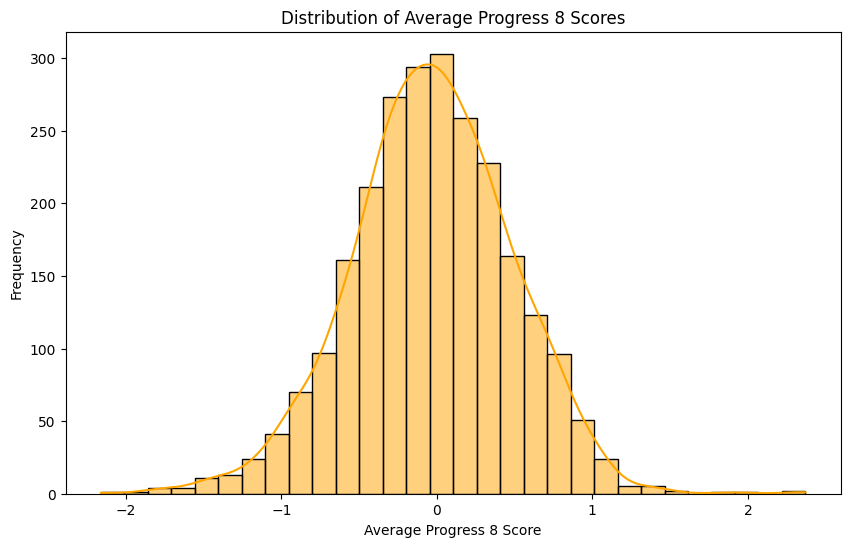
\includegraphics{P4DS_A2_Data_Analysis_Project_files/figure-pdf/cell-61-output-1.png}

\paragraph{Objective 1 Code: Analysing Gaps Between Disadvantaged and
Advantaged
Pupils}\label{objective-1-code-analysing-gaps-between-disadvantaged-and-advantaged-pupils}

I'll start by finding the mean and gaps of key performance indicators

\begin{Shaded}
\begin{Highlighting}[]
\CommentTok{\# Calculate mean scores}
\NormalTok{mean\_scores }\OperatorTok{=}\NormalTok{ \{}
    \StringTok{\textquotesingle{}Attainment 8 Disadvantaged\textquotesingle{}}\NormalTok{: merged\_df[}\StringTok{\textquotesingle{}Attainment8\_Disadvantaged\_2022\textquotesingle{}}\NormalTok{].mean(),}
    \StringTok{\textquotesingle{}Attainment 8 Non{-}Disadvantaged\textquotesingle{}}\NormalTok{: merged\_df[}\StringTok{\textquotesingle{}Average Attainment 8 score per non{-}disadvantaged pupil  {-} 2022\textquotesingle{}}\NormalTok{].mean(),}
    \StringTok{\textquotesingle{}Progress 8 Disadvantaged\textquotesingle{}}\NormalTok{: merged\_df[}\StringTok{\textquotesingle{}Progress8\_Disadvantaged\_2022\textquotesingle{}}\NormalTok{].mean(),}
    \StringTok{\textquotesingle{}Progress 8 Non{-}Disadvantaged\textquotesingle{}}\NormalTok{: merged\_df[}\StringTok{\textquotesingle{}Progress8\_NonDisadvantaged\_2022\textquotesingle{}}\NormalTok{].mean(),}
    \StringTok{\textquotesingle{}Maths Disadvantaged\textquotesingle{}}\NormalTok{: merged\_df[}\StringTok{\textquotesingle{}Progress8\_Maths\_Disadvantaged\textquotesingle{}}\NormalTok{].mean(),}
    \StringTok{\textquotesingle{}Maths Non{-}Disadvantaged\textquotesingle{}}\NormalTok{: merged\_df[}\StringTok{\textquotesingle{}Progress8\_Maths\_NonDisadvantaged\textquotesingle{}}\NormalTok{].mean(),}
    \StringTok{\textquotesingle{}English Disadvantaged\textquotesingle{}}\NormalTok{: merged\_df[}\StringTok{\textquotesingle{}Progress8\_English\_Disadvantaged\textquotesingle{}}\NormalTok{].mean(),}
    \StringTok{\textquotesingle{}English Non{-}Disadvantaged\textquotesingle{}}\NormalTok{: merged\_df[}\StringTok{\textquotesingle{}Progress8\_English\_NonDisadvantaged\textquotesingle{}}\NormalTok{].mean(),}
    \StringTok{\textquotesingle{}Percentage Disadvanted EngMaths\_95\textquotesingle{}}\NormalTok{: merged\_df[}\StringTok{\textquotesingle{}Percent\_Disadvantaged\_Strong\_Passes\textquotesingle{}}\NormalTok{].mean(),}
    \StringTok{\textquotesingle{}Percentage Nondisadv Student EngMaths\_95\textquotesingle{}}\NormalTok{: merged\_df[}\StringTok{\textquotesingle{}Percent\_Not\_Disadvantaged\_Strong\_Passes\textquotesingle{}}\NormalTok{].mean()}
\NormalTok{\}}


\NormalTok{gaps }\OperatorTok{=}\NormalTok{ \{}
    \StringTok{\textquotesingle{}Attainment 8 Gap\textquotesingle{}}\NormalTok{: merged\_df[}\StringTok{\textquotesingle{}attainment8\_gap\textquotesingle{}}\NormalTok{].mean(),}
    \StringTok{\textquotesingle{}Progress 8 Gap\textquotesingle{}}\NormalTok{: merged\_df[}\StringTok{\textquotesingle{}progress8\_gap\textquotesingle{}}\NormalTok{].mean(), }
    \StringTok{\textquotesingle{}Maths Gap\textquotesingle{}}\NormalTok{:  merged\_df[}\StringTok{\textquotesingle{}maths\_gap\textquotesingle{}}\NormalTok{].mean(),}
    \StringTok{\textquotesingle{}English Gap\textquotesingle{}}\NormalTok{:  merged\_df[}\StringTok{\textquotesingle{}english\_gap\textquotesingle{}}\NormalTok{].mean(), }
    \StringTok{\textquotesingle{}percentage\_95\textquotesingle{}}\NormalTok{:  merged\_df[}\StringTok{\textquotesingle{}5\_GCSE\_gap\textquotesingle{}}\NormalTok{].mean() }
\NormalTok{\}}

\BuiltInTok{print}\NormalTok{(}\StringTok{"}\CharTok{\textbackslash{}n}\StringTok{Mean Scores:"}\NormalTok{)}
\ControlFlowTok{for}\NormalTok{ key, value }\KeywordTok{in}\NormalTok{ mean\_scores.items():}
    \BuiltInTok{print}\NormalTok{(}\SpecialStringTok{f"}\SpecialCharTok{\{}\NormalTok{key}\SpecialCharTok{\}}\SpecialStringTok{: }\SpecialCharTok{\{}\NormalTok{value}\SpecialCharTok{:.2f\}}\SpecialStringTok{"}\NormalTok{) }\CommentTok{\#round to 2 decimal places}

\BuiltInTok{print}\NormalTok{(}\StringTok{"}\CharTok{\textbackslash{}n}\StringTok{Gaps Between Groups:"}\NormalTok{)}
\ControlFlowTok{for}\NormalTok{ key, value }\KeywordTok{in}\NormalTok{ gaps.items():}
    \BuiltInTok{print}\NormalTok{(}\SpecialStringTok{f"}\SpecialCharTok{\{}\NormalTok{key}\SpecialCharTok{\}}\SpecialStringTok{: }\SpecialCharTok{\{}\NormalTok{value}\SpecialCharTok{:.2f\}}\SpecialStringTok{"}\NormalTok{) }\CommentTok{\#round to 2 decimal places}

\end{Highlighting}
\end{Shaded}

\begin{verbatim}

Mean Scores:
Attainment 8 Disadvantaged: 40.22
Attainment 8 Non-Disadvantaged: 51.83
Progress 8 Disadvantaged: -0.47
Progress 8 Non-Disadvantaged: 0.13
Maths Disadvantaged: -0.44
Maths Non-Disadvantaged: 0.11
English Disadvantaged: -0.46
English Non-Disadvantaged: 0.12
Percentage Disadvanted EngMaths_95: 28.09
Percentage Nondisadv Student EngMaths_95: 50.01

Gaps Between Groups:
Attainment 8 Gap: 11.61
Progress 8 Gap: 0.60
Maths Gap: 0.55
English Gap: 0.58
percentage_95: 21.92
\end{verbatim}

So as to avoid repition, I will interpret the results when discussing
objectives later in this notebook. For now, it is worth noting, all the
gaps are positive, suggesting disadvantaged pupils are on average are
underperforming in every area compared to non-disadvantaged pupils

\begin{Shaded}
\begin{Highlighting}[]
\CommentTok{\# DataFrames for Progress 8 and Attainment 8}

\CommentTok{\#style}
\NormalTok{sns.}\BuiltInTok{set}\NormalTok{(style}\OperatorTok{=}\StringTok{"whitegrid"}\NormalTok{)}

\CommentTok{\# Progress 8 Performance Data}
\NormalTok{progress8\_data }\OperatorTok{=}\NormalTok{ merged\_df[[}\StringTok{\textquotesingle{}Progress8\_Disadvantaged\_2022\textquotesingle{}}\NormalTok{, }\StringTok{\textquotesingle{}Progress8\_NonDisadvantaged\_2022\textquotesingle{}}\NormalTok{]].copy()}
\NormalTok{progress8\_melted }\OperatorTok{=}\NormalTok{ progress8\_data.melt(var\_name}\OperatorTok{=}\StringTok{\textquotesingle{}Group\textquotesingle{}}\NormalTok{, value\_name}\OperatorTok{=}\StringTok{\textquotesingle{}Progress 8 Score\textquotesingle{}}\NormalTok{)}
\NormalTok{progress8\_melted[}\StringTok{\textquotesingle{}Group\textquotesingle{}}\NormalTok{] }\OperatorTok{=}\NormalTok{ progress8\_melted[}\StringTok{\textquotesingle{}Group\textquotesingle{}}\NormalTok{].}\BuiltInTok{map}\NormalTok{(\{}
    \StringTok{\textquotesingle{}Progress8\_Disadvantaged\_2022\textquotesingle{}}\NormalTok{: }\StringTok{\textquotesingle{}Disadvantaged\textquotesingle{}}\NormalTok{,}
    \StringTok{\textquotesingle{}Progress8\_NonDisadvantaged\_2022\textquotesingle{}}\NormalTok{: }\StringTok{\textquotesingle{}Non{-}Disadvantaged\textquotesingle{}}
\NormalTok{\})}

\CommentTok{\# Attainment 8 Performance Data}
\NormalTok{attainment8\_data }\OperatorTok{=}\NormalTok{ merged\_df[[}\StringTok{\textquotesingle{}Attainment8\_Disadvantaged\_2022\textquotesingle{}}\NormalTok{, }\StringTok{\textquotesingle{}Average Attainment 8 score per non{-}disadvantaged pupil  {-} 2022\textquotesingle{}}\NormalTok{]].copy()}
\NormalTok{attainment8\_melted }\OperatorTok{=}\NormalTok{ attainment8\_data.melt(var\_name}\OperatorTok{=}\StringTok{\textquotesingle{}Group\textquotesingle{}}\NormalTok{, value\_name}\OperatorTok{=}\StringTok{\textquotesingle{}Attainment 8 Score\textquotesingle{}}\NormalTok{)}
\NormalTok{attainment8\_melted[}\StringTok{\textquotesingle{}Group\textquotesingle{}}\NormalTok{] }\OperatorTok{=}\NormalTok{ attainment8\_melted[}\StringTok{\textquotesingle{}Group\textquotesingle{}}\NormalTok{].}\BuiltInTok{map}\NormalTok{(\{}
    \StringTok{\textquotesingle{}Attainment8\_Disadvantaged\_2022\textquotesingle{}}\NormalTok{: }\StringTok{\textquotesingle{}Disadvantaged\textquotesingle{}}\NormalTok{,}
    \StringTok{\textquotesingle{}Average Attainment 8 score per non{-}disadvantaged pupil  {-} 2022\textquotesingle{}}\NormalTok{: }\StringTok{\textquotesingle{}Non{-}Disadvantaged\textquotesingle{}}
\NormalTok{\})}


\NormalTok{fig, axes }\OperatorTok{=}\NormalTok{ plt.subplots(}\DecValTok{1}\NormalTok{, }\DecValTok{2}\NormalTok{, figsize}\OperatorTok{=}\NormalTok{(}\DecValTok{16}\NormalTok{, }\DecValTok{8}\NormalTok{))}

\CommentTok{\# Box Plot for Progress 8 Scores}
\NormalTok{sns.boxplot(}
\NormalTok{    x}\OperatorTok{=}\StringTok{\textquotesingle{}Group\textquotesingle{}}\NormalTok{,}
\NormalTok{    y}\OperatorTok{=}\StringTok{\textquotesingle{}Progress 8 Score\textquotesingle{}}\NormalTok{,}
\NormalTok{    data}\OperatorTok{=}\NormalTok{progress8\_melted,}
\NormalTok{    palette}\OperatorTok{=}\StringTok{"Set1"}\NormalTok{,}
\NormalTok{    ax}\OperatorTok{=}\NormalTok{axes[}\DecValTok{0}\NormalTok{]}
\NormalTok{)}
\NormalTok{axes[}\DecValTok{0}\NormalTok{].set\_title(}\StringTok{\textquotesingle{}Progress 8 Scores by Group\textquotesingle{}}\NormalTok{, fontsize}\OperatorTok{=}\DecValTok{16}\NormalTok{)}
\NormalTok{axes[}\DecValTok{0}\NormalTok{].set\_xlabel(}\StringTok{\textquotesingle{}Group\textquotesingle{}}\NormalTok{, fontsize}\OperatorTok{=}\DecValTok{14}\NormalTok{)}
\NormalTok{axes[}\DecValTok{0}\NormalTok{].set\_ylabel(}\StringTok{\textquotesingle{}Progress 8 Score\textquotesingle{}}\NormalTok{, fontsize}\OperatorTok{=}\DecValTok{14}\NormalTok{)}

\CommentTok{\# Box Plot for Attainment 8 Scores}
\NormalTok{sns.boxplot(}
\NormalTok{    x}\OperatorTok{=}\StringTok{\textquotesingle{}Group\textquotesingle{}}\NormalTok{,}
\NormalTok{    y}\OperatorTok{=}\StringTok{\textquotesingle{}Attainment 8 Score\textquotesingle{}}\NormalTok{,}
\NormalTok{    data}\OperatorTok{=}\NormalTok{attainment8\_melted,}
\NormalTok{    palette}\OperatorTok{=}\StringTok{"Set2"}\NormalTok{,}
\NormalTok{    ax}\OperatorTok{=}\NormalTok{axes[}\DecValTok{1}\NormalTok{]}
\NormalTok{)}
\NormalTok{axes[}\DecValTok{1}\NormalTok{].set\_title(}\StringTok{\textquotesingle{}Attainment 8 Scores by Group\textquotesingle{}}\NormalTok{, fontsize}\OperatorTok{=}\DecValTok{16}\NormalTok{)}
\NormalTok{axes[}\DecValTok{1}\NormalTok{].set\_xlabel(}\StringTok{\textquotesingle{}Group\textquotesingle{}}\NormalTok{, fontsize}\OperatorTok{=}\DecValTok{14}\NormalTok{)}
\NormalTok{axes[}\DecValTok{1}\NormalTok{].set\_ylabel(}\StringTok{\textquotesingle{}Attainment 8 Score\textquotesingle{}}\NormalTok{, fontsize}\OperatorTok{=}\DecValTok{14}\NormalTok{)}
\NormalTok{plt.tight\_layout() }\CommentTok{\#adjust plot for better fit}

\CommentTok{\#save the file to the images folder}
\NormalTok{images\_dir }\OperatorTok{=} \StringTok{\textquotesingle{}images\textquotesingle{}}
\NormalTok{image\_path }\OperatorTok{=}\NormalTok{ os.path.join(images\_dir,}\StringTok{\textquotesingle{}obj1\_progress8\_attainment8\_boxplot.png\textquotesingle{}}\NormalTok{ )}
\NormalTok{plt.savefig(image\_path)}

\NormalTok{plt.show()}
\end{Highlighting}
\end{Shaded}

\begin{verbatim}
C:\Users\saqib\AppData\Local\Temp\ipykernel_37860\2793708818.py:26: FutureWarning: 

Passing `palette` without assigning `hue` is deprecated and will be removed in v0.14.0. Assign the `x` variable to `hue` and set `legend=False` for the same effect.

  sns.boxplot(
C:\Users\saqib\AppData\Local\Temp\ipykernel_37860\2793708818.py:38: FutureWarning: 

Passing `palette` without assigning `hue` is deprecated and will be removed in v0.14.0. Assign the `x` variable to `hue` and set `legend=False` for the same effect.

  sns.boxplot(
\end{verbatim}

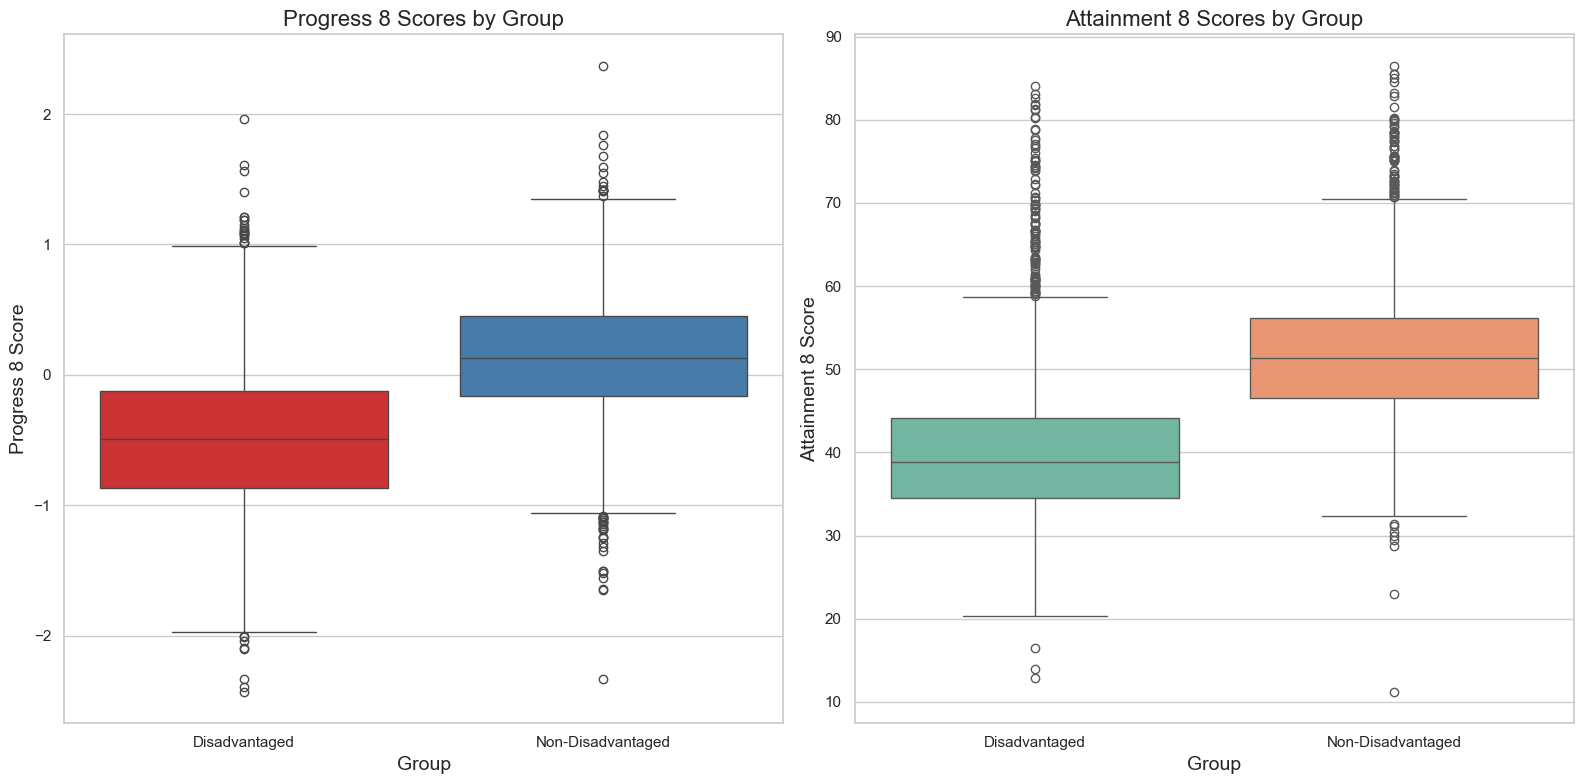
\includegraphics{P4DS_A2_Data_Analysis_Project_files/figure-pdf/cell-63-output-2.png}

\begin{Shaded}
\begin{Highlighting}[]
\CommentTok{\# Calculate summary statistics for Attainment 8 Scores}
\NormalTok{attainment8\_grouped }\OperatorTok{=}\NormalTok{ attainment8\_melted.groupby(}\StringTok{\textquotesingle{}Group\textquotesingle{}}\NormalTok{)[}\StringTok{\textquotesingle{}Attainment 8 Score\textquotesingle{}}\NormalTok{]}

\CommentTok{\# Calculate statistics for Attainment 8}
\NormalTok{attainment8\_stats }\OperatorTok{=}\NormalTok{ attainment8\_grouped.describe()}
\NormalTok{attainment8\_q1 }\OperatorTok{=}\NormalTok{ attainment8\_grouped.quantile(}\FloatTok{0.25}\NormalTok{)}
\NormalTok{attainment8\_q3 }\OperatorTok{=}\NormalTok{ attainment8\_grouped.quantile(}\FloatTok{0.75}\NormalTok{)}
\NormalTok{attainment8\_iqr }\OperatorTok{=}\NormalTok{ attainment8\_q3 }\OperatorTok{{-}}\NormalTok{ attainment8\_q1}
\NormalTok{attainment8\_range }\OperatorTok{=}\NormalTok{ attainment8\_grouped.}\BuiltInTok{max}\NormalTok{() }\OperatorTok{{-}}\NormalTok{ attainment8\_grouped.}\BuiltInTok{min}\NormalTok{()}
\NormalTok{attainment8\_median }\OperatorTok{=}\NormalTok{ attainment8\_grouped.median()}
\NormalTok{attainment8\_min }\OperatorTok{=}\NormalTok{ attainment8\_grouped.}\BuiltInTok{min}\NormalTok{()}
\NormalTok{attainment8\_max }\OperatorTok{=}\NormalTok{ attainment8\_grouped.}\BuiltInTok{max}\NormalTok{()}

\CommentTok{\#}
\NormalTok{attainment8\_summary }\OperatorTok{=}\NormalTok{ pd.DataFrame(\{}
    \StringTok{\textquotesingle{}Median\textquotesingle{}}\NormalTok{: attainment8\_median,}
    \StringTok{\textquotesingle{}Q1 (25\%)\textquotesingle{}}\NormalTok{: attainment8\_q1,}
    \StringTok{\textquotesingle{}Q3 (75\%)\textquotesingle{}}\NormalTok{: attainment8\_q3,}
    \StringTok{\textquotesingle{}IQR\textquotesingle{}}\NormalTok{: attainment8\_iqr,}
    \StringTok{\textquotesingle{}Min\textquotesingle{}}\NormalTok{: attainment8\_min,}
    \StringTok{\textquotesingle{}Max\textquotesingle{}}\NormalTok{: attainment8\_max,}
    \StringTok{\textquotesingle{}Range\textquotesingle{}}\NormalTok{: attainment8\_range}
\NormalTok{\})}

\BuiltInTok{print}\NormalTok{(}\StringTok{"}\CharTok{\textbackslash{}n}\StringTok{Attainment 8 Scores Summary:"}\NormalTok{)}
\BuiltInTok{print}\NormalTok{(attainment8\_summary)}


\CommentTok{\# Calculate summary statistics for Progress 8 Scores}


\NormalTok{progress8\_grouped }\OperatorTok{=}\NormalTok{ progress8\_melted.groupby(}\StringTok{\textquotesingle{}Group\textquotesingle{}}\NormalTok{)[}\StringTok{\textquotesingle{}Progress 8 Score\textquotesingle{}}\NormalTok{]}

\CommentTok{\# Calculate statistics for Progress 8}
\NormalTok{progress8\_stats }\OperatorTok{=}\NormalTok{ progress8\_grouped.describe()}
\NormalTok{progress8\_q1 }\OperatorTok{=}\NormalTok{ progress8\_grouped.quantile(}\FloatTok{0.25}\NormalTok{)}
\NormalTok{progress8\_q3 }\OperatorTok{=}\NormalTok{ progress8\_grouped.quantile(}\FloatTok{0.75}\NormalTok{)}
\NormalTok{progress8\_iqr }\OperatorTok{=}\NormalTok{ progress8\_q3 }\OperatorTok{{-}}\NormalTok{ progress8\_q1}
\NormalTok{progress8\_range }\OperatorTok{=}\NormalTok{ progress8\_grouped.}\BuiltInTok{max}\NormalTok{() }\OperatorTok{{-}}\NormalTok{ progress8\_grouped.}\BuiltInTok{min}\NormalTok{()}
\NormalTok{progress8\_median }\OperatorTok{=}\NormalTok{ progress8\_grouped.median()}
\NormalTok{progress8\_min }\OperatorTok{=}\NormalTok{ progress8\_grouped.}\BuiltInTok{min}\NormalTok{()}
\NormalTok{progress8\_max }\OperatorTok{=}\NormalTok{ progress8\_grouped.}\BuiltInTok{max}\NormalTok{()}


\NormalTok{progress8\_summary }\OperatorTok{=}\NormalTok{ pd.DataFrame(\{}
    \StringTok{\textquotesingle{}Median\textquotesingle{}}\NormalTok{: progress8\_median,}
    \StringTok{\textquotesingle{}Q1 (25\%)\textquotesingle{}}\NormalTok{: progress8\_q1,}
    \StringTok{\textquotesingle{}Q3 (75\%)\textquotesingle{}}\NormalTok{: progress8\_q3,}
    \StringTok{\textquotesingle{}IQR\textquotesingle{}}\NormalTok{: progress8\_iqr,}
    \StringTok{\textquotesingle{}Min\textquotesingle{}}\NormalTok{: progress8\_min,}
    \StringTok{\textquotesingle{}Max\textquotesingle{}}\NormalTok{: progress8\_max,}
    \StringTok{\textquotesingle{}Range\textquotesingle{}}\NormalTok{: progress8\_range}
\NormalTok{\})}


\BuiltInTok{print}\NormalTok{(}\StringTok{"}\CharTok{\textbackslash{}n}\StringTok{Progress 8 Scores Summary:"}\NormalTok{)}
\BuiltInTok{print}\NormalTok{(progress8\_summary)}
\end{Highlighting}
\end{Shaded}

\begin{verbatim}

Attainment 8 Scores Summary:
                   Median  Q1 (25%)  Q3 (75%)  IQR   Min   Max  Range
Group                                                                
Disadvantaged        38.8      34.5      44.2  9.7  12.9  84.1   71.2
Non-Disadvantaged    51.3      46.6      56.2  9.6  11.2  86.5   75.3

Progress 8 Scores Summary:
                   Median  Q1 (25%)  Q3 (75%)   IQR   Min   Max  Range
Group                                                                 
Disadvantaged       -0.49     -0.87     -0.12  0.75 -2.43  1.96   4.39
Non-Disadvantaged    0.13     -0.16      0.45  0.61 -2.33  2.37   4.70
\end{verbatim}

\begin{Shaded}
\begin{Highlighting}[]
\CommentTok{\# Dataframes for Maths and English}

\CommentTok{\# Style}
\NormalTok{sns.}\BuiltInTok{set}\NormalTok{(style}\OperatorTok{=}\StringTok{"whitegrid"}\NormalTok{)}

\CommentTok{\# Maths Performance Data}
\NormalTok{maths\_data }\OperatorTok{=}\NormalTok{ merged\_df[[}\StringTok{\textquotesingle{}Progress8\_Maths\_Disadvantaged\textquotesingle{}}\NormalTok{, }\StringTok{\textquotesingle{}Progress8\_Maths\_NonDisadvantaged\textquotesingle{}}\NormalTok{]].copy()}
\NormalTok{maths\_melted }\OperatorTok{=}\NormalTok{ maths\_data.melt(var\_name}\OperatorTok{=}\StringTok{\textquotesingle{}Group\textquotesingle{}}\NormalTok{, value\_name}\OperatorTok{=}\StringTok{\textquotesingle{}Maths Score\textquotesingle{}}\NormalTok{)}
\NormalTok{maths\_melted[}\StringTok{\textquotesingle{}Group\textquotesingle{}}\NormalTok{] }\OperatorTok{=}\NormalTok{ maths\_melted[}\StringTok{\textquotesingle{}Group\textquotesingle{}}\NormalTok{].}\BuiltInTok{map}\NormalTok{(\{}
    \StringTok{\textquotesingle{}Progress8\_Maths\_Disadvantaged\textquotesingle{}}\NormalTok{: }\StringTok{\textquotesingle{}Disadvantaged\textquotesingle{}}\NormalTok{,}
    \StringTok{\textquotesingle{}Progress8\_Maths\_NonDisadvantaged\textquotesingle{}}\NormalTok{: }\StringTok{\textquotesingle{}Non{-}Disadvantaged\textquotesingle{}}
\NormalTok{\})}

\CommentTok{\# English Performance Data}
\NormalTok{english\_data }\OperatorTok{=}\NormalTok{ merged\_df[[}\StringTok{\textquotesingle{}Progress8\_English\_Disadvantaged\textquotesingle{}}\NormalTok{, }\StringTok{\textquotesingle{}Progress8\_English\_NonDisadvantaged\textquotesingle{}}\NormalTok{]].copy()}
\NormalTok{english\_melted }\OperatorTok{=}\NormalTok{ english\_data.melt(var\_name}\OperatorTok{=}\StringTok{\textquotesingle{}Group\textquotesingle{}}\NormalTok{, value\_name}\OperatorTok{=}\StringTok{\textquotesingle{}English Score\textquotesingle{}}\NormalTok{)}
\NormalTok{english\_melted[}\StringTok{\textquotesingle{}Group\textquotesingle{}}\NormalTok{] }\OperatorTok{=}\NormalTok{ english\_melted[}\StringTok{\textquotesingle{}Group\textquotesingle{}}\NormalTok{].}\BuiltInTok{map}\NormalTok{(\{}
    \StringTok{\textquotesingle{}Progress8\_English\_Disadvantaged\textquotesingle{}}\NormalTok{: }\StringTok{\textquotesingle{}Disadvantaged\textquotesingle{}}\NormalTok{,}
    \StringTok{\textquotesingle{}Progress8\_English\_NonDisadvantaged\textquotesingle{}}\NormalTok{: }\StringTok{\textquotesingle{}Non{-}Disadvantaged\textquotesingle{}}
\NormalTok{\})}


\NormalTok{fig, axes }\OperatorTok{=}\NormalTok{ plt.subplots(}\DecValTok{1}\NormalTok{, }\DecValTok{2}\NormalTok{, figsize}\OperatorTok{=}\NormalTok{(}\DecValTok{16}\NormalTok{, }\DecValTok{8}\NormalTok{))}

\CommentTok{\# Box Plot for Maths Scores}
\NormalTok{sns.boxplot(}
\NormalTok{    x}\OperatorTok{=}\StringTok{\textquotesingle{}Group\textquotesingle{}}\NormalTok{,}
\NormalTok{    y}\OperatorTok{=}\StringTok{\textquotesingle{}Maths Score\textquotesingle{}}\NormalTok{,}
\NormalTok{    data}\OperatorTok{=}\NormalTok{maths\_melted,}
\NormalTok{    palette}\OperatorTok{=}\StringTok{"Set2"}\NormalTok{,}
\NormalTok{    ax}\OperatorTok{=}\NormalTok{axes[}\DecValTok{0}\NormalTok{]}
\NormalTok{)}
\NormalTok{axes[}\DecValTok{0}\NormalTok{].set\_title(}\StringTok{\textquotesingle{}Maths Scores by Group\textquotesingle{}}\NormalTok{, fontsize}\OperatorTok{=}\DecValTok{16}\NormalTok{)}
\NormalTok{axes[}\DecValTok{0}\NormalTok{].set\_xlabel(}\StringTok{\textquotesingle{}Group\textquotesingle{}}\NormalTok{, fontsize}\OperatorTok{=}\DecValTok{14}\NormalTok{)}
\NormalTok{axes[}\DecValTok{0}\NormalTok{].set\_ylabel(}\StringTok{\textquotesingle{}Maths Score\textquotesingle{}}\NormalTok{, fontsize}\OperatorTok{=}\DecValTok{14}\NormalTok{)}


\CommentTok{\# Box Plot for English Scores}
\NormalTok{sns.boxplot(}
\NormalTok{    x}\OperatorTok{=}\StringTok{\textquotesingle{}Group\textquotesingle{}}\NormalTok{,}
\NormalTok{    y}\OperatorTok{=}\StringTok{\textquotesingle{}English Score\textquotesingle{}}\NormalTok{,}
\NormalTok{    data}\OperatorTok{=}\NormalTok{english\_melted,}
\NormalTok{    palette}\OperatorTok{=}\StringTok{"Set3"}\NormalTok{,}
\NormalTok{    ax}\OperatorTok{=}\NormalTok{axes[}\DecValTok{1}\NormalTok{]}
\NormalTok{)}
\NormalTok{axes[}\DecValTok{1}\NormalTok{].set\_title(}\StringTok{\textquotesingle{}English Scores by Group\textquotesingle{}}\NormalTok{, fontsize}\OperatorTok{=}\DecValTok{16}\NormalTok{)}
\NormalTok{axes[}\DecValTok{1}\NormalTok{].set\_xlabel(}\StringTok{\textquotesingle{}Group\textquotesingle{}}\NormalTok{, fontsize}\OperatorTok{=}\DecValTok{14}\NormalTok{)}
\NormalTok{axes[}\DecValTok{1}\NormalTok{].set\_ylabel(}\StringTok{\textquotesingle{}English Score\textquotesingle{}}\NormalTok{, fontsize}\OperatorTok{=}\DecValTok{14}\NormalTok{)}
\NormalTok{plt.tight\_layout() }\CommentTok{\# Adjust layout for better fit}

\CommentTok{\# Save the combined box plots as a PNG file in images folder }

\NormalTok{images\_dir }\OperatorTok{=} \StringTok{\textquotesingle{}images\textquotesingle{}}
\NormalTok{image\_path }\OperatorTok{=}\NormalTok{ os.path.join(images\_dir,}\StringTok{\textquotesingle{}obj1\_maths\_english\_scores\_boxplot.png\textquotesingle{}}\NormalTok{)}
\NormalTok{plt.savefig(image\_path)}


\NormalTok{plt.show()}
\end{Highlighting}
\end{Shaded}

\begin{verbatim}
C:\Users\saqib\AppData\Local\Temp\ipykernel_37860\367155346.py:26: FutureWarning: 

Passing `palette` without assigning `hue` is deprecated and will be removed in v0.14.0. Assign the `x` variable to `hue` and set `legend=False` for the same effect.

  sns.boxplot(
C:\Users\saqib\AppData\Local\Temp\ipykernel_37860\367155346.py:39: FutureWarning: 

Passing `palette` without assigning `hue` is deprecated and will be removed in v0.14.0. Assign the `x` variable to `hue` and set `legend=False` for the same effect.

  sns.boxplot(
\end{verbatim}

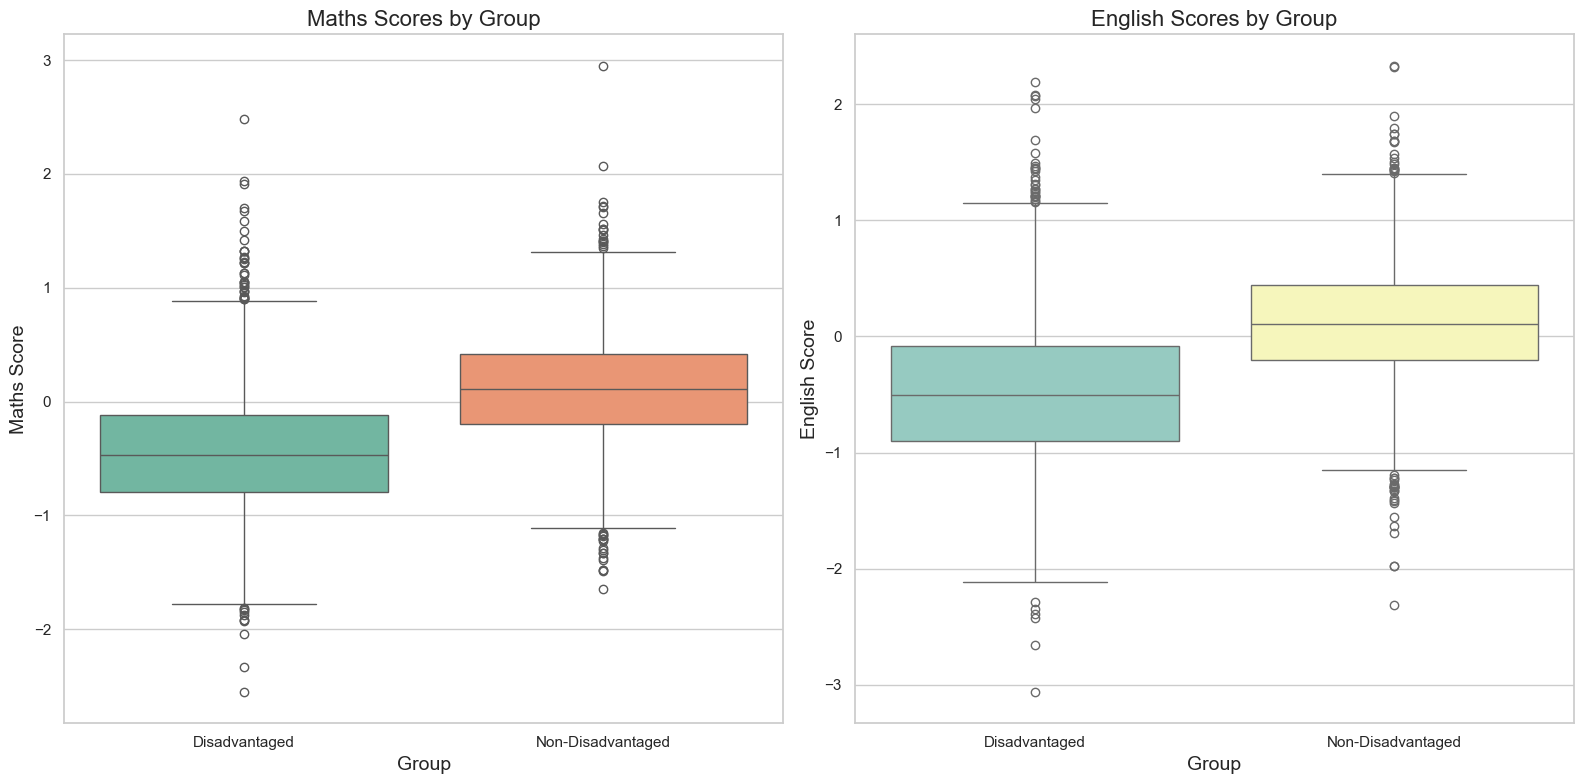
\includegraphics{P4DS_A2_Data_Analysis_Project_files/figure-pdf/cell-65-output-2.png}

\begin{Shaded}
\begin{Highlighting}[]
\CommentTok{\# Calculate summary statistics for Maths Scores}

\NormalTok{maths\_grouped }\OperatorTok{=}\NormalTok{ maths\_melted.groupby(}\StringTok{\textquotesingle{}Group\textquotesingle{}}\NormalTok{)[}\StringTok{\textquotesingle{}Maths Score\textquotesingle{}}\NormalTok{]}

\CommentTok{\# Calculate statistics for Maths}
\NormalTok{maths\_stats }\OperatorTok{=}\NormalTok{ maths\_grouped.describe()}
\NormalTok{maths\_q1 }\OperatorTok{=}\NormalTok{ maths\_grouped.quantile(}\FloatTok{0.25}\NormalTok{)}
\NormalTok{maths\_q3 }\OperatorTok{=}\NormalTok{ maths\_grouped.quantile(}\FloatTok{0.75}\NormalTok{)}
\NormalTok{maths\_iqr }\OperatorTok{=}\NormalTok{ maths\_q3 }\OperatorTok{{-}}\NormalTok{ maths\_q1}
\NormalTok{maths\_range }\OperatorTok{=}\NormalTok{ maths\_grouped.}\BuiltInTok{max}\NormalTok{() }\OperatorTok{{-}}\NormalTok{ maths\_grouped.}\BuiltInTok{min}\NormalTok{()}
\NormalTok{maths\_median }\OperatorTok{=}\NormalTok{ maths\_grouped.median()}
\NormalTok{maths\_min }\OperatorTok{=}\NormalTok{ maths\_grouped.}\BuiltInTok{min}\NormalTok{()}
\NormalTok{maths\_max }\OperatorTok{=}\NormalTok{ maths\_grouped.}\BuiltInTok{max}\NormalTok{()}


\NormalTok{maths\_summary }\OperatorTok{=}\NormalTok{ pd.DataFrame(\{}
    \StringTok{\textquotesingle{}Median\textquotesingle{}}\NormalTok{: maths\_median,}
    \StringTok{\textquotesingle{}Q1 (25\%)\textquotesingle{}}\NormalTok{: maths\_q1,}
    \StringTok{\textquotesingle{}Q3 (75\%)\textquotesingle{}}\NormalTok{: maths\_q3,}
    \StringTok{\textquotesingle{}IQR\textquotesingle{}}\NormalTok{: maths\_iqr,}
    \StringTok{\textquotesingle{}Min\textquotesingle{}}\NormalTok{: maths\_min,}
    \StringTok{\textquotesingle{}Max\textquotesingle{}}\NormalTok{: maths\_max,}
    \StringTok{\textquotesingle{}Range\textquotesingle{}}\NormalTok{: maths\_range}
\NormalTok{\})}


\BuiltInTok{print}\NormalTok{(}\StringTok{"}\CharTok{\textbackslash{}n}\StringTok{Maths Scores Summary:"}\NormalTok{)}
\BuiltInTok{print}\NormalTok{(maths\_summary)}


\CommentTok{\# Calculate summary statistics for English Scores}


\NormalTok{english\_grouped }\OperatorTok{=}\NormalTok{ english\_melted.groupby(}\StringTok{\textquotesingle{}Group\textquotesingle{}}\NormalTok{)[}\StringTok{\textquotesingle{}English Score\textquotesingle{}}\NormalTok{]}

\NormalTok{english\_stats }\OperatorTok{=}\NormalTok{ english\_grouped.describe()}
\NormalTok{english\_q1 }\OperatorTok{=}\NormalTok{ english\_grouped.quantile(}\FloatTok{0.25}\NormalTok{)}
\NormalTok{english\_q3 }\OperatorTok{=}\NormalTok{ english\_grouped.quantile(}\FloatTok{0.75}\NormalTok{)}
\NormalTok{english\_iqr }\OperatorTok{=}\NormalTok{ english\_q3 }\OperatorTok{{-}}\NormalTok{ english\_q1}
\NormalTok{english\_range }\OperatorTok{=}\NormalTok{ english\_grouped.}\BuiltInTok{max}\NormalTok{() }\OperatorTok{{-}}\NormalTok{ english\_grouped.}\BuiltInTok{min}\NormalTok{()}
\NormalTok{english\_median }\OperatorTok{=}\NormalTok{ english\_grouped.median()}
\NormalTok{english\_min }\OperatorTok{=}\NormalTok{ english\_grouped.}\BuiltInTok{min}\NormalTok{()}
\NormalTok{english\_max }\OperatorTok{=}\NormalTok{ english\_grouped.}\BuiltInTok{max}\NormalTok{()}


\NormalTok{english\_summary }\OperatorTok{=}\NormalTok{ pd.DataFrame(\{}
    \StringTok{\textquotesingle{}Median\textquotesingle{}}\NormalTok{: english\_median,}
    \StringTok{\textquotesingle{}Q1 (25\%)\textquotesingle{}}\NormalTok{: english\_q1,}
    \StringTok{\textquotesingle{}Q3 (75\%)\textquotesingle{}}\NormalTok{: english\_q3,}
    \StringTok{\textquotesingle{}IQR\textquotesingle{}}\NormalTok{: english\_iqr,}
    \StringTok{\textquotesingle{}Min\textquotesingle{}}\NormalTok{: english\_min,}
    \StringTok{\textquotesingle{}Max\textquotesingle{}}\NormalTok{: english\_max,}
    \StringTok{\textquotesingle{}Range\textquotesingle{}}\NormalTok{: english\_range}
\NormalTok{\})}


\BuiltInTok{print}\NormalTok{(}\StringTok{"}\CharTok{\textbackslash{}n}\StringTok{English Scores Summary:"}\NormalTok{)}
\BuiltInTok{print}\NormalTok{(english\_summary)}
\end{Highlighting}
\end{Shaded}

\begin{verbatim}

Maths Scores Summary:
                   Median  Q1 (25%)  Q3 (75%)   IQR   Min   Max  Range
Group                                                                 
Disadvantaged       -0.47     -0.79     -0.12  0.67 -2.55  2.48   5.03
Non-Disadvantaged    0.11     -0.20      0.42  0.62 -1.65  2.95   4.60

English Scores Summary:
                   Median  Q1 (25%)  Q3 (75%)   IQR   Min   Max  Range
Group                                                                 
Disadvantaged       -0.50      -0.9     -0.08  0.82 -3.06  2.19   5.25
Non-Disadvantaged    0.11      -0.2      0.44  0.64 -2.31  2.33   4.64
\end{verbatim}

\paragraph{Objective 2 Code: Identify and Analyse Outlier Schools in
Positive Progress 8 of Disadavantaged
Pupils}\label{objective-2-code-identify-and-analyse-outlier-schools-in-positive-progress-8-of-disadavantaged-pupils}

For simplicity, I have chosen to use the Interquarticle Range approach
to identify outliers, rather than Z-score. This also allows for easier
visualisation using a boxplot. I will begin by establishing quartiles
for a box plot to see the distribtion of progress-8 disadvantaged
students and then determine outliers using standard approach of
interquartile range. As I am interested in high performing schools, I
will only take the positive outlier schools

\begin{Shaded}
\begin{Highlighting}[]
\NormalTok{merged\_df\_2}\OperatorTok{=}\NormalTok{ merged\_df.copy() }\CommentTok{\# copy of merged\_df is used for data integrity}
\NormalTok{merged\_df\_2.head()}
\end{Highlighting}
\end{Shaded}

\begin{longtable}[]{@{}llllllllllllllllllllll@{}}
\toprule\noalign{}
& URN & Local\_Authority\_Name & Local\_Authority\_Number & School\_Type
& School\_College\_Type & Religious\_Character & Admissions\_Policy &
School\_Gender & Ofsted\_Rating & School postcode & ... & NaN & Index of
Multiple Deprivation Decile & LSOA Name & POSTCODE & progress8\_gap &
attainment8\_gap & maths\_gap & english\_gap & 5\_GCSE\_gap &
pupilpremium\_per\_pupil \\
\midrule\noalign{}
\endhead
\bottomrule\noalign{}
\endlastfoot
207 & 105135 & Greenwich & 203 & Academy sponsor led & Academy & Roman
Catholic & Non-selective & Mixed & Requires improvement & SE2 9PX & ...
& NaN & 2.0 & Greenwich 003E E01001579 & SE2 9PX & 0.48 & 6.9 & 0.51 &
0.69 & 12.0 & 985.0 \\
718 & 129342 & Solihull & 334 & Academy sponsor led & Academy & Does not
apply & Non-selective & Mixed & Good & B37 5JS & ... & NaN & 3.0 &
Solihull 007D E01010144 & B37 5JS & 0.59 & 6.3 & 0.40 & 0.91 & 30.0 &
985.0 \\
722 & 130247 & Reading & 870 & Academy sponsor led & Academy & Does not
apply & Non-selective & Mixed & Serious Weaknesses & RG2 8AF & ... & NaN
& 2.0 & Reading 017D E01016438 & RG2 8AF & 0.90 & 15.3 & 0.50 & 0.41 &
12.0 & 985.0 \\
723 & 130908 & Middlesbrough & 806 & Academy sponsor led & Academy &
Does not apply & Non-selective & Mixed & Good & TS5 4AG & ... & NaN &
2.0 & Middlesbrough 008D E01012014 & TS5 4AG & 0.62 & 10.9 & 0.78 & 0.62
& 32.0 & 985.0 \\
724 & 130909 & Bradford & 380 & Academy sponsor led & Academy & Does not
apply & Non-selective & Mixed & Outstanding & BD5 7RR & ... & 202223.0 &
1.0 & Bradford 048B E01010732 & BD5 7RR & 0.49 & 8.4 & 0.25 & 0.40 &
10.0 & 985.0 \\
\end{longtable}

\begin{Shaded}
\begin{Highlighting}[]
\CommentTok{\#  Outlier detection of schools in progress 8 performance of disadavantaged pupils}

\NormalTok{Q1 }\OperatorTok{=}\NormalTok{ merged\_df\_2[}\StringTok{\textquotesingle{}Progress8\_Disadvantaged\_2022\textquotesingle{}}\NormalTok{].quantile(}\FloatTok{0.25}\NormalTok{)}
\NormalTok{Q3 }\OperatorTok{=}\NormalTok{ merged\_df\_2[}\StringTok{\textquotesingle{}Progress8\_Disadvantaged\_2022\textquotesingle{}}\NormalTok{].quantile(}\FloatTok{0.75}\NormalTok{)}
\NormalTok{IQR }\OperatorTok{=}\NormalTok{ Q3 }\OperatorTok{{-}}\NormalTok{ Q1}
\NormalTok{lower\_bound }\OperatorTok{=}\NormalTok{ Q1 }\OperatorTok{{-}} \FloatTok{1.5} \OperatorTok{*}\NormalTok{ IQR}
\NormalTok{upper\_bound }\OperatorTok{=}\NormalTok{ Q3 }\OperatorTok{+} \FloatTok{1.5} \OperatorTok{*}\NormalTok{ IQR}
 \CommentTok{\# only upper bound is taken as we are interested in high{-}performing schools}
\NormalTok{outliers\_p8\_disadv }\OperatorTok{=}\NormalTok{ merged\_df\_2[(merged\_df\_2[}\StringTok{\textquotesingle{}Progress8\_Disadvantaged\_2022\textquotesingle{}}\NormalTok{] }\OperatorTok{\textgreater{}}\NormalTok{ upper\_bound)]  }
\NormalTok{outliers\_p8\_disadv[[}\StringTok{\textquotesingle{}School\_Name\textquotesingle{}}\NormalTok{,}\StringTok{\textquotesingle{}Trust\_Name\textquotesingle{}}\NormalTok{,}\StringTok{\textquotesingle{}Progress8\_Disadvantaged\_2022\textquotesingle{}}\NormalTok{]].sort\_values(}\StringTok{\textquotesingle{}Progress8\_Disadvantaged\_2022\textquotesingle{}}\NormalTok{, ascending}\OperatorTok{=}\VariableTok{False}\NormalTok{)}
\end{Highlighting}
\end{Shaded}

\begin{longtable}[]{@{}llll@{}}
\toprule\noalign{}
& School\_Name & Trust\_Name & Progress8\_Disadvantaged\_2022 \\
\midrule\noalign{}
\endhead
\bottomrule\noalign{}
\endlastfoot
2699 & Michaela Community School & MICHAELA COMMUNITY SCHOOLS TRUST &
1.96 \\
3545 & St Peter\textquotesingle s Catholic School & XAVIER CATHOLIC
EDUCATION TRUST & 1.61 \\
2826 & Tauheedul Islam Girls\textquotesingle{} High School & STAR
ACADEMIES & 1.56 \\
3528 & Eden Girls\textquotesingle{} Leadership Academy, Birmingham &
STAR ACADEMIES & 1.40 \\
2058 & St Mark\textquotesingle s Catholic School & THE DIOCESE OF
WESTMINSTER ACADEMY TRUST & 1.21 \\
2368 & Sacred Heart Catholic School & SACRED HEART CATHOLIC SCHOOL &
1.21 \\
2830 & The Hurlingham Academy & UNITED LEARNING TRUST & 1.19 \\
2981 & Ealing Fields High School & TWYFORD CHURCH OF ENGLAND ACADEMIES
TRUST & 1.19 \\
2884 & Eden Boys\textquotesingle{} School, Preston & STAR ACADEMIES &
1.15 \\
3530 & St Francis Xavier School - a Joint Catholic an... & NICHOLAS
POSTGATE CATHOLIC ACADEMY TRUST & 1.13 \\
2950 & Bolton Muslim Girls School & PROSPER MULTI ACADEMY TRUST &
1.11 \\
1475 & Birmingham Ormiston Academy & BIRMINGHAM ORMISTON ACADEMY &
1.10 \\
3158 & Dartford Grammar School for Girls & THE ARETÉ TRUST & 1.09 \\
1120 & Lancaster Girls\textquotesingle{} Grammar School & LANCASTER
GIRLS\textquotesingle{} GRAMMAR SCHOOL & 1.09 \\
833 & Ashcroft Technology Academy & PROSPECT EDUCATION (TECHNOLOGY)
TRUST LIMITED & 1.09 \\
2162 & Ark Bolingbroke Academy & ARK SCHOOLS & 1.07 \\
1279 & Wilson\textquotesingle s School & WILSON\textquotesingle S SCHOOL
& 1.07 \\
1919 & Featherstone High School & GRAND UNION MULTI ACADEMY TRUST &
1.05 \\
849 & Wren Academy Finchley & WREN ACADEMIES TRUST & 1.02 \\
1645 & Bentley Wood High School & THE BENTLEY WOOD TRUST & 1.01 \\
2264 & Nishkam High School & NISHKAM SCHOOL TRUST & 1.01 \\
\end{longtable}

Similarly, I will repear the process for non-disadvantaged pupils'
progress-8 score

\begin{Shaded}
\begin{Highlighting}[]
\NormalTok{Q1 }\OperatorTok{=}\NormalTok{ merged\_df\_2[}\StringTok{\textquotesingle{}Progress8\_NonDisadvantaged\_2022\textquotesingle{}}\NormalTok{].quantile(}\FloatTok{0.25}\NormalTok{)}
\NormalTok{Q3 }\OperatorTok{=}\NormalTok{ merged\_df\_2[}\StringTok{\textquotesingle{}Progress8\_NonDisadvantaged\_2022\textquotesingle{}}\NormalTok{].quantile(}\FloatTok{0.75}\NormalTok{)}
\NormalTok{IQR }\OperatorTok{=}\NormalTok{ Q3 }\OperatorTok{{-}}\NormalTok{ Q1}
\NormalTok{lower\_bound }\OperatorTok{=}\NormalTok{ Q1 }\OperatorTok{{-}} \FloatTok{1.5} \OperatorTok{*}\NormalTok{ IQR}
\NormalTok{upper\_bound }\OperatorTok{=}\NormalTok{ Q3 }\OperatorTok{+} \FloatTok{1.5} \OperatorTok{*}\NormalTok{ IQR}
\NormalTok{outliers\_p8\_adv }\OperatorTok{=}\NormalTok{ merged\_df\_2[(merged\_df\_2[}\StringTok{\textquotesingle{}Progress8\_NonDisadvantaged\_2022\textquotesingle{}}\NormalTok{] }\OperatorTok{\textgreater{}}\NormalTok{ upper\_bound)]  }\CommentTok{\# only upper bound is taken as we are interested in high{-}performing schools}
\NormalTok{outliers\_p8\_adv[[}\StringTok{\textquotesingle{}School\_Name\textquotesingle{}}\NormalTok{,}\StringTok{\textquotesingle{}Trust\_Name\textquotesingle{}}\NormalTok{,}\StringTok{\textquotesingle{}Progress8\_NonDisadvantaged\_2022\textquotesingle{}}\NormalTok{]].sort\_values(}\StringTok{\textquotesingle{}Progress8\_NonDisadvantaged\_2022\textquotesingle{}}\NormalTok{, ascending}\OperatorTok{=}\VariableTok{False}\NormalTok{)}
\end{Highlighting}
\end{Shaded}

\begin{longtable}[]{@{}llll@{}}
\toprule\noalign{}
& School\_Name & Trust\_Name & Progress8\_NonDisadvantaged\_2022 \\
\midrule\noalign{}
\endhead
\bottomrule\noalign{}
\endlastfoot
2699 & Michaela Community School & MICHAELA COMMUNITY SCHOOLS TRUST &
2.37 \\
3528 & Eden Girls\textquotesingle{} Leadership Academy, Birmingham &
STAR ACADEMIES & 1.84 \\
2826 & Tauheedul Islam Girls\textquotesingle{} High School & STAR
ACADEMIES & 1.76 \\
1748 & Hillcrest School and Sixth Form Centre & HILLCREST SCHOOL AND
SIXTH FORM CENTRE & 1.68 \\
2779 & Levenshulme High School & EDUCATION AND LEADERSHIP TRUST &
1.59 \\
815 & Ark King Solomon Academy & ARK SCHOOLS & 1.55 \\
1645 & Bentley Wood High School & THE BENTLEY WOOD TRUST & 1.48 \\
2883 & Eden Girls\textquotesingle{} School, Slough & STAR ACADEMIES &
1.45 \\
787 & Northampton Academy & UNITED LEARNING TRUST & 1.42 \\
2128 & Avonbourne Girls Academy & AVONBOURNE INTERNATIONAL BUSINESS AND
ENTERPRI... & 1.42 \\
2587 & Glenmoor Academy & UNITED LEARNING TRUST & 1.42 \\
2830 & The Hurlingham Academy & UNITED LEARNING TRUST & 1.42 \\
2722 & Eden Girls\textquotesingle{} School Coventry & STAR ACADEMIES &
1.41 \\
2981 & Ealing Fields High School & TWYFORD CHURCH OF ENGLAND ACADEMIES
TRUST & 1.41 \\
3545 & St Peter\textquotesingle s Catholic School & XAVIER CATHOLIC
EDUCATION TRUST & 1.37 \\
\end{longtable}

\textbf{Categorical Variables}

To investigate the impact of demographics and socioeconomic influence on
outlier schools for Progress 8 - disadvantaged pupils, I will use
Religious character, Ofsted Rating, Free School Meal Funding,
School\_Led\_Tutoring\_Funding,pupilpremium\_per\_pupil,Percent\_Not\_Disadvantaged\_2022,
Percent\_Disadvantaged\_2022, Index of Multiple Deprivation Decile

\begin{Shaded}
\begin{Highlighting}[]
\NormalTok{demographics\_columns }\OperatorTok{=}\NormalTok{ [}\StringTok{\textquotesingle{}Religious\_Character\textquotesingle{}}\NormalTok{,}\StringTok{\textquotesingle{}Ofsted\_Rating\textquotesingle{}}\NormalTok{,}\StringTok{\textquotesingle{}FSM\_Funding\textquotesingle{}}\NormalTok{,}\StringTok{\textquotesingle{}School\_Led\_Tutoring\_Funding\textquotesingle{}}\NormalTok{,}\StringTok{\textquotesingle{}pupilpremium\_per\_pupil\textquotesingle{}}\NormalTok{,}\StringTok{\textquotesingle{}Percent\_Not\_Disadvantaged\_2022\textquotesingle{}}\NormalTok{,}\StringTok{\textquotesingle{}Percent\_Disadvantaged\_2022\textquotesingle{}}\NormalTok{,}\StringTok{\textquotesingle{}Index of Multiple Deprivation Decile\textquotesingle{}}\NormalTok{]}

\NormalTok{descriptive\_stats\_disadv }\OperatorTok{=}\NormalTok{ outliers\_p8\_disadv[demographics\_columns].describe()}
\NormalTok{descriptive\_stats\_disadv.info()}

\end{Highlighting}
\end{Shaded}

\begin{verbatim}
<class 'pandas.core.frame.DataFrame'>
Index: 8 entries, count to max
Data columns (total 6 columns):
 #   Column                                Non-Null Count  Dtype  
---  ------                                --------------  -----  
 0   FSM_Funding                           8 non-null      float64
 1   School_Led_Tutoring_Funding           8 non-null      float64
 2   pupilpremium_per_pupil                8 non-null      float64
 3   Percent_Not_Disadvantaged_2022        8 non-null      float64
 4   Percent_Disadvantaged_2022            8 non-null      float64
 5   Index of Multiple Deprivation Decile  8 non-null      float64
dtypes: float64(6)
memory usage: 448.0+ bytes
\end{verbatim}

\begin{Shaded}
\begin{Highlighting}[]
\NormalTok{descriptive\_stats\_adv }\OperatorTok{=}\NormalTok{ outliers\_p8\_adv[demographics\_columns].describe()}
\NormalTok{descriptive\_stats\_adv}
\end{Highlighting}
\end{Shaded}

\begin{longtable}[]{@{}lllllll@{}}
\toprule\noalign{}
& FSM\_Funding & School\_Led\_Tutoring\_Funding &
pupilpremium\_per\_pupil & Percent\_Not\_Disadvantaged\_2022 &
Percent\_Disadvantaged\_2022 & Index of Multiple Deprivation Decile \\
\midrule\noalign{}
\endhead
\bottomrule\noalign{}
\endlastfoot
count & 15.000000 & 15.000000 & 15.000000 & 15.000000 & 15.000000 &
15.000000 \\
mean & 86227.333333 & 43651.800000 & 999.404370 & 66.333333 & 33.666667
& 4.800000 \\
std & 50555.511646 & 21600.087911 & 58.855940 & 14.110111 & 14.110111 &
2.980892 \\
min & 0.000000 & 12150.000000 & 977.869565 & 37.000000 & 5.000000 &
1.000000 \\
25\% & 50749.000000 & 29889.000000 & 985.000000 & 57.500000 & 27.000000
& 2.000000 \\
50\% & 82107.000000 & 40662.000000 & 985.000000 & 69.000000 & 31.000000
& 4.000000 \\
75\% & 122693.500000 & 52717.500000 & 985.000000 & 73.000000 & 42.500000
& 7.500000 \\
max & 182830.000000 & 86994.000000 & 1212.046263 & 95.000000 & 63.000000
& 10.000000 \\
\end{longtable}

Analysis may not be conclusive of the above descriptive statistics as
some schools maybe in both groups of outliers: progress 8 outliers for
disadvantaged pupils and progress 8 outliers for non-disadvantaged
pupils. To better understand the differences, we should differentiate
between schools which are

\begin{enumerate}
\def\labelenumi{\alph{enumi})}
\item
  only progress 8 outliers for diadavtanged pupils
\item
  only for advatanged
\item
  those which are outliers for both.
\end{enumerate}

To differentiate the schools, I will select and split based on their URN
numbers

\begin{Shaded}
\begin{Highlighting}[]
\CommentTok{\#URN list for non{-}disadvantaged ouliers }
\NormalTok{nondisadv\_outliers}\OperatorTok{=} \BuiltInTok{set}\NormalTok{(outliers\_p8\_adv[}\StringTok{\textquotesingle{}URN\textquotesingle{}}\NormalTok{])}
\NormalTok{nondisadv\_outliers }
\end{Highlighting}
\end{Shaded}

\begin{verbatim}
{134814,
 135242,
 137178,
 137346,
 138193,
 140008,
 140862,
 140958,
 141196,
 141565,
 141617,
 141970,
 142654,
 147201,
 147430}
\end{verbatim}

\begin{Shaded}
\begin{Highlighting}[]
\CommentTok{\#URN list for disadvantaged ouliers }

\NormalTok{disadv\_outliers }\OperatorTok{=} \BuiltInTok{set}\NormalTok{(outliers\_p8\_disadv[}\StringTok{\textquotesingle{}URN\textquotesingle{}}\NormalTok{])}
\NormalTok{disadv\_outliers}
\end{Highlighting}
\end{Shaded}

\begin{verbatim}
{135316,
 135507,
 136381,
 136621,
 136944,
 137178,
 137729,
 137995,
 138267,
 138586,
 138960,
 140862,
 141565,
 141617,
 141971,
 142340,
 142654,
 144100,
 147201,
 147213,
 147430}
\end{verbatim}

\begin{Shaded}
\begin{Highlighting}[]


\CommentTok{\# Define outlier sets}
\NormalTok{only\_disadvp8\_outliers }\OperatorTok{=}\NormalTok{ disadv\_outliers }\OperatorTok{{-}}\NormalTok{ nondisadv\_outliers}
\NormalTok{only\_nondisadvp8\_outliers }\OperatorTok{=}\NormalTok{ nondisadv\_outliers }\OperatorTok{{-}}\NormalTok{ disadv\_outliers}
\NormalTok{both\_p8\_outliers }\OperatorTok{=}\NormalTok{ disadv\_outliers }\OperatorTok{\&}\NormalTok{ nondisadv\_outliers}


\NormalTok{merged\_df\_2[}\StringTok{\textquotesingle{}Outlier\_Category\textquotesingle{}}\NormalTok{] }\OperatorTok{=} \StringTok{\textquotesingle{}None\textquotesingle{}}
\NormalTok{merged\_df\_2.loc[merged\_df[}\StringTok{\textquotesingle{}URN\textquotesingle{}}\NormalTok{].isin(both\_p8\_outliers), }\StringTok{\textquotesingle{}Outlier\_Category\textquotesingle{}}\NormalTok{] }\OperatorTok{=} \StringTok{\textquotesingle{}Both\textquotesingle{}}
\NormalTok{merged\_df\_2.loc[merged\_df[}\StringTok{\textquotesingle{}URN\textquotesingle{}}\NormalTok{].isin(only\_disadvp8\_outliers), }\StringTok{\textquotesingle{}Outlier\_Category\textquotesingle{}}\NormalTok{] }\OperatorTok{=} \StringTok{\textquotesingle{}Only\_Disadv\textquotesingle{}}
\NormalTok{merged\_df\_2.loc[merged\_df[}\StringTok{\textquotesingle{}URN\textquotesingle{}}\NormalTok{].isin(only\_nondisadvp8\_outliers), }\StringTok{\textquotesingle{}Outlier\_Category\textquotesingle{}}\NormalTok{] }\OperatorTok{=} \StringTok{\textquotesingle{}Only\_NonDisadv\textquotesingle{}}


\NormalTok{category\_counts }\OperatorTok{=}\NormalTok{ merged\_df\_2[}\StringTok{\textquotesingle{}Outlier\_Category\textquotesingle{}}\NormalTok{].value\_counts()}
\BuiltInTok{print}\NormalTok{(}\StringTok{"Distribution of Outlier Categories:"}\NormalTok{)}
\BuiltInTok{print}\NormalTok{(category\_counts)}


\end{Highlighting}
\end{Shaded}

\begin{verbatim}
Distribution of Outlier Categories:
Outlier_Category
None              2440
Only_Disadv         14
Only_NonDisadv       8
Both                 7
Name: count, dtype: int64
\end{verbatim}

I will now use the categories to reate an outlier dataframe which can be
used for analysing just the progress 8 school outliers against each
other

\begin{Shaded}
\begin{Highlighting}[]
\NormalTok{outlier\_df }\OperatorTok{=}\NormalTok{ merged\_df\_2[merged\_df\_2[}\StringTok{\textquotesingle{}URN\textquotesingle{}}\NormalTok{].isin(both\_p8\_outliers}\OperatorTok{|}\NormalTok{only\_nondisadvp8\_outliers}\OperatorTok{|}\NormalTok{only\_disadvp8\_outliers)]}


\NormalTok{category\_counts }\OperatorTok{=}\NormalTok{ outlier\_df[}\StringTok{\textquotesingle{}Outlier\_Category\textquotesingle{}}\NormalTok{].value\_counts()}
\BuiltInTok{print}\NormalTok{(}\StringTok{"Distribution of Outlier Categories:"}\NormalTok{)}
\BuiltInTok{print}\NormalTok{(category\_counts)}
\end{Highlighting}
\end{Shaded}

\begin{verbatim}
Distribution of Outlier Categories:
Outlier_Category
Only_Disadv       14
Only_NonDisadv     8
Both               7
Name: count, dtype: int64
\end{verbatim}

Check for null values

\begin{Shaded}
\begin{Highlighting}[]
\NormalTok{merged\_df\_2.isnull().}\BuiltInTok{sum}\NormalTok{()}
\end{Highlighting}
\end{Shaded}

\begin{verbatim}
URN                                                                  0
Local_Authority_Name                                                 0
Local_Authority_Number                                               0
School_Type                                                          0
School_College_Type                                                  0
Religious_Character                                                984
Admissions_Policy                                                  197
School_Gender                                                        0
Ofsted_Rating                                                       29
School postcode                                                      0
FSM_Funding                                                          0
Pupil_Premium_Funding                                                0
Pupil_Premium_Pupils                                                 0
School_Led_Tutoring_Funding                                          2
Total_Funding                                                        0
Group_UID                                                            0
Group_ID                                                             0
School_Name                                                          0
Trust_Name                                                           0
Attainment8                                                          0
Progress8                                                            0
Percent_Disadvantaged_2022                                           0
Percent_Not_Disadvantaged_2022                                       0
Percent_Disadvantaged_Strong_Passes                                  0
Percent_Not_Disadvantaged_Strong_Passes                              0
Average Attainment 8 score per non-disadvantaged pupil  - 2022       0
Progress8_NonDisadvantaged_2022                                      0
Attainment8_Disadvantaged_2022                                       0
Progress8_Disadvantaged_2022                                         0
Progress8_Maths_Disadvantaged                                        0
Progress8_English_Disadvantaged                                      0
Progress8_Maths_NonDisadvantaged                                     0
Progress8_English_NonDisadvantaged                                   0
trust_name                                                        1405
Trust_UID                                                         1405
Trust_ID                                                          1405
Num_Academies_Performance                                         1405
Num_Pupils_KS4_Performance                                        1405
Avg_Attainment8_KS4_Weighted                                      1405
Progress8_Adjusted_Weighted                                       1405
NaN                                                               1405
Index of Multiple Deprivation Decile                                 0
LSOA Name                                                            0
POSTCODE                                                             0
progress8_gap                                                        0
attainment8_gap                                                      0
maths_gap                                                            0
english_gap                                                          0
5_GCSE_gap                                                           0
pupilpremium_per_pupil                                               0
Outlier_Category                                                     0
dtype: int64
\end{verbatim}

View mean Deprivation Index spread across across all categories of
schools

\begin{Shaded}
\begin{Highlighting}[]
\NormalTok{outlier\_performance\_index }\OperatorTok{=}\NormalTok{ merged\_df\_2.groupby(}\StringTok{\textquotesingle{}Outlier\_Category\textquotesingle{}}\NormalTok{)[[}\StringTok{\textquotesingle{}Index of Multiple Deprivation Decile\textquotesingle{}}\NormalTok{]].mean().reset\_index()}
\NormalTok{outlier\_performance\_index}
\end{Highlighting}
\end{Shaded}

\begin{longtable}[]{@{}lll@{}}
\toprule\noalign{}
& Outlier\_Category & Index of Multiple Deprivation Decile \\
\midrule\noalign{}
\endhead
\bottomrule\noalign{}
\endlastfoot
0 & Both & 6.285714 \\
1 & None & 5.603279 \\
2 & Only\_Disadv & 5.000000 \\
3 & Only\_NonDisadv & 3.500000 \\
\end{longtable}

To analyse various fields of the outlier schools, based on their
categories, I will plot some graphs and generate summary statistics

\begin{Shaded}
\begin{Highlighting}[]
\CommentTok{\#represent deprivation index against outlier category }

\NormalTok{sns.boxplot(}
\NormalTok{    x}\OperatorTok{=}\StringTok{\textquotesingle{}Outlier\_Category\textquotesingle{}}\NormalTok{, }
\NormalTok{    y}\OperatorTok{=}\StringTok{\textquotesingle{}Index of Multiple Deprivation Decile\textquotesingle{}}\NormalTok{, }
\NormalTok{    data}\OperatorTok{=}\NormalTok{merged\_df\_2, }
\NormalTok{    palette}\OperatorTok{=}\StringTok{\textquotesingle{}Set3\textquotesingle{}}
\NormalTok{)}
\NormalTok{plt.title(}\StringTok{\textquotesingle{}Deprivation Decile by Outlier Category\textquotesingle{}}\NormalTok{)}
\NormalTok{plt.xlabel(}\StringTok{\textquotesingle{}Outlier Category\textquotesingle{}}\NormalTok{)}
\NormalTok{plt.ylabel(}\StringTok{\textquotesingle{}Index of Multiple Deprivation Decile\textquotesingle{}}\NormalTok{)}

\NormalTok{images\_dir }\OperatorTok{=} \StringTok{\textquotesingle{}images\textquotesingle{}}
\NormalTok{image\_path }\OperatorTok{=}\NormalTok{ os.path.join(images\_dir,}\StringTok{\textquotesingle{}Obj2\_Deprivation\_by\_Outlier\_Category.png\textquotesingle{}}\NormalTok{)}
\NormalTok{plt.savefig(image\_path)}

\NormalTok{plt.show()}

\end{Highlighting}
\end{Shaded}

\begin{verbatim}
C:\Users\saqib\AppData\Local\Temp\ipykernel_37860\1565168097.py:3: FutureWarning: 

Passing `palette` without assigning `hue` is deprecated and will be removed in v0.14.0. Assign the `x` variable to `hue` and set `legend=False` for the same effect.

  sns.boxplot(
\end{verbatim}

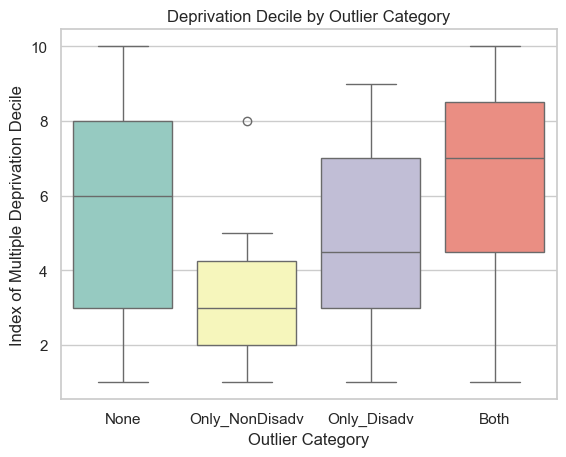
\includegraphics{P4DS_A2_Data_Analysis_Project_files/figure-pdf/cell-78-output-2.png}

\begin{Shaded}
\begin{Highlighting}[]
\CommentTok{\#  calculate descriptive statistics for outlier categories and index of multiple deprivation}

\CommentTok{\# groupby method used to group merged\_df\_2 by outlier category, then select IMDC column for further analysis}
\NormalTok{grouped }\OperatorTok{=}\NormalTok{ merged\_df\_2.groupby(}\StringTok{\textquotesingle{}Outlier\_Category\textquotesingle{}}\NormalTok{)[}\StringTok{\textquotesingle{}Index of Multiple Deprivation Decile\textquotesingle{}}\NormalTok{]}


\NormalTok{median }\OperatorTok{=}\NormalTok{ grouped.median()}
\NormalTok{q1 }\OperatorTok{=}\NormalTok{ grouped.quantile(}\FloatTok{0.25}\NormalTok{)}
\NormalTok{q3 }\OperatorTok{=}\NormalTok{ grouped.quantile(}\FloatTok{0.75}\NormalTok{)}
\NormalTok{iqr }\OperatorTok{=}\NormalTok{ q3 }\OperatorTok{{-}}\NormalTok{ q1}
\NormalTok{minimum }\OperatorTok{=}\NormalTok{ grouped.}\BuiltInTok{min}\NormalTok{()}
\NormalTok{maximum }\OperatorTok{=}\NormalTok{ grouped.}\BuiltInTok{max}\NormalTok{()}
\NormalTok{range\_ }\OperatorTok{=}\NormalTok{ maximum }\OperatorTok{{-}}\NormalTok{ minimum}


\NormalTok{summary }\OperatorTok{=}\NormalTok{ pd.DataFrame(\{}
    \StringTok{\textquotesingle{}Median\textquotesingle{}}\NormalTok{: median,}
    \StringTok{\textquotesingle{}Q1 (25\%)\textquotesingle{}}\NormalTok{: q1,}
    \StringTok{\textquotesingle{}Q3 (75\%)\textquotesingle{}}\NormalTok{: q3,}
    \StringTok{\textquotesingle{}IQR\textquotesingle{}}\NormalTok{: iqr,}
    \StringTok{\textquotesingle{}Min\textquotesingle{}}\NormalTok{: minimum,}
    \StringTok{\textquotesingle{}Max\textquotesingle{}}\NormalTok{: maximum,}
    \StringTok{\textquotesingle{}Range\textquotesingle{}}\NormalTok{: range\_}
\NormalTok{\})}

\CommentTok{\# }
\BuiltInTok{print}\NormalTok{(}\StringTok{"Summary Statistics for \textquotesingle{}Index of Multiple Deprivation Decile\textquotesingle{} by \textquotesingle{}Outlier\_Category\textquotesingle{}:"}\NormalTok{)}
\BuiltInTok{print}\NormalTok{(summary)}
\end{Highlighting}
\end{Shaded}

\begin{verbatim}
Summary Statistics for 'Index of Multiple Deprivation Decile' by 'Outlier_Category':
                  Median  Q1 (25%)  Q3 (75%)   IQR  Min   Max  Range
Outlier_Category                                                    
Both                 7.0       4.5      8.50  4.00  1.0  10.0    9.0
None                 6.0       3.0      8.00  5.00  1.0  10.0    9.0
Only_Disadv          4.5       3.0      7.00  4.00  1.0   9.0    8.0
Only_NonDisadv       3.0       2.0      4.25  2.25  1.0   8.0    7.0
\end{verbatim}

\begin{Shaded}
\begin{Highlighting}[]
\NormalTok{outlier\_performance }\OperatorTok{=}\NormalTok{ merged\_df\_2.groupby(}\StringTok{\textquotesingle{}Outlier\_Category\textquotesingle{}}\NormalTok{)[[}\StringTok{\textquotesingle{}Progress8\textquotesingle{}}\NormalTok{,}\StringTok{\textquotesingle{}Progress8\_Disadvantaged\_2022\textquotesingle{}}\NormalTok{,}\StringTok{\textquotesingle{}Progress8\_NonDisadvantaged\_2022\textquotesingle{}}\NormalTok{]].mean().reset\_index()}
\NormalTok{outlier\_performance}
\end{Highlighting}
\end{Shaded}

\begin{longtable}[]{@{}lllll@{}}
\toprule\noalign{}
& Outlier\_Category & Progress8 & Progress8\_Disadvantaged\_2022 &
Progress8\_NonDisadvantaged\_2022 \\
\midrule\noalign{}
\endhead
\bottomrule\noalign{}
\endlastfoot
0 & Both & 1.614286 & 1.417143 & 1.664286 \\
1 & None & -0.047791 & -0.486266 & 0.118369 \\
2 & Only\_Disadv & 0.946429 & 1.100000 & 0.950714 \\
3 & Only\_NonDisadv & 1.037500 & 0.626250 & 1.492500 \\
\end{longtable}

Plot box plot of progress 8 of disadvantaed pupils by outlier category

\begin{Shaded}
\begin{Highlighting}[]
\NormalTok{sns.boxplot(}
\NormalTok{    x}\OperatorTok{=}\StringTok{\textquotesingle{}Outlier\_Category\textquotesingle{}}\NormalTok{, }
\NormalTok{    y}\OperatorTok{=}\StringTok{\textquotesingle{}Progress8\_Disadvantaged\_2022\textquotesingle{}}\NormalTok{, }
\NormalTok{    data}\OperatorTok{=}\NormalTok{ merged\_df\_2,  }
\NormalTok{    palette}\OperatorTok{=}\StringTok{\textquotesingle{}Set3\textquotesingle{}}
\NormalTok{)}
\NormalTok{plt.title(}\StringTok{\textquotesingle{}Progress8 of Disadvantaged Pupils by Outlier Category\textquotesingle{}}\NormalTok{)}
\NormalTok{plt.xlabel(}\StringTok{\textquotesingle{}Outlier Category\textquotesingle{}}\NormalTok{)}
\NormalTok{plt.ylabel(}\StringTok{\textquotesingle{}Progress8 Disadvantaged 2022\textquotesingle{}}\NormalTok{)}

\NormalTok{plt.show()}


\NormalTok{sns.boxplot(}
\NormalTok{    x}\OperatorTok{=}\StringTok{\textquotesingle{}Outlier\_Category\textquotesingle{}}\NormalTok{, }
\NormalTok{    y}\OperatorTok{=}\StringTok{\textquotesingle{}Progress8\_Disadvantaged\_2022\textquotesingle{}}\NormalTok{, }
\NormalTok{    data}\OperatorTok{=}\NormalTok{ outlier\_df,  }
\NormalTok{    palette}\OperatorTok{=}\StringTok{\textquotesingle{}Set3\textquotesingle{}}
\NormalTok{)}
\NormalTok{plt.title(}\StringTok{\textquotesingle{}Progress8 of Disadvantaged Pupils by Outlier Category\textquotesingle{}}\NormalTok{)}
\NormalTok{plt.xlabel(}\StringTok{\textquotesingle{}Outlier Category\textquotesingle{}}\NormalTok{)}
\NormalTok{plt.ylabel(}\StringTok{\textquotesingle{}Progress8 Disadvantaged 2022\textquotesingle{}}\NormalTok{)}

\NormalTok{images\_dir }\OperatorTok{=} \StringTok{\textquotesingle{}images\textquotesingle{}}
\NormalTok{image\_path }\OperatorTok{=}\NormalTok{ os.path.join(images\_dir,}\StringTok{\textquotesingle{}Obj2\_Progress8 of Disadvantaged Pupils by Outlier Category.png\textquotesingle{}}\NormalTok{)}
\NormalTok{plt.savefig(image\_path)}

\NormalTok{plt.show()}
\end{Highlighting}
\end{Shaded}

\begin{verbatim}
C:\Users\saqib\AppData\Local\Temp\ipykernel_37860\3617201507.py:1: FutureWarning: 

Passing `palette` without assigning `hue` is deprecated and will be removed in v0.14.0. Assign the `x` variable to `hue` and set `legend=False` for the same effect.

  sns.boxplot(
\end{verbatim}

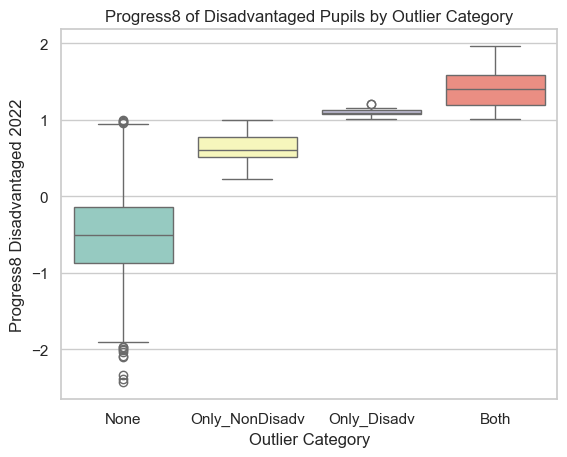
\includegraphics{P4DS_A2_Data_Analysis_Project_files/figure-pdf/cell-81-output-2.png}

\begin{verbatim}
C:\Users\saqib\AppData\Local\Temp\ipykernel_37860\3617201507.py:14: FutureWarning: 

Passing `palette` without assigning `hue` is deprecated and will be removed in v0.14.0. Assign the `x` variable to `hue` and set `legend=False` for the same effect.

  sns.boxplot(
\end{verbatim}

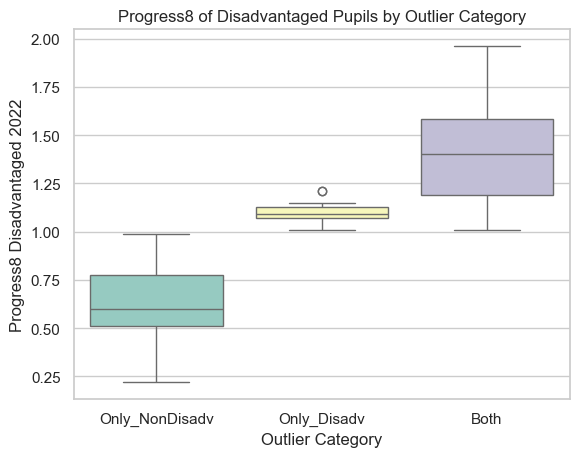
\includegraphics{P4DS_A2_Data_Analysis_Project_files/figure-pdf/cell-81-output-4.png}

\begin{Shaded}
\begin{Highlighting}[]
\CommentTok{\#calculate summary statistics for the box plot above}
\NormalTok{grouped }\OperatorTok{=}\NormalTok{ merged\_df\_2.groupby(}\StringTok{\textquotesingle{}Outlier\_Category\textquotesingle{}}\NormalTok{)[}\StringTok{\textquotesingle{}Progress8\_Disadvantaged\_2022\textquotesingle{}}\NormalTok{]}


\NormalTok{median }\OperatorTok{=}\NormalTok{ grouped.median()}
\NormalTok{q1 }\OperatorTok{=}\NormalTok{ grouped.quantile(}\FloatTok{0.25}\NormalTok{)}
\NormalTok{q3 }\OperatorTok{=}\NormalTok{ grouped.quantile(}\FloatTok{0.75}\NormalTok{)}
\NormalTok{iqr }\OperatorTok{=}\NormalTok{ q3 }\OperatorTok{{-}}\NormalTok{ q1}
\NormalTok{minimum }\OperatorTok{=}\NormalTok{ grouped.}\BuiltInTok{min}\NormalTok{()}
\NormalTok{maximum }\OperatorTok{=}\NormalTok{ grouped.}\BuiltInTok{max}\NormalTok{()}
\NormalTok{range\_ }\OperatorTok{=}\NormalTok{ maximum }\OperatorTok{{-}}\NormalTok{ minimum}


\NormalTok{summary }\OperatorTok{=}\NormalTok{ pd.DataFrame(\{}
    \StringTok{\textquotesingle{}Median\textquotesingle{}}\NormalTok{: median,}
    \StringTok{\textquotesingle{}Q1 (25\%)\textquotesingle{}}\NormalTok{: q1,}
    \StringTok{\textquotesingle{}Q3 (75\%)\textquotesingle{}}\NormalTok{: q3,}
    \StringTok{\textquotesingle{}IQR\textquotesingle{}}\NormalTok{: iqr,}
    \StringTok{\textquotesingle{}Min\textquotesingle{}}\NormalTok{: minimum,}
    \StringTok{\textquotesingle{}Max\textquotesingle{}}\NormalTok{: maximum,}
    \StringTok{\textquotesingle{}Range\textquotesingle{}}\NormalTok{: range\_}
\NormalTok{\})}

\BuiltInTok{print}\NormalTok{(}\StringTok{"Summary Statistics for \textquotesingle{}Progress8\_Disadvantaged\_2022\textquotesingle{} by \textquotesingle{}Outlier\_Category\textquotesingle{}:"}\NormalTok{)}
\BuiltInTok{print}\NormalTok{(summary)}
\end{Highlighting}
\end{Shaded}

\begin{verbatim}
Summary Statistics for 'Progress8_Disadvantaged_2022' by 'Outlier_Category':
                  Median  Q1 (25%)  Q3 (75%)    IQR   Min   Max  Range
Outlier_Category                                                      
Both                1.40      1.19     1.585  0.395  1.01  1.96   0.95
None               -0.50     -0.87    -0.140  0.730 -2.43  0.99   3.42
Only_Disadv         1.09      1.07     1.125  0.055  1.01  1.21   0.20
Only_NonDisadv      0.60      0.51     0.775  0.265  0.22  0.99   0.77
\end{verbatim}

Plot a box plot to show progress 8 scores for all outlier category types

\begin{Shaded}
\begin{Highlighting}[]
\NormalTok{sns.boxplot(}
\NormalTok{    x}\OperatorTok{=}\StringTok{\textquotesingle{}Outlier\_Category\textquotesingle{}}\NormalTok{, }
\NormalTok{    y}\OperatorTok{=}\StringTok{\textquotesingle{}Progress8\textquotesingle{}}\NormalTok{, }
\NormalTok{    data}\OperatorTok{=}\NormalTok{ merged\_df\_2,  }
\NormalTok{    palette}\OperatorTok{=}\StringTok{\textquotesingle{}Set3\textquotesingle{}}
\NormalTok{)}
\NormalTok{plt.title(}\StringTok{\textquotesingle{}Progress8  by Outlier Category\textquotesingle{}}\NormalTok{)}
\NormalTok{plt.xlabel(}\StringTok{\textquotesingle{}Outlier Category\textquotesingle{}}\NormalTok{)}
\NormalTok{plt.ylabel(}\StringTok{\textquotesingle{}Progress8 2022\textquotesingle{}}\NormalTok{)}


\NormalTok{images\_dir }\OperatorTok{=} \StringTok{\textquotesingle{}images\textquotesingle{}}
\NormalTok{image\_path }\OperatorTok{=}\NormalTok{ os.path.join(images\_dir,}\StringTok{\textquotesingle{}Obj2\_Progress8 by Outlier Category.png\textquotesingle{}}\NormalTok{)}
\NormalTok{plt.savefig(image\_path)}

\NormalTok{plt.show()}
\end{Highlighting}
\end{Shaded}

\begin{verbatim}
C:\Users\saqib\AppData\Local\Temp\ipykernel_37860\3243744368.py:1: FutureWarning: 

Passing `palette` without assigning `hue` is deprecated and will be removed in v0.14.0. Assign the `x` variable to `hue` and set `legend=False` for the same effect.

  sns.boxplot(
\end{verbatim}

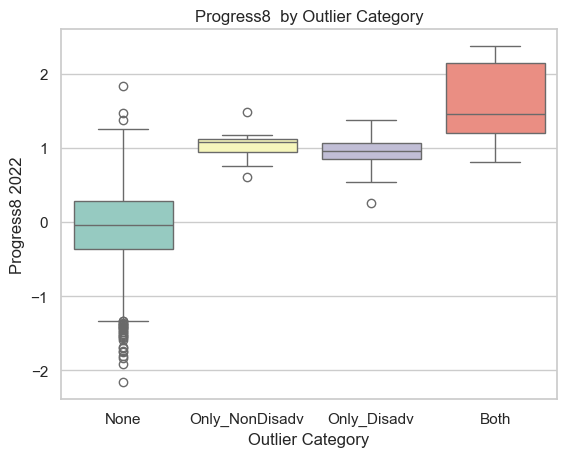
\includegraphics{P4DS_A2_Data_Analysis_Project_files/figure-pdf/cell-83-output-2.png}

\begin{Shaded}
\begin{Highlighting}[]
\CommentTok{\# Calculate summary statistics}
\NormalTok{grouped }\OperatorTok{=}\NormalTok{ merged\_df\_2.groupby(}\StringTok{\textquotesingle{}Outlier\_Category\textquotesingle{}}\NormalTok{)[}\StringTok{\textquotesingle{}Progress8\textquotesingle{}}\NormalTok{]}


\NormalTok{median }\OperatorTok{=}\NormalTok{ grouped.median()}
\NormalTok{q1 }\OperatorTok{=}\NormalTok{ grouped.quantile(}\FloatTok{0.25}\NormalTok{)}
\NormalTok{q3 }\OperatorTok{=}\NormalTok{ grouped.quantile(}\FloatTok{0.75}\NormalTok{)}
\NormalTok{iqr }\OperatorTok{=}\NormalTok{ q3 }\OperatorTok{{-}}\NormalTok{ q1}
\NormalTok{minimum }\OperatorTok{=}\NormalTok{ grouped.}\BuiltInTok{min}\NormalTok{()}
\NormalTok{maximum }\OperatorTok{=}\NormalTok{ grouped.}\BuiltInTok{max}\NormalTok{()}
\NormalTok{range\_ }\OperatorTok{=}\NormalTok{ maximum }\OperatorTok{{-}}\NormalTok{ minimum}


\NormalTok{summary }\OperatorTok{=}\NormalTok{ pd.DataFrame(\{}
    \StringTok{\textquotesingle{}Median\textquotesingle{}}\NormalTok{: median,}
    \StringTok{\textquotesingle{}Q1 (25\%)\textquotesingle{}}\NormalTok{: q1,}
    \StringTok{\textquotesingle{}Q3 (75\%)\textquotesingle{}}\NormalTok{: q3,}
    \StringTok{\textquotesingle{}IQR\textquotesingle{}}\NormalTok{: iqr,}
    \StringTok{\textquotesingle{}Min\textquotesingle{}}\NormalTok{: minimum,}
    \StringTok{\textquotesingle{}Max\textquotesingle{}}\NormalTok{: maximum,}
    \StringTok{\textquotesingle{}Range\textquotesingle{}}\NormalTok{: range\_}
\NormalTok{\})}


\BuiltInTok{print}\NormalTok{(}\StringTok{"Summary Statistics for \textquotesingle{}Progress8\textquotesingle{} by \textquotesingle{}Outlier\_Category\textquotesingle{}:"}\NormalTok{)}
\BuiltInTok{print}\NormalTok{(summary)}
\end{Highlighting}
\end{Shaded}

\begin{verbatim}
Summary Statistics for 'Progress8' by 'Outlier_Category':
                  Median  Q1 (25%)  Q3 (75%)     IQR   Min   Max  Range
Outlier_Category                                                       
Both               1.450    1.1950     2.140  0.9450  0.81  2.37   1.56
None              -0.040   -0.3600     0.290  0.6500 -2.16  1.83   3.99
Only_Disadv        0.955    0.8500     1.070  0.2200  0.25  1.38   1.13
Only_NonDisadv     1.085    0.9375     1.125  0.1875  0.61  1.49   0.88
\end{verbatim}

Using the get\_school\_details function defined earlier, I can extract
schoool details based on a URN list

\begin{Shaded}
\begin{Highlighting}[]
\NormalTok{columns }\OperatorTok{=}\NormalTok{ [}\StringTok{\textquotesingle{}School\_Name\textquotesingle{}}\NormalTok{,}
 \StringTok{\textquotesingle{}Trust\_Name\textquotesingle{}}\NormalTok{, }\StringTok{\textquotesingle{}Percent\_Disadvantaged\_2022\textquotesingle{}}\NormalTok{, }\StringTok{\textquotesingle{}Progress8\textquotesingle{}}\NormalTok{, }
 \StringTok{\textquotesingle{}Progress8\_NonDisadvantaged\_2022\textquotesingle{}}\NormalTok{, }\StringTok{\textquotesingle{}Progress8\_Disadvantaged\_2022\textquotesingle{}}\NormalTok{,}
  \StringTok{\textquotesingle{}Percent\_Not\_Disadvantaged\_2022\textquotesingle{}}\NormalTok{,}
 \StringTok{\textquotesingle{}Religious\_Character\textquotesingle{}}\NormalTok{,}
\StringTok{\textquotesingle{}Admissions\_Policy\textquotesingle{}}\NormalTok{,}
\StringTok{\textquotesingle{}School\_Gender\textquotesingle{}}\NormalTok{,}
\StringTok{\textquotesingle{}Ofsted\_Rating\textquotesingle{}}\NormalTok{,]}

\NormalTok{data\_loader }\OperatorTok{=}\NormalTok{ DataWrangler(dataframe}\OperatorTok{=}\NormalTok{outlier\_df)}
\CommentTok{\# Schools only in outliers\_disadvantaged}
\NormalTok{schools\_only\_disdv\_outliers }\OperatorTok{=}\NormalTok{ data\_loader.get\_school\_details(only\_disadvp8\_outliers, columns)}
\BuiltInTok{print}\NormalTok{(}\StringTok{"schools\_only\_disdv\_outliers:"}\NormalTok{)}
\BuiltInTok{print}\NormalTok{(schools\_only\_disdv\_outliers.to\_string(index}\OperatorTok{=}\VariableTok{False}\NormalTok{), }\StringTok{"}\CharTok{\textbackslash{}n}\StringTok{"}\NormalTok{)}

\end{Highlighting}
\end{Shaded}

\begin{verbatim}
DataWrangler initialised with the provided DataFrame.
schools_only_disdv_outliers:
                                                                        School_Name                                    Trust_Name  Percent_Disadvantaged_2022  Progress8  Progress8_NonDisadvantaged_2022  Progress8_Disadvantaged_2022  Percent_Not_Disadvantaged_2022              Religious_Character Admissions_Policy School_Gender        Ofsted_Rating
                                                        Ashcroft Technology Academy PROSPECT EDUCATION (TECHNOLOGY) TRUST LIMITED                          34       1.09                             1.17                          1.09                              66                   Does not apply     Non-selective         Mixed          Outstanding
                                                              Wren Academy Finchley                          WREN ACADEMIES TRUST                          16       1.00                             0.76                          1.02                              84                Church of England     Non-selective         Mixed          Outstanding
                                                    Lancaster Girls' Grammar School               LANCASTER GIRLS' GRAMMAR SCHOOL                           6       0.54                             0.68                          1.09                              94                              NaN         Selective         Girls                 Good
                                                                    Wilson's School                               WILSON'S SCHOOL                           5       1.33                             1.06                          1.07                              95                Church of England         Selective          Boys          Outstanding
                                                        Birmingham Ormiston Academy                   BIRMINGHAM ORMISTON ACADEMY                           8       0.25                             0.58                          1.10                              92                   Does not apply     Non-selective         Mixed                 Good
                                                           Featherstone High School               GRAND UNION MULTI ACADEMY TRUST                          31       0.84                             1.15                          1.05                              69                   Does not apply     Non-selective         Mixed          Outstanding
                                                          St Mark's Catholic School      THE DIOCESE OF WESTMINSTER ACADEMY TRUST                          10       1.30                             1.15                          1.21                              90                   Roman Catholic     Non-selective         Mixed          Outstanding
                                                            Ark Bolingbroke Academy                                   ARK SCHOOLS                          17       0.88                             0.80                          1.07                              83                              NaN     Non-selective         Mixed                 Good
                                                                Nishkam High School                          NISHKAM SCHOOL TRUST                          32       0.94                             1.11                          1.01                              68                             Sikh     Non-selective         Mixed          Outstanding
                                                       Sacred Heart Catholic School                  SACRED HEART CATHOLIC SCHOOL                          49       1.38                             1.35                          1.21                              51                   Roman Catholic     Non-selective         Mixed          Outstanding
                                                         Eden Boys' School, Preston                                STAR ACADEMIES                          21       0.97                             0.74                          1.15                              79                           Muslim     Non-selective          Boys          Outstanding
                                                         Bolton Muslim Girls School                   PROSPER MULTI ACADEMY TRUST                          19       1.01                             0.98                          1.11                              81                           Muslim     Non-selective         Girls Requires improvement
                                                  Dartford Grammar School for Girls                               THE ARETÉ TRUST                          17       0.93                             0.99                          1.09                              83                              NaN         Selective         Girls          Outstanding
St Francis Xavier School - a Joint Catholic and Church of England Voluntary Academy      NICHOLAS POSTGATE CATHOLIC ACADEMY TRUST                           8       0.79                             0.79                          1.13                              92 Roman Catholic/Church of England     Non-selective         Mixed                  NaN 
\end{verbatim}

\begin{Shaded}
\begin{Highlighting}[]
\CommentTok{\# Schools only in outliers\_not disadvantaged}
\NormalTok{data\_loader }\OperatorTok{=}\NormalTok{ DataWrangler(dataframe}\OperatorTok{=}\NormalTok{outlier\_df)}
\NormalTok{schools\_only\_nondisadv\_outliers }\OperatorTok{=}\NormalTok{ data\_loader.get\_school\_details(only\_nondisadvp8\_outliers, columns)}
\BuiltInTok{print}\NormalTok{(}\StringTok{"schools\_only\_nondisadv\_outliers:"}\NormalTok{)}
\BuiltInTok{print}\NormalTok{(schools\_only\_nondisadv\_outliers.to\_string(index}\OperatorTok{=}\VariableTok{False}\NormalTok{), }\StringTok{"}\CharTok{\textbackslash{}n}\StringTok{"}\NormalTok{)}
\end{Highlighting}
\end{Shaded}

\begin{verbatim}
DataWrangler initialised with the provided DataFrame.
schools_only_nondisadv_outliers:
                           School_Name                                                     Trust_Name  Percent_Disadvantaged_2022  Progress8  Progress8_NonDisadvantaged_2022  Progress8_Disadvantaged_2022  Percent_Not_Disadvantaged_2022 Religious_Character Admissions_Policy School_Gender Ofsted_Rating
                   Northampton Academy                                          UNITED LEARNING TRUST                          31       1.00                             1.42                          0.22                              69           Christian     Non-selective         Mixed   Outstanding
              Ark King Solomon Academy                                                    ARK SCHOOLS                          49       1.09                             1.55                          0.91                              51                 NaN     Non-selective         Mixed   Outstanding
Hillcrest School and Sixth Form Centre                         HILLCREST SCHOOL AND SIXTH FORM CENTRE                          63       0.61                             1.68                          0.42                              37      Does not apply     Non-selective         Girls          Good
              Avonbourne Girls Academy AVONBOURNE INTERNATIONAL BUSINESS AND ENTERPRISE ACADEMY TRUST                          28       0.75                             1.42                          0.54                              72                 NaN     Non-selective         Mixed          Good
                      Glenmoor Academy                                          UNITED LEARNING TRUST                          22       1.11                             1.42                          0.73                              78                 NaN     Non-selective         Girls   Outstanding
           Eden Girls' School Coventry                                                 STAR ACADEMIES                          41       1.49                             1.41                          0.99                              59              Muslim               NaN         Girls   Outstanding
               Levenshulme High School                                 EDUCATION AND LEADERSHIP TRUST                          44       1.08                             1.59                          0.61                              56      Does not apply    Not applicable         Girls   Outstanding
            Eden Girls' School, Slough                                                 STAR ACADEMIES                          31       1.17                             1.45                          0.59                              69              Muslim     Non-selective         Girls   Outstanding 
\end{verbatim}

\begin{Shaded}
\begin{Highlighting}[]

\CommentTok{\# Schools in both outliers\_disadvantaged only and outliers\_not disadvantaged}

\NormalTok{data\_loader }\OperatorTok{=}\NormalTok{ DataWrangler(dataframe}\OperatorTok{=}\NormalTok{outlier\_df)}

\NormalTok{schools\_both }\OperatorTok{=}\NormalTok{ data\_loader.get\_school\_details(both\_p8\_outliers, columns)}
\BuiltInTok{print}\NormalTok{(}\StringTok{"Schools in both disadv and nondisadv outliers:"}\NormalTok{)}
\BuiltInTok{print}\NormalTok{(schools\_both.to\_string(index}\OperatorTok{=}\VariableTok{False}\NormalTok{))}
\end{Highlighting}
\end{Shaded}

\begin{verbatim}
DataWrangler initialised with the provided DataFrame.
Schools in both disadv and nondisadv outliers:
                                School_Name                                Trust_Name  Percent_Disadvantaged_2022  Progress8  Progress8_NonDisadvantaged_2022  Progress8_Disadvantaged_2022  Percent_Not_Disadvantaged_2022 Religious_Character Admissions_Policy School_Gender Ofsted_Rating
                   Bentley Wood High School                    THE BENTLEY WOOD TRUST                          28       1.05                             1.48                          1.01                              72      Does not apply     Non-selective         Girls   Outstanding
                  Michaela Community School          MICHAELA COMMUNITY SCHOOLS TRUST                          26       2.37                             2.37                          1.96                              74                 NaN     Non-selective         Mixed   Outstanding
         Tauheedul Islam Girls' High School                            STAR ACADEMIES                          17       2.30                             1.76                          1.56                              83              Muslim     Non-selective         Girls   Outstanding
                     The Hurlingham Academy                     UNITED LEARNING TRUST                          38       0.81                             1.42                          1.19                              62      Does not apply     Non-selective         Mixed   Outstanding
                  Ealing Fields High School TWYFORD CHURCH OF ENGLAND ACADEMIES TRUST                          37       1.34                             1.41                          1.19                              63                 NaN               NaN         Mixed          Good
Eden Girls'  Leadership Academy, Birmingham                            STAR ACADEMIES                          45       1.98                             1.84                          1.40                              55              Muslim     Non-selective         Girls   Outstanding
                 St Peter's Catholic School           XAVIER CATHOLIC EDUCATION TRUST                           5       1.45                             1.37                          1.61                              95      Roman Catholic     Non-selective         Mixed   Outstanding
\end{verbatim}

I will also evaluate the categorical columns in the outlier schools

\begin{Shaded}
\begin{Highlighting}[]
\NormalTok{categorical\_columns}\OperatorTok{=}\NormalTok{ outlier\_df[[}\StringTok{\textquotesingle{}School\_Type\textquotesingle{}}\NormalTok{,}\StringTok{\textquotesingle{}School\_College\_Type\textquotesingle{}}\NormalTok{,}
\StringTok{\textquotesingle{}Religious\_Character\textquotesingle{}}\NormalTok{,}
\StringTok{\textquotesingle{}Admissions\_Policy\textquotesingle{}}\NormalTok{,}
 \StringTok{\textquotesingle{}School\_Gender\textquotesingle{}}\NormalTok{,}
\StringTok{\textquotesingle{}Ofsted\_Rating\textquotesingle{}}\NormalTok{,}\StringTok{\textquotesingle{}Trust\_Name\textquotesingle{}}\NormalTok{,}\StringTok{\textquotesingle{}Outlier\_Category\textquotesingle{}}\NormalTok{]]}
                                             
\end{Highlighting}
\end{Shaded}

\begin{Shaded}
\begin{Highlighting}[]
\NormalTok{numerical\_variables }\OperatorTok{=}\NormalTok{ outlier\_df[[}\StringTok{\textquotesingle{}FSM\_Funding\textquotesingle{}}\NormalTok{,}
                                                \StringTok{\textquotesingle{}Pupil\_Premium\_Funding\textquotesingle{}}\NormalTok{,}
                                                 \StringTok{\textquotesingle{}Pupil\_Premium\_Pupils\textquotesingle{}}\NormalTok{,}
                                          \StringTok{\textquotesingle{}School\_Led\_Tutoring\_Funding\textquotesingle{}}\NormalTok{,}
                                                        \StringTok{\textquotesingle{}Total\_Funding\textquotesingle{}}\NormalTok{,}\StringTok{\textquotesingle{}Attainment8\textquotesingle{}}\NormalTok{,}
                                                            \StringTok{\textquotesingle{}Progress8\textquotesingle{}}\NormalTok{,}
                                           \StringTok{\textquotesingle{}Percent\_Disadvantaged\_2022\textquotesingle{}}\NormalTok{,}
                                       \StringTok{\textquotesingle{}Percent\_Not\_Disadvantaged\_2022\textquotesingle{}}\NormalTok{,}
                                  \StringTok{\textquotesingle{}Percent\_Disadvantaged\_Strong\_Passes\textquotesingle{}}\NormalTok{,}
                              \StringTok{\textquotesingle{}Percent\_Not\_Disadvantaged\_Strong\_Passes\textquotesingle{}}\NormalTok{,}
       \StringTok{\textquotesingle{}Average Attainment 8 score per non{-}disadvantaged pupil  {-} 2022\textquotesingle{}}\NormalTok{,}
                                      \StringTok{\textquotesingle{}Progress8\_NonDisadvantaged\_2022\textquotesingle{}}\NormalTok{,}
                                   \StringTok{\textquotesingle{}Attainment8\_Disadvantaged\_2022\textquotesingle{}}\NormalTok{,}
                                         \StringTok{\textquotesingle{}Progress8\_Disadvantaged\_2022\textquotesingle{}}\NormalTok{,}
                                        \StringTok{\textquotesingle{}Progress8\_Maths\_Disadvantaged\textquotesingle{}}\NormalTok{,}
                                      \StringTok{\textquotesingle{}Progress8\_English\_Disadvantaged\textquotesingle{}}\NormalTok{,}
                                     \StringTok{\textquotesingle{}Progress8\_Maths\_NonDisadvantaged\textquotesingle{}}\NormalTok{,}
                                   \StringTok{\textquotesingle{}Progress8\_English\_NonDisadvantaged\textquotesingle{}}\NormalTok{, }\StringTok{\textquotesingle{}Index of Multiple Deprivation Decile\textquotesingle{}}\NormalTok{]]}
\end{Highlighting}
\end{Shaded}

\begin{Shaded}
\begin{Highlighting}[]
\NormalTok{numerical\_variables.describe()}
\end{Highlighting}
\end{Shaded}

\begin{longtable}[]{@{}lllllllllllllllllllll@{}}
\toprule\noalign{}
& FSM\_Funding & Pupil\_Premium\_Funding & Pupil\_Premium\_Pupils &
School\_Led\_Tutoring\_Funding & Total\_Funding & Attainment8 &
Progress8 & Percent\_Disadvantaged\_2022 &
Percent\_Not\_Disadvantaged\_2022 &
Percent\_Disadvantaged\_Strong\_Passes &
Percent\_Not\_Disadvantaged\_Strong\_Passes & Average Attainment 8 score
per non-disadvantaged pupil - 2022 & Progress8\_NonDisadvantaged\_2022 &
Attainment8\_Disadvantaged\_2022 & Progress8\_Disadvantaged\_2022 &
Progress8\_Maths\_Disadvantaged & Progress8\_English\_Disadvantaged &
Progress8\_Maths\_NonDisadvantaged &
Progress8\_English\_NonDisadvantaged & Index of Multiple Deprivation
Decile \\
\midrule\noalign{}
\endhead
\bottomrule\noalign{}
\endlastfoot
count & 29.000000 & 29.000000 & 29.000000 & 29.000000 & 2.900000e+01 &
29.000000 & 29.000000 & 29.000000 & 29.000000 & 29.000000 & 29.000000 &
29.000000 & 29.000000 & 29.000000 & 29.000000 & 29.000000 & 29.000000 &
29.000000 & 29.000000 & 29.000000 \\
mean & 105475.413793 & 221438.344828 & 219.586207 & 36555.517241 &
5.670275e+06 & 61.465517 & 1.132759 & 26.827586 & 73.172414 & 63.689655
& 76.689655 & 65.731034 & 1.272414 & 59.410345 & 1.045862 & 0.749655 &
0.995172 & 1.103103 & 1.256207 & 4.896552 \\
std & 138064.982769 & 143085.321561 & 131.774027 & 21375.221128 &
2.015004e+06 & 8.462956 & 0.466835 & 15.099832 & 15.099832 & 17.730328 &
12.742234 & 7.008368 & 0.397911 & 8.321502 & 0.354718 & 0.664543 &
0.570705 & 0.578225 & 0.461793 & 2.730055 \\
min & 0.000000 & 39400.000000 & 40.000000 & 6480.000000 & 2.223628e+06 &
50.500000 & 0.250000 & 5.000000 & 37.000000 & 29.000000 & 56.000000 &
54.100000 & 0.580000 & 45.700000 & 0.220000 & -0.680000 & -0.280000 &
0.020000 & 0.610000 & 1.000000 \\
25\% & 37515.000000 & 129035.000000 & 131.000000 & 22194.000000 &
4.234625e+06 & 56.200000 & 0.880000 & 17.000000 & 63.000000 & 53.000000
& 65.000000 & 62.900000 & 0.990000 & 55.000000 & 0.990000 & 0.360000 &
0.660000 & 0.720000 & 0.970000 & 3.000000 \\
50\% & 74260.000000 & 183210.000000 & 186.000000 & 31590.000000 &
5.358210e+06 & 59.900000 & 1.050000 & 28.000000 & 72.000000 & 62.000000
& 77.000000 & 65.300000 & 1.370000 & 57.800000 & 1.090000 & 0.830000 &
0.890000 & 1.050000 & 1.150000 & 4.000000 \\
75\% & 121260.000000 & 279740.000000 & 284.000000 & 46818.000000 &
6.200771e+06 & 64.900000 & 1.330000 & 37.000000 & 83.000000 & 71.000000
& 84.000000 & 67.300000 & 1.450000 & 62.100000 & 1.190000 & 0.970000 &
1.270000 & 1.400000 & 1.480000 & 7.000000 \\
max & 730864.000000 & 681170.000000 & 562.000000 & 86994.000000 &
1.047014e+07 & 86.400000 & 2.370000 & 63.000000 & 95.000000 & 100.000000
& 100.000000 & 85.500000 & 2.370000 & 84.100000 & 1.960000 & 2.480000 &
2.190000 & 2.950000 & 2.330000 & 10.000000 \\
\end{longtable}

\begin{Shaded}
\begin{Highlighting}[]

\CommentTok{\#Standardise the numerical values to ensure accurate corrlation}

\NormalTok{scaler }\OperatorTok{=}\NormalTok{ StandardScaler() }\CommentTok{\# use standard scaler which will make each feature have 0 mean and SD=1}

\NormalTok{scaled\_data }\OperatorTok{=}\NormalTok{ scaler.fit\_transform(numerical\_variables)}


\NormalTok{scaled\_numerical\_df }\OperatorTok{=}\NormalTok{ pd.DataFrame(scaled\_data, columns}\OperatorTok{=}\NormalTok{numerical\_variables.columns)}


\NormalTok{merged\_df\_2[scaled\_numerical\_df.columns] }\OperatorTok{=}\NormalTok{ scaled\_numerical\_df}


\NormalTok{scaled\_numerical\_df.head()}
\end{Highlighting}
\end{Shaded}

\begin{longtable}[]{@{}lllllllllllllllllllll@{}}
\toprule\noalign{}
& FSM\_Funding & Pupil\_Premium\_Funding & Pupil\_Premium\_Pupils &
School\_Led\_Tutoring\_Funding & Total\_Funding & Attainment8 &
Progress8 & Percent\_Disadvantaged\_2022 &
Percent\_Not\_Disadvantaged\_2022 &
Percent\_Disadvantaged\_Strong\_Passes &
Percent\_Not\_Disadvantaged\_Strong\_Passes & Average Attainment 8 score
per non-disadvantaged pupil - 2022 & Progress8\_NonDisadvantaged\_2022 &
Attainment8\_Disadvantaged\_2022 & Progress8\_Disadvantaged\_2022 &
Progress8\_Maths\_Disadvantaged & Progress8\_English\_Disadvantaged &
Progress8\_Maths\_NonDisadvantaged &
Progress8\_English\_NonDisadvantaged & Index of Multiple Deprivation
Decile \\
\midrule\noalign{}
\endhead
\bottomrule\noalign{}
\endlastfoot
0 & 0.341747 & 1.458545 & 1.648210 & 1.768970 & 2.044712 & -1.005983 &
-0.289414 & 0.281213 & -0.281213 & -1.072765 & -0.933633 & -0.977428 &
0.377468 & -1.676744 & -2.369430 & 0.092414 & -0.330206 & -0.163866 &
-0.564629 & -1.079766 \\
1 & 0.199734 & 3.269861 & 2.644487 & 2.401438 & 1.378092 & -0.392690 &
-0.093214 & 1.494379 & -1.494379 & -0.326580 & 0.184523 & -0.178761 &
0.709957 & -0.258090 & -0.389793 & 0.245557 & 0.490082 & 0.205743 &
0.911918 & -1.079766 \\
2 & 4.609846 & 0.901583 & 1.038088 & 1.136931 & 1.618857 & 0.220603 &
-0.093214 & 0.483407 & -0.483407 & 0.304808 & 0.583865 & 0.184269 &
-0.261934 & -0.025725 & 0.126633 & 0.414014 & -0.098385 & 0.575352 &
-1.093541 & 0.784116 \\
3 & -0.213244 & 0.050084 & -0.089481 & -0.105293 & 1.051198 & 0.220603 &
-0.289414 & -0.729759 & 0.729759 & 0.419605 & 0.503996 & 0.082621 &
-1.310553 & 0.328939 & -0.074199 & -0.336386 & -0.740349 & 0.205743 &
-0.718895 & 0.784116 \\
4 & -0.652757 & -1.273738 & -1.363788 & -1.401080 & -0.725091 & 1.218708
& -1.292214 & -1.403740 & 1.403740 & 1.108392 & 1.462416 & 1.679955 &
-1.515162 & 1.808741 & 0.126633 & -1.699358 & -2.273930 & -1.431098 &
-1.424112 & 0.038563 \\
\end{longtable}

As part of the analysis, I will create a heatmap of numerical variables

\begin{Shaded}
\begin{Highlighting}[]

\CommentTok{\# Correlation matrix}
\NormalTok{corr\_matrix }\OperatorTok{=}\NormalTok{ numerical\_variables.corr()}
\NormalTok{plt.figure(figsize}\OperatorTok{=}\NormalTok{(}\DecValTok{18}\NormalTok{,}\DecValTok{18}\NormalTok{))}

\NormalTok{images\_dir }\OperatorTok{=} \StringTok{\textquotesingle{}images\textquotesingle{}}
\NormalTok{image\_path }\OperatorTok{=}\NormalTok{ os.path.join(images\_dir,}\StringTok{\textquotesingle{}Obj2\_Heatmap Outlier Schools.png\textquotesingle{}}\NormalTok{)}
\NormalTok{plt.savefig(image\_path)}


\CommentTok{\# Heatmap}
\NormalTok{sns.heatmap(corr\_matrix, annot}\OperatorTok{=}\VariableTok{True}\NormalTok{)}
\NormalTok{plt.show()}
\end{Highlighting}
\end{Shaded}

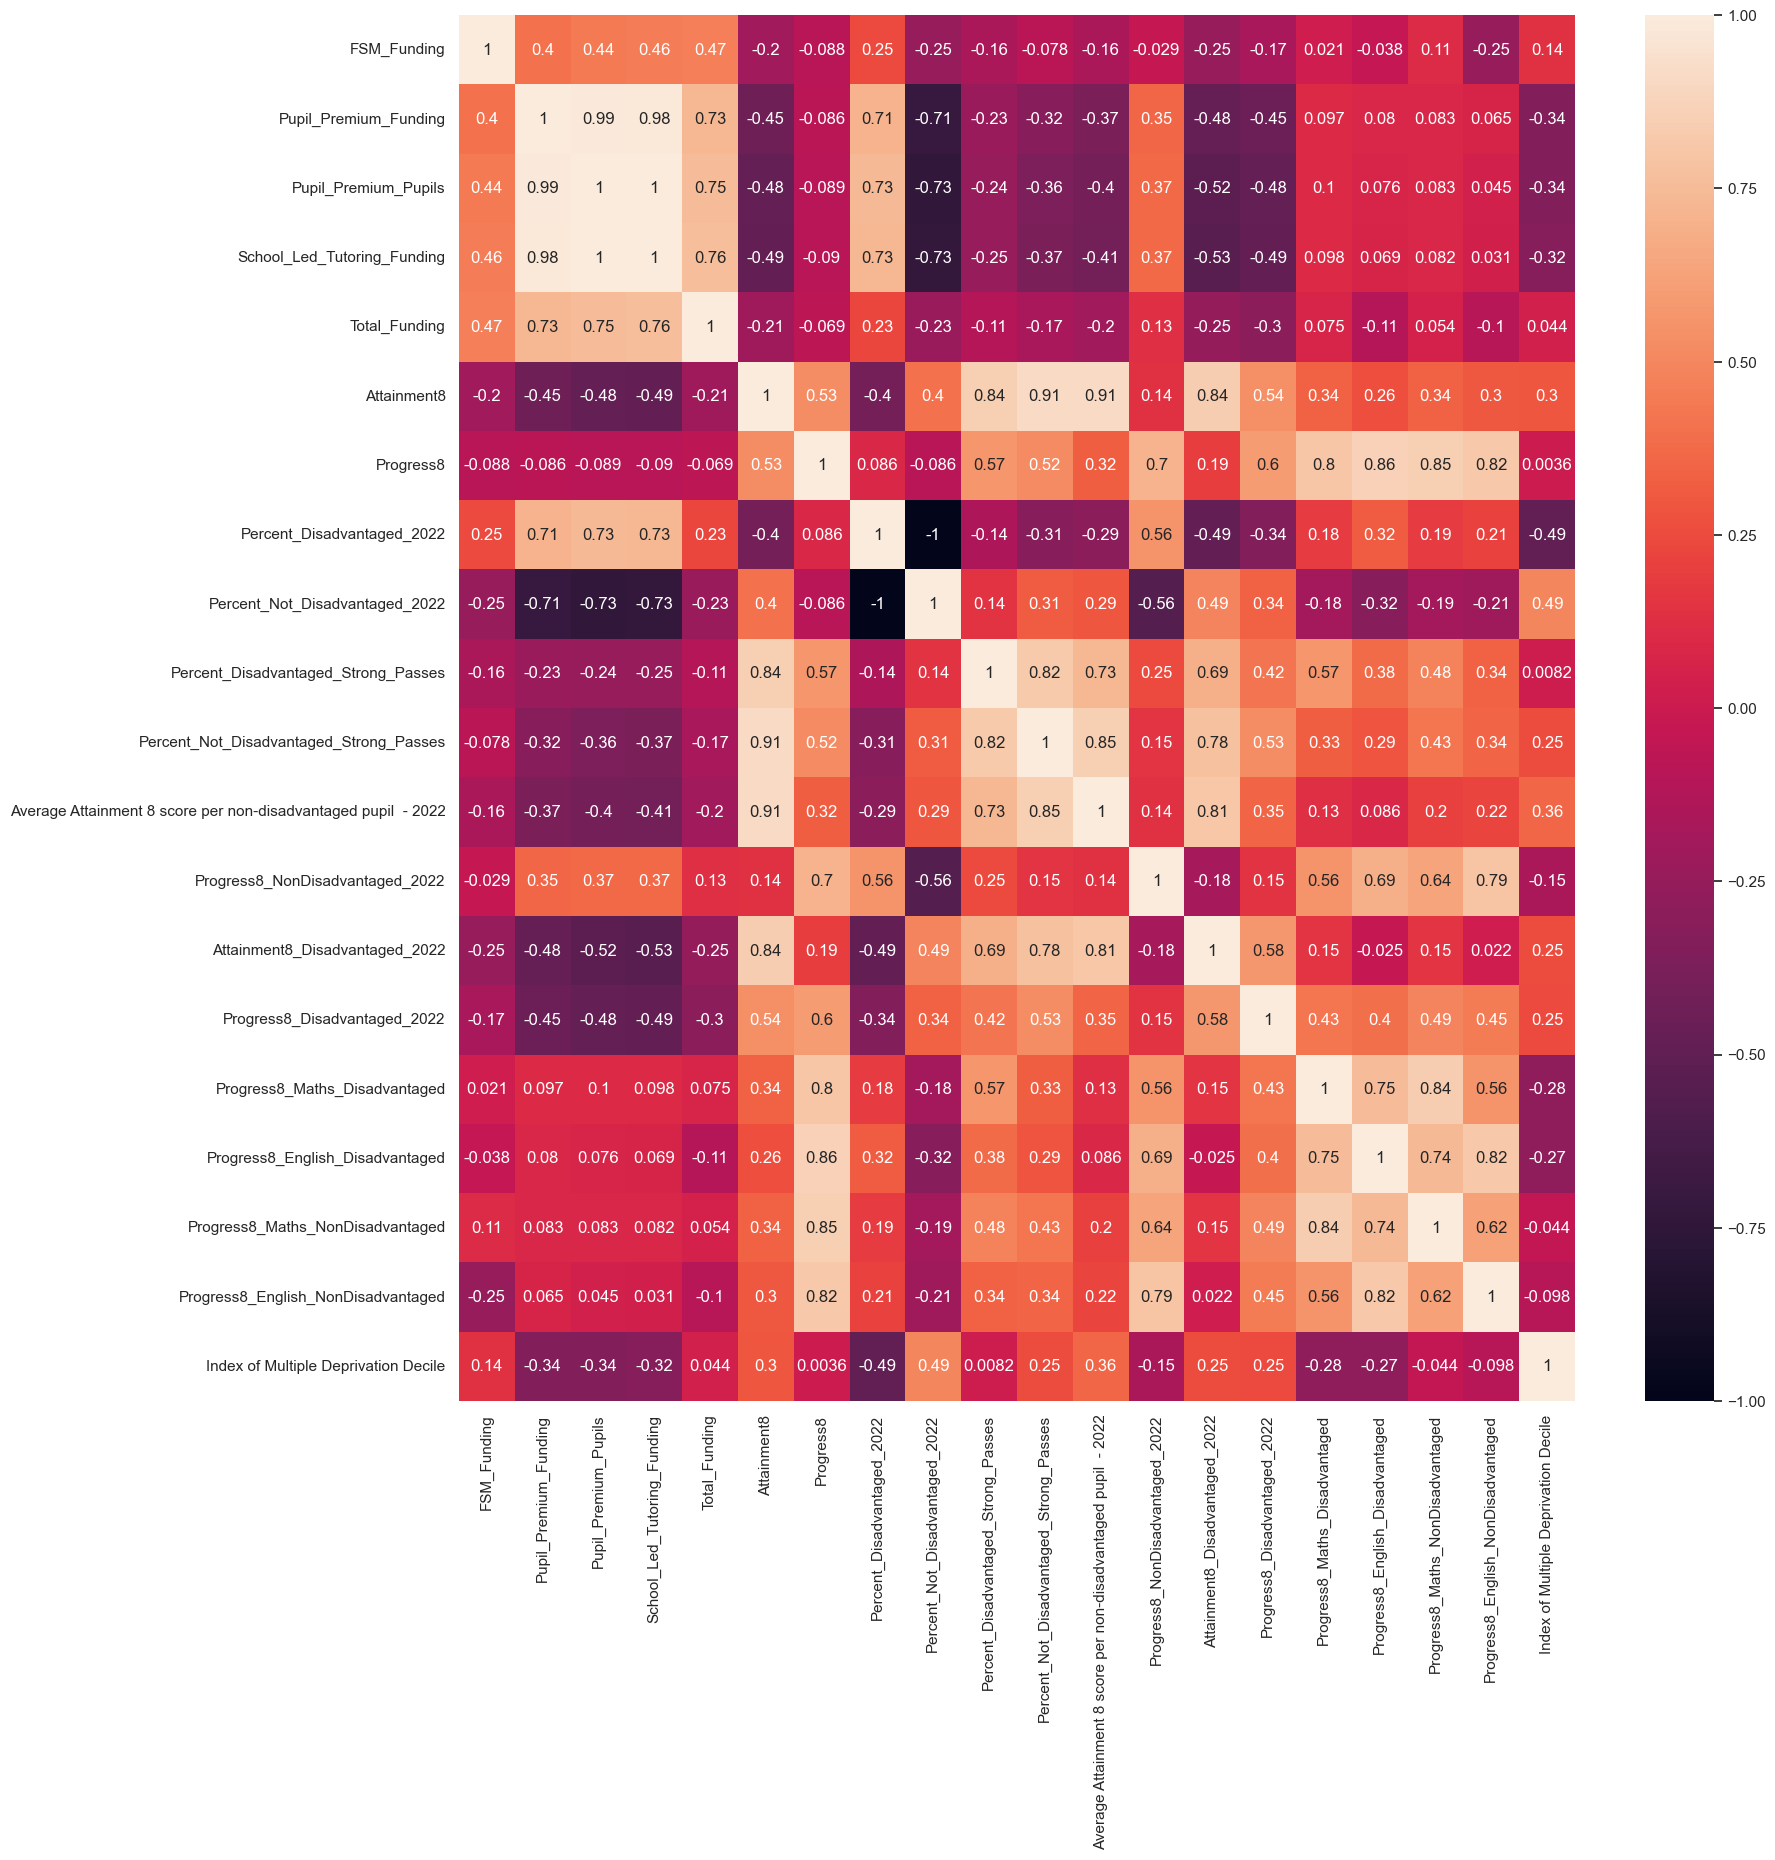
\includegraphics{P4DS_A2_Data_Analysis_Project_files/figure-pdf/cell-93-output-1.png}

\paragraph{Objective 3 Code: Identify and evaluate the top performing
multi-academy trusts in supporting disadvantaged
pupils}\label{objective-3-code-identify-and-evaluate-the-top-performing-multi-academy-trusts-in-supporting-disadvantaged-pupils}

\begin{Shaded}
\begin{Highlighting}[]
\NormalTok{merged\_df\_3}\OperatorTok{=}\NormalTok{merged\_df.copy() }\CommentTok{\# make another copy of merged\_df}
\end{Highlighting}
\end{Shaded}

\begin{Shaded}
\begin{Highlighting}[]
\CommentTok{\# group schools by MAT for analysis}
\NormalTok{MAT\_performance }\OperatorTok{=}\NormalTok{ merged\_df\_3.groupby(}\StringTok{\textquotesingle{}Trust\_Name\textquotesingle{}}\NormalTok{)[[}\StringTok{\textquotesingle{}Progress8\textquotesingle{}}\NormalTok{,}\StringTok{\textquotesingle{}Progress8\_Disadvantaged\_2022\textquotesingle{}}\NormalTok{,}\StringTok{\textquotesingle{}progress8\_gap\textquotesingle{}}\NormalTok{,}
                                                      \StringTok{\textquotesingle{}attainment8\_gap\textquotesingle{}}\NormalTok{,}
                                                            \StringTok{\textquotesingle{}maths\_gap\textquotesingle{}}\NormalTok{,}
                                                          \StringTok{\textquotesingle{}english\_gap\textquotesingle{}}\NormalTok{,}
                                                           \StringTok{\textquotesingle{}5\_GCSE\_gap\textquotesingle{}}\NormalTok{,}
                                               \StringTok{\textquotesingle{}pupilpremium\_per\_pupil\textquotesingle{}}\NormalTok{,}\StringTok{\textquotesingle{}Progress8\_NonDisadvantaged\_2022\textquotesingle{}}\NormalTok{,}\StringTok{\textquotesingle{}Index of Multiple Deprivation Decile\textquotesingle{}}\NormalTok{]].mean().reset\_index()}
\NormalTok{MAT\_performance.head()}
\end{Highlighting}
\end{Shaded}

\begin{longtable}[]{@{}llllllllllll@{}}
\toprule\noalign{}
& Trust\_Name & Progress8 & Progress8\_Disadvantaged\_2022 &
progress8\_gap & attainment8\_gap & maths\_gap & english\_gap &
5\_GCSE\_gap & pupilpremium\_per\_pupil &
Progress8\_NonDisadvantaged\_2022 & Index of Multiple Deprivation
Decile \\
\midrule\noalign{}
\endhead
\bottomrule\noalign{}
\endlastfoot
0 & 5 DIMENSIONS TRUST & -0.13 & -0.89 & 0.930 & 14.40 & 0.43 & 0.93 &
18.0 & 983.164179 & 0.040 & 6.0 \\
1 & ABBEY ACADEMIES TRUST & -0.43 & -1.11 & 0.930 & 10.50 & 0.59 & 0.48
& 26.0 & 985.000000 & -0.180 & 7.0 \\
2 & ABBEY COLLEGE, RAMSEY & -0.10 & -0.55 & 0.690 & 14.60 & 0.25 & 0.26
& 14.0 & 985.000000 & 0.140 & 6.0 \\
3 & ABBEY MULTI ACADEMY TRUST & 0.07 & -0.05 & 0.305 & 7.75 & 0.41 &
0.44 & 17.0 & 984.078652 & 0.255 & 1.0 \\
4 & ABBS CROSS ACADEMY AND ARTS COLLEGE & 0.04 & -1.17 & 0.990 & 16.00 &
0.35 & 0.31 & 17.0 & 985.000000 & -0.180 & 8.0 \\
\end{longtable}

\begin{Shaded}
\begin{Highlighting}[]
\NormalTok{MAT\_performance\_sorted }\OperatorTok{=}\NormalTok{ MAT\_performance.sort\_values(by}\OperatorTok{=}\StringTok{\textquotesingle{}Progress8\_Disadvantaged\_2022\textquotesingle{}}\NormalTok{, ascending}\OperatorTok{=}\VariableTok{False}\NormalTok{)}
\CommentTok{\#we can now sort by progress 8 score of disadvantaged pupils}
\NormalTok{MAT\_performance\_sorted.head()}

\end{Highlighting}
\end{Shaded}

\begin{longtable}[]{@{}llllllllllll@{}}
\toprule\noalign{}
& Trust\_Name & Progress8 & Progress8\_Disadvantaged\_2022 &
progress8\_gap & attainment8\_gap & maths\_gap & english\_gap &
5\_GCSE\_gap & pupilpremium\_per\_pupil &
Progress8\_NonDisadvantaged\_2022 & Index of Multiple Deprivation
Decile \\
\midrule\noalign{}
\endhead
\bottomrule\noalign{}
\endlastfoot
654 & MICHAELA COMMUNITY SCHOOLS TRUST & 2.37 & 1.96 & 0.41 & 6.3 & 0.47
& 0.25 & 5.0 & 985.0 & 2.37 & 5.0 \\
833 & SACRED HEART CATHOLIC SCHOOL & 1.38 & 1.21 & 0.14 & 3.2 & 0.49 &
0.15 & 15.0 & 985.0 & 1.35 & 4.0 \\
780 & PROSPER MULTI ACADEMY TRUST & 1.01 & 1.11 & -0.13 & 7.6 & -0.36 &
0.59 & 15.0 & 985.0 & 0.98 & 3.0 \\
111 & BIRMINGHAM ORMISTON ACADEMY & 0.25 & 1.10 & -0.52 & -2.9 & 0.70 &
0.12 & 36.0 & 985.0 & 0.58 & 4.0 \\
587 & LANCASTER GIRLS\textquotesingle{} GRAMMAR SCHOOL & 0.54 & 1.09 &
-0.41 & 3.1 & 0.65 & 0.89 & 12.0 & 985.0 & 0.68 & 5.0 \\
\end{longtable}

\begin{Shaded}
\begin{Highlighting}[]
\CommentTok{\# Group by Trust and calculate mean scores along with the count of schools}
\NormalTok{MAT\_performance }\OperatorTok{=}\NormalTok{ merged\_df\_3.groupby(}\StringTok{\textquotesingle{}Trust\_Name\textquotesingle{}}\NormalTok{).agg(}
\NormalTok{    avg\_progress8\_score}\OperatorTok{=}\NormalTok{(}\StringTok{\textquotesingle{}Progress8\textquotesingle{}}\NormalTok{, }\StringTok{\textquotesingle{}mean\textquotesingle{}}\NormalTok{),}
\NormalTok{    prog8\_score\_disadv}\OperatorTok{=}\NormalTok{(}\StringTok{\textquotesingle{}Progress8\_Disadvantaged\_2022\textquotesingle{}}\NormalTok{, }\StringTok{\textquotesingle{}mean\textquotesingle{}}\NormalTok{),}
\NormalTok{    prog8\_score\_nondisadv}\OperatorTok{=}\NormalTok{(}\StringTok{\textquotesingle{}Progress8\_NonDisadvantaged\_2022\textquotesingle{}}\NormalTok{, }\StringTok{\textquotesingle{}mean\textquotesingle{}}\NormalTok{),}
\NormalTok{    progress8\_gap}\OperatorTok{=}\NormalTok{(}\StringTok{\textquotesingle{}progress8\_gap\textquotesingle{}}\NormalTok{, }\StringTok{\textquotesingle{}mean\textquotesingle{}}\NormalTok{),}
\NormalTok{    attainment8\_gap}\OperatorTok{=}\NormalTok{(}\StringTok{\textquotesingle{}attainment8\_gap\textquotesingle{}}\NormalTok{, }\StringTok{\textquotesingle{}mean\textquotesingle{}}\NormalTok{),}
\NormalTok{    maths\_gap}\OperatorTok{=}\NormalTok{(}\StringTok{\textquotesingle{}maths\_gap\textquotesingle{}}\NormalTok{, }\StringTok{\textquotesingle{}mean\textquotesingle{}}\NormalTok{),}
\NormalTok{    english\_gap}\OperatorTok{=}\NormalTok{(}\StringTok{\textquotesingle{}english\_gap\textquotesingle{}}\NormalTok{, }\StringTok{\textquotesingle{}mean\textquotesingle{}}\NormalTok{),}
\NormalTok{    FiveGCSE\_gap}\OperatorTok{=}\NormalTok{(}\StringTok{\textquotesingle{}5\_GCSE\_gap\textquotesingle{}}\NormalTok{, }\StringTok{\textquotesingle{}mean\textquotesingle{}}\NormalTok{),}
\NormalTok{ deprivation\_index}\OperatorTok{=}\NormalTok{ (}\StringTok{\textquotesingle{}Index of Multiple Deprivation Decile\textquotesingle{}}\NormalTok{,}\StringTok{\textquotesingle{}mean\textquotesingle{}}\NormalTok{),}
\NormalTok{    school\_count}\OperatorTok{=}\NormalTok{(}\StringTok{\textquotesingle{}URN\textquotesingle{}}\NormalTok{, }\StringTok{\textquotesingle{}count\textquotesingle{}}\NormalTok{)  }\CommentTok{\# Counting the number of schools per Group Name}
\NormalTok{).reset\_index()}

\CommentTok{\# Sort the MAT\_performance DataFrame by \textquotesingle{}avg\_progress8\_score\textquotesingle{} in descending order}
\NormalTok{MAT\_performance\_sorted }\OperatorTok{=}\NormalTok{ MAT\_performance.sort\_values(by}\OperatorTok{=}\StringTok{\textquotesingle{}prog8\_score\_disadv\textquotesingle{}}\NormalTok{, ascending}\OperatorTok{=}\VariableTok{False}\NormalTok{)}

\NormalTok{MAT\_performance\_sorted.head()}
\end{Highlighting}
\end{Shaded}

\begin{longtable}[]{@{}llllllllllll@{}}
\toprule\noalign{}
& Trust\_Name & avg\_progress8\_score & prog8\_score\_disadv &
prog8\_score\_nondisadv & progress8\_gap & attainment8\_gap & maths\_gap
& english\_gap & FiveGCSE\_gap & deprivation\_index & school\_count \\
\midrule\noalign{}
\endhead
\bottomrule\noalign{}
\endlastfoot
654 & MICHAELA COMMUNITY SCHOOLS TRUST & 2.37 & 1.96 & 2.37 & 0.41 & 6.3
& 0.47 & 0.25 & 5.0 & 5.0 & 1 \\
833 & SACRED HEART CATHOLIC SCHOOL & 1.38 & 1.21 & 1.35 & 0.14 & 3.2 &
0.49 & 0.15 & 15.0 & 4.0 & 1 \\
780 & PROSPER MULTI ACADEMY TRUST & 1.01 & 1.11 & 0.98 & -0.13 & 7.6 &
-0.36 & 0.59 & 15.0 & 3.0 & 1 \\
111 & BIRMINGHAM ORMISTON ACADEMY & 0.25 & 1.10 & 0.58 & -0.52 & -2.9 &
0.70 & 0.12 & 36.0 & 4.0 & 1 \\
587 & LANCASTER GIRLS\textquotesingle{} GRAMMAR SCHOOL & 0.54 & 1.09 &
0.68 & -0.41 & 3.1 & 0.65 & 0.89 & 12.0 & 5.0 & 1 \\
\end{longtable}

A number of MATs have 1 or 2 schools, so I will filter for those with at
least 4 schools as I want to explore organisational impact of Trusts
working with mutiple schools

\begin{Shaded}
\begin{Highlighting}[]

\CommentTok{\# Filter MATs with school\_count \textgreater{}= 4 }
\NormalTok{MAT\_performance\_filtered }\OperatorTok{=}\NormalTok{ MAT\_performance[MAT\_performance[}\StringTok{\textquotesingle{}school\_count\textquotesingle{}}\NormalTok{] }\OperatorTok{\textgreater{}=} \DecValTok{4}\NormalTok{]}

\CommentTok{\# top 10 MATs with the highest average Progress 8 scores disadvantaged and at least 4 schools}
\NormalTok{MAT\_performance\_sorted }\OperatorTok{=}\NormalTok{ MAT\_performance\_filtered.sort\_values(by}\OperatorTok{=}\StringTok{\textquotesingle{}prog8\_score\_disadv\textquotesingle{}}\NormalTok{, ascending}\OperatorTok{=}\VariableTok{False}\NormalTok{)}


\NormalTok{Top\_10MAT }\OperatorTok{=}\NormalTok{ MAT\_performance\_sorted.head(}\DecValTok{10}\NormalTok{)}
\BuiltInTok{print}\NormalTok{(Top\_10MAT)}
\end{Highlighting}
\end{Shaded}

\begin{verbatim}
                                    Trust_Name  avg_progress8_score  \
975                             STAR ACADEMIES             0.640526   
219                    CHILTERN LEARNING TRUST             0.424000   
57                                 ARK SCHOOLS             0.208421   
1096  THE DIOCESE OF WESTMINSTER ACADEMY TRUST             0.645000   
628               LOXFORD SCHOOL TRUST LIMITED             0.337500   
335             EDUCATION AND LEADERSHIP TRUST             0.260000   
1123                 THE GORSE ACADEMIES TRUST             0.435714   
451                          HARRIS FEDERATION             0.265652   
827                    RUSSELL EDUCATION TRUST             0.466000   
1323                     UNITED LEARNING TRUST             0.146757   

      prog8_score_disadv  prog8_score_nondisadv  progress8_gap  \
975             0.231579               0.495789       0.264211   
219             0.226000               0.634000       0.408000   
57              0.085789               0.435789       0.350000   
1096            0.076667               0.691667       0.615000   
628             0.075000               0.422500       0.347500   
335             0.030000               0.762500       0.732500   
1123            0.024286               0.645714       0.621429   
451             0.020870               0.644348       0.623478   
827            -0.068000               0.534000       0.602000   
1323           -0.098378               0.487297       0.585676   

      attainment8_gap  maths_gap  english_gap  FiveGCSE_gap  \
975          6.247368   0.294737     0.244211     10.210526   
219          7.680000   0.456000     0.348000     17.000000   
57           6.131579   0.437368     0.290526     16.263158   
1096        10.700000   0.303333     0.161667     20.833333   
628          5.075000   0.312500     0.147500     15.250000   
335         10.450000   0.575000     0.527500     18.500000   
1123        12.842857   0.675714     0.810000     25.571429   
451         10.065217   0.574783     0.400435     19.826087   
827         15.380000   0.730000     0.836000     34.000000   
1323         9.802703   0.518108     0.507027     18.297297   

      deprivation_index  school_count  
975            2.421053            19  
219            4.600000             5  
57             3.157895            19  
1096           5.833333             6  
628            5.000000             4  
335            3.000000             4  
1123           5.714286             7  
451            4.956522            23  
827            5.200000             5  
1323           4.297297            37  
\end{verbatim}

\begin{Shaded}
\begin{Highlighting}[]
\CommentTok{\#represent data on a graphs}

\CommentTok{\# Set the style }
\NormalTok{sns.}\BuiltInTok{set}\NormalTok{(style}\OperatorTok{=}\StringTok{"whitegrid"}\NormalTok{)}

\CommentTok{\# Pconfigure the barplot}
\NormalTok{plt.figure(figsize}\OperatorTok{=}\NormalTok{(}\DecValTok{12}\NormalTok{, }\DecValTok{8}\NormalTok{))}
\NormalTok{sns.barplot(}
\NormalTok{    x}\OperatorTok{=}\StringTok{\textquotesingle{}prog8\_score\_disadv\textquotesingle{}}\NormalTok{, }
\NormalTok{    y}\OperatorTok{=}\StringTok{\textquotesingle{}Trust\_Name\textquotesingle{}}\NormalTok{, }
\NormalTok{    data}\OperatorTok{=}\NormalTok{MAT\_performance\_sorted.head(}\DecValTok{10}\NormalTok{),}
\NormalTok{    palette}\OperatorTok{=}\StringTok{\textquotesingle{}Blues\_d\textquotesingle{}}
\NormalTok{)}
\NormalTok{plt.title(}\StringTok{\textquotesingle{}Average Progress 8 Scores for disadvantaged pupils of Top 10 MATs\textquotesingle{}}\NormalTok{)}
\NormalTok{plt.xlabel(}\StringTok{\textquotesingle{}Progress 8 Score {-} Disadvatanged \textquotesingle{}}\NormalTok{)}
\NormalTok{plt.ylabel(}\StringTok{\textquotesingle{}Multi{-}Academy Trust\textquotesingle{}}\NormalTok{)}
\NormalTok{plt.tight\_layout()}


\CommentTok{\#save image in data folder}
\NormalTok{images\_dir }\OperatorTok{=} \StringTok{\textquotesingle{}images\textquotesingle{}}
\NormalTok{image\_path }\OperatorTok{=}\NormalTok{ os.path.join(images\_dir,}\StringTok{\textquotesingle{}Obj3\_Progress8 disadvatanged top 10 MATs.png\textquotesingle{}}\NormalTok{)}
\NormalTok{plt.savefig(image\_path)}

\NormalTok{plt.show()}
\end{Highlighting}
\end{Shaded}

\begin{verbatim}
C:\Users\saqib\AppData\Local\Temp\ipykernel_37860\2443691115.py:8: FutureWarning: 

Passing `palette` without assigning `hue` is deprecated and will be removed in v0.14.0. Assign the `y` variable to `hue` and set `legend=False` for the same effect.

  sns.barplot(
\end{verbatim}

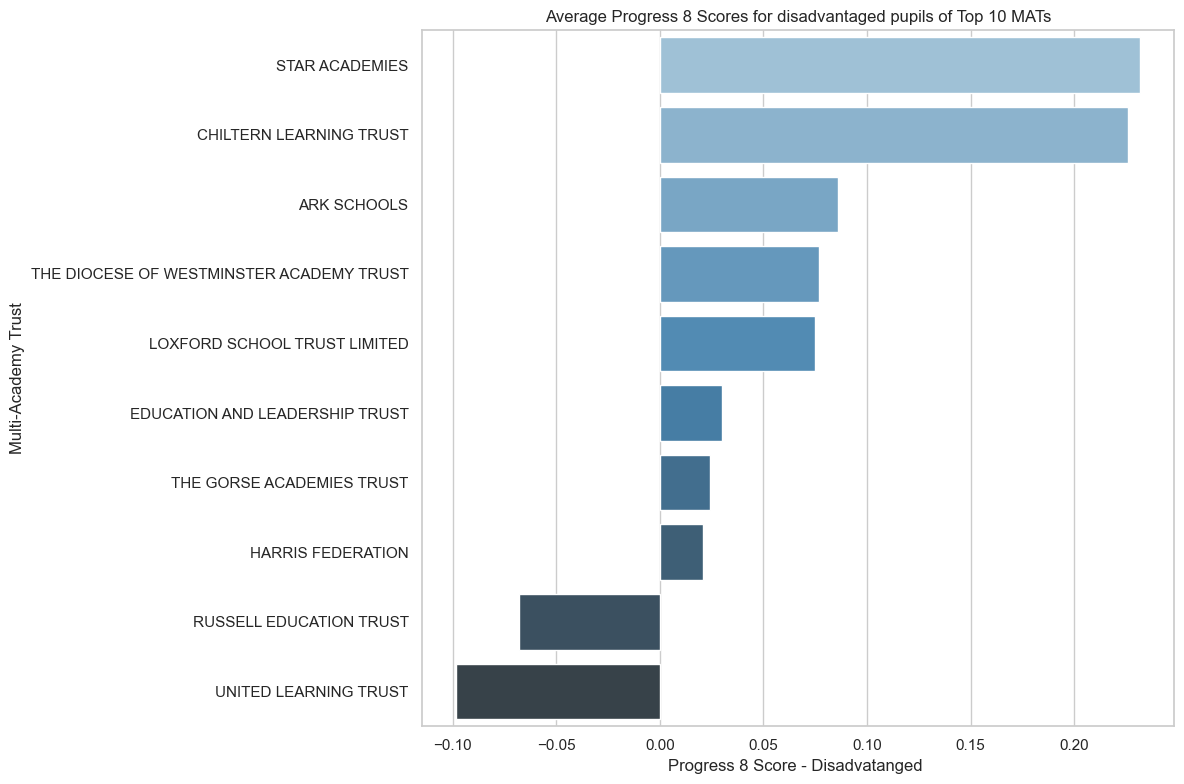
\includegraphics{P4DS_A2_Data_Analysis_Project_files/figure-pdf/cell-99-output-2.png}

\begin{Shaded}
\begin{Highlighting}[]
\CommentTok{\# Melt the DataFrame for easier plotting}
\NormalTok{top\_10\_MATs}\OperatorTok{=}\NormalTok{ MAT\_performance\_sorted.head(}\DecValTok{10}\NormalTok{)}
\NormalTok{prog8\_melted }\OperatorTok{=}\NormalTok{ top\_10\_MATs.melt(}
\NormalTok{    id\_vars}\OperatorTok{=}\StringTok{\textquotesingle{}Trust\_Name\textquotesingle{}}\NormalTok{, }
\NormalTok{    value\_vars}\OperatorTok{=}\NormalTok{[}\StringTok{\textquotesingle{}prog8\_score\_disadv\textquotesingle{}}\NormalTok{, }\StringTok{\textquotesingle{}prog8\_score\_nondisadv\textquotesingle{}}\NormalTok{],}
\NormalTok{    var\_name}\OperatorTok{=}\StringTok{\textquotesingle{}Group\textquotesingle{}}\NormalTok{,}
\NormalTok{    value\_name}\OperatorTok{=}\StringTok{\textquotesingle{}Progress8\_Score\textquotesingle{}}
\NormalTok{)}

\CommentTok{\# Replace group names for clarity}
\NormalTok{prog8\_melted[}\StringTok{\textquotesingle{}Group\textquotesingle{}}\NormalTok{] }\OperatorTok{=}\NormalTok{ prog8\_melted[}\StringTok{\textquotesingle{}Group\textquotesingle{}}\NormalTok{].}\BuiltInTok{map}\NormalTok{(\{}
    \StringTok{\textquotesingle{}prog8\_score\_disadv\textquotesingle{}}\NormalTok{: }\StringTok{\textquotesingle{}Disadvantaged\textquotesingle{}}\NormalTok{,}
    \StringTok{\textquotesingle{}prog8\_score\_nondisadv\textquotesingle{}}\NormalTok{: }\StringTok{\textquotesingle{}Non{-}Disadvantaged\textquotesingle{}}
\NormalTok{\})}

\CommentTok{\# Plot}
\NormalTok{plt.figure(figsize}\OperatorTok{=}\NormalTok{(}\DecValTok{14}\NormalTok{, }\DecValTok{8}\NormalTok{))}
\NormalTok{sns.barplot(}
\NormalTok{    x}\OperatorTok{=}\StringTok{\textquotesingle{}Trust\_Name\textquotesingle{}}\NormalTok{, }
\NormalTok{    y}\OperatorTok{=}\StringTok{\textquotesingle{}Progress8\_Score\textquotesingle{}}\NormalTok{, }
\NormalTok{    hue}\OperatorTok{=}\StringTok{\textquotesingle{}Group\textquotesingle{}}\NormalTok{, }
\NormalTok{    data}\OperatorTok{=}\NormalTok{prog8\_melted, }
\NormalTok{    palette}\OperatorTok{=}\StringTok{\textquotesingle{}Set1\textquotesingle{}}
\NormalTok{)}
\NormalTok{plt.title(}\StringTok{\textquotesingle{}Progress 8 Scores: Disadvantaged vs. Non{-}Disadvantaged Students\textquotesingle{}}\NormalTok{)}
\NormalTok{plt.xlabel(}\StringTok{\textquotesingle{}Multi{-}Academy Trust\textquotesingle{}}\NormalTok{)}
\NormalTok{plt.ylabel(}\StringTok{\textquotesingle{}Progress 8 Score\textquotesingle{}}\NormalTok{)}
\NormalTok{plt.legend(title}\OperatorTok{=}\StringTok{\textquotesingle{}Student Group\textquotesingle{}}\NormalTok{)}
\NormalTok{plt.xticks(rotation}\OperatorTok{=}\DecValTok{45}\NormalTok{)}
\NormalTok{plt.tight\_layout()}

\CommentTok{\#save the image in data folder}
\NormalTok{images\_dir }\OperatorTok{=} \StringTok{\textquotesingle{}images\textquotesingle{}}
\NormalTok{image\_path }\OperatorTok{=}\NormalTok{ os.path.join(images\_dir,}\StringTok{\textquotesingle{}Obj3\_Progress8 disadv vs advantaged in top 10 MATs.png\textquotesingle{}}\NormalTok{)}
\NormalTok{plt.savefig(image\_path)}

\NormalTok{plt.show()}
\end{Highlighting}
\end{Shaded}

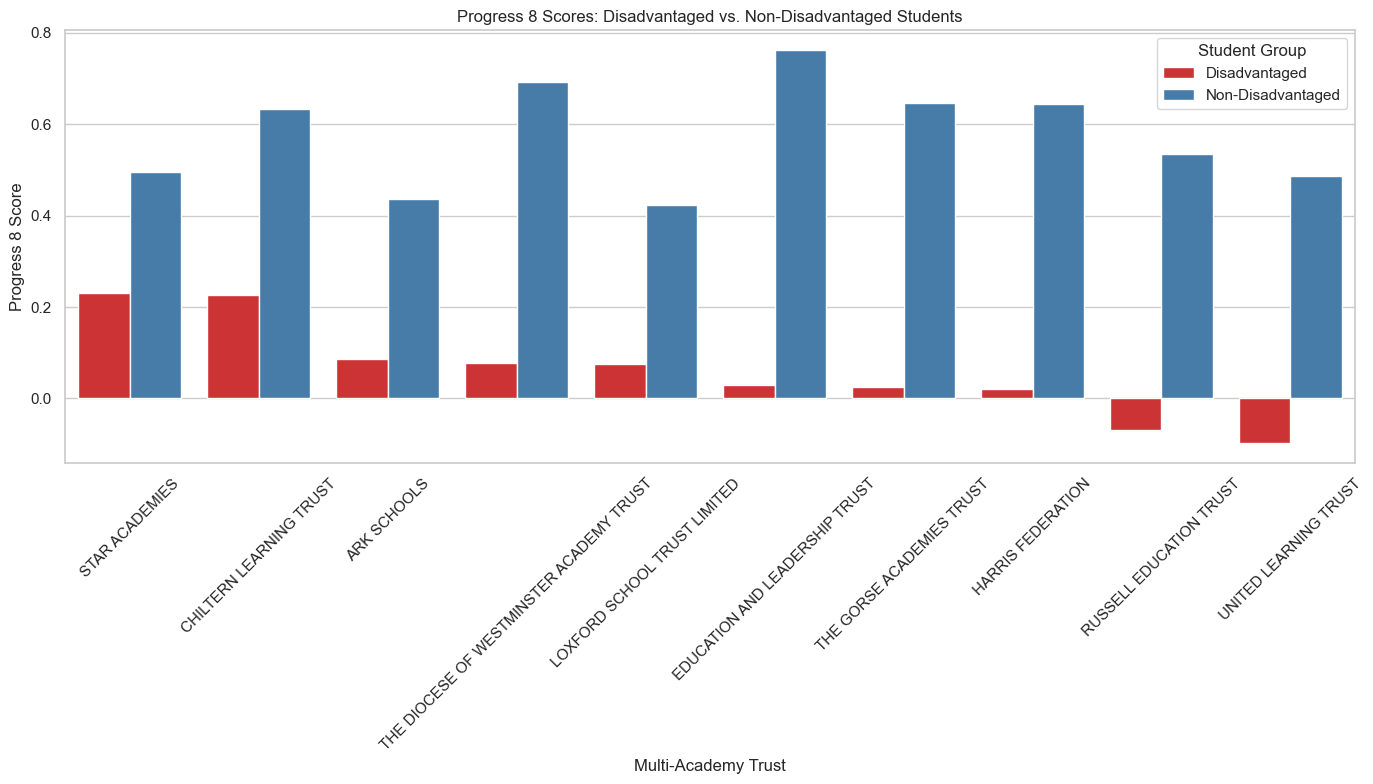
\includegraphics{P4DS_A2_Data_Analysis_Project_files/figure-pdf/cell-100-output-1.png}

Plot a scatterplot of MATs and average progress 8

\begin{Shaded}
\begin{Highlighting}[]
\NormalTok{plt.figure(figsize}\OperatorTok{=}\NormalTok{(}\DecValTok{10}\NormalTok{, }\DecValTok{6}\NormalTok{))}
\NormalTok{sns.scatterplot(}
\NormalTok{    x}\OperatorTok{=}\StringTok{\textquotesingle{}deprivation\_index\textquotesingle{}}\NormalTok{, }
\NormalTok{    y}\OperatorTok{=}\StringTok{\textquotesingle{}avg\_progress8\_score\textquotesingle{}}\NormalTok{, }
\NormalTok{    data}\OperatorTok{=}\NormalTok{top\_10\_MATs,}
\NormalTok{    s}\OperatorTok{=}\DecValTok{100}\NormalTok{,}
\NormalTok{    color}\OperatorTok{=}\StringTok{\textquotesingle{}green\textquotesingle{}}\NormalTok{,}
\NormalTok{    edgecolor}\OperatorTok{=}\StringTok{\textquotesingle{}black\textquotesingle{}}
\NormalTok{)}
\NormalTok{plt.title(}\StringTok{\textquotesingle{}Deprivation Index vs. Average Progress 8 Score\textquotesingle{}}\NormalTok{)}
\NormalTok{plt.xlabel(}\StringTok{\textquotesingle{}Index of Multiple Deprivation Decile\textquotesingle{}}\NormalTok{)}
\NormalTok{plt.ylabel(}\StringTok{\textquotesingle{}Average Progress 8 Score\textquotesingle{}}\NormalTok{)}
\NormalTok{plt.tight\_layout()}


\CommentTok{\# Annotate MAT names}
\ControlFlowTok{for}\NormalTok{ idx, row }\KeywordTok{in}\NormalTok{ top\_10\_MATs.iterrows():}
\NormalTok{    plt.text(row[}\StringTok{\textquotesingle{}deprivation\_index\textquotesingle{}}\NormalTok{]}\OperatorTok{+}\FloatTok{0.1}\NormalTok{, row[}\StringTok{\textquotesingle{}avg\_progress8\_score\textquotesingle{}}\NormalTok{]}\OperatorTok{+}\FloatTok{0.01}\NormalTok{, }
\NormalTok{             row[}\StringTok{\textquotesingle{}Trust\_Name\textquotesingle{}}\NormalTok{], fontsize}\OperatorTok{=}\DecValTok{9}\NormalTok{)}

\NormalTok{images\_dir }\OperatorTok{=} \StringTok{\textquotesingle{}images\textquotesingle{}}
\NormalTok{image\_path }\OperatorTok{=}\NormalTok{ os.path.join(images\_dir,}\StringTok{\textquotesingle{}Obj3\_Deprivation Index vs P8 top 10 MATS.png\textquotesingle{}}\NormalTok{)}
\NormalTok{plt.savefig(image\_path)}

\NormalTok{plt.show()}
\end{Highlighting}
\end{Shaded}

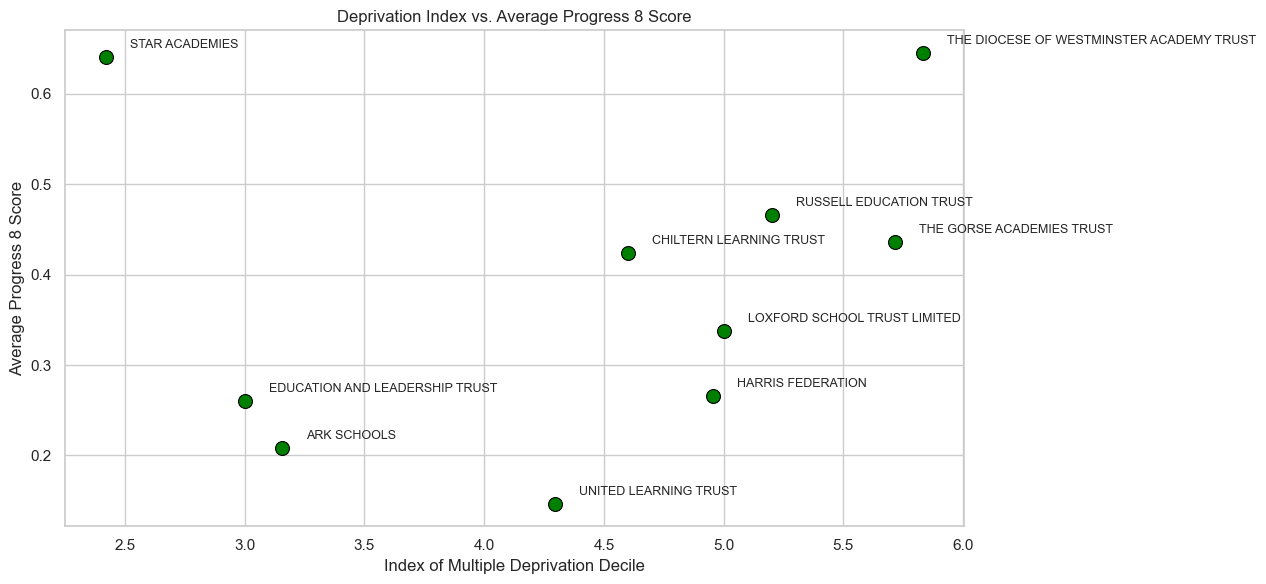
\includegraphics{P4DS_A2_Data_Analysis_Project_files/figure-pdf/cell-101-output-1.png}

Plot a scatter plor of MATs and progres 8 disadvantages

\begin{Shaded}
\begin{Highlighting}[]
\NormalTok{plt.figure(figsize}\OperatorTok{=}\NormalTok{(}\DecValTok{10}\NormalTok{, }\DecValTok{6}\NormalTok{))}
\NormalTok{sns.scatterplot(}
\NormalTok{    x}\OperatorTok{=}\StringTok{\textquotesingle{}deprivation\_index\textquotesingle{}}\NormalTok{, }
\NormalTok{    y}\OperatorTok{=}\StringTok{\textquotesingle{}prog8\_score\_disadv\textquotesingle{}}\NormalTok{, }
\NormalTok{    data}\OperatorTok{=}\NormalTok{top\_10\_MATs,}
\NormalTok{    s}\OperatorTok{=}\DecValTok{100}\NormalTok{,}
\NormalTok{    color}\OperatorTok{=}\StringTok{\textquotesingle{}green\textquotesingle{}}\NormalTok{,}
\NormalTok{    edgecolor}\OperatorTok{=}\StringTok{\textquotesingle{}black\textquotesingle{}}
\NormalTok{)}
\NormalTok{plt.title(}\StringTok{\textquotesingle{}Deprivation Index vs. Average Progress 8 Score\textquotesingle{}}\NormalTok{)}
\NormalTok{plt.xlabel(}\StringTok{\textquotesingle{}Index of Multiple Deprivation Decile\textquotesingle{}}\NormalTok{)}
\NormalTok{plt.ylabel(}\StringTok{\textquotesingle{}Progress 8 Score {-} Disadvantaged\textquotesingle{}}\NormalTok{)}
\NormalTok{plt.tight\_layout()}

\CommentTok{\# Annotate MAT names}
\ControlFlowTok{for}\NormalTok{ idx, row }\KeywordTok{in}\NormalTok{ top\_10\_MATs.iterrows():}
\NormalTok{    plt.text(row[}\StringTok{\textquotesingle{}deprivation\_index\textquotesingle{}}\NormalTok{]}\OperatorTok{+}\FloatTok{0.1}\NormalTok{, row[}\StringTok{\textquotesingle{}prog8\_score\_disadv\textquotesingle{}}\NormalTok{]}\OperatorTok{+}\FloatTok{0.01}\NormalTok{, }
\NormalTok{             row[}\StringTok{\textquotesingle{}Trust\_Name\textquotesingle{}}\NormalTok{], fontsize}\OperatorTok{=}\DecValTok{9}\NormalTok{)}


\NormalTok{images\_dir }\OperatorTok{=} \StringTok{\textquotesingle{}images\textquotesingle{}}
\NormalTok{image\_path }\OperatorTok{=}\NormalTok{ os.path.join(images\_dir,}\StringTok{\textquotesingle{}Obj3\_Progress8 Disadv vs Deprivation Index for Top 10 MATs.png\textquotesingle{}}\NormalTok{)}
\NormalTok{plt.savefig(image\_path)}

\NormalTok{plt.show()}
\end{Highlighting}
\end{Shaded}

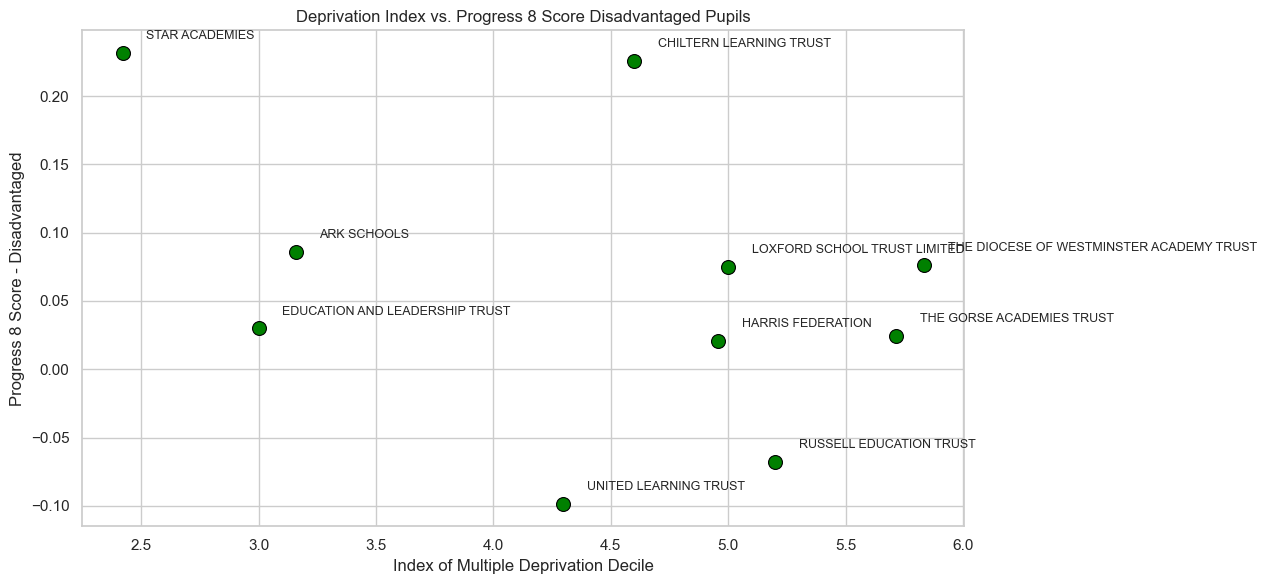
\includegraphics{P4DS_A2_Data_Analysis_Project_files/figure-pdf/cell-103-output-1.png}

Before we can analyse the correlation coefficients I would need to
standardise the data

\begin{Shaded}
\begin{Highlighting}[]


\CommentTok{\# Columns to standardise}
\NormalTok{corr\_columns }\OperatorTok{=}\NormalTok{ [}\StringTok{\textquotesingle{}avg\_progress8\_score\textquotesingle{}}\NormalTok{, }\StringTok{\textquotesingle{}prog8\_score\_disadv\textquotesingle{}}\NormalTok{, }
                \StringTok{\textquotesingle{}prog8\_score\_nondisadv\textquotesingle{}}\NormalTok{, }\StringTok{\textquotesingle{}deprivation\_index\textquotesingle{}}\NormalTok{, }\StringTok{\textquotesingle{}progress8\_gap\textquotesingle{}}\NormalTok{, }
                \StringTok{\textquotesingle{}attainment8\_gap\textquotesingle{}}\NormalTok{, }\StringTok{\textquotesingle{}maths\_gap\textquotesingle{}}\NormalTok{, }\StringTok{\textquotesingle{}english\_gap\textquotesingle{}}\NormalTok{, }\StringTok{\textquotesingle{}FiveGCSE\_gap\textquotesingle{}}\NormalTok{,}
                \StringTok{\textquotesingle{}school\_count\textquotesingle{}}\NormalTok{]}

\NormalTok{scaler }\OperatorTok{=}\NormalTok{ StandardScaler() }\CommentTok{\# this will give a mean of 0 and SD of 1}

\CommentTok{\#fiter data}
\NormalTok{top\_10\_MATs\_standardized }\OperatorTok{=}\NormalTok{ top\_10\_MATs.copy()}
\NormalTok{top\_10\_MATs\_standardized[corr\_columns] }\OperatorTok{=}\NormalTok{ scaler.fit\_transform(top\_10\_MATs[corr\_columns])}


\BuiltInTok{print}\NormalTok{(top\_10\_MATs\_standardized.head())}
\end{Highlighting}
\end{Shaded}

\begin{verbatim}
                                    Trust_Name  avg_progress8_score  \
975                             STAR ACADEMIES             1.586519   
219                    CHILTERN LEARNING TRUST             0.252807   
57                                 ARK SCHOOLS            -1.075069   
1096  THE DIOCESE OF WESTMINSTER ACADEMY TRUST             1.614075   
628               LOXFORD SCHOOL TRUST LIMITED            -0.279996   

      prog8_score_disadv  prog8_score_nondisadv  progress8_gap  \
975             1.684115              -0.725355      -1.680816   
219             1.629234               0.534547      -0.717045   
57              0.249948              -1.272304      -1.105799   
1096            0.160204               1.060226       0.670404   
628             0.143809              -1.393449      -1.122556   

      attainment8_gap  maths_gap  english_gap  FiveGCSE_gap  \
975         -1.044491  -1.314392    -0.789312     -1.534426   
219         -0.575425  -0.216238    -0.341835     -0.421951   
57          -1.082402  -0.343113    -0.589626     -0.542685   
1096         0.413372  -1.255853    -1.145190      0.206152   
628         -1.428343  -1.193430    -1.206268     -0.708694   

      deprivation_index  school_count  
975           -1.782039      0.575651  
219            0.162376     -0.745515  
57            -1.124507      0.575651  
1096           1.262959     -0.651146  
628            0.519322     -0.839884  
\end{verbatim}

\begin{Shaded}
\begin{Highlighting}[]
\CommentTok{\# Selecting rthe needed columns for correlation}
\NormalTok{corr\_columns }\OperatorTok{=}\NormalTok{ [}\StringTok{\textquotesingle{}avg\_progress8\_score\textquotesingle{}}\NormalTok{, }\StringTok{\textquotesingle{}prog8\_score\_disadv\textquotesingle{}}\NormalTok{, }
                \StringTok{\textquotesingle{}prog8\_score\_nondisadv\textquotesingle{}}\NormalTok{, }\StringTok{\textquotesingle{}deprivation\_index\textquotesingle{}}\NormalTok{, }\StringTok{\textquotesingle{}progress8\_gap\textquotesingle{}}\NormalTok{, }\StringTok{\textquotesingle{}attainment8\_gap\textquotesingle{}}\NormalTok{,}
       \StringTok{\textquotesingle{}maths\_gap\textquotesingle{}}\NormalTok{, }\StringTok{\textquotesingle{}english\_gap\textquotesingle{}}\NormalTok{, }\StringTok{\textquotesingle{}FiveGCSE\_gap\textquotesingle{}}\NormalTok{,}
                \StringTok{\textquotesingle{}school\_count\textquotesingle{}}\NormalTok{]}

\CommentTok{\# Compute the correlation matrix}
\NormalTok{corr\_matrix }\OperatorTok{=}\NormalTok{ top\_10\_MATs[corr\_columns].corr()}

\CommentTok{\# Plot the heatmap}
\NormalTok{plt.figure(figsize}\OperatorTok{=}\NormalTok{(}\DecValTok{8}\NormalTok{, }\DecValTok{6}\NormalTok{))}
\NormalTok{sns.heatmap(corr\_matrix, annot}\OperatorTok{=}\VariableTok{True}\NormalTok{, cmap}\OperatorTok{=}\StringTok{\textquotesingle{}coolwarm\textquotesingle{}}\NormalTok{, fmt}\OperatorTok{=}\StringTok{".2f"}\NormalTok{, linewidths}\OperatorTok{=}\FloatTok{0.5}\NormalTok{)}
\NormalTok{plt.title(}\StringTok{\textquotesingle{}Correlation Matrix of Performance Metrics for Top 10 MATs\textquotesingle{}}\NormalTok{)}
\NormalTok{plt.tight\_layout()}

\CommentTok{\#save the file in the data folder}
\NormalTok{images\_dir }\OperatorTok{=} \StringTok{\textquotesingle{}images\textquotesingle{}}
\NormalTok{image\_path }\OperatorTok{=}\NormalTok{ os.path.join(images\_dir,}\StringTok{\textquotesingle{}Obj3\_Correlation Matrix top 10 MATS.png\textquotesingle{}}\NormalTok{)}
\NormalTok{plt.savefig(image\_path)}

\NormalTok{plt.show()}
\end{Highlighting}
\end{Shaded}

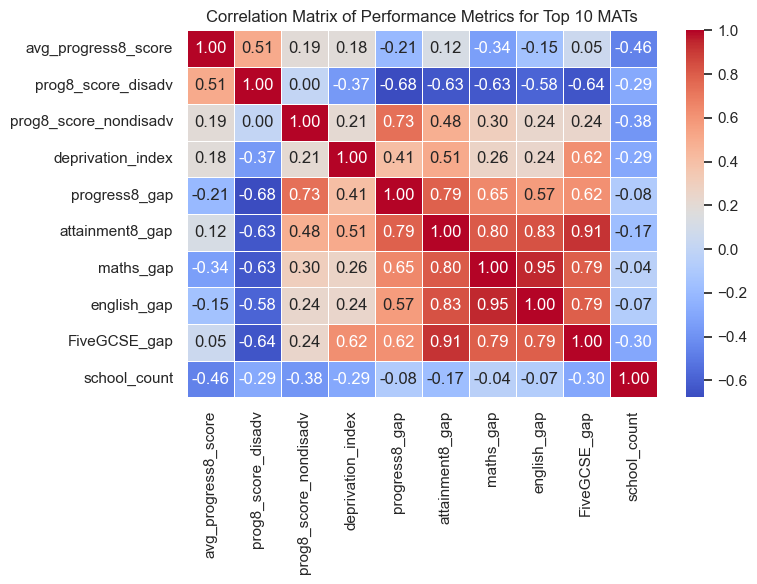
\includegraphics{P4DS_A2_Data_Analysis_Project_files/figure-pdf/cell-105-output-1.png}

\section{Project Outcome}\label{project-outcome}

\subsection{Overview of Results}\label{overview-of-results}

Objective 1: Evaluate National Disparities in Educational Performance

There significant gaps between non-disadvantaged and disadvantaged
pupils including attainment 8, progress 8, Maths, English and strong
passes in both. Disadvantaged pupils lag behind by approximately 1.45
GCSE grades per subject and have an attainment 8 gap of 11.6 points.
Their Progress 8 scores are 0.6 grades lower across subjects than their
peers, suggesting significant performance gaps.

Objective 2: Identify and Analyse Outlier Schools in Positive Progress 8
of Disadvantaged Pupils

Schools excelling in progress 8 for disadvantaged students, tend to
support all students very well and have a strong positive correlation
(0.85) between overall and disadvantaged pupils. Funding has a negative
correlation with Progress 8 scores for disadvantaged pupils, and could
be investigated further.

Objective 3: Identify and Evaluate Top Performing Multi-Academy Trusts
(MATs)

High performing MAT have shown a strong positive correlation (0.51)
between progress 8 scores for disadvantaged students and overall scores.
Although socio-economic factors negatively correlate (-0.37) with
progress, for high performing MATs this hasn't been seen to be a
barrier; Star Academies for example is one of the highest performing
MATs in the country, yet faces the highest deprivation average of all
MATs, suggesting a robust pedagogical strategy and governance to run its
schools. Such high performing MATs are good at closing the gap (smallest
is 0.264 progress 8) between disadvantaged and advantaged students,
demonstrating efficient use of funding and better equity.

\section{Objective 1: Evaluate National Disparities in Educational
Performance Between Advantaged and Disadvantaged
Pupils}\label{objective-1-evaluate-national-disparities-in-educational-performance-between-advantaged-and-disadvantaged-pupils}

\textbf{Explaination of Results:}

There are positive gaps in all categories measured between advantaged
and disadvantaged pupils, confirming that nationally, isadvanteged
pupils are behind in every academic measure.

\textbf{Attainment 8 Gap:}

\begin{itemize}
\item
  Attainment 8 Disadvantaged: 40.22
\item
  Attainment 8 Non-Disadvantaged: 51.83
\item
  Attainment 8 Gap: 11.61
\end{itemize}

Analysis: The attainment 8 gap of 11.6 points between disadvantaged and
advantaged pupils nationally, suggest approximately 1.45 GCSE grades
lower per subject for disadvantaged stidents (11.61/8 = 1.45125 - as
each subject is given a point based on the GCSE grade e.g.~grade 9 = 9
points).

\textbf{Progress 8 Gap:}

\begin{itemize}
\item
  Progress 8 Disadvantaged: -0.47
\item
  Progress 8 Non-Disadvantaged: 0.13
\item
  Progress 8 Gap: 0.60
\end{itemize}

Analysis: Progress 8 gap of 0.60 that disadvantaged pupils are making
0.6 grades less progress across 8 subjects between keystage 2 and
keystage 4 nationally. This would amount to 0.075 grade point less in
each of the 8 subjects (0.60/8=0.0.075)

\textbf{Subject Specific Gaps:}

\begin{itemize}
\item
  Maths Disadvantaged: -0.44
\item
  Maths Non-Disadvantaged: 0.11
\item
  Maths Gap: 0.55
\item
  English Disadvantaged: -0.46
\item
  English Non-Disadvantaged: 0.12
\item
  English Gap: 0.58
\end{itemize}

Analysis: Maths gap of 0.55 and English gap of 0.58 suggest, nationally,
disadvanted students are underperforming or making 0.55 grade less
progress in maths and 0.58 less progress in English, between keystage 2
and keystage 4 nationally.

\textbf{Perventage 9-5 Gap:}

\begin{itemize}
\item
  Percentage Disadvanted EngMaths\_95: 28.09
\item
  Percentage Nondisadv Student EngMaths\_95: 50.01
\item
  Percentage\_95 Gap: 21.92
\end{itemize}

Analysis: Signficcant gap of 21.92 percentage points nationally between
disadvatanged and advantaged students achieving grade 5 or above in
English and Maths, suggests this needs to be addressed.

\subsubsection{Visualisation}\label{visualisation}

\textbf{Distribution of Progress 8 Scores}

The histrogram showes an approximately normal distribution, as expected,
since the results are standardised by exam boards. Most sudents would
therfore have a progress 8 score of 0, with 68\% of students falling
within +1 or -1 standard deviations from the mean and 95\% falling
within +2 or -2 standard deviations from the mean.

\begin{figure}[H]

{\centering 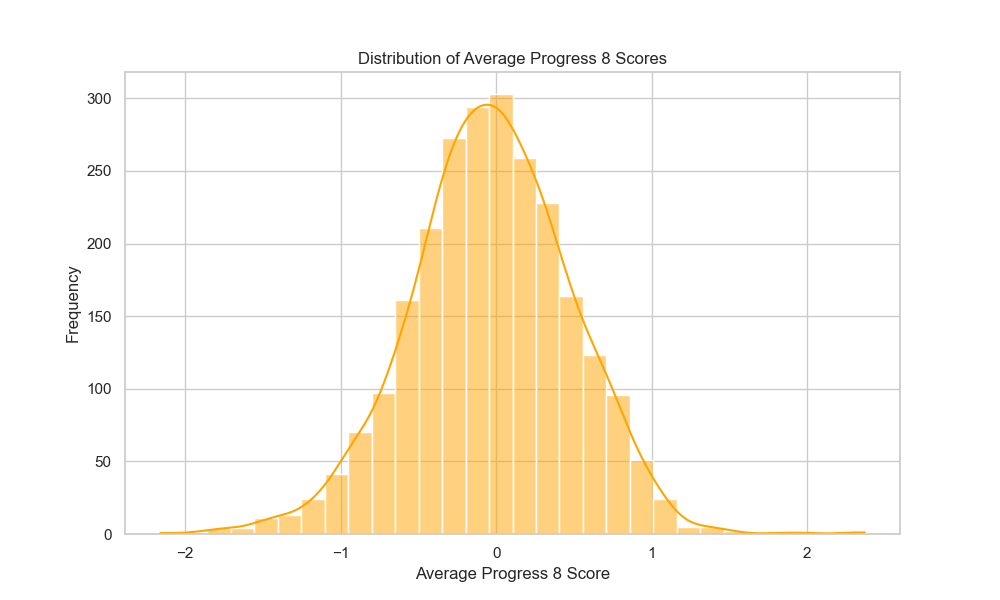
\includegraphics{P4DS_A2_Data_Analysis_Project_files/figure-pdf/cell-191-1-Obj1_progress8_distribution_nationally.png}

}

\caption{Obj1\_progress8\_distribution\_nationally.png}

\end{figure}%

\textbf{Progess 8 and Attainment 8 Box Plots}

Both box plots show disadvantaged students under performing. For
progress 8, disadvatanged students have a negative progress 8 of -0.49
median score while advtanged students have a positive median score of
0.13, suggesting significant disparity. Both have a similar range and
interquratile range with a number of outliers. For attainment 8, the gap
and distribution is as expected given the results.

\begin{figure}[H]

{\centering 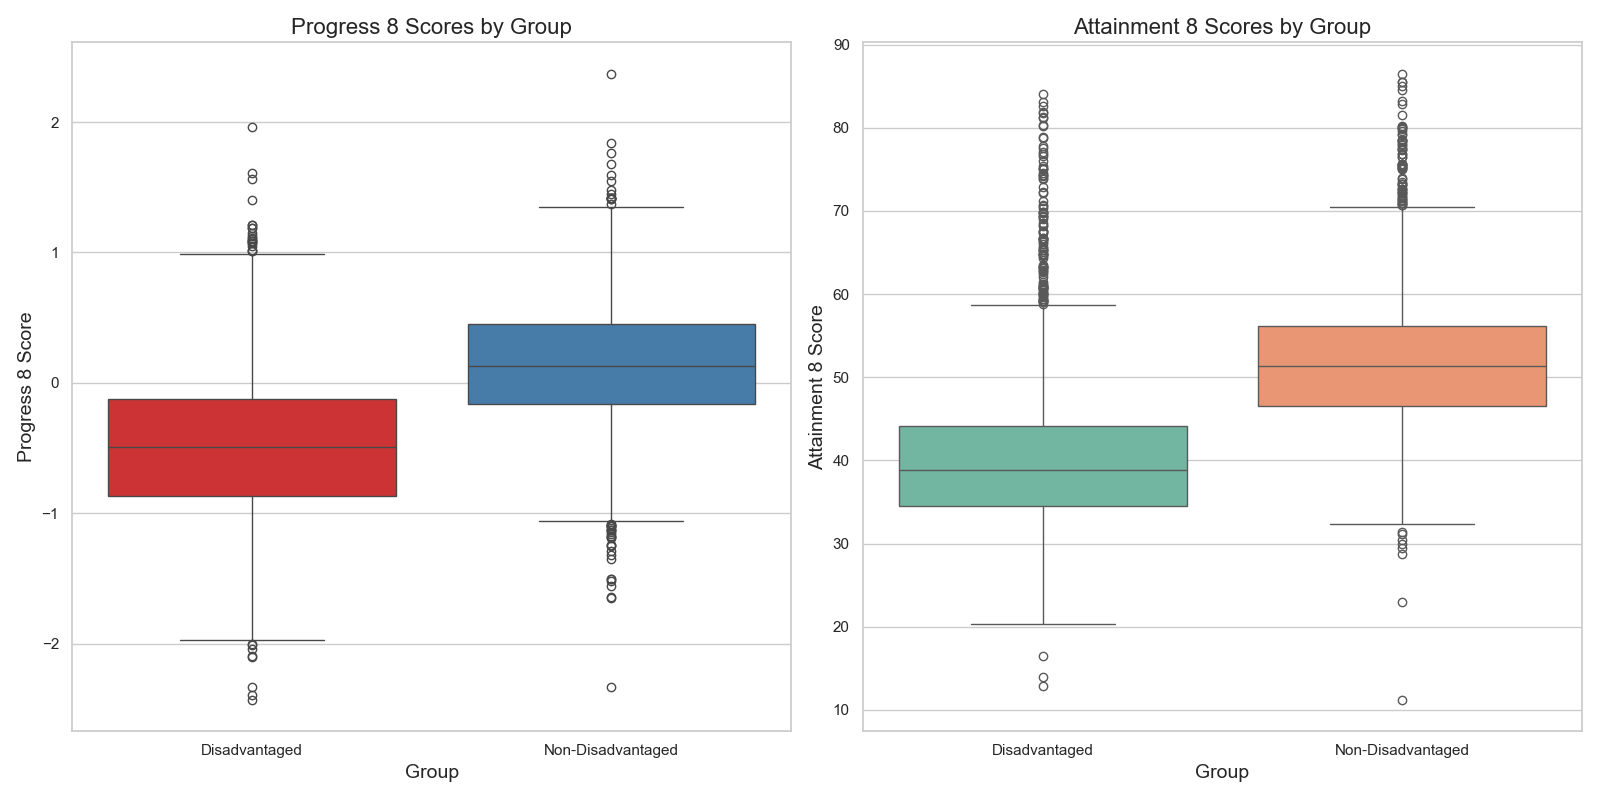
\includegraphics{P4DS_A2_Data_Analysis_Project_files/figure-pdf/cell-191-3-progress8_attainment8_boxplot.png}

}

\caption{progress8\_attainment8\_boxplot.png}

\end{figure}%

\textbf{Percentage English and Mathematics Five Plus Box Plots}

\begin{longtable}[]{@{}
  >{\raggedright\arraybackslash}p{(\columnwidth - 14\tabcolsep) * \real{0.2800}}
  >{\raggedright\arraybackslash}p{(\columnwidth - 14\tabcolsep) * \real{0.1200}}
  >{\raggedright\arraybackslash}p{(\columnwidth - 14\tabcolsep) * \real{0.1333}}
  >{\raggedright\arraybackslash}p{(\columnwidth - 14\tabcolsep) * \real{0.1333}}
  >{\raggedright\arraybackslash}p{(\columnwidth - 14\tabcolsep) * \real{0.0800}}
  >{\raggedright\arraybackslash}p{(\columnwidth - 14\tabcolsep) * \real{0.0800}}
  >{\raggedright\arraybackslash}p{(\columnwidth - 14\tabcolsep) * \real{0.0800}}
  >{\raggedright\arraybackslash}p{(\columnwidth - 14\tabcolsep) * \real{0.0933}}@{}}
\toprule\noalign{}
\begin{minipage}[b]{\linewidth}\raggedright
Maths Scores Summary
\end{minipage} & \begin{minipage}[b]{\linewidth}\raggedright
Median
\end{minipage} & \begin{minipage}[b]{\linewidth}\raggedright
Q1 (25\%)
\end{minipage} & \begin{minipage}[b]{\linewidth}\raggedright
Q3 (75\%)
\end{minipage} & \begin{minipage}[b]{\linewidth}\raggedright
IQR
\end{minipage} & \begin{minipage}[b]{\linewidth}\raggedright
Min
\end{minipage} & \begin{minipage}[b]{\linewidth}\raggedright
Max
\end{minipage} & \begin{minipage}[b]{\linewidth}\raggedright
Range
\end{minipage} \\
\midrule\noalign{}
\endhead
\bottomrule\noalign{}
\endlastfoot
Disadvantaged & -0.47 & -0.79 & -0.12 & 0.67 & -2.55 & 2.48 & 5.03 \\
Non-Disadvantaged & 0.11 & -0.20 & 0.42 & 0.62 & -1.65 & 2.95 & 4.60 \\
\end{longtable}

\begin{longtable}[]{@{}
  >{\raggedright\arraybackslash}p{(\columnwidth - 14\tabcolsep) * \real{0.2895}}
  >{\raggedright\arraybackslash}p{(\columnwidth - 14\tabcolsep) * \real{0.1184}}
  >{\raggedright\arraybackslash}p{(\columnwidth - 14\tabcolsep) * \real{0.1316}}
  >{\raggedright\arraybackslash}p{(\columnwidth - 14\tabcolsep) * \real{0.1316}}
  >{\raggedright\arraybackslash}p{(\columnwidth - 14\tabcolsep) * \real{0.0789}}
  >{\raggedright\arraybackslash}p{(\columnwidth - 14\tabcolsep) * \real{0.0789}}
  >{\raggedright\arraybackslash}p{(\columnwidth - 14\tabcolsep) * \real{0.0789}}
  >{\raggedright\arraybackslash}p{(\columnwidth - 14\tabcolsep) * \real{0.0921}}@{}}
\toprule\noalign{}
\begin{minipage}[b]{\linewidth}\raggedright
English Scores Summary
\end{minipage} & \begin{minipage}[b]{\linewidth}\raggedright
Median
\end{minipage} & \begin{minipage}[b]{\linewidth}\raggedright
Q1 (25\%)
\end{minipage} & \begin{minipage}[b]{\linewidth}\raggedright
Q3 (75\%)
\end{minipage} & \begin{minipage}[b]{\linewidth}\raggedright
IQR
\end{minipage} & \begin{minipage}[b]{\linewidth}\raggedright
Min
\end{minipage} & \begin{minipage}[b]{\linewidth}\raggedright
Max
\end{minipage} & \begin{minipage}[b]{\linewidth}\raggedright
Range
\end{minipage} \\
\midrule\noalign{}
\endhead
\bottomrule\noalign{}
\endlastfoot
Disadvantaged & -0.50 & -0.90 & -0.08 & 0.82 & -3.06 & 2.19 & 5.25 \\
Non-Disadvantaged & 0.11 & -0.20 & 0.44 & 0.64 & -2.31 & 2.33 & 4.64 \\
\end{longtable}

Both Maths and English have a negative median of -0.47 and -0.50 which
is very concerning, given this is a national pattern, showing progress
made by students between keystage 2 and keystage 4. English has a wider
interquartile range for disadvantaged students, suggesting more
variability. In both subjects, there is a greater difference between the
minimum values, then between the maximum values, suggesting the
disadvatnaged students will significiantly underperform than over
perform.

\begin{figure}[H]

{\centering 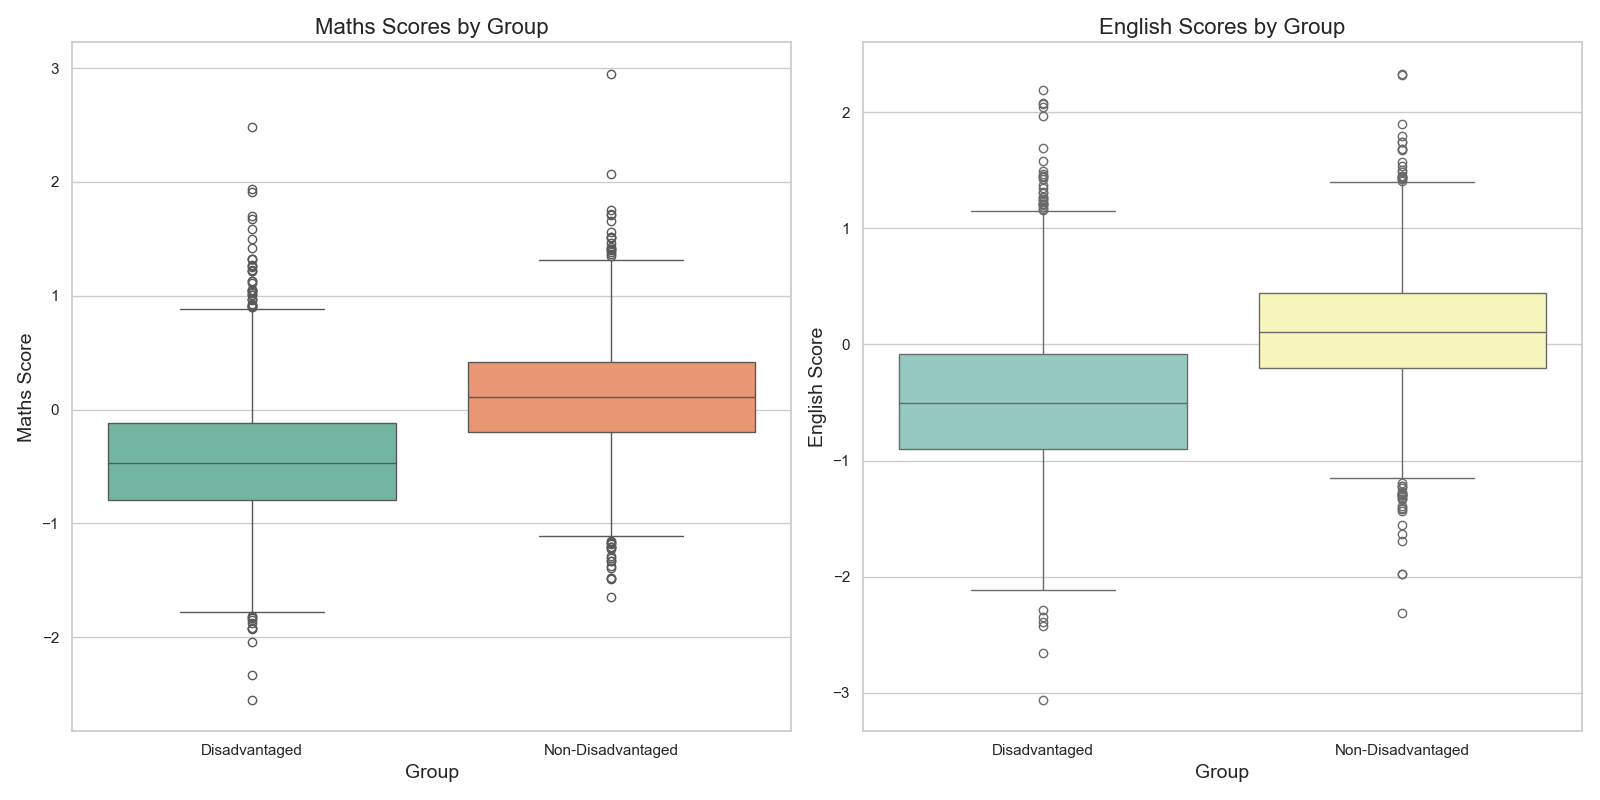
\includegraphics{P4DS_A2_Data_Analysis_Project_files/figure-pdf/cell-191-2-maths_english_scores_boxplot.png}

}

\caption{maths\_english\_scores\_boxplot.png}

\end{figure}%

\subsection{Objective 2 Identify and Analyse Outlier Schools in Positive
Progress 8 of Disadavantaged
Pupils}\label{objective-2-identify-and-analyse-outlier-schools-in-positive-progress-8-of-disadavantaged-pupils}

\subsubsection{Explanation of Results}\label{explanation-of-results}

Outlier schools for progress 8 were identified and then further
categories as:

\begin{enumerate}
\def\labelenumi{\alph{enumi})}
\item
  Schools which are outliers only for non-disadvantaged pupils
\item
  Schools which are outliers only for disadvantaged pupils
\item
  schools which are outliers for both non-disadvantaged and
  disadvantaged
\end{enumerate}

\begin{itemize}
\tightlist
\item
  Overall schools which are outliers in both categories will do
  significantly better for disadvantaged pupils.
\item
  There is also a higher correlation (0.85) between progress 8
  disadvantaged pupils and progress 8 in general, suggesting success
  breeds success.
\item
  Unexpectedly, funding (FSM(-0.45), total (-0.48) and pupil premium
  (-0.45)) all have negative correlation with progress 8 disadvantaged.
  This would need to be explored further as the range of the funding may
  be very small, and not being a good measure of proportionality.
\item
  Small postitive correlation of progress 8 disadvantaged with
  percentage of disadvantage pupils (0.19) suggest disadvantaged pupils
  may do better where there are more such pupils.
\item
  Index of multiple deprivation - has a negative correlation, suggesting
  lower values of the index ie. deprivation decreased, progress9
  disadvantaged pupils will decline slightly, suggesting disadvantaged
  pupils' performance is expected to decrease when there is more
  deprivation.
\end{itemize}

\textbf{Visualisation}

Heatmap provides insights into outlier schools in areas such as progress
8 score, funding, deprivation index etc.

\begin{figure}[H]

{\centering 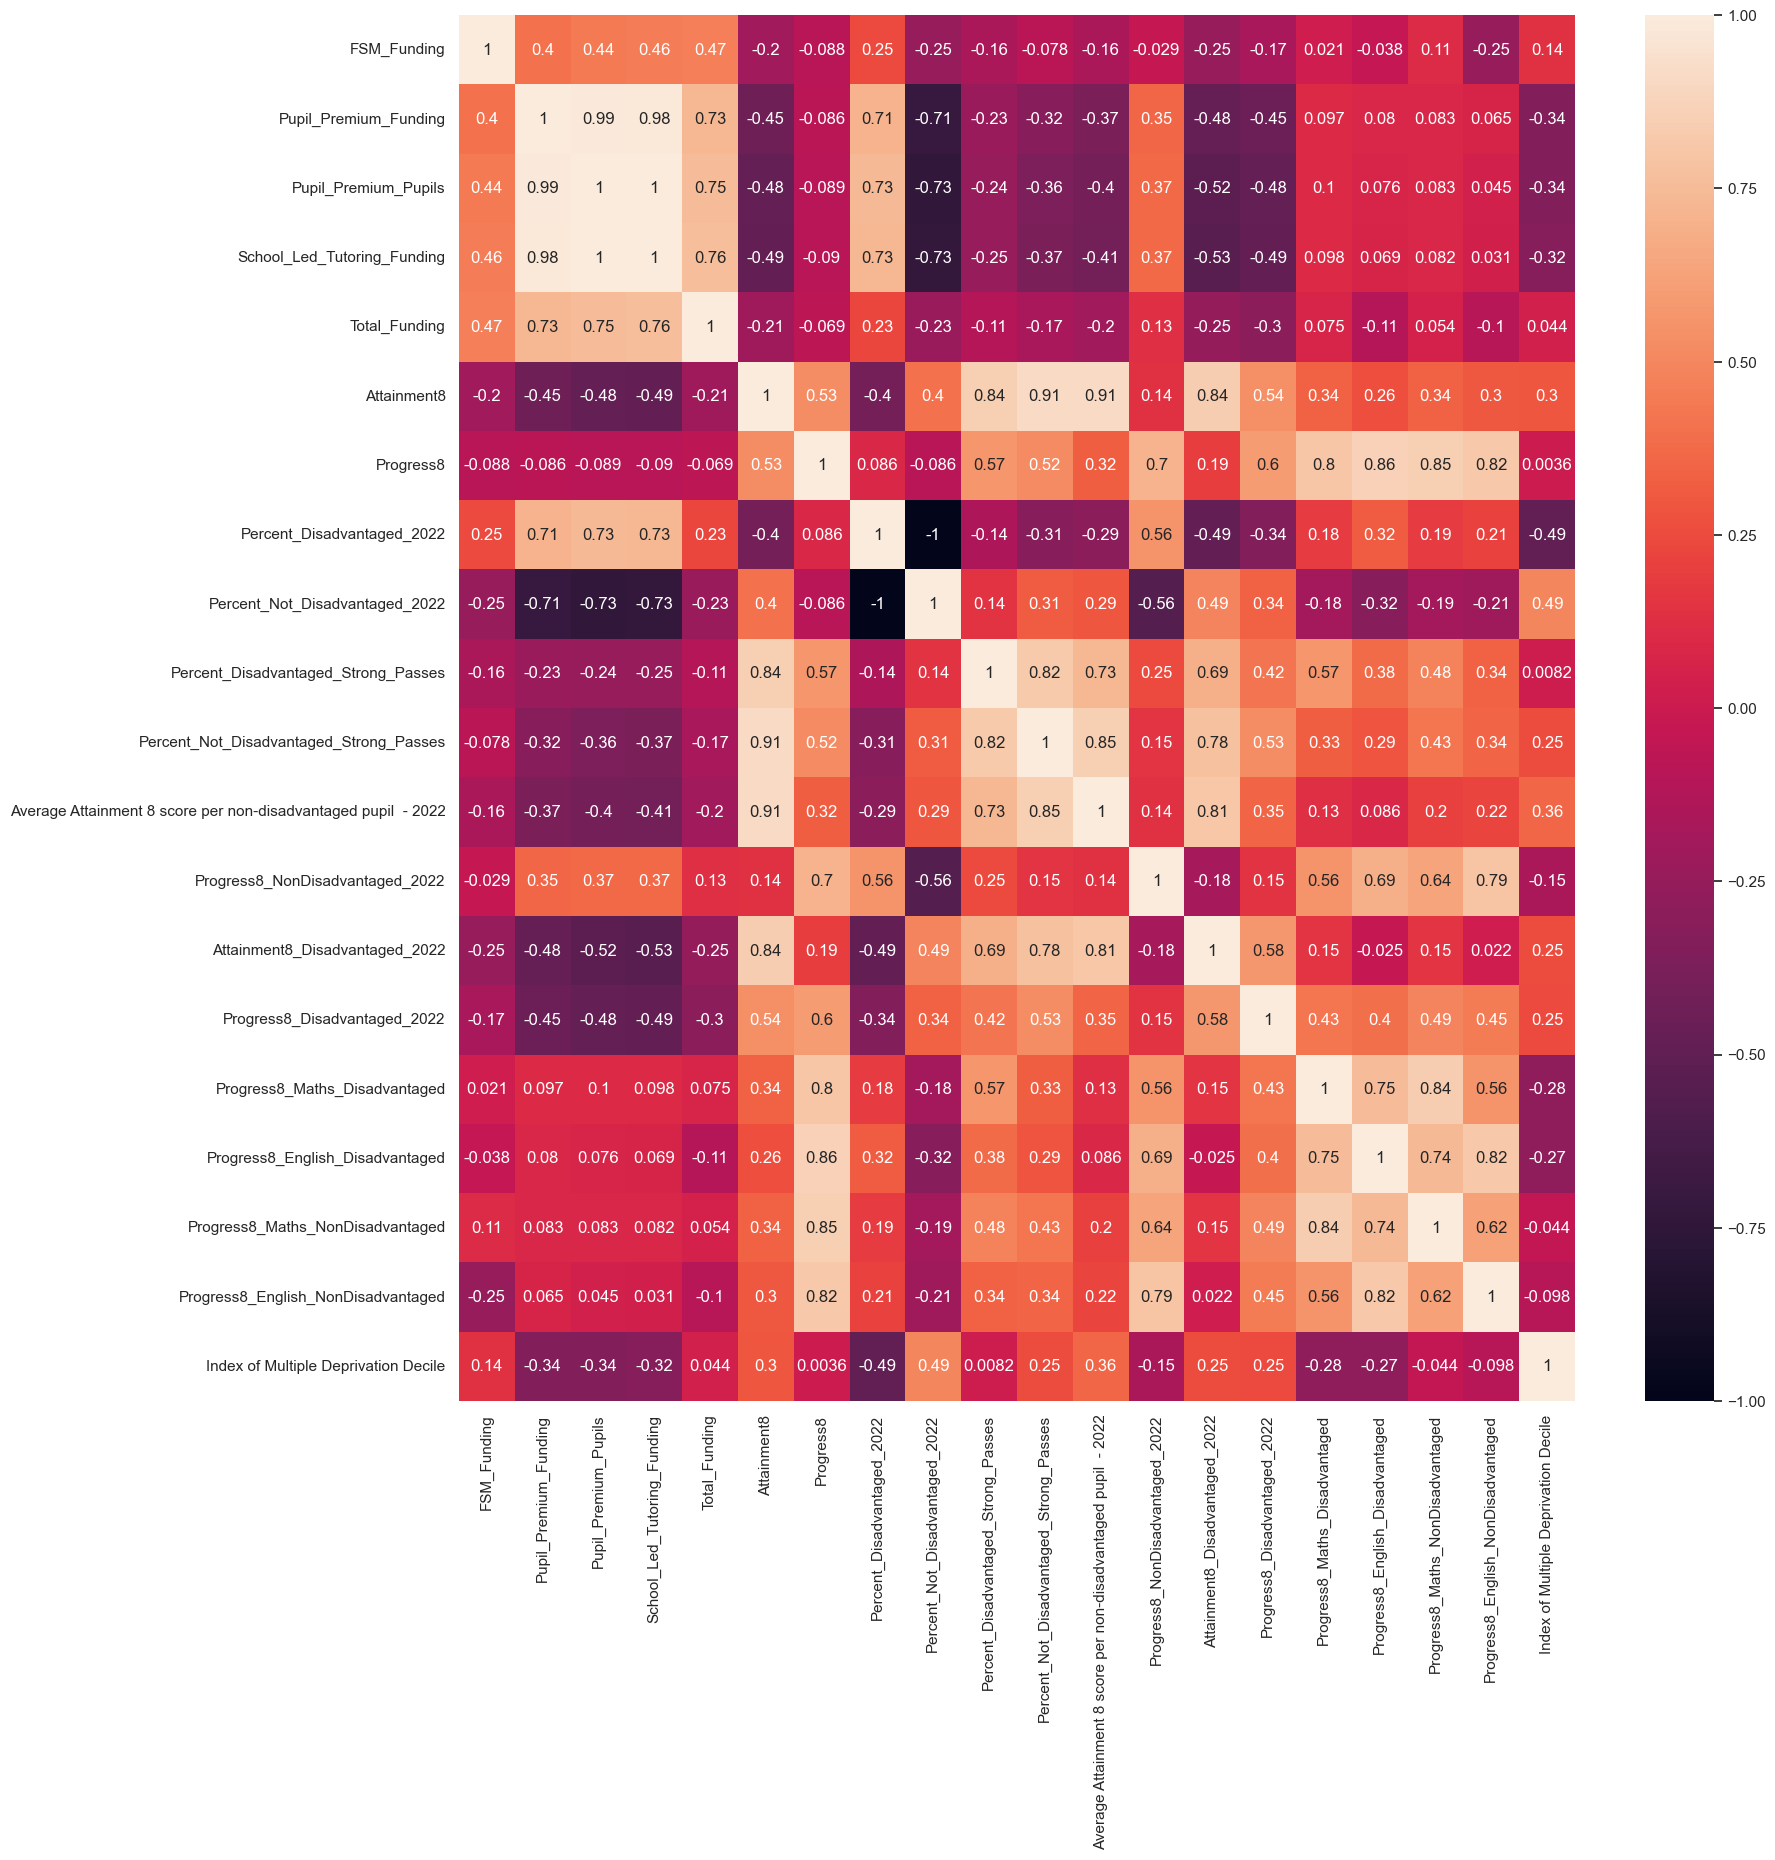
\includegraphics{P4DS_A2_Data_Analysis_Project_files/figure-pdf/cell-193-2-obj2_heatmap of outlier schools.png}

}

\caption{obj2\_heatmap of outlier schools.png}

\end{figure}%

\textbf{Summary Statistics for `Index of Multiple Deprivation Decile' by
`Outlier\_Category'} \textbar{} Outlier\_Category \textbar{} Median
\textbar{} Q1 (25\%) \textbar{} Q3 (75\%) \textbar{} IQR \textbar{} Min
\textbar{} Max \textbar{} Range \textbar{}
\textbar----------------------\textbar------------\textbar--------------\textbar--------------\textbar---------\textbar---------\textbar---------\textbar-----------\textbar{}
\textbar{} Both \textbar{} 7.0 \textbar{} 4.5 \textbar{} 8.50 \textbar{}
4.00 \textbar{} 1.0 \textbar{} 10.0 \textbar{} 9.0 \textbar{} \textbar{}
None \textbar{} 6.0 \textbar{} 3.0 \textbar{} 8.00 \textbar{} 5.00
\textbar{} 1.0 \textbar{} 10.0 \textbar{} 9.0 \textbar{} \textbar{}
Only\_Disadv \textbar{} 4.5 \textbar{} 3.0 \textbar{} 7.00 \textbar{}
4.00 \textbar{} 1.0 \textbar{} 9.0 \textbar{} 8.0 \textbar{} \textbar{}
Only\_NonDisadv \textbar{} 3.0 \textbar{} 2.0 \textbar{} 4.25 \textbar{}
2.25 \textbar{} 1.0 \textbar{} 8.0 \textbar{} 7.0 \textbar{}

Outlier schools only in progres 8 for only non-disadvantaged students,
stand out as having a significanlty lower median of deprivation index,
suggesting non-disadvantaged students tend to come from more deprived
areas in such schools. This could be due to more focused support given
they would stand out and be top of their school.

\begin{figure}[H]

{\centering 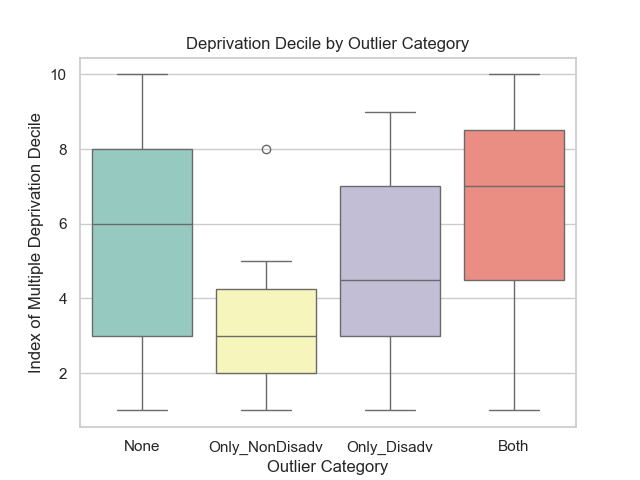
\includegraphics{P4DS_A2_Data_Analysis_Project_files/figure-pdf/cell-193-1-Obj2_Deprivation_by_Outlier_Category.png}

}

\caption{Obj2\_Deprivation\_by\_Outlier\_Category.png}

\end{figure}%

\textbf{Summary Statistics for `Progress8' by `Outlier\_Category'}
\textbar{} Outlier\_Category \textbar{} Median \textbar{} Q1 (25\%)
\textbar{} Q3 (75\%) \textbar{} IQR \textbar{} Min \textbar{} Max
\textbar{} Range \textbar{}
\textbar-----------------\textbar--------\textbar----------\textbar----------\textbar-----\textbar-----\textbar-----\textbar-------\textbar{}
\textbar{} Both \textbar{} 1.450 \textbar{} 1.1950 \textbar{} 2.140
\textbar{} 0.9450 \textbar{} 0.81 \textbar{} 2.37 \textbar{} 1.56
\textbar{} \textbar{} None \textbar{} -0.040 \textbar{} -0.3600
\textbar{} 0.290 \textbar{} 0.6500 \textbar{} -2.16 \textbar{} 1.83
\textbar{} 3.99 \textbar{} \textbar{} Only\_Disadv \textbar{} 0.955
\textbar{} 0.8500 \textbar{} 1.070 \textbar{} 0.2200 \textbar{} 0.25
\textbar{} 1.38 \textbar{} 1.13 \textbar{} \textbar{} Only\_NonDisadv
\textbar{} 1.085 \textbar{} 0.9375 \textbar{} 1.125 \textbar{} 0.1875
\textbar{} 0.61 \textbar{} 1.49 \textbar{} 0.88 \textbar{}

Non positive outlier schools are are expected nearing 0; the minor
difference may be due to negative outlier schools being included in that
group. Schools which are outliers in both categories are much better
performing with highest median and maximum score.

\begin{figure}[H]

{\centering \includegraphics{attachment:Obj2_Progress8\%20by\%20Outlier\%20Category.png}

}

\caption{Obj2\_Progress8 by Outlier Category.png}

\end{figure}%

\textbf{Summary Statistics for `Progress8\_Disadvantaged\_2022' by
`Outlier\_Category':}

\begin{longtable}[]{@{}
  >{\raggedright\arraybackslash}p{(\columnwidth - 14\tabcolsep) * \real{0.2537}}
  >{\raggedright\arraybackslash}p{(\columnwidth - 14\tabcolsep) * \real{0.1194}}
  >{\raggedright\arraybackslash}p{(\columnwidth - 14\tabcolsep) * \real{0.1493}}
  >{\raggedright\arraybackslash}p{(\columnwidth - 14\tabcolsep) * \real{0.1493}}
  >{\raggedright\arraybackslash}p{(\columnwidth - 14\tabcolsep) * \real{0.0746}}
  >{\raggedright\arraybackslash}p{(\columnwidth - 14\tabcolsep) * \real{0.0746}}
  >{\raggedright\arraybackslash}p{(\columnwidth - 14\tabcolsep) * \real{0.0746}}
  >{\raggedright\arraybackslash}p{(\columnwidth - 14\tabcolsep) * \real{0.1045}}@{}}
\toprule\noalign{}
\begin{minipage}[b]{\linewidth}\raggedright
Outlier\_Category
\end{minipage} & \begin{minipage}[b]{\linewidth}\raggedright
Median
\end{minipage} & \begin{minipage}[b]{\linewidth}\raggedright
Q1 (25\%)
\end{minipage} & \begin{minipage}[b]{\linewidth}\raggedright
Q3 (75\%)
\end{minipage} & \begin{minipage}[b]{\linewidth}\raggedright
IQR
\end{minipage} & \begin{minipage}[b]{\linewidth}\raggedright
Min
\end{minipage} & \begin{minipage}[b]{\linewidth}\raggedright
Max
\end{minipage} & \begin{minipage}[b]{\linewidth}\raggedright
Range
\end{minipage} \\
\midrule\noalign{}
\endhead
\bottomrule\noalign{}
\endlastfoot
Both & 1.40 & 1.19 & 1.585 & 0.395 & 1.01 & 1.96 & 0.95 \\
None & -0.50 & -0.87 & -0.140 & 0.730 & -2.43 & 0.99 & 3.42 \\
Only\_Disadv & 1.09 & 1.07 & 1.125 & 0.055 & 1.01 & 1.21 & 0.20 \\
Only\_NonDisadv & 0.60 & 0.51 & 0.775 & 0.265 & 0.22 & 0.99 & 0.77 \\
\end{longtable}

Similar to before, disadvantaged pupils do better in schools which are
outliers in both categories. Only disadvataged outlier schools have a
very small IQR, suggesting an excellent level of consistency and low
variability.

\begin{figure}[H]

{\centering \includegraphics{attachment:Obj2_Progress8\%20of\%20Disadvantaged\%20Pupils\%20by\%20Outlier\%20Category.png}

}

\caption{Obj2\_Progress8 of Disadvantaged Pupils by Outlier
Category.png}

\end{figure}%

\subsection{Objective 3 Identify and evaluate the top performing
multi-academy trusts in supporting disadvantaged
pupils}\label{objective-3-identify-and-evaluate-the-top-performing-multi-academy-trusts-in-supporting-disadvantaged-pupils}

\subsubsection{Explanation of Results}\label{explanation-of-results-1}

Summary:

\begin{longtable}[]{@{}ll@{}}
\toprule\noalign{}
Variable & Correlation with prog8\_score\_disadv \\
\midrule\noalign{}
\endhead
\bottomrule\noalign{}
\endlastfoot
avg\_progress8\_score & +0.51 \\
deprivation\_index & -0.37 \\
progress8\_gap & -0.68 \\
maths\_gap & -0.63 \\
english\_gap & -0.58 \\
attainment8\_gap & -0.63 \\
FiveGCSE\_gap & -0.64 \\
school\_count & -0.29 \\
\end{longtable}

Explaination:

\begin{itemize}
\item
  Strong positive correlation between the overall average Progress 8
  score and the Progress 8 score for disadvantaged students shows, MATS
  that tend to perform well in progress 8 also tend to do so for
  disadvantaged students.
\item
  The negative correlation between the deprivation index and the
  Progress 8 score for disadvantaged students suggests socio-economic
  factors can significantly impact student progress.
\item
  Progress 8 score for disadvantaged students is negatively correlated
  with progress 8 gap; this would sugggest disadvantaged students will
  perform better in schools where there is a smaller progress 8 gap.
\item
  School count in each MAT, has a negative correlation with average
  progress 8 (-0.46) and progres 8 for disadavtanged (-0.29) suggesting
  MATs with more schools may struggle with higher average progress 8
  scores. This is understandable, and can be investifated further, as
  often free schools are set up by the MAT from the ground up will
  perform better, where as under performing schools which the MAT may
  have taken on to improve will impacts the average progress 8 result.
\end{itemize}

\subsubsection{Visualisation}\label{visualisation-1}

\textbf{Identify Top Performing MATs based on Progress 8 Disadvantaged
Students}

Some MATS, although top performing for progress 8 overall, may not be
top performing for disadvantaged pupils. e.g.~``tar Academies and
Chiltern Learning Trust have significantly higher Progress 8 scores for
disadvantaged pupil, showing their strategies of support are efficient.
United Learning Trust and Russell Education suggest they are making less
progress with disadvantaged students.

\begin{figure}[H]

{\centering \includegraphics{attachment:Obj3_Progress8\%20disadvatanged\%20top\%2010\%20MATs.png}

}

\caption{Obj3\_Progress8 disadvatanged top 10 MATs.png}

\end{figure}%

\textbf{Correlation Matrix for Top 10 MATS}

Diagram show correlation for top 10 MATS with highest progress 8 values
for disadvantaged pupils. This can be used to look at factors
influencing progress 8 score for disadvantaged pupils and hence further
analyse the performance of MATs.

\begin{figure}[H]

{\centering \includegraphics{attachment:Obj3_Correlation\%20Matrix\%20top\%2010\%20MATS.png}

}

\caption{Obj3\_Correlation Matrix top 10 MATS.png}

\end{figure}%

\textbf{Progreess of Disadavantaged vs Advantaged Pupils}

Progress 8 Gap - smaller gap between advantaged and disadvantaged
poupils indicates better equity - Star Academies has the smallest gap of
0.264 followed by Chiltern Learning Trust of 0.408; While Education and
Leadership Trust and Harris Federation have gaps of 0.733 and 0.623
respectively.

\begin{figure}[H]

{\centering \includegraphics{attachment:Obj3_Progress8\%20disadv\%20vs\%20advantaged\%20in\%20top\%2010\%20MATs.png}

}

\caption{Obj3\_Progress8 disadv vs advantaged in top 10 MATs.png}

\end{figure}%

\textbf{Deprivation Index vs Progress 8}

Diagram shows average progress 8 scores of MATs again the multiple
deprivation index. Star Academies has the highest average progress 8
score (0.64) yet the lowest deprivation index of 2.4 suggesting it is
achieving very high despite have the most socio-economic challenges with
deprivation index of 5.8.

\begin{figure}[H]

{\centering \includegraphics{attachment:Obj3_Deprivation\%20Index\%20vs\%20P8\%20top\%2010\%20MATS.png}

}

\caption{Obj3\_Deprivation Index vs P8 top 10 MATS.png}

\end{figure}%

\textbf{Deprivation Index vs Progress 8 for Disdavantaged Pupils}

This diagram compares deprivation index with progress 8 performance of
disadvantaged pupils. Star Academies stands out again with the highest
progress 8 for disadvantaged pupils while also facing the most social
economic deprivation. With a negative progress 8 and higher deprivation
index, Russell Education and United Learning Trusts suggest
disadvantaged pupils are making less than expected progress.

\begin{figure}[H]

{\centering \includegraphics{attachment:Obj3_Progress8\%20Disadv\%20vs\%20Deprivation\%20Index\%20for\%20Top\%2010\%20MATs.png}

}

\caption{Obj3\_Progress8 Disadv vs Deprivation Index for Top 10
MATs.png}

\end{figure}%

\section{Conclusion and presentation}\label{conclusion-and-presentation}

\subsubsection{Achievements}\label{achievements}

\begin{itemize}
\item
  I successfully managed to create a reliable data set by merging data
  from the he Department for Education DfE based on their Unique
  Reference Number URN code of schools and Multi-Academy Trusts MATs,
  and then linking a data from Ministry of Housing, Communities \& Local
  Government to get the Index of Multiple Deprivation on postcode.
\item
  The excpected gap between disadvantaged and advantaged pupils was
  explored. I confirmed that the gap exists in all academic variables
  measured which includes progress 8 (0.6), attainment 8 (11.6), Maths
  (0.55), English (0.58) and strong passes in both subjects (21.9 \%).
\item
  Outlier schools in progress 8 were then identified, categorised and
  analysed based on the groups of students they were outlier schools in
  i.e.~

  \begin{itemize}
  \tightlist
  \item
    \begin{enumerate}
    \def\labelenumi{\alph{enumi})}
    \tightlist
    \item
      disadvantaged pupils only,
    \end{enumerate}
  \item
    \begin{enumerate}
    \def\labelenumi{\alph{enumi})}
    \setcounter{enumi}{1}
    \tightlist
    \item
      non-disadvantaged pupils only
    \end{enumerate}
  \item
    \begin{enumerate}
    \def\labelenumi{\alph{enumi})}
    \setcounter{enumi}{2}
    \tightlist
    \item
      both
    \end{enumerate}
  \end{itemize}

  It was found expected variables such as funding, didnt have a
  significant correlation with disadvantage students' results, not just
  in progress 8, but attainment, English and Maths. The Index of
  Deprivation however, showed an expected impact with more deprivation
  leading to a drop in performance for disadvantaged students.
\item
  Finally, top ranking MATS for progress 8 disadvantaged were identified
  and analysed. It was found the best MATs in supporting disadvantaged
  pupuls, close the gap and are able to overcome deprivation barriers
  with remarkable success. All the data analysis addressed and answered
  the objectives mentioned at the beginning of the notebook.
\end{itemize}

\subsubsection{Limitations}\label{limitations}

\textbf{Regression Analysis} Further work, with time, would explore
regression analysis on the data set. I would also be interested in
further exploring categorical categories and their impact.

\textbf{Time in Trust} Also I could further filter schools which may be
special-measure and hence impact the MAT progress 8 score. Another
factor is the time schools have spent in the Trust; longer periods would
suggest the Trust's methodology has been better understood and applied
whereas younger schools may not yet be at the stage of improved
progress-8 scores if they are yet to fully implement the Trust's
strategy and policies.

\textbf{Culture} Certain things which are qualitative such as culture,
may have a large influence on an organisations health and success. This
can better be determined by actual school visits.

\subsubsection{Future Work}\label{future-work}

\textbf{Outlier Trusts - Strategy and Framework} The outlier Trusts,
should be further explored, particulary those that have managed to close
the disadvantage gap.

\textbf{Funding Allocation and Usage} Further investgations can also be
done on effective use of funding. The Ofsted report or further details
from individual schools/MATs may be needed get details of strategy
policy used.

\textbf{Time series analysis} In the future, I would like to work with a
larger data set spanning back 5 or more years.

\textbf{Machine Learning Models} The data would make for a potential
project in which I can apply machine learning models to find further
trends over time. KNN models can be used to group schools for cluster
analysis. Also unsupervised learning could be used to find trends which
other may not be evident.

\textbf{Geospational Analysis} Conduct geospational analysis of MATS and
evaluate schools based on clusters of proximity/ and other areas such as
geospatial location and distribution of schools in MAT.

\textbf{Text Analysis} Another suggestion would be to do text analysis
of Ofsted reports and link it to the Ofsted grade and historical trends
of the school.

\subsubsection{Video Presentation}\label{video-presentation}

\emph{Please submit a screen-capture video with your voiceover,
providing a concise explanation of your project's design, key findings,
successful aspects, and any challenges encountered. The duration of the
video should be between 5 and 10 minutes in MP4 format.}

\section{References}\label{references}

Institute for Fiscal Studies. (2024, May). The past and future of UK
health spending.
https://www.ifs.org.uk/publications/health-spending-report
\href{https://ifs.org.uk/articles/uk-education-system-preserves-inequality-new-report}{IFS
Report}

Busby, E. (2024, October 24). Gap between private and state school
pupils going to top universities widens. The Independent.
https://www.independent.co.uk/news/uk/gap-england-department-for-education-government-data-b2634966.html

\href{Letter\%20from\%20the\%20Education\%20Secretary\%204.11.24\%20(002).pdf}{Phillipson,
B. (2024, November 4). \emph{Letter from the Secretary of State for
Education}. Department for Education.}

Tes. (2024, January 17). How many schools are there in the UK? Retrieved
from
https://www.tes.com/magazine/analysis/general/how-many-schools-in-the-uk



\end{document}
